\documentclass[10pt,a4paper,titlepage,openany]{book}

%%\usepackage{fourier}
%%\DeclareFontFamily{U}{futm}{}
%%\DeclareFontShape{U}{futm}{m}{n}{
%%  <-> fourier-bb % changed from .92 to 1
%%  }{}
%%\DeclareMathAlphabet{\mathbb}{U}{futm}{m}{n}
\usepackage[utf8x]{inputenc}
\usepackage[T1]{fontenc}
\usepackage[a4paper, total={6in, 8in}]{geometry}
\usepackage{mathtools, amsmath, amssymb, amsfonts, textcomp, graphicx, enumerate, mathrsfs, rotating, wasysym, pdfpages, todonotes, tkz-euclide, pst-node, lmodern, textcomp, float, caption, tikz, framed, titlepic, tikz-3dplot, pgfplots, siunitx, color, tikzsymbols, bm, dirtytalk, epigraph}
\usepackage[raggedrightboxes]{ragged2e}
\usetikzlibrary{positioning, shapes, fit, arrows, plotmarks, svg.path, datavisualization, quotes, angles, calc, matrix, patterns}
\definecolor{myblue}{RGB}{56,94,141}
\usetkzobj{all}
\pgfplotsset{compat=1.15}
\graphicspath{ {Figures/} }
\renewcommand{\today}{\ifcase \month \or January\or February\or March\or %
April\or May \or June\or July\or August\or September\or October\or November\or %
December\fi, \number \year}
%
\newcommand\irregularcircle[2]{% radius, irregularity
	\pgfextra {\pgfmathsetmacro\len{(#1)+rand*(#2)}}
  +(0:\len pt)
  \foreach \a in {10,20,...,350}{
    \pgfextra {\pgfmathsetmacro\len{(#1)+rand*(#2)}}
    -- +(\a:\len pt)
  } -- cycle
}

\title{Physics: based on a true story}
\date{\today}
\author{Eliran Boksenbojm}
%\titlepic{\includegraphics[width=0.5\textwidth]{logorebus}}

\begin{document} 
%
\newcommand\bigangle[2][]{% 
    \draw[->,domain=0:#2,variable=\t,samples=200,>=latex,#1]
      plot ({(\t+#2)*cos(\t)/(#2)},{(\t+#2)*sin(\t)/(#2)}) 
			node[right=.5cm] {$#2^\circ$};
		}

\frontmatter

\begingroup
\renewcommand{\thetable}{\Roman{table}}

\endgroup

\maketitle

\addcontentsline{toc}{chapter}{Contents}
\tableofcontents
\chapter{Table of math symbols}

\begin{tabular}{ |c|l| }
  \hline
  \multicolumn{2}{|c|}{Mathematical symbols and their meaning} \\
  \hline
  $\in$ & is an element of \\
	$\subset$ & is a subset of \\
  $\forall$ & for all OR for each \\
	$\exists$ & there exists \\
	$\exists !$ & there exists a unique\\
	$ \Rightarrow $  & implies \\
	$ \Leftrightarrow $  & is equivalent with \\
	$ > $ & is larger than \\
	$ \geq $ & is larger than or equal to \\
	$ < $ & is less than \\
	$ \leq $ & is less than or equal to \\
	$ : $ & such that \\
	$ := \; $ or $\; \overset{\underset{\mathrm{def}}{}}{=}  $ & is defined as \\
	$ \approx $ & is approximately equal to \\
	$\mathbb{N}$ & set of natural numbers \\
	$\mathbb{Z}$ & set of whole numbers \\
	$\mathbb{Q}$ & set of rational numbers \\
	$\mathbb{R}$ & set of real numbers \\
	$\mathbb{C}$ & set of complex numbers \\
	$\infty$ & infinity \\
  \hline
\multicolumn{2}{c}{} \\
\hline
\multicolumn{2}{|c|}{General mathematical notation} \\
  \hline
	$f: \mathbb{A}\rightarrow \mathbb{B}: x \rightarrow f(x)$ & $f$ is a function that maps each element $x$ of $\mathbb{A}$\\
	 &  onto $f(x)$ which is an element of $\mathbb{B}$ \\
$g \circ f (x)$ & composition of functions $g$ and $f$: function obtained\\
& by applying $f$ to $x$ and applying afterwards $g$ to $f(x)$ \\
\hline
	\end{tabular}
\chapter{Greek alphabet}

\begin{tabular}{ |c|c|c| }
  \hline
  Name & Lower case & Upper case\\
  \hline
  alpha & $\alpha$ & A \\
	beta & $\beta$ & B\\
	gamma & $\gamma$ & $\Gamma$\\
	delta & $\delta$ & $\Delta$ \\
	epsilon & $\epsilon$ & E \\
	zeta & $\zeta$ & Z \\
	eta & $\eta$ & H \\
	theta & $\theta$ & $\Theta$ \\
	iota & $\iota$ & I \\
	kappa & $\kappa$ & K \\
	lambda & $\lambda$ & $\Lambda$ \\
	mu & $\mu$ & M\\
	nu & $\nu$ & N \\
	xi & $\xi$ & $\Xi$ \\
	omicron & o & O \\
	pi & $\pi$ & $\Pi$ \\
	rho & $\rho$ & P \\
	sigma & $\sigma$ & $\Sigma$ \\
	tau & $\tau$ & T \\
	upsilon & $\upsilon$ & $\Upsilon$ \\
	phi & $\phi$ & $\Phi$ \\
	chi & $\chi$ & X \\
	psi & $\psi$ & $\Psi$ \\
	omega & $\omega$ & $\Omega$ \\
	
	\hline
	\end{tabular}
%\chapter{A word of gratitude}

\noindent Here come words of thanks



\mainmatter

\chapter{Science, physics and truth}
\label{SciencePhysPhilo}

\epigraph{No amount of experimentation can ever prove me right; a single experiment can prove me wrong.}{\textit{Albert Einstein}}

%Mention somewhere here that the objective of the text is to bridge the gap between the available popular literature and the actual study material which may be too demanding for people who do not have the ambition to study the topics thoroughly
\section{Distinguish fact from fiction}

\noindent As a young teenager, later than most of my peers, I realized that some statements about reality are true while others are not. Still other statements are simply undecidable (maybe because they are too vague). What I needed was a mechanism to be able to decide for myself which statement belonged to which category. It took me a couple of years more to realize that a method to do just that already existed: the scientific method.\\

\noindent So what is the scientific method? In its simplest form it amounts to making statements about the world, checking whether the statements hold in nature\footnote{By nature I mean all of reality, not just forests, mountains and the sea.} and getting rid of the ones that contradict what actually happens. A statement could be \itshape "all swans are white"\normalfont. We then travel the world in search of every swan we can find. Those we do find turn out all to be white. It seems "the experiment" corroborated the hypothesis. This does not mean the statement is 'true' as we may one day stumble upon a black swan we missed in our initial search, or a black swan may have been born since that time. All we can say until we encounter a black swan is that despite thorough trials to disprove the statement, it seems to hold true. Nevertheless, the search for a non-white swan continues. And if one day we indeed find such an unexpected black swan, we conclude that the most recent "experiment" falsified the hypothesis (which may even have become a respected theory by now). It is thrown in the garbage bin of historical ideas that may have been true but turned out not to be. Thus the scientific method filters out the statements which are untrue\footnote{The philosophy of science is much more refined and complex than is presented here and the given argument by no means does justice to the subtleties involved. The gist of it is nevertheless what most scientists and philosophers of science would call science.}.\\

\noindent So the objective is to describe reality, to find the patterns of nature, the laws of the world. Why then is there so much math involved? Would it not be possible to make statements like the one above without reverting to long mathematical formulas and calculations? After all, we did not need math to make a statement about swans nor to test its truth. There are in my opinion 3 main reasons for the ubiquity of math in science in general and physics in particular:
\begin{enumerate}
	
	\item \bfseries Precision of statements: \normalfont To assess whether a statement is true, it is important to understand what the statement is exactly. Is it clear what we mean by a swan? Do we know the exact characteristics of swans and how they differ from similar non-swan birds? Are we sure we know what we mean by white? Do they have to be all white? Would a white swan with a couple of freckles be sufficient to not call it white? The language in which a statement is presented needs to be clear and precise for it to be possible to determine whether it is true or false. Mathematics is just such a language that allows making very precise statements once the language is mastered.
	
	\item	\bfseries Quantification of statements: \normalfont As we look at all the swans we realize that they do not all have exactly the same color. They have different shades of white. We may then decide to make a whiteness scale. Every swan then becomes a mark on that scale. Somewhere on the scale we decide on the whiteness limit. Beyond that point, the swan cannot be considered white anymore. The statement has been quantified which allows for an even more precise analysis of the truth of the statement. 
	
	\item \bfseries Logical consequences of statements: \normalfont Math is more than merely a language. It is also a formalism which allows for deduction of the logical consequences of assumptions. Isaac Newton wrote down an equation which we will start discussing in chapter \ref{Intro_Physics}. That equation is meant to describe the motion of the moon, the flow of a river and the flight of an airplane. But going from his generic equation to the actual predictions for each case requires some work. Mathematics allows us to logically derive the particular from the general. Sometimes the derived consequences of assumptions even go against our intuition. For instance, if we assume that light travels at the same speed in vacuum, no matter who looks at it, it turns out that simultaneity breaks down. Two things that happen\footnote{"Things that happen" are often called "events" by physicists. If you want to fit in, you will need the jargon.} at the same time from one person's point of view will not necessarily happen at the same time from someone else's point of view. It is absolutely not trivial to see how an assumption about the speed of light can influence the flow of time or the order of events, but it is true nonetheless. Math allows us to think in a formal and logical way about the consequences of assumptions even when they do not seem intuitive or obvious.
\end{enumerate}
This text will focus mostly on physics. But it is unavoidable to introduce the math necessary to be able to understand physics beyond the popular literature. Of course, math has a beauty of its own, independently of its use in science. There will be short passages of math that are meant simply to show you some of her beauties and her surprises. But try to not get lost in the equations. They are there. They are important. But they are, despite the look of some physics textbooks, not the main point. They should be considered in this context merely as tools to convey our understanding of reality. This understanding is and always should be the focus when doing physics.\\

\noindent I will do my very best to make all of it as easy and approachable as it can be made. Nevertheless, you may (and probably will) find some parts challenging at a first read. That is completely normal. Just remember whenever you get stuck that learning is a gradual process and not having understood everything is not the same as having understood nothing at all. If at every reading of the text you gain a new insight, it will open doors to even further insights, it will allow you to ask new and sometimes deeper questions. And most importantly, it will hopefully give you that wonderful feeling of having understood something about the universe.
\chapter{Number sets}
\label{Set_Theory}

\section{How far can you count?}

\noindent You count the pebbles around you at the coast: 1, 2, 3...\\
The temperature takes a short dip in winter to a frisk -20 degrees centigrade...\\
A dress of 130€ is sold at a 25\% discount and therefore costs 97,50€... \\

\noindent Those are the numbers you discover in your first years of life. Mathematicians gave names to the different kinds of numbers they studied and defined sets in order to classify them. In this chapter we will discuss the natural numbers, the integers, the rationals and the reals. The imaginary and complex numbers will be left for a later chapter when we will have developed the tools necessary to appreciate them better.

\subsection{From natural to rational}
\noindent The simplest numbers used for counting are called natural numbers. The set of all natural numbers is denoted as
\begin{equation}
	\mathbb{N} = \left\{ 0, 1, 2, \cdots \right\}
\end{equation}
The number 120 is an element of $\mathbb{N}$: $ 120 \in \mathbb{N}$.\\
The number -5 is not an element of $\mathbb{N}$: $ -5 \notin \mathbb{N}$.\\

\noindent This set therefore clearly does not contain all the numbers you know. By including the negative counterparts of the natural numbers we get the set of all integers (sometimes also referred to as the whole numbers):
\begin{equation}
	\mathbb{Z} = \left\{\cdots,-3, -2, -1, 0, 1, 2, 3, \cdots \right\}
\end{equation}
This set contains all the elements of $\mathbb{N}$. We say that $\mathbb{N}$ is a subset of $\mathbb{Z}$: $\mathbb{N} \subset \mathbb{Z}$.\\ The opposite on the other hand is not true as not all elements of $\mathbb{Z}$ are elements of $\mathbb{N}$: $\mathbb{Z} \not\subset \mathbb{N}$. \\

\noindent A question which may seem weird at first is whether both sets contain an equal number of elements. Intuitively you may think that of course they do, as both sets contain an infinite number of elements. Your intuition may on the other hand suggest that $\mathbb{Z}$ contains more elements as it contains all the elements of $\mathbb{N}$ and a bunch of others. So which one is it? As we will see further on, finding an answer to this question requires a subtle understanding of how to compare the size of sets\footnote{By the size of a set I mean the number of elements in the set.}.\\

\noindent Let us first get back to the sets of numbers. We already have all the whole numbers but are still missing for instance the number $0,45$. It is not an integer: $0,45\notin \mathbb{Z}$ (and consequently $ 0,45 \notin \mathbb{N}$). We define the set of all rational numbers\footnote{Do not let the notation for sets scare you. A set is often denoted as $A = \left\{ x \; | \; \textit{some condition(s) that need(s) to be met} \right\}$. This is simply a mathematical notation for a set named $A$, whose elements represented by the generic $x$ need to obey all the conditions stated after the $|$ sign. For instance $\left\{ y \; | \; y \in \mathbb{N}, y\textit{ is a multiple of 3 and } y <20 \right\}$ is the set $\left\{ 0,3,6,9,12,15,18 \right\}$.}:
\begin{equation}
	\mathbb{Q} = \left\{ \frac{a}{b} \: | \: a,b \in \mathbb{Z} \textit{ and } b \neq 0 \right\}
\end{equation}
In words, $\mathbb{Q}$ is the set of all numbers of the form: $a$ divided by $b$ where $a$ and $b$ are elements of $\mathbb{Z}$ and $b \neq 0$. The number $5$ is an element of $\mathbb{Q}$ because $5 = \frac{10}{2}$ and both $10$ and $2$ are elements of $\mathbb{Z}$. The number $-13$ is an element of $\mathbb{Q}$ because $-13 = \frac{39}{-3}$ and both $39$ and $-3$ are elements of $\mathbb{Z}$.\\

\noindent Take any element $z$ in $\mathbb{Z}$. This element can be written as $\frac{z}{1}$. Therefore, $\mathbb{Z} \subset \mathbb{Q}$ and consequently $\mathbb{N} \subset \mathbb{Q}$. But $\mathbb{Q}$ contains elements which are not in $\mathbb{Z}$ such as $0,5$ and $-89,402$ or $3,3333333\cdots$. Each of these can be written as a fraction where both numerator and denominator are in $\mathbb{Z}$:
\begin{eqnarray}
	\frac{6}{12} \; , & \frac{89\:402}{-1\:000} \; , & \frac{10}{3} \nonumber
\end{eqnarray}

\subsubsection{properties of rational numbers}

\begin{enumerate}

	\item Every element of $\mathbb{Q}$ can be represented in decimal form, simply by explicitly dividing the numerator by the denominator:
	\begin{eqnarray}
	 \frac{17}{7} = 2,43\cdots \nonumber
	\end{eqnarray}
\item Every element of $\mathbb{Q}$ has in its decimal representation an infinitely repeating tail. Let us look at a number of examples (the infinitely repeating \textbf{period} is underlined and in bold):
	\begin{itemize}
		\item $14 = 14,\textbf{\underline{0}}000\cdots$
		\item $3,28 = 3,28\textbf{\underline{0}}000\cdots$
		\item $\frac{2}{3} = 0,\textbf{\underline{6}}6666\cdots $
		\item $ \frac{-119}{37} = -3,\textbf{\underline{216}}\:216\:216 \cdots $
\item $ \frac{354 \: 037}{1\: 650 \:000} = 0,214 \: 56\textbf{\underline{7 \: 8}}78 \:787\cdots $ 
\end{itemize}
\item Every decimal number with an infinitely repeating period can be written as a fraction of integers and is therefore an element of $\mathbb{Q}$. Let us take for example the number $112,897\:\textbf{456}\:456\:456\cdots $. The infinitely repeating group is $456$. Let us give our chosen number a name, $x$ will most probably do. We can do the following calculation:
\begin{eqnarray}
1\: 000 \: x & = & 112\:897,456\:456\:456\:456\cdots \nonumber \\
1 \: 000 \: 000 \: x & = & 112\:897\:456,456\:456\:456\cdots \nonumber
\end{eqnarray}
Therefore
\begin{eqnarray}
1 \: 000 \: 000 \: x - 1\: 000 \: x & = & 999 \: 000 \: x \nonumber\\ 
 & = & 112\:897\:456,456\:456\:456\cdots - 112\:897,456\:456\:456\:456\cdots \nonumber\\
& = & 112 \: 784 \: 559 \nonumber
\end{eqnarray}
And so we find that $x$ can be written as
$$
x = \frac{112 \: 784 \: 559}{990\:000}
$$
\item Every rational number can be represented by (infinitely) many equivalent fractions. For instance:
$$
-0,5 = \frac{-1}{2}= \frac{4}{-8}= \frac{50}{-100}= \frac{-9}{18} = \cdots
$$
Each of these fractions represents the same element of $\mathbb{Q}$.
	
	\item Between any two rational numbers there are infinitely many other rationals. As an example let us take 2 elements of $\mathbb{Q}$, say $\frac{7}{3}$ and $\frac{8}{3}$ (the logic of the argument would be the same no matter which two rational numbers we choose). The difference between our chosen numbers is $\frac{1}{3}$. Therefore, by adding any rational number smaller than $\frac{1}{3}$ to the number $\frac{7}{3}$ we get a rational number larger than $\frac{7}{3}$ and smaller than $\frac{8}{3}$. This means that all the following are between our 2 chosen numbers:
	\begin{eqnarray}
	\frac{7}{3} + \frac{1}{4} & = & \frac{31}{12} \nonumber \\
	\frac{7}{3} + \frac{1}{5} & = & \frac{38}{15} \nonumber \\
	\frac{7}{3} + \frac{1}{6} & = & \frac{45}{18} \nonumber \\
	\frac{7}{3} + \frac{1}{7} & = & \frac{52}{21} \nonumber \\
	& \cdots & \nonumber
	\end{eqnarray}
	
	\item A corollary of the previous is that for any rational number, it is possible to find another rational number that is arbitrarily close to it.
	
\end{enumerate}

\subsection{Real numbers}
\label{RealNumbersSet}

\noindent We saw above that every rational number has the property that its tail (i.e. its decimal part) has an infinitely repetitive period. This repeating sequence can be made up of just $1$ digit or of many. It can also start immediately after the decimal point or at any other point afterwards. But it will, somewhere after the decimal point, have a sequence of digits which endlessly repeats. It follows that numbers which at no point become repetitive are not included in $\mathbb{Q}$ and cannot be written as the ratio of integers. Examples of such numbers are\footnote{That the second and third examples do not have a repeating tail is straightforward. But how do we know that $\pi$ and $\sqrt{2}$ are irrational? For the latter I give a relatively simple proof in section \ref{proofsqrt2}. For $\pi$ the proof is much more involved and goes beyond the scope of the text. I nevertheless give a proof in appendix \ref{Irrational_pi}, which should be read at your own risk}:
\begin{gather*}
\pi \\
1,1\;2\; 3\;4\;5\;6\;7\;8\;9\;10\;11\;12\;13\cdots \\
 0,1\:10\:100\:1000\:10000\:100000 \\
 \sqrt{2}
\end{gather*}
\noindent Such numbers are known as irrational numbers and together with the rationals they form the set of the real numbers $\mathbb{R}$.

\subsubsection{properties of real numbers}

\begin{enumerate}
	\item Every element of $\mathbb{R}$ can be represented in decimal form. The real numbers include all the decimal numbers with as well as without an infinitely repeating tail.
	
	\item Between any two real numbers there are infinitely many other real numbers, as was the case for the rationals.
	
	\item Take any real number $x$. It is possible to find a rational number arbitrarily close to $x$. This means that for any non-zero distance $\epsilon$ (pronounced ep-si-lon), no matter how small, there exists a rational number within less than a distance $\epsilon$ from $x$. As an example, let us take the real number $x = 1.1\;2\;3\;4\;5\;6\;7\;8\;9\;10\;11\;12\cdots$. Can we find a rational number that differs less than $0.01$ from $x$? Well, the number $1.1200000\cdots$ is a rational number (because it has an infinitely repeating tail of zeroes). The difference between $x$ and this number is $0.00345\cdots < 0.01$. So there indeed exists a rational number closer to $x$ than $0.01$. But we could have chosen the distance as small as we wanted. For every distance that we choose, we just have to follow sufficient digits after the decimal point of $x$ before attaching an infinite tail of zeroes to it, to find a rational number which is closer than our chosen distance.
\end{enumerate}

\section{Counting infinities}

\noindent Now that we know $\mathbb{N}$, $\mathbb{Z}$, $\mathbb{Q}$ and $\mathbb{R}$, we return to the question of whether they all have the same number of elements. We will tackle it by a little detour, by first asking ourselves how we could determine whether two finite sets have an equal number of elements.

\subsection{Counting the finite}
 
\noindent A set can be represented as below:

\begin{center}
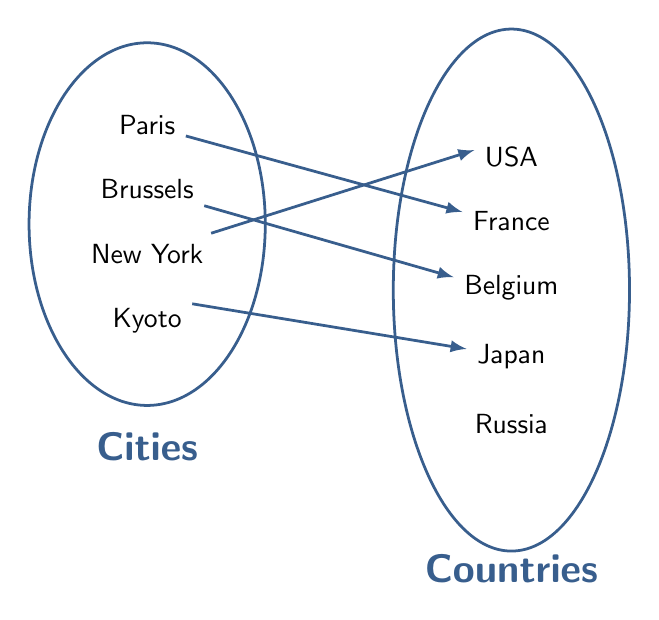
\begin{tikzpicture}[line width=1pt,>=latex]
\sffamily
\node (a1) {Paris};
\node[below=0.3cm of a1] (a2) {Brussels};
\node[below=0.3cm of a2] (a3) {New York};
\node[below=0.3cm of a3] (a4) {Kyoto};

\node[right=4cm of a1] (aux1) {};
\node[below= 0.0055cm of aux1] (b1) {USA};
\node[below=0.3cm of b1] (b2) {France};
\node[below=0.3cm of b2] (b3) {Belgium};
\node[below=0.3cm of b3] (b4) {Japan};
\node[below=0.3cm of b4] (b5) {Russia};
\node[below=0.005cm of b5] (aux2) {};

\node[shape=ellipse,draw=myblue,minimum size=3cm,fit={(a1) (a4)}] {};
\node[shape=ellipse,draw=myblue,minimum size=3cm,fit={(aux1) (aux2)}] {};

\node[below=1cm of a4,font=\color{myblue}\Large\bfseries] {Cities};
\node[below=1cm of aux2,font=\color{myblue}\Large\bfseries] {Countries};

\draw[->,myblue] (a1) -- (b2.170);
\draw[->,myblue] (a2) -- (b3.170);
\draw[->,myblue] (a3) -- (b1.170);
\draw[->,myblue] (a4.20) -- (b4.170);
\end{tikzpicture}
\end{center}
 
\noindent The set on the left has 4 elements, all are cities in the world, and the one on the right has 5 elements all of them countries. I drew a \textbf{relation} between the two sets, represented by all the arrows\footnote{The set of departure is called the \textbf{domain}, in this case the set of the cities. The destination set is called the \textbf{codomain}}. The relation depicted is "\textit{is a city in}". But I could have chosen a different relation, for instance "is on the same continent as", which looks like below:
\begin{center}
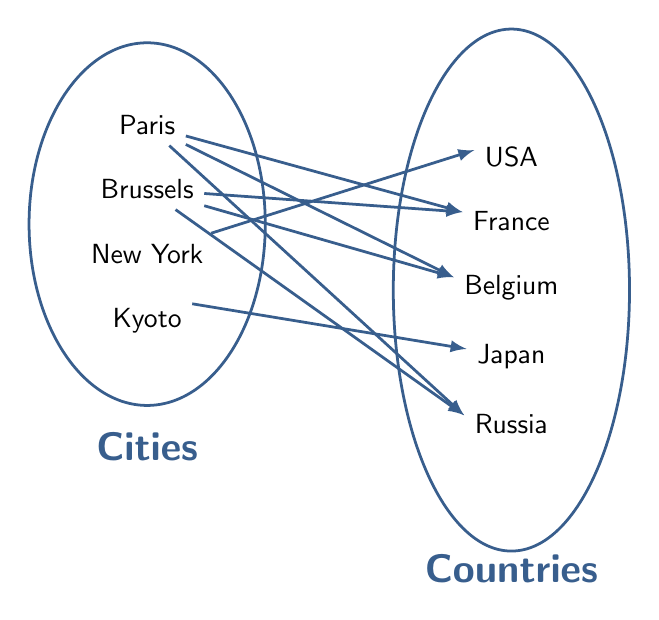
\begin{tikzpicture}[line width=1pt,>=latex]
\sffamily
\node (a1) {Paris};
\node[below= 0.3cm of a1] (a2) {Brussels};
\node[below=0.3cm of a2] (a3) {New York};
\node[below=0.3cm of a3] (a4) {Kyoto};

\node[right=4cm of a1] (aux1) {};
\node[below= 0.0055cm of aux1] (b1) {USA};
\node[below=0.3cm of b1] (b2) {France};
\node[below=0.3cm of b2] (b3) {Belgium};
\node[below=0.3cm of b3] (b4) {Japan};
\node[below=0.3cm of b4] (b5) {Russia};
\node[below=0.005cm of b5] (aux2) {};

\node[shape=ellipse,draw=myblue,minimum size=3cm,fit={(a1) (a4)}] {};
\node[shape=ellipse,draw=myblue,minimum size=3cm,fit={(aux1) (aux2)}] {};

\node[below=1cm of a4,font=\color{myblue}\Large\bfseries] {Cities};
\node[below=1cm of aux2,font=\color{myblue}\Large\bfseries] {Countries};

\draw[->,myblue] (a1) -- (b2.170);
\draw[->,myblue] (a1) -- (b3.170);
\draw[->,myblue] (a1) -- (b5.170);
\draw[->,myblue] (a2) -- (b2.170);
\draw[->,myblue] (a2) -- (b3.170);
\draw[->,myblue] (a2) -- (b5.170);
\draw[->,myblue] (a3) -- (b1.170);
\draw[->,myblue] (a4.20) -- (b4.170);
\end{tikzpicture}
\end{center}
\noindent Now that I've introduced the notion of "relation between sets", we can approach the question of equal sizes. The sets of cities and of countries above clearly do not have an equal number of elements. We can simply count them: $4$ in the domain and $5$ in the codomain.\\

\noindent Let us now consider a more abstract example:
\begin{center}
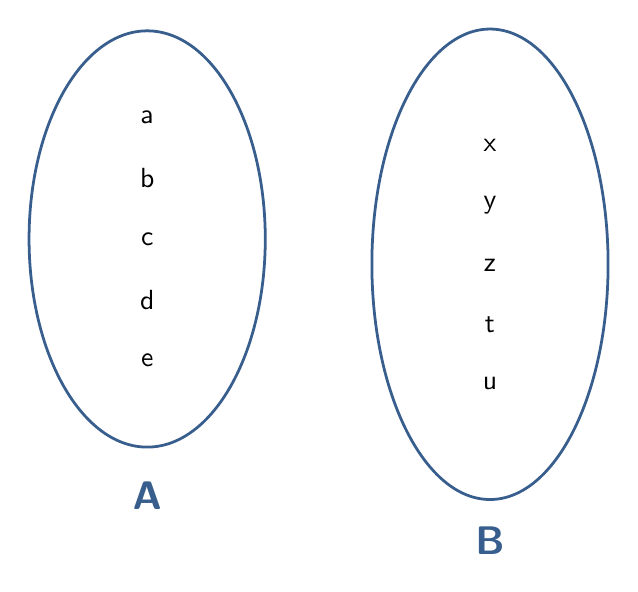
\begin{tikzpicture}[line width=1pt,>=latex]
\sffamily
\node (a1) {a};
\node[below=0.3cm of a1] (a2) {b};
\node[below=0.3cm of a2] (a3) {c};
\node[below=0.3cm of a3] (a4) {d};
\node[below=0.3cm of a4] (a5) {e};

\node[right=4cm of a1] (aux1) {};
\node[below= 0.0055cm of aux1] (b1) {x};
\node[below=0.3cm of b1] (b2) {y};
\node[below=0.3cm of b2] (b3) {z};
\node[below=0.3cm of b3] (b4) {t};
\node[below=0.3cm of b4] (b5) {u};
\node[below=0.005cm of b5] (aux2) {};

\node[shape=ellipse,draw=myblue,minimum size=3cm,fit={(a1) (a5)}] {};
\node[shape=ellipse,draw=myblue,minimum size=3cm,fit={(aux1) (aux2)}] {};

\node[below=1.2cm of a5,font=\color{myblue}\Large\bfseries] {A};
\node[below=1.2cm of aux2,font=\color{myblue}\Large\bfseries] {B};
\end{tikzpicture}
\end{center}
\noindent We have here a domain and codomain, each with $5$ elements. Let us consider two relations between those sets. The first one is:\\
\begin{center}
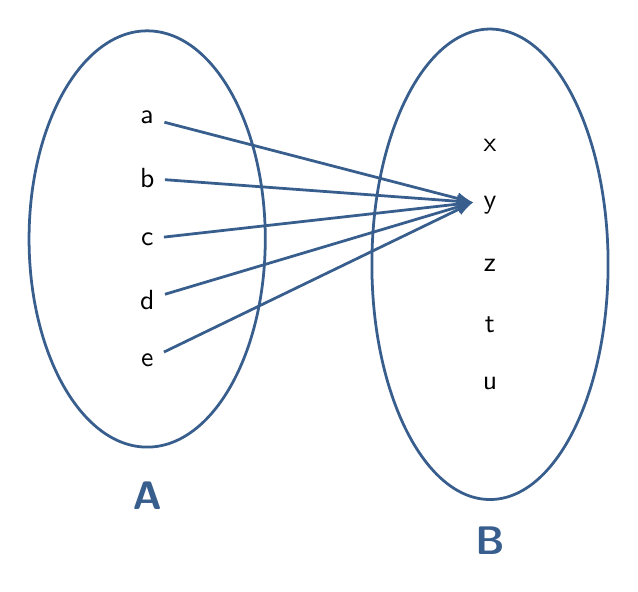
\begin{tikzpicture}[line width=1pt,>=latex]
\sffamily
\node (a1) {a};
\node[below=0.3cm of a1] (a2) {b};
\node[below=0.3cm of a2] (a3) {c};
\node[below=0.3cm of a3] (a4) {d};
\node[below=0.3cm of a4] (a5) {e};

\node[right=4cm of a1] (aux1) {};
\node[below= 0.0055cm of aux1] (b1) {x};
\node[below=0.3cm of b1] (b2) {y};
\node[below=0.3cm of b2] (b3) {z};
\node[below=0.3cm of b3] (b4) {t};
\node[below=0.3cm of b4] (b5) {u};
\node[below=0.005cm of b5] (aux2) {};

\node[shape=ellipse,draw=myblue,minimum size=3cm,fit={(a1) (a5)}] {};
\node[shape=ellipse,draw=myblue,minimum size=3cm,fit={(aux1) (aux2)}] {};

\node[below=1.2cm of a5,font=\color{myblue}\Large\bfseries] {A};
\node[below=1.2cm of aux2,font=\color{myblue}\Large\bfseries] {B};

\draw[->,myblue] (a1) -- (b2.170);
\draw[->,myblue] (a2) -- (b2.170);
\draw[->,myblue] (a3) -- (b2.170);
\draw[->,myblue] (a4) -- (b2.170);
\draw[->,myblue] (a5) -- (b2.170);
\end{tikzpicture}
\end{center}

\noindent From each element in $A$ there is exactly 1 arrow leaving. In $B$ all arrows arrive in $y$. None of the other elements in $B$ has an arrow arriving at it.\\

\noindent The second relation we consider between $A$ and $B$ is:\\
\begin{center}
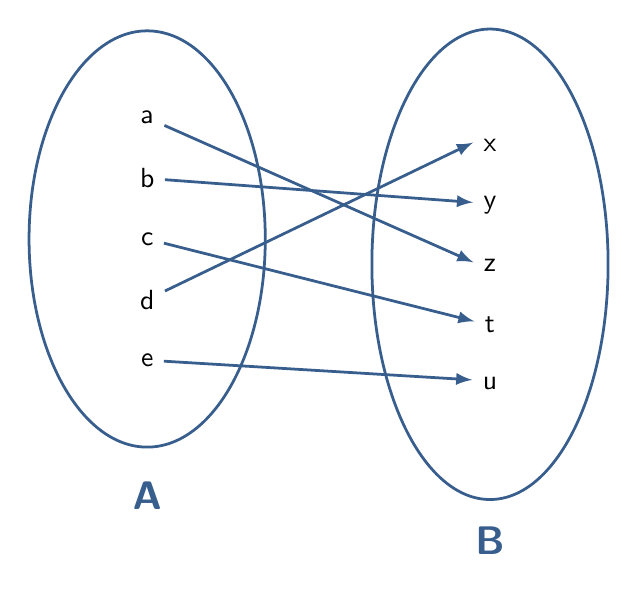
\begin{tikzpicture}[line width=1pt,>=latex]
\sffamily
\node (a1) {a};
\node[below=0.3cm of a1] (a2) {b};
\node[below=0.3cm of a2] (a3) {c};
\node[below=0.3cm of a3] (a4) {d};
\node[below=0.3cm of a4] (a5) {e};

\node[right=4cm of a1] (aux1) {};
\node[below= 0.0055cm of aux1] (b1) {x};
\node[below=0.3cm of b1] (b2) {y};
\node[below=0.3cm of b2] (b3) {z};
\node[below=0.3cm of b3] (b4) {t};
\node[below=0.3cm of b4] (b5) {u};
\node[below=0.005cm of b5] (aux2) {};

\node[shape=ellipse,draw=myblue,minimum size=3cm,fit={(a1) (a5)}] {};
\node[shape=ellipse,draw=myblue,minimum size=3cm,fit={(aux1) (aux2)}] {};

\node[below=1.2cm of a5,font=\color{myblue}\Large\bfseries] {A};
\node[below=1.2cm of aux2,font=\color{myblue}\Large\bfseries] {B};

\draw[->,myblue] (a1) -- (b3.170);
\draw[->,myblue] (a2) -- (b2.170);
\draw[->,myblue] (a3) -- (b4.170);
\draw[->,myblue] (a4) -- (b1.170);
\draw[->,myblue] (a5) -- (b5.170);
\end{tikzpicture}
\end{center}

\noindent This relation has the special property that exactly 1 arrow leaves each element in the domain and exactly 1 arrow arrives at each element of the codomain. A relation with this property is called a \textbf{bijection}.\\

\noindent If 2 sets have an equal number of elements, it is possible to find a bijection between them. On the other hand, if they do not contain an equal number of elements it is impossible to find a bijection between them. It seems reasonable that if the number of elements in the sets is different, it will be impossible to find a relation where exactly 1 arrow leaves every element in the domain and exactly 1 arrow arrives at each element in the codomain.\\

\noindent \textbf{Mistake to avoid:} The claim is that a bijection can be found if both sets have an equal number of elements. However, this does \textbf{not} imply that every relation between both sets is a bijection. The first relation we considered above between $A$ and $B$ is clearly not a bijection despite $A$ and $B$ each containing $5$ elements.

\subsection{Counting the infinite}
\label{Cantor_Tangent}

\noindent For infinite sets we use the same logic. We say that if it is possible to find a bijection between 2 infinite sets, they contain the same number of elements\footnote{The number of elements is of course infinite, and not actually a number. Mathematicians therefore invented the word "`cardinality"'. For finite sets the cardinality of a set is equal to its number of elements. Infinite sets are said to have the same cardinality if they "`contain the same number of elements"'}. The question whether $\mathbb{N}$ and $\mathbb{Z}$ have the same number of elements is reduced to determining whether a bijection between them exists.\\

\noindent One possible relation between them is the following:
\begin{eqnarray*}
0 & \rightarrow & 0  \\
1 & \rightarrow & 1  \\
2 & \rightarrow & -1 \\
3 & \rightarrow & 2  \\
4 & \rightarrow & -2  \\
5 & \rightarrow & 3  \\
 & \cdots & 
\end{eqnarray*}
On the left are the elements of $\mathbb{N}$ and on the right those of $\mathbb{Z}$. There is exactly 1 arrow leaving each element of $\mathbb{N}$ and exactly 1 arrow arriving at each element of $\mathbb{Z}$. This relation is therefore a bijection, which proves that the two sets have the "`same number of elements"'.\\

\noindent You could very well think that it is possible to find a bijection between any 2 infinite sets, after all they're both infinite. In that case you would be wrong.\\

\noindent It turns out that it is impossible to find a bijection between $\mathbb{N}$ and $\mathbb{R}$. But how could we prove that a bijection between them does not exist? There are infinitely many relations we could write down. How can we go through all of them and be sure we didn't miss any, before concluding that there does not exist any bijection between them?\\

\noindent We will divide the argument into 2 parts. The first one will be to prove there cannot exist a bijection between $\mathbb{N}$ and $\left[ 0 , 1 \right[$ which is the set of all real numbers between $0$ and $1$ (including $0$ but excluding $1$)\footnote{The set $\left[ 0,1 \right[$ includes $0$ but not $1$, while $\left] 0,1 \right]$ includes $1$ but not $0$. Finally, $\left] 0,1 \right[$ excludes them both.}. From this we conclude that these 2 sets do not have the same "`number of elements"'. The second part of the proof will be to show that there exists a bijection between $\mathbb{R}$ and $\left[  0,1 \right[$. From which we conclude that these two sets do have the same number of elements. Taking these two parts together does indeed prove that $\mathbb{N}$ and $\mathbb{R}$ do not have the same "`number of elements"'.\\

\noindent We start part 1 of the argument by assuming there does exist a bijection between $\mathbb{N}$ and $\left[ 0,1 \right[$. We will see that this assumption will lead to an impossible result, which means that the assumption itself cannot be true.\\

\noindent So let us assume such a bijection exists. It can be represented as:
\begin{eqnarray*}
0 & \rightarrow & x_0  \\
1 & \rightarrow & x_1  \\
2 & \rightarrow & x_2 \\
3 & \rightarrow & x_3  \\
4 & \rightarrow & x_4  \\
5 & \rightarrow & x_5  \\
 & \cdots & 
\end{eqnarray*}
The numbers $x_0, x_1,\cdots$ are all real numbers between $0$ and $1$ (excluding $1$ itself), all different from each other (otherwise there would be 2 arrows arriving at the same element of $[0,1[$ and it wouldn't be a bijection) and each of them can be written in decimal form. As we assumed the relation is a bijection, exactly 1 arrow arrives at each element of $\left[ 0,1 \right[$, and it should therefore not be possible to find any number between 0 and 1 that does not appear in our list of $x_i$'s.\\

\noindent I will now find a number that does not appear in the list by the following method:
\begin{enumerate}
\item Call the number between 0 and 1 that we are looking for $x$. We know $x$ starts of with a $0$ before the decimal point (because it's between 0 and 1). 
\item If the first decimal of $x_0$ is not a 5, we choose the first decimal of $x$ equal to 5. Otherwise we choose the first decimal of $x$ equal to 4.
\item  If the second decimal of $x_1$ is not a 5, we choose the second decimal of $x$ equal to 5. Otherwise we choose the second decimal of $x$ equal to 4.
\item If the third decimal of $x_2$ is not a 5, we choose the third decimal of $x$ equal to 5. Otherwise we choose the third decimal of $x$ equal to 4.\\
$\cdots$
\end{enumerate}
\noindent This procedure is known as Cantor's diagonalization. The number $x$ we end up with is clearly a number between 0 and 1. It differs from $x_0$ because their first decimal is unequal. It differs from $x_1$ because their second decimal is unequal. It differs from $x_{37}$ because their thirty-eighth decimal is unequal, etc. It thus differs from each of the $x_i$'s. That means that we found an element of $\left[ 0 , 1 \right[$ which differs from all of the $x_i$'s and therefore does not appear in the list. In other words it does not have an arrow arriving at it. Which means the relation we assumed to be a bijection is not a bijection. A relation cannot be a bijection and not a bijection at the same time. We conclude that our initial assumption is wrong. As our argument holds for any relation between $\mathbb{N}$ and $\left[ 0,1 \right[$ there can not exist a bijection between them.\\

\noindent This concludes part 1 of the proof. We still need to do part 2, which is to prove that $\mathbb{R}$ and $\left[ 0,1 \right[$ do have the same size. I will leave this final step for after we handle trigonometric functions in section (\ref{TrigFuncs}) because one of them (the tangent) will be a natural candidate for the bijection between the two sets.

% Maybe add at later time also proof that pi is irrational
\chapter{Basic operations}

\section{Addition, subtraction, multiplication and division}

\noindent Here we present the most basic mathematical operations on the real numbers. We will only mention shortly the main properties as a reminder.

\subsection{Basic operations on real numbers}

\subsubsection{Addition}

\noindent Take any two real numbers $a$ and $b$. It is true no matter what $a$ and $b$ are that
$$
a + b = b + a
$$
Mathematicians call this property commutativity and say that the sum of two real numbers is commutative. But that is just a fancy word. And we should not focus on names. Basically, the order of adding two numbers does not affect the result.

\subsubsection{Subtraction}

\noindent We remain with our numbers $a$ and $b$. By $-b$ we mean the number you get when changing $b$'s sign. Notice that $-b$ isn't necessarily negative. If $b$ itself is negative, changing its sign will make it positive and so $-b$ will be positive in such a case.\\

\noindent The difference of $a$ and $b$ is then defined as
$$
a - b = a + (-b)
$$
In words, take the numbers $a$ and $b$, change the sign of $b$ and add $-b$ to $a$.\\

\noindent Because the sum is commutative it follows that
$$
a - b = a + (-b) = -b + a
$$
But unlike addition, the order of the numbers in a subtraction cannot be reversed without changing the result:
$$
a - b \neq b - a
$$
Changing the order of the subtraction amounts to changing the sign of the result:
$$
a - b = -(b-a)
$$

\subsubsection{Multiplication}

\noindent Writing a sum can be tedious:
\begin{equation*}
5 + 5 + 5 + 5 + 5 + 5 + 5 = 35
\end{equation*}
A multiplication is in the simplest case a shorthand notation for this. The number 5 is added 7 times here, which is written as: $ 5 \times 7 $.\\

\noindent As was the case for the addition, the multiplication is commutative:
\begin{equation*}
4 \times 8 = 8 \times 4
\end{equation*}
This equality says that $8+8+8+8 = 4+4+4+4+4+4+4+4$, which is true.\\

\noindent Multiplying 2 positive numbers or 2 negative numbers yields a positive result. When one of the numbers is positive and the other is negative the result is negative. And multiplying any number by 0 always gives 0.
\begin{eqnarray*}
-5 \times 9 & = & -45 \\
17 \times 0 & = & 0 \\
-6 \times (-8) & = & 48
\end{eqnarray*}
\noindent As we will soon get to equations and variables in our discussion of mathematics, it may get confusing if we use the symbol $\times$ for multiplication and $x$ for a variable. In order to avoid confusion we will often write multiplications with a "." symbol: $3 \times 4 = 3 . 4$. The symbols "$.$" and "$\times$" both represent the same action of multiplying the numbers on either side of them with each other, and they will be used interchangeably throughout the rest of the text. Additionally, when representing numbers by letters, we will often omit any sign of multiplication all together: $a \times b = a . b = ab$. They all mean $a$ times $b$. We have actually already done this earlier in the text when we discussed properties of rational numbers in chapter \ref{Set_Theory}. We wrote there $1\: 000 \: x$ which means one thousand times $x$, though we omitted and sign of multiplication.

\subsubsection{Division}

\noindent The division is the inverse function of the multiplication. This means that if $a \times b = c$ then $a = \frac{c}{b}$ or equally $b = \frac{c}{a}$.
$$
\frac{63}{7} = 9 \text{ is equivalent with } 7 \times 9 = 63
$$
\noindent Division of $a$ and $b$ is written as $\frac{a}{b}$ or as $a \div b$.\\

\noindent \textbf{Point of attention:} The denominator in a division is never allowed to be zero. We will see when discussing the concept of limits how cases that look like a division by zero can be handled. But as such, dividing by zero is a very big no-no in mathematics.

\subsection{Basic operations of fractions}

\noindent A fraction is nothing more than a division that still needs to be done. It is of the form $\frac{a}{b}$ where $a$ is called the numerator and $b$ the denominator. The denominator has to be different from 0.

\subsubsection{Simplifying fractions}

\noindent Two fractions are equal when the result of the division of numerator by denominator is equal:
\begin{equation*}
\frac{1}{2} = 0.5 = \frac{8}{16}
\end{equation*}
A fraction remains unchanged when multiplying or dividing both numerator and denominator by the same number as this operation does not change the final result of their division:
\begin{equation*}
\frac{4}{15} = \frac{4 \times 3}{15 \times 3} = \frac{12}{45}
\end{equation*}
As you can easily check these 2 fractions indeed yield the same result when dividing numerator by denominator. Simplifying a fractions means getting rid of all the common factors in numerator and denominator. The fraction $\frac{144}{20}$ can be simplified to $\frac{36}{5}$. To do this we write it as
\begin{eqnarray*}
\frac{144}{20} = \frac{4 \times 36}{4 \times 5}
\end{eqnarray*}
\noindent By canceling out the $4$, which is a common factor in the numerator and denominator, we are indeed left with $\frac{36}{5}$ which does not have any remaining common factors.\\

\subsubsection{Addition and subtraction of fractions}

\noindent When adding (subtracting) fractions we need to make sure they have the same denominator. When the denominators are the same, the sum (difference) of the fractions is the sum (difference) of the numerators divided by their common denominator:
\begin{eqnarray*}
\frac{5}{2} + \frac{17}{2} = \frac{22}{2} = \frac{11}{1} = 11\\
-\frac{33}{16} + \frac{1}{16} = -\frac{32}{16} = -\frac{2}{1} = -2
\end{eqnarray*} 
When the denominators are unequal, we need to multiply both numerator and denominator by some number so as to make both the denominators equal:
\begin{equation*}
\frac{8}{3} - \frac{17}{12} = \frac{4 \times 8}{4 \times 3} - \frac{17}{12} = \frac{32}{12} - \frac{17}{12} = \frac{15}{12} = \frac{5}{4}
\end{equation*}
In this example it was sufficient to multiply the numerator and denominator of only one of the fractions by a number. In some other case it may be necessary to multiply both fractions:
\begin{equation*}
\frac{8}{3} - \frac{17}{4} = \frac{4 \times 8}{4 \times 3} - \frac{3 \times 17}{3 \times 4} = \frac{32}{12} - \frac{51}{12} = -\frac{19}{12}
\end{equation*}

\noindent \textbf{Point of notation:} The sum (difference) of fractions with the same denominator is often written as
$$
\frac{a}{c} \pm \frac{b}{c} = \frac{a \pm b}{c} 
$$

\subsubsection{Multiplication and division of fractions}

\noindent The multiplication of fractions comes down to multiplying the numerators and multiplying the denominators separately:
\begin{equation*}
\frac{a}{b} \times \frac{c}{d} = \frac{a \times c}{b \times d}
\end{equation*}
An example:
\begin{equation*}
\frac{4}{5} \times \frac{9}{2} = \frac{36}{10}
\end{equation*}
This fraction can still be simplified by dividing both numerator and denominator by $2$:
$$
\frac{36}{10} = \frac{18}{5}
$$
Dividing by a fraction is done by multiplying the first fraction by the inverse of the second fraction:
$$
\frac{a}{b} \div \frac{c}{d} = \frac{a}{b} \times \frac{d}{c} = \frac{a \times d}{b \times c}
$$
So that
\begin{equation*}
\frac{4}{5} \div \frac{9}{2} = \frac{4}{5} \times \frac{2}{9} = \frac{8}{45}
\end{equation*}
Dividing two numbers $a$ and $b$ is identical to multiplying $a$ with the inverse of $b$:
$$
\frac{a}{b} = a \times \frac{1}{b}
$$
This is consistent with the way multiplication of fractions was defined:
\begin{equation*}
5 \times \frac{1}{23} = \frac{5}{1} \times \frac{1}{23} = \frac{5 \times 1}{1 \times 23} = \frac{5}{23}
\end{equation*}
That is all there is to fractions...

\subsection{$\Sigma$: a shorthand notation for a sum}

\noindent The Greek capital letter $\Sigma$ (sigma) is used to shorten the writing of sums. Writing the sum of the 8 first (strictly) positive integers looks like
$$
1 + 2 + 3+ 4 + 5 + 6 + 7 + 8  = 36
$$
You will probably agree that this is a non-attractive, long-looking expression. The way a mathematician would write this is
$$
\sum\limits_{i = 1}^{8} i = 36
$$
This should be read as "the sum of $i$, for $i$ going from 1 to 8". In this expression the index $i$ is called a dummy index. It has no meaning as such. The information under the $\Sigma$ tells us that the first value that is plugged in to $i$, which in this example is 1. Then we write a plus and plug in the next value of $i$ which is 2. Then we write a plus...\\
And this is done until the last value of $i$ which is the value at the top of the $\Sigma$, in this case it's 8.\\

\noindent A couple of examples:
\begin{eqnarray*}
\sum\limits_{i = 0}^{5} \left( i\times i \right) &  = & 0\times 0 + 1 \times 1 + 2\times 2 + 3 \times 3 + 4 \times 4 + 5\times 5 = 55 \\
\sum\limits_{i = 3}^{6} \left(2i + 1\right) & = & 7 + 9 + 11 + 13 = 40 \\
\sum\limits_{i = 1}^{10} 3 & = & \underbrace{3 + 3 + 3 +\cdots + 3}_{10 \; terms} = 30\\ 
\sum\limits_{k = 2}^{6} \left( -\frac{2}{k}\right) &= & -\frac{2}{2} -\frac{2}{3} -\frac{2}{4}-\frac{2}{5} -\frac{2}{6} = -\frac{60 + 40 + 30 + 24 + 20}{60} = -\frac{174}{60} =  - \frac{29}{10}
\end{eqnarray*}
Notice in the third example the lack of "`$i$"' in the expression on the left hand side (LHS). The value to be summed remains 3 regardless of the value of $i$. Therefore we have to add a 3 for each value that $i$ can take, which is 10 in this case. In the last example we changed the letter we use as a dummy index from $i$ to $k$. This is always allowed as the dummy index has no meaning of its own. It is just a placeholder for whatever number we are going to plug in the expression.

\section{exponents, roots and absolute value}

\subsubsection{Positive integer exponents}

\noindent In the same way that a multiplication is a shorthand notation for a sum, an exponential is a shorthand notation for a multiplication:
\begin{eqnarray*}
6 \times 6 \times 6 & =  6^3 & =  216 \\
4 \times 4 \times 4 \times 4 & =  4^4 & =  256
\end{eqnarray*}
More generally, for any real number $a$ and any (strictly) positive integer $b$:
$$
a^b = \underbrace{a \times a \times \cdots \times a}_{b \; factors}
$$
where $a$ is called the base number and $b$ the exponent. We say "`$a$ to the power $b$"' or simply "`$a$ to the $b$-th"'.\\

\noindent From the definition it follows that $1^b$ = 1, no matter what the value of b is. If the exponent is 0 the result is by definition 1: $a^0 = 1$. The only exception to this is if $a$ itself is equal to 0 too, in which case it is simply not defined. So $0^0$ should never be used cause it is simply "bla".\\

\noindent If $b$ and $c$ are 2 positive integers than
$$
a^b \times a^c = \underbrace{a \times a \times \cdots \times a}_{b \; factors} \times \underbrace{a \times a \times \cdots \times a}_{c \; factors} = \underbrace{a \times a \times \cdots \times a}_{b+c \; factors} = a^{b+c}
$$
Another property which follows from the definition is
$$
\left( a^b \right)^c = \underbrace{a^b \times a^b \times \cdots \times a^b}_{c \; factors} = \overbrace{a^{b + b + \cdots + b}}^{c \; terms} = a^{b \times c} 
$$

\subsubsection{Negative integer exponents}

\noindent The negative (integer) exponent is defined as:
$$
a^{-b} = \frac{1}{a^b}
$$
So that
\begin{eqnarray*}
2^{-3} = \frac{1}{2^3} = \frac{1}{8} = 0,125 \\
\left( \frac{3}{5} \right)^{-4} = \frac{1}{\left( \frac{3}{5} \right)^4} = \left( \frac{5}{3} \right)^4 = \frac{5^4}{3^4} = \frac{625}{81}
\end{eqnarray*}

\subsubsection{Square root}

\noindent The square root is the inverse function of taking the square. This means
$$
a^2 = b \Leftrightarrow \sqrt{b} = a
$$
Examples are
\begin{eqnarray*}
\sqrt{16} = \pm 4 & \text{because} & \left( \pm 4 \right)^2 = 16 \\
 \sqrt{121} = \pm 11 & \text{because} & \left( \pm 11 \right)^2 = 121
\end{eqnarray*}
Notice that a square root has 2 results, because multiplying two positive reals as well as 2 negative reals gives a positive result. It is impossible to find a real number whose square is negative. Therefore the square root of a negative number doesn't exist\footnote{We will see later that there are indeed number whose square is negative, but these numbers do not belong to $\mathbb{R}$ and we can forget about them for the time being}.

\subsubsection{Other roots}

\noindent We saw that the square root is the inverse function of the square, i.e. taking the second power. More generally, the inverse function of taking any power is called a root. It is denoted as
$$
a^n = b \Leftrightarrow \sqrt[n]{b} = a
$$
In words: "`if the n-th power of a is b if and only if the \textbf{n-th root} of b is a"'. For example:
\begin{eqnarray*}
\sqrt[3]{8} =  2 & \text{because} & \left(  2 \right)^3 = 8 \\
 \sqrt[4]{81} = \pm 3 & \text{because} & \left( \pm 3 \right)^4 = 81
\end{eqnarray*}
Note that for even powers there are 2 results possible, because taking an even power of a base number or of the negative of the base number gives the same result.\\

\noindent The exponent we considered in the previous sections were integers. We now define the meaning of rational exponents. We take numbers $a,b$ and $c$ with the conditions that $c \neq 0 $, $b \in \mathbb{Z}$ and $a^b$ is non-negative if $c$ is even:  
$$
a^{\frac{b}{c}} =  \sqrt[c]{a^b}
$$
So that
\begin{eqnarray*}
4^{2,5}=4^{\frac{5}{2}} = \sqrt{4^5} = \sqrt{1024} = 32 \\
\left( -1,3 \right)^{-3,8} = \left( - \frac{13}{10} \right)^{-\frac{19}{5}} = \left( - \frac{10}{13} \right)^{\frac{19}{5}} = \left( \sqrt[5]{-\frac{10}{13}} \right)^{19} = -2,71
\end{eqnarray*}
The last example thus means that $\left( -2,71 \right)^{-\frac{1}{3,8}}$ = -1,3

\subsubsection{Absolute value}

\noindent The absolute value of a real number a is defined as:
$$
|a| = \left\{ \begin{array}{ll}
                  a \ \ \ \ \ \  \text{if } a \geq 0 \\
                  -a \ \ \ \ \ \  \text{if } a < 0 
                \end{array}
              \right.
$$
So if $a$ is positive or zero, then $|a| = a$, and if $a$ is negative then $|a| = -a$. Basically the absolute value is simply the real number where the minus sign, if there is one, is omitted:
\begin{eqnarray*}
 |19| = 19 \\
|-3| = 3 \\
|0| = 0
\end{eqnarray*}

\section{Order of operations}

\noindent How should an expression like the below be interpreted?
$$
2 + 3 \times 4
$$
\noindent If we were to read it from left to right the result would be $20$. We would start by adding $2$ and $3$ to get $5$. And multiply this $5$ by $4$ to get $20$. But this is wrong.\\

\noindent The convention in mathematics is to give precedence to multiplication and division, and only then do subtraction and addition. In the calculation above we thus first multiply $3$ by $4$ which is $12$. And then add $2$ to find the correct result of $14$.\\

\noindent Generally the convention is that operations have to be executed in the following order:
\begin{enumerate}
\item brackets
\item exponents 
\item multiplication and division
\item addition and subtraction
\end{enumerate}
\noindent Remember that roots, square or otherwise, are exponents and should therefore be treated as such.
\noindent Here are a couple of examples:
\begin{itemize}
\item $1 + 4 : 2 + 3 = 1 + 2 + 3 = 6$ 
\item $(1+4) : (2 + 3) = 5 : 5 = 1 $
\item $(1+4):2 + 3 = 5:2 + 3 = 2.5 + 3 = 5.5$
\item $\sqrt{5+4} : 2-3 = \sqrt{9} : 2 - 3 = 3 : 2 - 3 =  1.5 - 3 = -1.5$
\item $(3 + 8) \times (7-4) =  11 \times 3 = 33$
\item $(2+4)^3 = 6^3 = 216$
\item $(3 \times (12:4)^3 - 14) \times 2 = (3 \times 3^3 - 14) \times 2 = (81 - 14) \times 2 = 67 \times 2 = 134$
\item $\frac{1+2}{3+4} + 5 = \frac{3}{7} + 5 = 0.42857 + 5 = 5.42857$
\end{itemize}
\noindent In the last example we first worked out the sums in the fraction. Writing a fraction as in the last example should be interpreted as having brackets in the numerator and denominator:
$$
\frac{1+2}{3+4} + 5 = \frac{(1+2)}{(3+4)} + 5
$$

\section{Go and multiply!}

\noindent Keeping in mind the order of the operations, we do the following calculation:
\begin{eqnarray*}
(3+4)^2 & = & (3+4) \times (3+4) \\
& = & 7 \times 7 \\
& = & 49
\end{eqnarray*}
\noindent We get the same result if the brackets are worked out term by term:
\begin{equation*}
     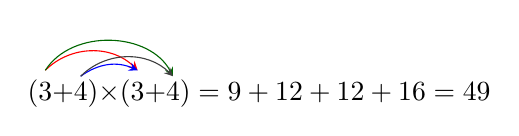
\begin{tikzpicture}[>=stealth,baseline,anchor=base,inner sep=0pt]
       \matrix (foil) [matrix of math nodes,nodes={minimum height=0.5em}] {
         ( & 3 & + & 4 & ) & \times & ( & 3 & + & 4 & ) = 9 + 12 + 12 + 16 = 49\\
       };
       \path[->] ($(foil-1-2.north)+(0,1ex)$)   edge[red,bend left=45]    ($(foil-1-8.north)+(0,1ex)$)
                 ($(foil-1-2.north)+(0,1ex)$)   edge[green!40!black,bend left=60]  ($(foil-1-10.north)+(0,0.5ex)$)
                 ($(foil-1-4.north)+(0,0.5ex)$) edge[blue,bend left]      ($(foil-1-8.north)+(0,1ex)$)
                 ($(foil-1-4.north)+(0,0.5ex)$) edge[darkgray,bend left=45] ($(foil-1-10.north)+(0,0.5ex)$);
     \end{tikzpicture}
   \end{equation*}
\noindent This property is known as \textbf{distributivity of multiplication over addition} and holds generally:
\begin{equation*}
(a+b)^2=(a+b)  (a+b) = a^2 + a b + b  a + b^2 = a^2 + 2 a  b + b^2
\end{equation*}
Where we used the commutativity of the multiplication of numbers: $a\times b = b \times a$.\\

\noindent Use distributivity to convince yourself of the following identities:
\begin{center}
\begin{tabular}{ |c| }
  \hline
  $(a+b)^2 =  a^2 + 2ab + b^2$\\
  $(a-b)^2 =  a^2 - 2ab + b^2$\\
	$(a+b)(a-b) =   a^2 - b^2$\\
	$(a+b)^3 =  a^3 + 3 a^2b + 3 ab^2 + b^3$\\
	\hline
\end{tabular}
\end{center}
\chapter{The patterns we experience, the laws we accept}
\label{Intro_Physics}

\epigraph{The good thing about science is that it's true whether or not you believe in it}{\textit{ Neil DeGrasse Tyson}}

\section{Science doesn't know everything!}

\noindent We observe patterns of reality. The sun rises every morning. So we postulate that it will rise tomorrow too. And the day after. And the day after that. This pattern does not seem to change. Though the details of exactly at what time this happens, how long it takes for the sun to rise from over the horizon to its zenith, the angle under which it does so, the heat it radiates... do vary when looked at closely. But despite these differences there is a clear pattern to discern. We are convinced the sun will rise tomorrow. It is not impossible we are wrong about this. But all the evidence at hand does not contradict this prediction, it corroborates it.\\

\noindent Science does not know everything. Far from it. But to quote the comedian/physicist Dara O'Briain: "Science knows it doesn't know everything. Otherwise, it'd stop!".\\

\noindent Many claims have been made and tested. Some turned out to be in contradiction with what actually happens in reality. We know that these claims that have been falsified are untrue. There is therefore quite a bit that science does know, insofar as one can know anything.\\ 

\noindent In this chapter I have two main goals:
\begin{enumerate}
\item Discuss a number of these topics about which we do know quite a lot. 
\item Introduce a number of ideas and topics in physics without diving into the hard quantitative descriptions just yet. I will mostly omit math in this chapter and will focus on the concepts. In later chapter we will revisit many of these topics and include the mathematical description of them.
\end{enumerate}

\section{Newton's laws}

\noindent Mechanics, the body of knowledge concerning motion: how do objects move and why do they move that way. Traditionally one of the first topics treated in physics. And the basics of mechanics are given by Newton's three laws of motion.

\begin{enumerate}

\item \textbf{Newton's first law:} Any object remains in its state of motion, unless it is acted upon by a force.\\

\noindent Objects that are moving will keep on moving with the same speed in the same direction forever, unless a force compels them otherwise. Objects that are standing still will remain still unless a force compels them otherwise. This phenomenon is called \textbf{inertia}. This is the first of several instances in which we use a word used in daily life but meaning something (slightly) different in physics. Be aware of these differences as they may be the source of confusion or misunderstanding.\\

\noindent We experience inertia in several everyday circumstances:
\begin{itemize}
\item Sitting in a car that suddenly brakes, we are thrown forwards. Without the seat belts we could be thrown straight out through the front shield. The car's breaks do stop the car but our body does not experience this and inertia keeps it moving forward.

\item Taking a turn with the car, we experience a force pushing us away from the direction towards which the car is turning. Inertia actually keeps us moving straight ahead, but as the car turns we experience this as if there were a force on us in the other direction. 

\item When standing on a bus we fall backwards when it starts moving. The engine forces the bus to move but our body remains where it was standing. We experience this as a force backward as seen from the bus.

\end{itemize}
 
\noindent So why does everything around seem to come to a standstill? Well, because the surface on which the object is moving, as well as the air around it exert a frictional force on the moving object which makes it stop. The first of Newton's law states that in the absence of such forces, once in motion the object remains indefinitely in motion. An astronaut drifting away from her space-shuttle will keep on drifting indefinitely.

\item \textbf{Newton's second law:} In the presence of forces the object's velocity changes. The mass of the object is a measure for the difficulty of changing its velocity.\\

\noindent The equation known as Newton's second law, describing the motion of an object is given in its simplest form by
\begin{equation}
F = m a
\end{equation}
where $F$ is the force exerted on the object, $m$ is its mass and $a$ its acceleration. The acceleration, as we will see in the near future, is nothing but the change of the velocity. Let us consider two objects at rest, one with mass = $2 kg$ and the other with mass $1\; 000 kg$. We exert an equal force on both objects, equal to 10 Newton\footnote{Just like the unit of mass is called kg, the unit of force is called Newton. We will see in the chapter on mechanics what a force of 1 Newton represents.}. Looking at their acceleration (i. e. we look at how fast they move after the force was applied) we notice the following:
\begin{center}
\begin{tabular}{|c|c|c|}
  \hline
	& & \\
  \textbf{Object} &2 kg  & 1\;000 kg \\
	\hline
  & & \\
	\textbf{Speed} & $5 m/s $ & $0,01 m/s $\\
  \hline
\end{tabular}
\end{center}
\noindent The lighter object's acceleration is greater than that of the heavier one under the influence of the same force.\\

\noindent Kicking a football lying on the ground will make it fly away. The same kick will not do anything noticeable to a train. Equal forces on vastly different masses have vastly different consequences.\\

\noindent The gravitational force that the earth exerts on a hanging apple is as strong as the gravitational force that the apple exerts on the earth. But it is clearly the apple falling towards the earth and not the other way around. Why? Because the earth is enormously heavier compared to apple. So the change of velocity of the apple is much larger than that of the earth.\\

\noindent Newton's second law contains much more information than I explain here. In the chapters on vectors and on mechanics we will deepen our understanding of the content of this law and its predicted physical consequences.\\

\item \textbf{Newton's third law:} Forces come in equal but opposite pairs.

\begin{itemize}
\item While ice-skating you push your friend away. Not only will you friend be pushed forward (i.e. away from you), but you yourself will be pushed backwards (i.e. away from your friend). You exert a force on her. And she consequently exerts a force on you of equal size and opposite direction to the original force.
\item A rocket forces fuel out of its tail. The fuel consequently exerts a equal force on the rocket upward, which causes it to accelerate upwards.
\end{itemize}

\end{enumerate}

\noindent When describing the motion of a football, a rocket, an elephant and more generally in "`everyday circumstances"' these three laws give an accurate representation of what actually happens. But only the first of the laws does not have any known exceptions. The second and third law are known not to correctly describe the very small, the very fast, the very heavy, the very warm, the very cold,...\\

\noindent In such cases other laws hold, some of which we will discuss further on in the text. So keep in mind that together with a physical theory come its limits of applicability. And using the theories outside these limits will result in false predictions about what reality will/may do under these circumstances.

\section{Unification: l'union fait la force!}

\noindent There are many known forces in physics: gravitational, van der Waals,  electrical, magnetic, nuclear, drag, lift, frictional, centripetal, centrifugal,...\\

\noindent However, it turns out that there are only four fundamental ones:
\begin{enumerate}
\item Gravity
\item Electromagnetism
\item Strong nuclear
\item Weak nuclear
\end{enumerate}
We will discuss each of them in due time. But for now, it is sufficient to know that we do not know any other forces. All the other forces like friction or the centripetal force are one or several of the fundamental forces in disguise. We will come back to this point later.\\

\noindent This section is about forces. But about their similarities rather than their differences.
\begin{itemize}
\item A magnet pushing another magnet away seems to be something very different from the spark you feel (and sometimes even see) when touching a car door on a dry day.
\item The needle of a compass reacting to the earth's magnetic field seems to be completely different from the lightning strike during a thunderstorm.
\item An apple falling seems to be unrelated to the way the our solar system moves within the milky way.
\end{itemize}
Remember that impressions can be misleading. In each of these examples the phenomena are not only related, but turn out to be a consequence of the same underlying mechanism. Realizing that seemingly different phenomena can be understood in the same way is known in physics as unification.\\

\noindent Isaac Newton himself realized that the fall of an apple and the motion of the heavenly bodies are both instances of gravitational forces. But it doesn't stop there. The tides of the sea, and the presence of an atmosphere on some planets and not on others as well as the chemical constitution of that atmosphere can be explained by the same phenomenon that makes an apple fall from the tree.

\noindent Michael Faraday, James Clerk Maxwell and other $19^{th}$ century scientists realized that electric and magnetic phenomena are very closely related. When electric phenomena are present, magnetic phenomena are rarely far away and vice versa. Albert Einstein understood a couple of decades later that electric and magnetic phenomena are in some sense the same phenomenon, that they are two sides of a same coin (see section \ref{ElectromagneticSection}). Sailing the seas in a thunderstorm you may notice that your compass loses all sense of direction and starts turning randomly around when a lightning bolt strikes not too far away. A credit card or a cell phone can become useless if it comes in contact with a strong magnet.\\

\noindent Unification is a theme that comes up in all of science, not only in physics. The mechanism that explains why children often look like their parents is the same as the one explaining that a banana, a dragonfly and we all share the same chemical building blocks and blueprint.\\

\noindent Finding out that seemingly different phenomena are related is among the deepest insights science has of reality.

\section{Some things are better left conserved}

\noindent We are born, we grow up, we get old,...\\
As times goes on everything changes. Well, not exactly everything. Some things do not change. When a quantity does not change we say that it is conserved. Scientists discovered/defined several quantities that do not change. As far as we can tell, the universe came to be with a certain amount of those quantities which remain what they have always been.

\subsection{Conservation of energy}

\noindent The most famous of these quantities is probably energy. It is a painfully misunderstood concept and I am going to take some time to explain what it is and what it most certainly is not.\\

\subsubsection{Kinetic energy}

\noindent Let us consider a billiard table as seen from above. A very special table. One without any holes. But what makes it even more special is that it is completely frictionless. It is standing in a special room completely devoid of any air (so that no air resistance can be present). On this table there is one single billiard ball. A black one. Standing still. This ball has a mass which we will call $m_1$. It's speed will be called $v_1$ and right now it is 0.\\

\noindent We now step towards the table with a cue stick and hit the ball one time in some direction (probably wearing an astronaut suit to be able to breath and survive in the room). The ball's speed is still called $v_1$ but it isn't 0 anymore.\\

\noindent We now leave the table with the ball to its own devices for a while. It can even be a long while. Eventually, let's say after 27 years, we come back to our table. And if in the course of all this time no one touched to ball, we will notice something remarkable: the black ball's speed is exactly the same as it was when we left it all these years ago. On a real billiard table this ball will roll for a while until it comes to a standstill. But on this very special table there isn't any friction around to cause resistance on the ball. Without anything to prohibit the ball's continuous motion it will just keep on rolling. Of course it will hit the cushions of the billiard table. But this will only change the direction in which it moves not its speed.\\

\noindent This thought experiment may or may not seem obvious to you. But the following most probably will not be. On this very same table we do a second experiment. There are now 2 balls on the table: a black one (ball nr. 1) and a red one (ball nr. 2). Their masses will be called $m_1$and $m_2$ and their speeds $v_1$ and $v_2$ both of which are initially 0. We once again come and hit the black ball with a cue stick. This causes it to move so that $v_1 \neq 0$ but $v_2$ still remains zero. We once again leave the table for a very long time.\\

\noindent Upon our return we find both balls in motion. This of course does not surprise us. We realize that the black ball probably collided with the red one at some point and it too started to move. Over all this time the balls most probably collided many times. Our observation that the black ball's speed is the same when we left the table and when we return is not true anymore. We wonder if we there is some relation between the the speed of the black ball when we left and the speed of both balls right now. Care to venture a guess?\\

\noindent To distinguish between the speeds before we left and after coming back we write $v_1$ and $v_2$ (which is 0) for the speeds right after hitting the black ball, and $v_1'$ and $v_2'$ for those when we return. A first guess you may venture is that the sum of both speeds remains constant: $v_1 + v_2 = v_1' + v_2'$. This is quite a simple equation and would allow us to calculate the speed of the second ball if we knew the initial speeds of both balls and the current speed of the other one. But this guess is wrong! It is not what actually happens. So another guess...\\

\noindent After many guesses that all fail to describe what we actually see on the table we may come up with the following very weird equation:
\begin{equation}
\label{Kin_en}
\frac{1}{2} m_1 \times v_1 \times v_1 + \frac{1}{2} m_2 \times v_2 \times v_2 = \frac{1}{2} m_1 \times v_1' \times v_1' + \frac{1}{2} m_2 \times v_2' \times v_2'   
\end{equation}
It is indeed a weird combination of the speeds and the masses of the balls. But miraculously it is correct. The world could have been different. But in our world this equality holds under these circumstances\footnote{It is true that such circumstances do not exist: there is no such thing as a completely frictionless table. We can nevertheless approximate it by taking real tables and making them as slippery as we can get them. What is observed is that the slipperier it becomes, the closer what actually happens resembles the prediction of this idealized situation.}.\\

\noindent In the past the quantity $\frac{1}{2} m v^2$ was known as the "`vis viva"' of the object (life force). Today that name is not in use anymore and it currently goes through life as "`kinetic energy"'. What equation (\ref{Kin_en}) says is that if we add the kinetic energy of the red ball to the that of the black ball, the total does not change: "`The total kinetic energy is conserved"'.

\subsubsection{Gravitational potential energy}
\label{Grav_pot_en_sect}
\noindent Hold a pen still in your hand (still in that same air-free room). Then suddenly let it go. The pen falls. Its kinetic energy while in your hand is 0 because its speed is 0. But once you let it go it start moving faster and faster. So its kinetic energy increases. Does that mean that the "`law"' that we just discovered about the conservation of the total kinetic energy is wrong?\\

\noindent Remember that we said that the story about the billiard table only holds if during our absence no one came and gave the ball another hit with a cue. That is, the story only holds if during all that time no external force was exerted on the balls. If someone did come in during that time and for instance just stopped both balls and left them at rest, then they will of course remain so. The point is, in my story above no external force was exerted on the balls. While in our example of the pen there is an external force: gravity. The kinetic energy indeed does change.\\

\noindent The pen's kinetic energy clearly increases during the fall. But it turns out that there is a quantity that does not change during the fall:
\begin{equation}
\frac{1}{2} m v_1^2 + 10 m h_1 = \frac{1}{2} m v_2^2 + 10 m h_2
\end{equation}
As the pen falls its speed increases and its height $h$ decreases in such a way that the quantity $\frac{1}{2} m v^2 + 10$ m h does not change. Once again I want to emphasize that there is no obvious a priori reason for the world to be this way. But it is. The term $10 m h$ that is added here is called the gravitational potential energy. For a falling pen the sum of kinetic and gravitational potential energy remains constant throughout the fall. The kinetic energy is not conserved nor is the potential energy. But the total energy (i.e. their sum) is.

\subsubsection{Other energy forms}

\noindent When the falling pen finally lands on the floor it comes to a halt. Its kinetic energy becomes 0 and so does its gravitational potential energy as its height is now 0. Does that mean that the total energy of the world changed? No!\\

\noindent When the pen was at its highest point, just after you let it go, it had some gravitational potential energy. During the fall this energy is changed into kinetic energy as the pen's speed increases. The impact on the ground transfers this energy carried by the pen into kinetic energy of the molecules in the floor. The floor will have "`absorbed"' the fall. The motion of the pen is transferred during the impact to the molecules of the floor. They start shaking and moving harder which, as we will see in section (\ref{Temperature_Intro}) is thermal energy. The floor becomes a little warmer. But the total energy of the world remains unchanged.\\

\noindent There are still other forms of energy than the ones mentioned above: nuclear, chemical, elastic potential, electromagnetic,...\\
As we learn more physics we will encounter some of these and try to understand what they represent. But the bottom line for all of them is their sum never changes.

\subsubsection{What is energy?}

\noindent The term energy is used in ordinary speech in many (often vague and metaphorical) ways, some of which make more sense than others. But in the physical sciences energy is a well-defined and very abstract quantity that has the amazing property that it does not change. The kinetic energy of an object is the square of its speed multiplied by its mass and divided by 2. The kinetic energy, just like any other form of energy does not have a shape, a color, a taste or any directly tangible property. It's the result of a calculation. We calculate all the energies that are currently present. And whether we do this calculation now, 700 years ago or in 15 centuries, the result  is always the same number.\\

\noindent The total energy is constituted of a plethora of energy forms as mentioned above. Each energy form separately need not be conserved. Amounts of energy can change from one form to another and from one carrier to another. Without the total ever changing.\\

\noindent One surprising and highly non-trivial fact about conservation of total energy in the universe is that it turns out to be related to the the constancy in time of the laws of physics themselves. As far as we know the laws of nature are today what they were in the past, both recent and distant. And we do not have any empirical arguments to suggest they will change in the future. It's possible to show mathematically that if the laws of nature themselves change with time, the total energy of the universe will also change. Though the mathematics and the physics of this argument are beyond what we can discuss here and now.

\subsection{Conservation of linear and angular momentum}

\noindent Energy is not the only quantity that is conserved. Two other important conserved quantities are the linear momentum and the angular momentum. They represent in some sense the amount of linear motion (movement in a straight line, without any turns or rotations) and angular momentum (turning motion). The actual mathematics of these will be discussed in the chapter on mechanics. But here is already a small taster.

\subsubsection{Linear momentum}

\noindent You are in space completely at rest with a basketball in your hand far away from any other stars, planets or any object. Whatever the exact definition is of linear momentum\footnote{I conform from now on to the convention of speaking simply of momentum when meaning the linear momentum and will keep on calling its rotational counterpart angular momentum.}, it seems reasonable that if you and the ball are at rest both your momenta are 0. Consequently, the total momentum is 0. Conservation of momentum means that the total momentum remains 0. You now throw the ball away from you. It starts moving away from you: it has momentum. The ball's momentum is not zero anymore. But if conservation of total momentum holds, you need to be moving in the opposite direction so that the total momentum of you and the ball remains 0. That is indeed what is observed in reality\footnote{On earth though this does not seem to hold. When you kick a football away, the ball flies off but you do not fly backwards to compensate compensate. That is because the backward momentum you get from the kick is transferred through friction with the ground you are standing on to the earth. The earth gets absorbs the "`backwards"' momentum, which is not measurable because of its huge mass compared to the ball's.}.\\

\noindent The amount of linear motion should somehow depend on how fast an object is moving. The faster it goes, the "`more motion"' there is. Also, the more "`object there is"'(i.e. the heavier it is) the more motion there is. As you are heavier than the ball, you will be moving backwards at a lesser speed than the ball is moving forward at. The speeds will be just right for the total amount of motion to be zero as you and the ball are moving in opposite directions.\\

\noindent According to this definition of momentum light does not have momentum at all because it does not have any mass\footnote{Some of the properties of light can be rather accurately described as if light was made of tiny mass-less particles called photons.}. From quantum mechanics we learn that mass-less particles do carry momentum and that the definition of momentum described above needs to be reviewed in such cases. Not only does light carry momentum but this momentum can be used to push other objects. Similarly to how one billiard ball can push another into motion, a photon can push another object into motion. Two phenomena that are instances of such transfer of momentum from light to other objects are
\begin{enumerate}
\item Compton effect: a photon colliding into an electron and pushing it into motion.
\item Solar sails: a kind of spacecraft made up of huge "`mirror sails"' that use light in a similar way to how a sailboat used wind. 
\end{enumerate}

\subsubsection{Angular momentum}

\noindent A similar phenomenon holds for angular momentum, the amount of rotational motion. When an ice-skater turns around his/her own axis, you often see them starting their rotation with their arms stretched out, away from their bodies. And during the turn they pull their arms inwards, towards their bodies. You see them turning much faster all of a sudden. This is an instance of conservation of angular momentum.\\

\noindent The amount of rotational motion there is will also depend on how much mass is rotating and on how fast it is rotating. But it also depends on how far away from the axis of rotation the rotating mass is. The further it is from its rotation axis, the more angular momentum it has. When the ice-skater rotates with their arms stretched out they have some amount of angular momentum. When pulling their arms inwards, the angular momentum is at risk of decreasing. As this is not allowed due to its conservation, it is compensated by increasing the speed of rotation, in such a way that the total angular momentum remains constant. 

\section{You are soooo cool...}
\label{Temperature_Intro}

\noindent In this section I want to consider a number of questions all related to temperature:
\begin{itemize}
\item What is temperature? What does it mean for an object to be hotter than another?
\item What happens when objects with different temperatures are placed close to each other?
\item How is an object's temperature related to our sensation of how warm or cold it is?
\item Is there an upper or a lower limit to the temperature of objects?
\item Do awesome and/or unexpected things happen at extreme temperatures?
\end{itemize}
The answer to the last question is yes. Things happen at extreme temperatures that is beyond most our imaginations. But to get there we will first consider the other questions more or less in the order presented.

\subsection{What is temperature?}

\noindent It is that quantity which is measured by a thermometer. In daily life it is expressed in degrees centigrade\footnote{Degrees Fahrenheit are usually used in the USA, at least outside of the scientific community.}. But what does a thermometer actually measure? Does an object with a higher temperature contain more (or less) of something?\\

\noindent Since Einstein's time we know that the material world around us is made of small constituents which are generically called particles. These particles are constantly moving and shaking around. Some faster than others. And as they are all moving around they have kinetic energy. Temperature turns out to be related to the average kinetic energy of the particles. Whenever you heat up some material, you are actually pumping energy into the material such that the particles have on average more kinetic energy (which for the moment we can interpret as "`the particles move on average at higher speeds"'\footnote{In section (\ref{} on relativity) we will see that this interpretation needs to be nuanced.}. An object with a higher temperature does indeed contain more of something than a colder object: energy.\\

\noindent From experience you probably know that two objects close to each always reach an equal temperature. Apparently the energy can "`flow"' out of one object (the hotter one) and into the other one (the colder one). The mechanism(s) by which this energy transfer occurs is(are) a topic to discuss in chapter \ref{}. However the energy "`moves"', it does move. Always from hot to cold. You may ask in that case how a refrigerator can work. We will also discuss this point in chapter \ref{} and see that also in this case the energy only flows from hot to cold at every step of the process, though it surely does not seem that way.\\

\noindent Another instance of a word meaning something else in science than it does in daily life is heat. We usually use the words heat and temperature more or less interchangeably. In physics they mean two very different things:
\begin{itemize}
\item \textbf{Temperature:} a quantity related to the amount of internal energy an object has. It is measured with a thermometer and expressed in decrees centigrade (another unit is usually used in the scientific context, but that is for later).
\item \textbf{Heat: }the amount of energy transferred from a hot to a cold object causing a change in temperature. The unit of heat is therefore that of energy and not degrees centigrade.
\end{itemize}

\noindent The fact that objects tend to reach a common temperature when close to each other is knows as the \textbf{zeroth law of thermodynamics}. Quite a fancy name for a seemingly simple fact\footnote{It is the zeroth one because there already was a first and second one, and this one was deemed too important to be the third one.}.

\subsection{The sensation of hotness}

\noindent While waiting for the train on a cold winters day find yourself a nice wooden bench. Touch it. Go on, touch it. Touch the wood. Then the metal. Did you feel it? Did you feel the difference?\\

\noindent That bench has probably been there for quite a while already and the zeroth law tells us that both the wood and the metal must have the same temperature. Otherwise they would exchange energy until they reach a common temperature. But to our touch they do not feel equally warm.\\

\noindent Both wood and metal do have the same temperature, which you can ascertain by attaching a thermometer to both of them. So why does it feel like the metal is much colder than the wood? It has to do with how good these materials are with transferring the heat. Your hand is warmer than the bench and there will be therefore be heat from your hand to the bench. But some materials (like most metals) are very good at absorbing that heat while others (like wood) are less so. We say that metal is a better \textbf{heat conductor} than wood. Our sensation of warm and cold is strongly related to the amount of energy that is "`sucked"' out of our hand every second. The better a material conducts heat, the higher the amount of energy it can absorb per second, the colder it seems to the touch.

\subsection{Limits of temperature}

\noindent Could we heat up an object indefinitely? In principle yes. An object would melt and later evaporate if we keep on heating it up. It would even do some funkier things after that like become a plasma. And we would not be able to keep it contained in anything, because the container itself at some point would not be able to withstand the temperature. Also, we would need to get that energy from somewhere and there is a finite amount of energy in the world. But there is as such, no reason known why it would not be possible to keep increasing the temperature of the object if an energy source and a mechanism to transfer the energy into the object are found.\\

\noindent Could we cool down an object indefinitely? No. There is a coldest temperature beyond which it is impossible to go. As you cool down an object you are depleting its internal energy, the molecules and atoms in the object are moving ever slower. At some point you will have depleted all its energy and all the constituents of the material will be standing still. It is simply impossible to make the particles move less than not moving. At that point the material has reached is lowest temperature possible.\\

\noindent There is at this point no reason to assume all materials will have the same lowest temperature. Iron, Carbon, oxygen and uranium have very different properties, so why would their lowest temperature be equal? Whatever the reason, the fact of the matter is all materials in the universe do have the same lowest temperature: $-273^{\circ} C$, absolute zero. Nothing in the universe can ever be colder nor can anything ever reach this temperature (quantum mechanics does not allow it), though we can get very close. The coldest parts of the universe outside of man-made labs is approximately $-270,45^{\circ} C$. This is a bit more than $2,5^{\circ} C$ warmer than absolute zero. This energy, small as it may be, is a remnant of the big bang, from a time that the universe was much warmer and denser.\\

\noindent To the best of my knowledge the coldest man-made temperature is a chilly $10^{-10}\; ^{\circ} C$ which is $0,000 \; 000 \; 000 \; 1^{\circ} C$. Quite close to absolute zero.\\

\noindent How do we get to such extremely low temperatures? Usually when we want to cool down object A, we bring object B which is colder with us and put it close to A. The former will heat up while the latter will cool down. For instance when we want a glass of coke to cool down, we put cold ice-blocks in it. But how can we cool down the coke below the temperature of the coldest ice-block we can find? The story is a bit more complicated than I describe here, but one of the techniques that was developed/used is called laser-cooling and it is basically exactly what the name suggests. You use a laser to cool things down. To understand we need to consider two facts that we've already discussed: 
\begin{enumerate}
\item temperature is a measure of kinetic energy.
\item light can transfer momentum to other objects.
\end{enumerate}
Laser light is shone on the material that is being cooled down. The light is made in such a way that its photons collide with the particles of the material in exactly the right way and the right moment to transfer momentum to the particles against their own momentum, thereby slowing them down. As they slow down their kinetic energy decreases and therefore so does their temperature.

\subsection{Cool phenomena}

\noindent Our intuition about how the world evolved in an environment in which the physical circumstances were "`normal"'. Our ancestors never directly experienced the very fast, the very small, the very warm, the very heavy, etc. Their world was confined to temperatures below $1000^{\circ} C$ and above $-70^{\circ} C$ and to objects never moving faster than a couple of hundreds of meters per second. Therefore our brains did not develop an intuition for what nature does outside of these ranges. Most of us will just assume that when objects move very fast or become extremely cold they will just be more extreme version of the things we already know. When we decrease the temperature to $-270^{\circ} C$, many will think it will just be a colder version of whatever happens at $-20^{\circ}C$. But when you think about it, there is no a priori reason to assume that is the case. As we know today, it often is not so at all. Which is why modern physical theories like quantum mechanics or relativity seem so difficult. They contradict what our intuition tells us should happen. They are demanding because we need to stretch our imagination and accept that our intuition is completely wrong for certain realms of nature.\\

\noindent I will briefly discuss three phenomena that occur at extremely low temperatures in some materials and that are unexpected and indeed counter-intuitive:
\begin{enumerate}
\item \textbf{Superconductivity: }Connect a battery to an electric wire made of copper and a current will flow through it. Connect the same battery to a wire made of gold and a weaker current will flow through it. Scientists say that gold has a higher electrical resistance than copper\footnote{It is actually the resistivity of copper that is lower than that of gold, not necessarily its resistance. There is a difference between both concepts, but for our current discussion it is very little importance.}. The resistance of materials like wood and plastic are much higher still and they are known as electrical insulators. Whether conductor or insulator, all materials have some electrical resistance. When a current flows through them, the material "`resists"' the electric flow and some of the electrical energy that went into it is "`lost"'. It leaves the wire in the form of heat. That is why electrical appliances heat up when used\footnote{Energy as you know is not lost, but only changes from "`useful"' electrical energy to "`useless"' heat. In most appliances the heat is not what we want, but for instance when ironing clothes, it is exactly this "`lost"' energy which is used.}.\\

\noindent Surprisingly, some materials (not necessarily conductors) have the special property that they completely lose their resistance when cooled down below some critical temperature. These are known as superconductors, though the lack of resistance is not their only peculiar property. When a superconductor is brought close to a magnet, it becomes a magnet itself and repels the original magnet. Therefore a magnet will levitate when put above a superconductor. The trains known as maglevs (for magnetic levitation) are based on this phenomenon called the Meissner effect.\\

\noindent Superconductivity was first discovered in solid mercury which was cooled down to approximately $-269^{\circ}C$ (which is $4^{\circ}C$ above absolute zero). A theory known as BCS-theory (after Bardeen, Cooper and Schrieffer who proposed it) was later developed to explain/describe the underlying, microscopic workings of it. The mechanism described in BCS only works for very low temperatures and according to it, no superconductive behavior should be present above around $-240^{\circ} C$.. But in the 1980's a "`high-temperature superconductor"' was discovered\footnote{High temperature is of course a relative concept, because we are still talking about $-180^{\circ} C$. This is way warmer than the original superconductors. Though still rather cold in my own humble opinion.}. The mechanism causing superconductivity at "`high"' temperatures is as yet unknown. It is possible that BCS is correct for low-temperature superconductivity and that a completely different mechanism causes its high-temperature counterpart. Alternatively, it could be wrong or at least incomplete even for the low-temperature ones. The question of the causes of high-temperature superconductivity remains open for now.

\item \textbf{Superfluidity: }Helium, known from balloons flying off and funny voices when inhaled has a number of surprising properties. Most elements in gaseous form liquify when cooled down below their boiling point and solidify when cooled down even further below their freezing point. Helium has the lowest boiling point of all known elements: $-269^{\circ} C$. But no matter how much it is cooled down further, it will never solidify under normal pressure conditions. This is a consequence of Heisenberg's quantum mechanical uncertainty principle\footnote{If you have not yet heard about this, do not worry. Keep on reading and you will in section (\ref{}).}. Though it does have some awesome properties when cooled down even further: it becomes \textbf{superfluid}. This is characterized by:
\begin{itemize}
\item \textbf{Zero viscosity: }stir a cup of coffee and leave it be. The speed with which the liquid rotates will decrease and after a short time stop altogether due to frictional forces between the different "`layers"' in the liquid. The amount of friction a fluid exerts on itself is called viscosity. Viscosity is a measure of how "`syrup-like"' a fluid is. Honey is much more viscous than water which is why it flows less fluently. Jam is even more viscous than honey.\\

\noindent  The more viscous a liquid is, the harder it is to make a thin layer of it. Take a tablespoon of oil and another of jam. Pour the oil on a tabletop and it will spread out. Do the same (on a clean part of the same tabletop) with jam and try to make it into a layer as thin as the oil. See what I mean? The less viscous a liquid is, the easier it is to make a thin layer of it.\\

\noindent When liquids are in contact with a solid (like the wall of the container in which they sit) they have the tendency to creep up or down the walls and "`wet"' it as shown in figure \ref{Capillar_fig} (By now I guess you are wondering what all of this has to do with cold liquid helium. Bear with me for just a short while longer. I promise, there is a point to this.). As the water tries to move up the container wall, it has to flow over itself, thereby experiencing viscous friction (usually referred to as viscous drag). It is the water's viscosity that prohibits it from going further up.\\

%\begin{figure}[h]
%\includegraphics[scale=0.2]{Capillarity}
%\centering
%\caption{Water creeps upwards in a thin glass tube and mercury creeps downwards}
%\label{Capillar_fig}
%\end{figure}
\noindent A superfluid has no viscosity whatsoever. There is therefore no viscous drag to terminate the "`crawl"' of the liquid up the walls of its container. It escapes from it all on its own. Awesome, I know!\\

\noindent As we are already on the topic of wetting, I want to mention capillarity. Have you ever wondered how plants and trees "`drink"'? They have roots of course, but how does the water get all the way to the top leaves? Have again a look at figure \ref{Capillar_fig}, more specifically at the thinner tube in the water. When a thin tube is put with one or both of its ends in a liquid, the liquid will be sucked into it. This phenomenon is called capillarity. Tree-trunks, branches and leaves all have thin tubes in them and it is capillarity that allows the water to rise from the roots in the ground all the way to the leaves, against the force of gravity.

\item \textbf{Quantized rotation: }when a glass of water is rotated the water itself will start rotating too as a consequence of the viscous drag of the inner walls of the glass on the water. As a superfluid is viscosity-free, it will not rotate together with its container. It will just keep standing still within a rotating container. 
\end{itemize}

\item \textbf{Bose-Einstein condensation: } Materials have three well-known phases: solid, liquid and gaseous. In the 1920's a young Indian physicist named Satyendra Nath Bose and Albert Einstein predicted the existence of a new phase (for some materials made of particles we now call bosons). We had to wait until 1995 for the first actual realization of this phase at the University of Colorado at Boulder and at MIT. The exact behavior of this phase is difficult to discuss without the necessary mathematics, which will come in a later section. I nevertheless want to emphasize here already how impressive it is to be able to predict a completely unknown natural phenomenon 70 years before it was ever realized.
\end{enumerate}
\chapter{The function of functions}
\label{Chap_Func}

\section{What is a function?}
\label{Whatsafunction}
\noindent In its most basic form a function is a machine into which a number is fed and out comes a resulting number. Let us consider a simple example:
\begin{equation}
\label{first_func}
	f(x) = 2x + 7
\end{equation}
The left-hand-side (LHS) should be read as '' \textit{f is a function of x}''. Here $f$ is the name of the function and $x$ is called its variable or argument. This $x$ is merely a placeholder for whatever number we plug into the function. We say that the function $f$ maps $x$ onto the number $f(x)$,  which in the example above equals $2x+7$. Thus, the right-hand-side (RHS) tells us what $x$ is mapped onto:
\begin{eqnarray*}
	f(4) = 2 \times 4 + 7 = 15 \\
	f(0,7) = 2 \times 0,7 + 7= 8,4 \\
	f(-5) = 2 \times (-5) + 7 = -3
\end{eqnarray*}
\noindent Just as with children, if we made them, we are free to name them as we please. I simply chose to call the function above $f$ and its argument $x$. I could as well have chose the following:
\begin{equation}
\label{OtherName}
h(s) = 2s  + 7
\end{equation}
The functions defined in (\ref{first_func}) and (\ref{OtherName}) map all possible values of their arguments onto the same numbers: 
\begin{eqnarray*}
	f(4) = h(4) = 15 \\
	f(0,7) = h(0,7)= 8,4 \\
	f(-5) = h(-5) = -3
\end{eqnarray*}
\noindent No distinction needs to be made between these 2 functions: $ f = h$.
\noindent Another example of a function is
\begin{equation}
\label{FuncG}
g(x) = x^3 + \frac{x}{2}
\end{equation}
\noindent Plugging a couple of values into $g$ gives: 
\begin{eqnarray}
	& g(4) = 4^3 + \frac{4}{2} = 64 + 2 = 66 \nonumber\\
	& g(100)  =  100^3 + \frac{100}{2} = 1\: 000\: 000 + 50 = 1\:000\:050\nonumber
\end{eqnarray}
\noindent Now that we have a basic idea of what a function is we consider different ways of representing functions.

\section{Representation of functions}

A function can be represented in several ways which allows us to study and use it in a wide range of ways.Though a single representation is sufficient to uniquely define or determine a function, it is often useful to be able to switch between different representations in order to analyze some physical system from a slightly different point of view. In later chapters we will encounter examples where each of these representations will play a role in some physical context.

\subsection{Write it out explicitly}
\label{Expl_Func}
\noindent One way of representing a function is to \textbf{explicitly} write down what it does with its argument:
$$
m:\mathbb{Z} \rightarrow \mathbb{N}: x \rightarrow x^2
$$
Or equivalently
$$
m:\mathbb{Z} \rightarrow \mathbb{N}: m(x) = x^2
$$
This is a mathematician's way of writing "`we consider a function called $m$ into which we are only allowed to insert whole numbers (i.e. the elements of $\mathbb{Z}$) and the output will always be a natural number (i.e. elements of $\mathbb{N}$), more specifically it maps every whole number $x$ to $x^2$"'. Notice the following points:
\begin{itemize}
\item No matter which whole number is plugged into $m$ ,the output is indeed always a natural number.
\item There are natural numbers that cannot be an output of $m$. For instance the number $3$ is not the square of any whole number and will therefore not be the output of any value we are allowed to plug into $m$.
\item The only allowed inputs of $m$ are whole numbers. Writing $m(3,2)$ is simply meaningless. This of course does not mean that the number $3,2$ does not have a square, but only that the machine we invented and called $m$ can not take as input a number that is not whole. If we want a function that gives the square of all real numbers, we need to create a new function\footnote{The set $\mathbb{R}^+ = \left\{ x | x \in \mathbb{R} \textit \; {and} \;  x \geq 0 \right\}$ is the set of all positive real numbers.}: $n : \mathbb{R} \rightarrow \mathbb{R}^+ : x \rightarrow x^2$. The output for any whole number of $m$ and of $n$ is clearly the same. But for non-whole numbers like $3,2$ their outputs are not the same as $n(3,2) = 10,24$ while $m(3,2)$ simply does not exist. It thus follows that $m \neq n$.
\item The explicit specification of the domain and codomain ($\mathbb{Z}$ and $\mathbb{N}$, respectively, in the definition of $m$ above) will often be omitted for brevity whenever there is no real risk of confusion.\\
\end{itemize}
\noindent Another example:
\begin{equation}
\label{FuncH}
h: \left[ 0,1 \right] \rightarrow \left\{ 0,1 \right\} : h(x) = \left\{
\begin{array}{ll}
 0 \ \ \ \ \ \ \textit{if } x<0,5\\
1 \ \ \ \ \ \ \textit{if } x\geq 0,5
\end{array}
\right.
\end{equation}
Note the difference between the domain and codomain. The domain is $\left[ 0,1 \right]$ which is the set of all numbers between (and including) $0$ and $1$. The codomain $\left\{ 0,1 \right\}$ is the set whose only two elements are $0$ and $1$. Function $h$ takes as input any number $x$ from $\left[ 0,1 \right]$ and maps it onto either $0$ or $1$ depending on whether $x$ itself is less than $0,5$ or not.

\subsection{Here is where we draw the line}

\noindent Functions can also be represented graphically. Draw a horizontal line representing the argument $x$ of the function and perpendicular to it a vertical line representing the output $f(x)$. We also add tick marks to label the values on these axes.
\begin{center}
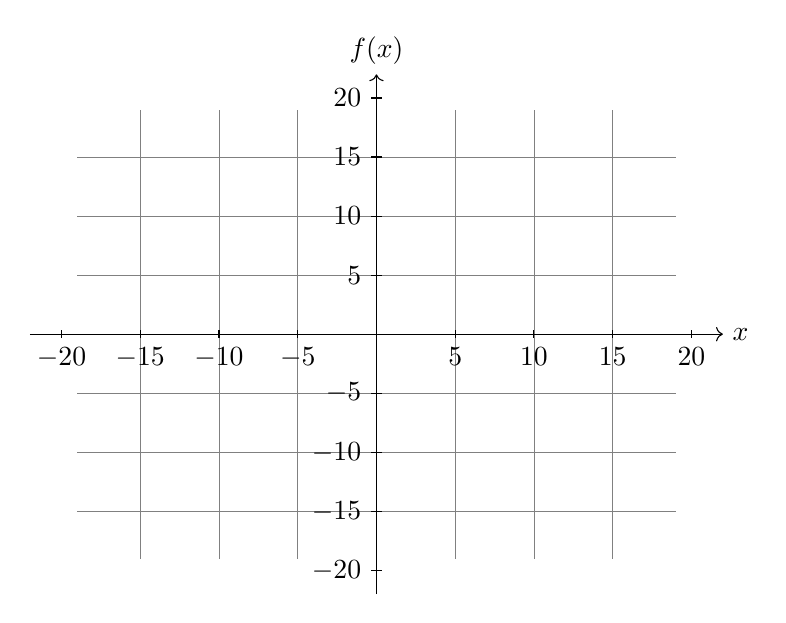
\begin{tikzpicture}[xscale=0.2,yscale=0.15]
	\draw[step=5,gray,very thin] (-19,-19) grid (19,19);
  \draw[->] (-22,0) -- (22,0) node[right] {$x$};
  \draw[->] (0,-22) -- (0,22) node[above] {$f(x)$};
 \foreach \x/\xtext in {-20/-20, -15/-15, -10/-10, -5/-5, 0/ , 5/5, 10/10, 15/15, 20/20}
    \draw[shift={(\x,0)}] (0pt,10pt) -- (0pt,-10pt) node[below] {$\xtext$};
  \foreach \y/\ytext in {-20/-20, -15/-15, -10/-10, -5/-5, 0/ , 5/5, 10/10, 15/15, 20/20}
    \draw[shift={(0,\y)}] (10pt,0pt) -- (-10pt,0pt) node[left] {$\ytext$};
\end{tikzpicture}
\end{center}
\noindent On this system of axes known as a Cartesian system (after R. Descartes) we plot the function itself. As a first example we come back to the function $f$ defined in (\ref{first_func}): $f(x)= 2x + 7$. Every $x$ is mapped to $2x + 7$. So for instance $3$ is mapped to $13$ (because $2\times 3 + 7 = 6+7=13$). We therefore mark the point $\left(3,13\right)$\footnote{The notation $\left( a,b \right)$ means the point whose horizontal and vertical components are $a$ and $b$, respectively. The point $\left( 0,0 \right)$ is often called the "`\textbf{origin}"'.}:
\begin{center}
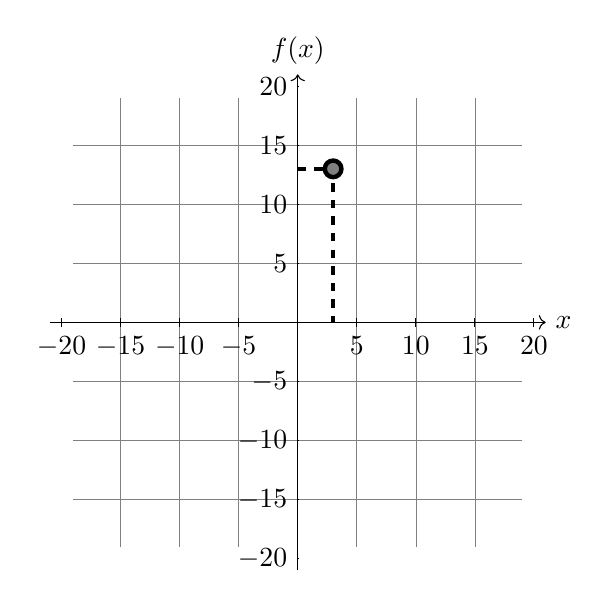
\begin{tikzpicture}[scale=0.15]
  \draw[step=5,gray,very thin] (-19,-19) grid (19,19);
	\draw[->] (-21,0) -- (21,0) node[right] {$x$};
  \draw[->] (0,-21) -- (0,21) node[above] {$f(x)$};
	\draw[dashed,ultra thick] (0,13) -- (3,13)--(3,0);
	\draw [black, fill=gray, ultra thick] (3,13) circle [radius=20pt];
 \foreach \x/\xtext in {-20/-20, -15/-15, -10/-10, -5/-5, 0/ , 5/5, 10/10, 15/15, 20/20}
    \draw[shift={(\x,0)}] (0pt,10pt) -- (0pt,-10pt) node[below] {$\xtext$};
  \foreach \y/\ytext in {-20/-20, -15/-15, -10/-10, -5/-5, 0/ , 5/5, 10/10, 15/15, 20/20}
    \draw[shift={(0,\y)}] (2pt,0pt) -- (-2pt,0pt) node[left] {$\ytext$};
\end{tikzpicture}
\end{center}
\noindent The dashed lines were added to emphasize that the point $\left( 3,13 \right)$ corresponds to $3$ on the horizontal axis and $13$ on the vertical one. We call them the horizontal and vertical components of the point $\left( 3,13 \right)$. We now add some other points related by the function $f$: $\left( 0,7 \right)$, $\left( 6,19 \right)$ and $\left( -5,-3 \right)$:
\begin{center}
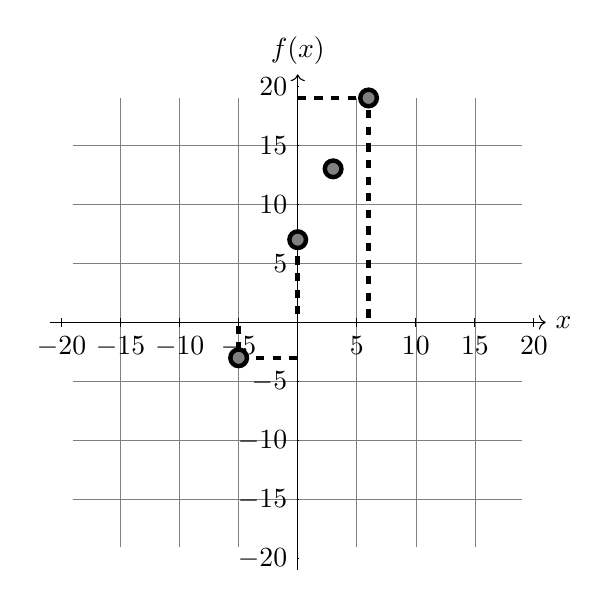
\begin{tikzpicture}[scale=0.15]
\draw[step=5,gray,very thin] (-19,-19) grid (19,19);
  \draw[->] (-21,0) -- (21,0) node[right] {$x$};
  \draw[->] (0,-21) -- (0,21) node[above] {$f(x)$};
	\draw[dashed,ultra thick] (0,7) -- (0,0);
	\draw[dashed,ultra thick] (0,19) -- (6,19)--(6,0);
	\draw[dashed,ultra thick] (0,-3) -- (-5,-3)--(-5,0);
	
	\draw [black, fill=gray, ultra thick] (3,13) circle [radius=20pt];
	\draw [black, fill=gray, ultra thick] (0,7) circle [radius=20pt];
	\draw [black, fill=gray, ultra thick] (-5,-3) circle [radius=20pt];
	\draw [black, fill=gray, ultra thick] (6,19) circle [radius=20pt];

 \foreach \x/\xtext in {-20/-20, -15/-15, -10/-10, -5/-5, 0/ , 5/5, 10/10, 15/15, 20/20}
    \draw[shift={(\x,0)}] (0pt,10pt) -- (0pt,-10pt) node[below] {$\xtext$};

  \foreach \y/\ytext in {-20/-20, -15/-15, -10/-10, -5/-5, 0/ , 5/5, 10/10, 15/15, 20/20}
    \draw[shift={(0,\y)}] (2pt,0pt) -- (-2pt,0pt) node[left] {$\ytext$};
\end{tikzpicture}
\end{center}
\noindent By drawing all the points $\left(x,f(x)\right)$ for all the values $x$ is allowed to take (in this case we implicitly assumed that the domain is $\mathbb{R}$), we get the \textbf{graph} of the function $f$:
\begin{center}
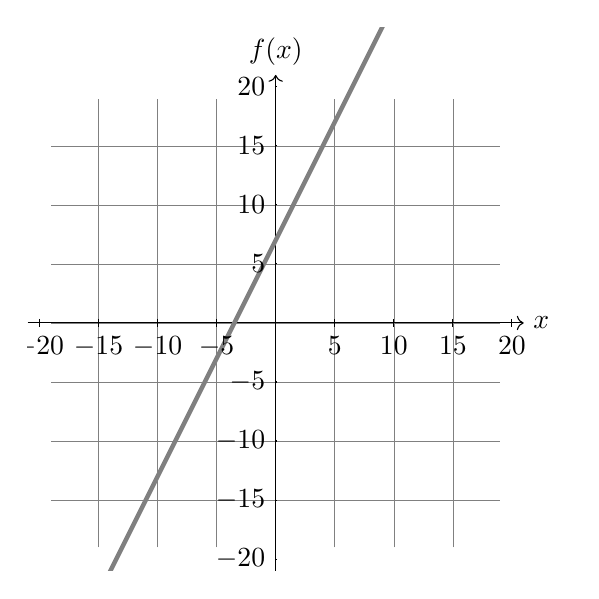
\begin{tikzpicture}[scale=0.15]
	\draw[step=5,gray,very thin] (-19,-19) grid (19,19);
	\clip (-21,-21) rectangle (25,25);
  \draw[->] (-21,0) -- (21,0) node[right] {$x$};
  \draw[->] (0,-21) -- (0,21) node[above] {$f(x)$};
	\draw[gray, ultra thick, domain=-20:20] plot (\x, {2*\x+7});
	
 \foreach \x/\xtext in {-20/-20, -15/-15, -10/-10, -5/-5, 0/ , 5/5, 10/10, 15/15, 20/20}
    \draw[shift={(\x,0)}] (0pt,10pt) -- (0pt,-10pt) node[below] {$\xtext$};

  \foreach \y/\ytext in {-20/-20, -15/-15, -10/-10, -5/-5, 0/ , 5/5, 10/10, 15/15, 20/20}
    \draw[shift={(0,\y)}] (2pt,0pt) -- (-2pt,0pt) node[left] {$\ytext$};
\end{tikzpicture}
\end{center}
\noindent Functions represented by a single straight line are called \textbf{linear}\footnote{Unlike physicists, mathematicians often add the condition of the graph having to pass through $\left( 0,0 \right)$ in order to call the function linear.}. Functions $g$ and $h$ defined in (\ref{FuncG}) and (\ref{FuncH}) are both non-linear and have the following graphs:
\begin{center}
	%graph of g
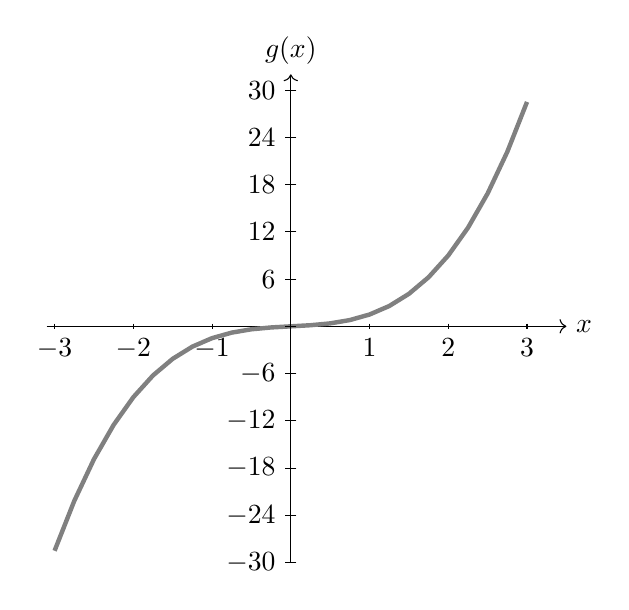
\begin{tikzpicture}[xscale=1, yscale = 0.1]
	
	%\draw[step=5,gray,very thin] (-3,-29) grid (3.4,31);
	\draw[->] (-3.1,0) -- (3.5,0) node[right] {$x$};
  \draw[->] (0,-30) -- (0,32) node[above] {$g(x)$};
	\draw[gray, ultra thick, domain=-3:3] plot (\x, {(\x*\x*\x +\x*0.5});
	
 \foreach \x/\xtext in { -3/-3,-2/-2, -1/-1, 0/ , 1/1, 2/2, 3/3 }
    \draw[shift={(\x,0)}] (0pt,10pt) -- (0pt,-10pt) node[below] {$\xtext$};

  \foreach \y/\ytext in {-30/-30, -24/-24, -18/-18, -12/-12, -6/-6, 0/ , 6/6, 12/12, 18/18, 24/24, 30/30}
    \draw[shift={(0,\y)}] (2pt,0pt) -- (-2pt,0pt) node[left] {$\ytext$};
	
\end{tikzpicture}
%graph of h
\begin{tikzpicture}[xscale = 5,yscale=6]
%\draw[step=5,gray,very thin] (-0.1,0.1) grid (1.1,1.1);
	\draw[->]  (0,-0.1)--(0,1.1);
	\draw[->]  (-0.1,0)--(1.1,0);
	\node [right] at (1.1,0) {$x$};
	\node [above] at (0,1.1) {$h(x)$};
	\draw[blue, ultra thick] (0,0) -- (0.5,0);
	\draw[blue, ultra thick] (0.5,1) -- (1,1);
	 \draw[blue, very thick](0.5, 0) circle (0.3mm);
	\filldraw [blue] (0.5,1) circle (0.3mm);
	
 \foreach \x/\xtext in {0/, 0.2/0.2, 0.4/0.4, 0.6/0.6, 0.8/0.8 , 1/1}
    \draw[shift={(\x,0)}] (0pt,0.3pt) -- (0pt,-0.3pt) node[below] {$\xtext$};

 \foreach \y/\ytext in {0/, 0.2/0.2, 0.4/0.4, 0.6/0.6, 0.8/0.8 , 1/1}
    \draw[shift={(0,\y)}] (0.3pt,0pt) -- (-0.3pt,-0pt) node[left] {$\ytext$};
	
\end{tikzpicture}
\end{center}
\noindent The vertical axis of the graph of $g$ (on the left) is "`zoomed in"' to fit on the page. Therefore, keep in mind that the part of the vertical axis shown represents a line $10$ times longer than the horizontal axis\footnote{This is not uncommon, so make sure to always look at the units of the axes.}. On the right we plot the graph of $h$. As long as $x<\frac{1}{2}$ the value of $h$ equals $0$. At $x=\frac{1}{2}$ the value of $h$ is \textbf{not} $0$ but $1$ which is emphasized by the hollow circle at $\left( \frac{1}{2},0 \right)$ and the filled circle at $\left( \frac{1}{2},1 \right)$. From $x=\frac{1}{2}$ onwards $h$ has the value $1$.

\subsection{Be a little implicit}

\noindent In section \ref{Expl_Func} we saw that one way of representing a function is to explicitly write out its action on its argument. An example of this is
\begin{equation}
\label{cubicExamp}
f(x) = x^5
\end{equation}
\noindent This is nothing but saying that we plug in any real number $x$ into the function $f$ and out comes its fifth power. The corresponding graph is\footnote{ Note once again that the vertical axis is "`zoomed out"' compared to the horizontal axis.}:
\begin{center}
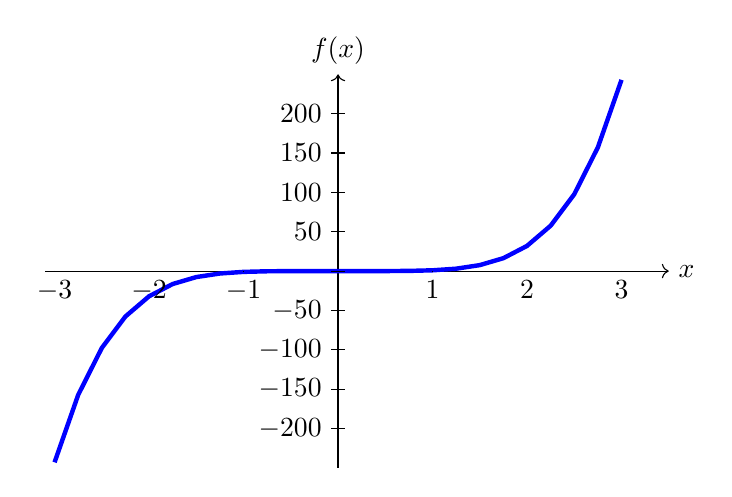
\begin{tikzpicture}[xscale=1.2, yscale = 0.01]
	
%	\clip (-21,-1100) rectangle (24,1200);

	\draw[->] (-3.1,0) -- (3.5,0) node[right] {$x$};
  \draw[->] (0,-250) -- (0,250) node[above] {$f(x)$};
	\draw[blue, ultra thick, domain=-3:3] plot (\x, {(\x*\x*\x*\x*\x});
	
 \foreach \x/\xtext in { -3/-3, -2/-2, -1/-1, 0/ , 1/1, 2/2, 3/3 }
    \draw[shift={(\x,0)}] (0pt,10pt) -- (0pt,-10pt) node[below] {$\xtext$};

  \foreach \y/\ytext in { -200/-200, -150/-150, -100/-100, -50/-50,  0/ , 50/50, 100/100, 150/150, 200/200}
    \draw[shift={(0,\y)}] (2pt,0pt) -- (-2pt,0pt) node[left] {$\ytext$};
	
\end{tikzpicture}
\end{center}
\noindent This same graph can be gotten in a slightly different way. We consider all points of the form $\left( x,y \right)$ that obey the condition
\begin{equation}
\label{ImplNotation}
y-x^5 = 0
\end{equation}
We compare the set of points obeying equation (\ref{cubicExamp}) with the set of points obeying equation (\ref{ImplNotation}). They are of course the same:
$$
\left\{ \left(x,f(x)\right)| f(x) = x^5  \right\} = \left\{ \left( x,y \right) | y - x^5 = 0 \right\}
$$
Plotting these 2 sets on a Cartesian system as above would give exactly the same graph. The representation on the left is known as the explicit representation of the function while the one on the right is its implicit representation. You may say that calling these a "`different"' representation is a bit of a stretch. We did not actually change anything. We only
\begin{enumerate}
\item changed the name of the function from $f$ to $y$.
\item omitted the argument of $y$.
\item replaced the condition $y = x^5$ by $y - x^5 = 0$.
\end{enumerate}
\noindent None of these actually changes anything. We are indeed allowed to rename the function and omit the explicit mention of its argument. The third action amounts to subtracting $x^5$ from both the LHS and the RHS\footnote{Subtracting the same value from both sides of an equation does not change it. If it is true that $a = b$ than it also has to be true that $a-c=b-c$ not matter what the value of $c$ is.}. We still consider all the points of the form $\left(a,b\right)$ where the value of $b$ equals $a^5$.\\

\noindent The main difference is the way we think about the points on the graph. In the \textbf{explicit} representation a vertical component is determined for every value in the domain. By definition an explicit equation is of the form $y=f(x)$ such that on the LHS only $y$ appears (no $y^2$ for instance) and on the RHS there is no mention of $y$. While in the \textbf{implicit} representation we think of the graph as all the points $(x,y)$ obeying some condition. Of course, if a point $\left( x,y\right)$ obeys the relation $y-x^5=0$, then it clearly also obeys $y = x^5$. This should not be surprising as both represent the same thing. There are nevertheless many examples where going from the implicit to the explicit representation is not as straightforward as it may seem at first sight and it is often even impossible. Let us consider two examples: 
\begin{enumerate}
\item The implicit equation
$$
y^3 -2 x + 5 = 0
$$
can be rewritten in explicit form as
$$
y(x) = \sqrt[3]{2x - 5} 
$$
\item The implicit equation 
$$
3y^{19} - 4y^2 +17x^3 -2x +6 = 0
$$
can not be written in the form form $y(x) = f(x)$ where the RHS does not contain any $y$. Try as you may, you will not be able to find an explicit equation representing this function\footnote{In many cases the "`function"' gotten from an implicit equation is not a function strictly speaking. It does not obey the definition of what mathematicians call a function. But the exact definition is of no importance to us in this discussion. It remains true that the set of all points $x$ and $y$ obeying relations as described in the text can be drawn and can be used to describe physical quantities whether in the explicit or the implicit representation.}. 
\end{enumerate}

\subsection{Parametric representation}

\noindent The final representation of functions we discuss here is known as \textbf{parametrization}. Instead of thinking of $y$ as a function of $x$ as in section (\ref{Expl_Func}), we now think of both $x$ and $y$ as being dependent on some parameter $t$. In physical applications this $t$ may represent time but could in principle be any other parameter. The function is then written as $\left( x(t), y(t) \right)$. This probably sounds a bit abstract, so let us look at an example. We first choose the range of values that $t$ can take. For the sake of this example, we choose the parameter $t$ to be in $\left[ 0,16 \right]$ and define the function as
\begin{equation}
\label{ParamExamp}
\left\{
\begin{array}{ll}
 x(t) = \frac{t}{2} \\\\
y(t) = t^2 
\end{array}
\right. 
\end{equation}
Both $x$ and $y$ are functions of $t$. For every value of $t$, a value for both $x$ and $y$ is determined from (\ref{ParamExamp}). For instance, for $t=0$ we find $x(0) = 0$ and $y(0)=0$ so that we mark the point $\left( 0,0 \right)$ on the graph. And for $t=3$ we have $x(3)=1,5$ and $y(3)=9$, therefore we mark $\left( 1,5 ; 9 \right)$. If we do this for all values of $t$ in $\left[ 0,16 \right]$ and plot all the points we find the graph of this function:
\begin{center}
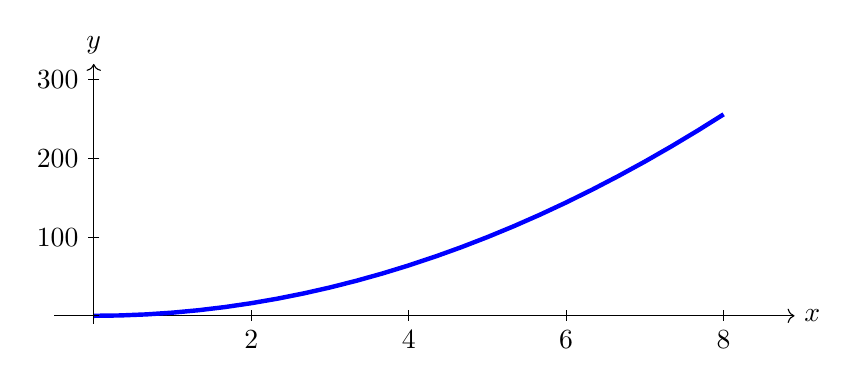
\begin{tikzpicture}[xscale=1,yscale=0.01]
	
  \draw[->] (-0.5,0) -- (8.9,0) node[right] {$x$};
  \draw[->] (0,-10) -- (0,320) node[above] {$y$};
	\draw[blue, ultra thick, domain=0:8] plot (\x, {4*\x*\x});
	
 \foreach \x/\xtext in {0/, 2/2, 4/4, 6/6, 8/8 }
    \draw[shift={(\x,0)}] (0pt,200pt) -- (0pt,-200pt) node[below] {$\xtext$};

  \foreach \y/\ytext in {0/ , 100/100, 200/200, 300/300}
    \draw[shift={(0,\y)}] (2pt,0pt) -- (-2pt,0pt) node[left] {$\ytext$};
\end{tikzpicture}
\end{center}
\noindent This does not look very different from the plots of the functions we discussed above. But the parametric representation allows for a wide range of figures that are impossible to write out in explicit form. Here are a couple of examples:
\begin{center}
\begin{tikzpicture}[scale=0.2]
\draw[domain=1:14,samples = 5000,smooth, blue, very thick] plot[parametric,id=spiral-diagonal] function{(2*t) + (2*cos(14*t)) + (1/t),(2*t) + (2*sin(15*t)) + (1/t)};
\draw[->] (-0.1,0) -- (30,0) node[right] {$x$};
\draw[->] (0,-0.1) -- (0,30) node[above] {$y$};
\end{tikzpicture}
\begin{tikzpicture}[scale=0.6]
\draw[domain=-8:8,samples = 1000,smooth, blue, very thick] plot[parametric,id=dream-catcher] function{6*sin(11.92*t)*cos(cos(18.5*t)),6*cos(11.92*t)*cos(11.92*t)*cos(11.92*t)*cos(11.92*t)*sin(sin(18.5*t))};
\draw[->] (-6.5,0) -- (6.5,0) node[right] {$x$};
\draw[->] (0,-6) -- (0,6) node[above] {$y$};
\end{tikzpicture}
\end{center}
\begin{center}
\begin{tikzpicture}[scale=0.2]
\draw[domain=0:2*pi,samples = 1000,smooth, red, ultra thick] plot[parametric,id=heart] function{16*sin(t)*sin(t)*sin(t),13*cos(t)-5*cos(2*t)-2*cos(3*t)-cos(4*t)};
\draw[->] (-18,0) -- (18,0) node[right] {$x$};
\draw[->] (0,-19) -- (0,12) node[above] {$y$};
\end{tikzpicture}
\end{center}
\noindent The exact equations $x(t)$ and $y(t)$ for each of these are of no importance to us. These examples were "`borrowed"' by yours truly from Google with the sole purpose of showing the versatility of this representation. The red color in the bottom figure is only there for romantic reasons.

\subsection{A graph says more than a thousand symbols}
\label{GraphsExamps}
\noindent Below are the graphs of some common functions which play important roles in physics and we will get acquainted with them in due time. 
\begin{center}
\begin{tikzpicture}[xscale=0.3,yscale=1.5]
	\draw[->]  (-10,0)--(10,0);
	\draw[->]  (0,-1.1)--(0,1.1);
	\node [right] at (10.5,0) {$x$};
	\node [above] at (0,1.1) {$\sin(x)$};
	\draw[smooth, domain = -10:10, blue, ultra thick] plot function{sin(x)};
	
 \foreach \x/\xtext in {-10/-10, -5/-5, 0/ , 5/5, 10/10}
    \draw[shift={(\x,0)}] (0pt,0.3pt) -- (0pt,-0.3pt) node[below] {$\xtext$};

 \foreach \y/\ytext in {-1/-1, -0.5/-0.5, 0/ , 0.5/0.5, 1/1}
    \draw[shift={(0,\y)}] (0.3pt,0pt) -- (-0.3pt,-0pt) node[left] {$\ytext$};
	\node[align=center,font=\bfseries, yshift=1.5em] (title) at (current bounding box.north){Sine};
	
\end{tikzpicture}
\begin{tikzpicture}[xscale=1,yscale=0.02]
	\draw[->]  (-1,0)--(5,0);
	\draw[->]  (0,-5)--(0,150);
	\node [right] at (5.1,0) {$x$};
	\node [above] at (0,160) {$e^x$};
	\draw[smooth, domain = -1:5, blue, ultra thick] plot function{exp(x)};
	
 \foreach \x/\xtext in {-1/-1, 0/ , 1/1, 3/3, 5/5}
  \draw[shift={(\x,0)}] (0pt,10pt) -- (0pt,-10pt) node[below] {$\xtext$};

 \foreach \y/\ytext in {0/ ,30/30, 60/60, 90/90, 120/120, 150/150}
    \draw[shift={(0,\y)}] (0.3pt,0pt) -- (-0.3pt,-0pt) node[left] {$\ytext$};
	\node[align=center,font=\bfseries, yshift=1.5em] (title) at (current bounding box.north){Exponential};
\end{tikzpicture}
\end{center}
\begin{center}
\begin{tikzpicture}[xscale=1.5,yscale=0.08]

	\draw[->]  (-2.1,0)--(2.2,0);
	\draw[->]  (0,-30)--(0,28);
	\node [right] at (2.3,0) {$x$};
	\node [above] at (0,31) {$1/x$};
	\draw[smooth, domain = -2:-0.035, blue, ultra thick,samples=100] plot function{1/x};
	\draw[smooth, domain = 0.035:2.1, blue, ultra thick,samples=100] plot function{1/x};
	
 \foreach \x/\xtext in {-2/-2, -1.5/-1.5, -1/-1, -0.5/-0.5, 0/ , 0.5/0.5, 1/1, 1.5/1.5, 2/2}
  \draw[shift={(\x,0)}] (0pt,10pt) -- (0pt,-10pt) node[below] {$\xtext$};

 \foreach \y/\ytext in {-30/-30,-20/-20, -10/-10 , 0/ , 10/10, 20/20, 30/30}
    \draw[shift={(0,\y)}] (1pt,0pt) -- (-1pt,0pt) node[left] {$\ytext$};

\node[align=center,font=\bfseries, yshift=1.5em] (title) at (current bounding box.north){Hyperbola};			
\end{tikzpicture}
\begin{tikzpicture}[scale=0.2]

	\draw[->]  (-11,0)--(11,0);
	\draw[->]  (0,-11)--(0,11);
	\node [right] at (11,0) {$x$};
	\node [above] at (0,11) {$id(x)$};
	\draw[smooth, domain = -10:10.2, blue, ultra thick,samples=500] plot function{x};
	
 \foreach \x/\xtext in {-10/-10, -5/-5, 0/ , 5/5, 10/10}
  \draw[shift={(\x,0)}] (0pt,10pt) -- (0pt,-10pt) node[below] {$\xtext$};

 \foreach \y/\ytext in {-10/-10, -5/-5, 0/ , 5/5, 10/10}
    \draw[shift={(0,\y)}] (10pt,0pt) -- (-10pt,0pt) node[left] {$\ytext$};
	
	\node[align=center,font=\bfseries, yshift=1.5em] (title) at (current bounding box.north){Identity};
	
\end{tikzpicture}
\end{center}
\begin{center}
\begin{tikzpicture}[xscale = 0.5,yscale = 0.5]

	\draw[->]  (-6,0)--(6,0);
	\draw[->]  (0,-5)--(0,5);
	\draw[smooth, domain = -5.8:-4.9, blue, ultra thick,samples=100] plot function{tan(x)};
	\draw[smooth, domain = -4.52:-1.76, blue, ultra thick,samples=100] plot function{tan(x)};
\draw[smooth, domain = -1.38:1.38, blue, ultra thick,samples=100] plot function{tan(x)};
	\draw[smooth, domain = 1.76:4.52, blue, ultra thick,samples=100] plot function{tan(x)};
	\draw[smooth, domain = 4.9:5.8, blue, ultra thick,samples=100] plot function{tan(x)};
	\draw[dashed, thin] (1.57,-5.2) -- (1.57,5.2);
	\draw[dashed, thin] (-1.57,-5.2) -- (-1.57,5.2);
	\draw[dashed, thin] (4.71,-5.2) -- (4.71,5.2);
	\draw[dashed, thin] (-4.71,-5.2) -- (-4.71,5.2);
	\node [right] at (6.3,0) {$x$};
	\node [above] at (0,5.3) {$tan(x)$};
	
 \foreach \x/\xtext in {-4/-4, -2/-2, 0/ , 2/2, 4/4}
  \draw[shift={(\x,0)}] (0pt,10pt) -- (0pt,-10pt) node[below] {$\xtext$};
	\foreach \x/\xtext in {-5/ , -3/, -1/ , 1/, 3/ ,5/ }
  \draw[shift={(\x,0)}] (0pt,3pt) -- (0pt,-3pt) node[below] {$\xtext$};

 \foreach \y/\ytext in {-4/-4, -2/-2, 0/ , 2/2, 4/4}
 \draw[shift={(0,\y)}] (10pt,0pt) -- (-10pt,0pt) node[left] {$\ytext$};
 \foreach \y/\ytext in {-3/ , -1/ , 1/1, 3/ }
 \draw[shift={(0,\y)}] (3pt,0pt) -- (-3pt,0pt) node[left] {$\ytext$};
	
\node[align=center,font=\bfseries, yshift=1.5em] (title) at (current bounding box.north){Tangent};

\end{tikzpicture}
\begin{tikzpicture}[xscale=0.3, yscale = 0.04]

	\draw[->]  (-11,0)--(11,0);
	\draw[->]  (0,-10)--(0,110);
	\node [right] at (11,0) {$x$};
	\node [above] at (0,110) {$x^2$};
	\draw[smooth, domain = -10:10, blue, ultra thick,samples=500] plot function{x*x};
	
 \foreach \x/\xtext in {-10/-10, -5/-5, 0/ , 5/5, 10/10}
  \draw[shift={(\x,0)}] (0pt,10pt) -- (0pt,-10pt) node[below] {$\xtext$};

 \foreach \y/\ytext in {0/ , 50/50, 100/100}
    \draw[shift={(0,\y)}] (10pt,0pt) -- (-10pt,0pt) node[left] {$\ytext$};
	
	\node[align=center,font=\bfseries, yshift=1.5em] (title) 
    at (current bounding box.north)
    {Parabola};
	
\end{tikzpicture}
\end{center}

\section{Solving equations}
\label{EqSolveBasics}
\subsection{Basic operations on equations}
\noindent An equation is an expression of the form
\begin{equation}
\label{IntroEquations}
f(x) = g(x)
\end{equation}
with both $f$ and $g$ functions. This equation can be interpreted in 2 different ways:
\begin{enumerate}[i]
\item A statement of truth: "`$f$ and $g$ are equal"'. Equation (\ref{IntroEquations}) tells us in this interpretation that the functions $f$ and $g$ give the same output for all values of $x$.
\item A condition that needs to be met. Equation (\ref{IntroEquations}) tells us in this interpretation that we are looking for all values of $x$ for which $f$ and $g$ give the same result. As we will see below, depending on the functions $f$ and $g$ there may be a single value of $x$ where this is the case, there may be multiple values (even infinitely many) or none at all.
\end{enumerate}
\noindent The context should always make it clear which of the 2 interpretations is being used. In the rest of this chapter we will focus on the second interpretation.\\

\noindent "`Solving"' equation (\ref{IntroEquations}) means finding those values of $x$ for which the equality holds. We start with an equation that has a very obvious solution:
\begin{equation}
3x +2 = 17
\label{ValEquation}
\end{equation}
By staring at this equation for a moment you probably realize that the value that $x$ has to take for it to hold true is $x=5$. Indeed, $3 \times 5 + 2 = 17$. But staring and hoping is only one of a wide variety of techniques for solving equations.\\

\noindent The most basic of techniques is isolating the variable $x$ on one side of the equality sign. We start by subtracting $2$ from both the LHS and the RHS of (\ref{ValEquation}):
$$
 3x + 2 - 2   =  17 - 2
$$
which leaves us with
$$
3x = 15
$$
Before continuing with solving equation (\ref{ValEquation}) I want to dwell just a bit longer on this subtraction. Why are we allowed to do it?\\

\subsubsection{Intermezzo: Manipulating equations}
\noindent Well, think of it this way. It is of course true that $11=11$. Adding $8$ to both sides will not make it false. It is indeed also true that $11+8 = 11+8$ which often goes through life as $19=19$. Adding the same number to both sides of an equation does not alter its validity. This is also true when subtracting, multiplying with and dividing by the same number on both sides of the equation (except for dividing both sides by $0$ which we are not allowed to do anyway).\\ 

\noindent  In mathematician's lingo this is expressed in the following way: $\forall a, b$ and $c \in \mathbb{R}$:
\begin{eqnarray}
\label{LogStatement} a = b & \Leftrightarrow & a + c = b + c \\
a = b & \Leftrightarrow & a - c = b - c \\
a = b & \Leftrightarrow & a \times c = b \times c \\
\label{divExamp} a = b & \Leftrightarrow & \frac{a}{c} = \frac{b}{c}
\end{eqnarray}
\noindent The symbol $\forall$ is read as "for each" and the colon as "such that". The arrow $\Leftrightarrow$ is read as "if and only if" or also as "`is equivalent with"' and means that if the statement to its right is true then the statement to its left also has to be true and vice versa\footnote{The arrow $\Leftrightarrow$ is actually a combination of $\Rightarrow$ and $\Leftarrow$. We consider 2 logical statements $p$ and $q$ that may or may not be true, for instance "`Brussels is a city in Argentina"'. Note that for a statement to be logical it need not be true though its truth needs to be objectively decidable. The statement "`sour is better than bitter"' is not a logical statement as there is no objective measure to determine its truth. The statement $p \Rightarrow q$ is read as "$p$ implies $q$" and means that if $p$ is true then $q$ also has to be true, but not necessarily the other way around. While $p \Leftarrow q$ means that if $q$ is true, then $p$ has to be true, though not necessarily the other way around.}. Statement (\ref{LogStatement}) in words is "if the numbers $a$ and $b$ are equal, then we can add to both any number $c$ and they still remain equal, no matter the values of $a$, $b$ or $c$, and vice versa". As mentioned above, for (\ref{divExamp}) we also need the additional condition that $c \neq 0$. All these statement above basically say that applying any of the 4 basic arithmetic operations to both sides of an equation does not alter its validity (i.e. if the statement was true before, it remains true and if it was false it remains false). This means that if $f(x) = g(x)$ for some value of $x$, then $f(x) - c = g(x) - c$. This is what we did as a first step towards solving equation (\ref{ValEquation}).\\
 
\noindent You may think "I am allowed to do anything with equations as long as I do the same thing on both sides". This seems appealing, but it is wrong. Take for instance the equality $(4)^2 = (-4)^2$ which is true as both sides are equal to $16$. But $4 = \sqrt{(4)^2} \neq \sqrt{(-4)^2} = -4$. Taking the square root of both sides of an equation can indeed turn a true statement into a false one. Though we are not allowed to take the square root of both sides of an equation, we are allowed to take the square of the equation without altering its validity.\\

\noindent The combination of these two last properties is mathematically summarized as follows:
\begin{eqnarray*}
\forall a,b \in \mathbb{R}:a = b & \Rightarrow & a^2 = b^2
\end{eqnarray*}
Notice that the implication is only valid in one direction here. 

\subsubsection{Back to solving equations}

Coming back to solving that equation, we continue by dividing both sides by $3$:
$$
\frac{3x}{3} = \frac{15}{3}
$$
so that we finally find
$$
x = 5
$$
By isolating the variable on one side of the equality we solved the equation, finding the same (and only) solution as by the old "`stare and hope"' method above.\\

\subsection{Graphical interpretation of solutions}

\noindent What does it mean when we say "$x_1$ is a solution of the equation $f(x) = 0$"? It means that if we plug in the value $x_1$ into the function $f$ the output will be $0$. In other words, $\left( x_1, 0 \right)$ is on the graph of the function $f$. Or still, the graph of the function $f$ coincides with the horizontal axis (usually called the x-axis) at $x = x_1$. Below is the graph of $f(x) = x^3 - 4 x^2 + 3$
\begin{center}
\begin{tikzpicture}[xscale=1, yscale = 0.2]

	\draw[->]  (-2,0)--(5,0);
	\draw[->]  (0,-10)--(0,30);
	\node [right] at (5.5,0) {$x$};
	\node [above] at (0,30) {$f(x)$};
	\draw[smooth, domain = -1.5:5, blue, ultra thick,samples=300] plot function{(x*x*x) - (4*x*x) + 3};
	
 \foreach \x/\xtext in {-1/-1, 1/1, 3/3 , 5/5}
  \draw[shift={(\x,0)}] (0pt,10pt) -- (0pt,-10pt) node[below] {$\xtext$};

 \foreach \y/\ytext in {-5/-5, 5/5, 15/15, 25/25}
    \draw[shift={(0,\y)}] (5pt,0pt) -- (-5pt,0pt) node[left] {$\ytext$};
		
\end{tikzpicture}
\end{center}
The solutions of the equation
$$
f(x) = x^3 - 4x^2 + 3 = 0
$$
are the values of $x$ at which the graph coincides with the $x$-axis. Just by looking at the graph, it seems one of the solutions is at $x=1$. But looking is not enough. The solution could be very close to $x=1$, maybe at $x=1,0001$, so that we cannot determine its exact value visually. To confirm that $x=1$ is indeed a solution we plug it into the function $f$ and find indeed that $f(1)=0$. The  two other solutions of the equation seem to be a bit above $x=-1$ and just under $x=4$. The exact values of the solutions can be found in this case by a method we will discuss further in the text. But it will often be impossible to determine the exact value of the solutions. There are nevertheless techniques to find approximate values for the solutions which is sufficient for many physical applications. More on this later.

\section{Polynomial functions}

\noindent One type of function that pops up everywhere in science, and with good though non-trivial reasons, is called a polynomial function. Examples are:
\begin{eqnarray*}
 f(x) & = & x^4 +5x \\
f(x) & = & 3x^{25} + \frac{4}{7}x^{13} - 9x^8 \\
f(x) & = & -4 \\
f(x) & = & x^2 - 15
\end{eqnarray*}
\noindent What all of these have in common is their basic structure:
\begin{equation}
\label{Def_Polynom}
f(x) = a_n x^n + a_{n-1} x^{n-1} + a_{n-2} x^{n-2} + \cdots + a_2 x^2 + a_1 x^1 + a_0 = \sum\limits_{i=0}^{n} a_i \; x^{i}
\end{equation}
All of the $a_i$'s are real numbers and $n$ is a natural number. Polynomial functions are always of the form "`a number $a_n$ times the $n^{th}$ power of $x$ plus a second constant $a_{n-1}$ times the $(n-1)^{th}$ power of $x$ plus... until an $n^{th}$ constant $a_1$ times $x^1$ (which is simply $x$ itself) plus a final constant $a_0$"'. For instance, if $n=3$, a possible polynomial function is 
$$
f(x) = 2 x^3 + 4x -3
$$ 
\noindent In this case
\begin{eqnarray*}
a_3 = 2 \\
a_2 = 0 \\
a_1 = 4 \\
a_0 = -3
\end{eqnarray*}
The highest exponent of $x$ appearing in the function is called the \textbf{degree} of the polynomial. The degrees of the 4 first polynomials above are: $4, 25, 0$ and $2$.\\

\noindent We will encounter in physics many equations of the form
\begin{equation}
\sum\limits_{i=0}^{n} a_i \: x^{i} = 0
\end{equation}
Such statements are known as polynomial equations. Solving these is among the basic skills necessary to do physics.

\subsection{$1^{st}$ degree polynomials}

\noindent A $1^{st}$ degree polynomial function has the generic form
\begin{equation}
f(x) = a_1 x + a_0
%\label{FirstOrdExampFunc}
\end{equation}
These are also known as linear functions\footnote{In most texts this will be written as $f(x) = a x + b$ with $a$ and $b$ real numbers.}. The graphs of such functions are straight lines. The meaning of $a_1$ and $a_0$ can be seen on the graphs below. 
\begin{center}
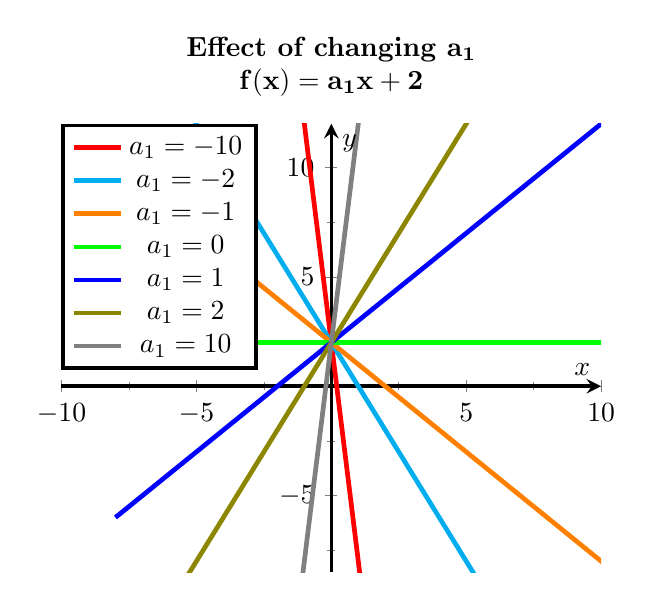
\begin{tikzpicture}
\begin{axis}
[
		minor tick num=1,
		axis x line=middle,
		line width = 1.3,
		align =center,
		title={\textbf{Effect of changing $\bf{a_1}$}\\ $\bf{f(x)= a_1 x +2}$},
		axis y line=middle,
		xmax=10, xmin=-10,
		ymax=12, ymin=-8.5,
		xlabel=$x$,ylabel=$y$,
		legend style={at={(0,1)},anchor=north west}
		%legend style={
			%	cells={anchor=east},
				%legend pos=outer north west
			%}
	]
\foreach \num / \col in {-10/red, -2/cyan, -1/orange, 0/green, 1/blue, 2/olive, 10/gray}  {
				\edef\temp{\noexpand\addplot[line width=1.7pt, samples=500, domain= -8:12, color= \col]
					{\num*x +2};}
        \temp
				 \addlegendentryexpanded{$a_1 = \num$};
}
\end{axis}
\end{tikzpicture}
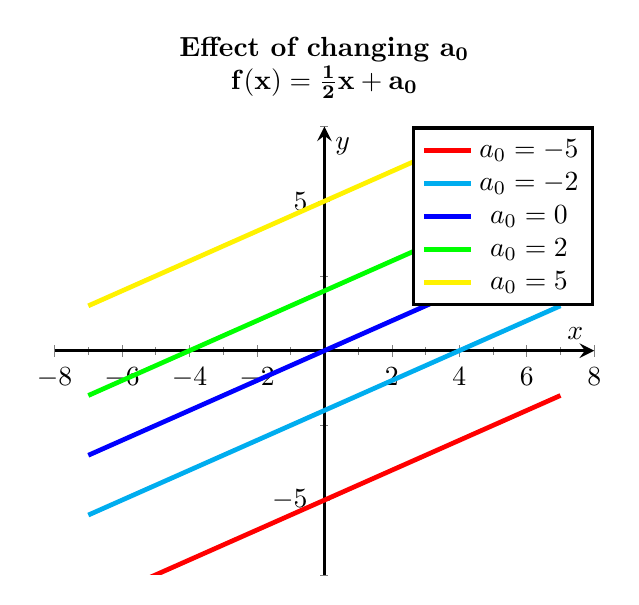
\begin{tikzpicture}
\begin{axis}
[
		minor tick num=1,
		axis x line=middle,
		line width = 1.3,
		align =center,
		title={\textbf{Effect of changing $\bf{a_0}$}\\ $\bf{f(x)= \frac{1}{2} x +a_0}$},
		axis y line=middle,
		xmax=8, xmin=-8,
		ymax=7.5, ymin=-7.5,
		xlabel=$x$,ylabel=$y$,
		legend style={at={(1,1)},anchor=north east}
	]
\foreach \num / \col in {-5/red, -2/cyan, 0/blue, 2/green, 5/yellow}  {
				\edef\temp{\noexpand\addplot[line width=1.7pt, samples=500, domain= -7:7, color= \col]
					{0.5*x +\num};}
        \temp
				 \addlegendentryexpanded{$a_0 = \num$};
}
\end{axis}
\end{tikzpicture}
\end{center}
\noindent The coefficient $a_1$ is a measure of the slope of the function and $a_0$ is the value at which the function crosses the $y$-axis.
\begin{itemize}
\item $\mathbf{a_1 > 0: }$ graph has \textbf{upward} slope (when read from left to right). As $a_1$ increases the upward slope becomes steeper.
\item $\mathbf{a_1 = 0: }$ horizontal graph (the green line on the left graph above, which is actually a $0^{th}$ order polynomial).
\item $\mathbf{a_1 < 0: }$ graph has \textbf{downward} slope (when read from left to right).
\end{itemize}
 
\subsubsection{Solving $1^{st}$ degree polynomial equations}

\noindent Remember that solving the linear equation
\begin{equation}
a_1 x + a_0 = 0
\label{FirstOrdExamp}
\end{equation}
means finding the value(s) of $x$ for which the equality holds. We explicitly assume that $a_1 \neq 0$ as the equation would not be a $1^{st}$ degree polynomial otherwise\footnote{If $a_1=0$ then the polynomial function is $f(x)= a_0$. This function maps any $x$ onto the number $a_0$. The graph is a horizontal line at $y=a_0$. The solution(s) of the equation $f(x) = a_0 = 0$ depend on the value of $a_0$. If $a_0 \neq 0$ then there are no solutions. And if $a_0=0$ than all values of $x$ are solutions.}. To solve equation (\ref{FirstOrdExamp}) the steps are
\begin{eqnarray*}
 & a_1 x + a_0  & = \;0 \\
 \Leftrightarrow & a_1 x &  = \;  - a_0 \\
  \Leftrightarrow & x  & =  \;- \frac{a_0}{a_1}
\end{eqnarray*}
\noindent In the first step we subtract $a_0$ from both sides and in the second step we divide both sides of the equation by $a_1$ (which is allowed as we know that $a_1 \neq 0$). The solution is thus $x = -\frac{a_0}{a_1}$.
\begin{center}

\begin{tabular}{ |ccc| }
  \hline
	& & \\
  $\bf{a_1 x + a_0 = 0}$ & $\bf{\Leftrightarrow}$ & $\bf{x =  - \frac{a_0}{a_1}}$ \\
  & & \\
	\hline
	\end{tabular}
\end{center}
\noindent Every $1^{st}$ degree polynomial equation has exactly $1$ solution given by $x = -\frac{a_0}{a_1}$. Equation (\ref{ValEquation}) is a $1^{st}$ degree polynomial equation: $3x + 2 = 17$. This is the same equation as $3x -15 = 0$. Its solution is therefore $x= - \frac{-15}{3} = 5$ which is indeed the solution we found before. Another example of a linear equation is $f(x)=-3x + 4$. The coefficients were $a_1 = -3$ and $a_0 = 4$ so that its solution is $-\frac{4}{-3} = \frac{4}{3} = 1.333\cdots$. Both solutions are highlighted in red circles below.
\begin{center}
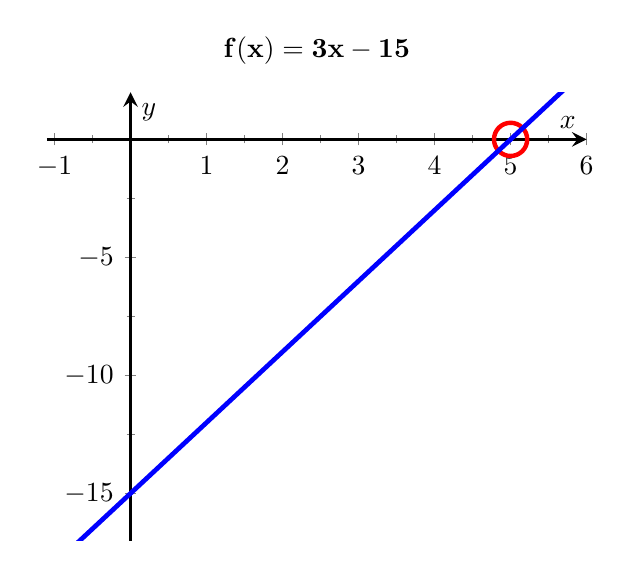
\begin{tikzpicture}
\begin{axis}
[
		minor tick num=1,
		axis x line=middle,
		line width = 1.3,
		title={$\bf{f(x)=3x -15}$},
		axis y line=middle,
		xmax=6, xmin=-1.1,
		ymax=2, ymin=-17,
		xlabel=$x$,ylabel=$y$,
	]
	\draw [red, ultra thick] (5,0) circle [radius=6pt];
%\draw [red, ultra thick] (4,0) circle [radius=6pt];
	\addplot[line width=1.7pt, samples=500, domain= -1.1:6, color= blue]
					{3*x -15};
\end{axis}
\end{tikzpicture}
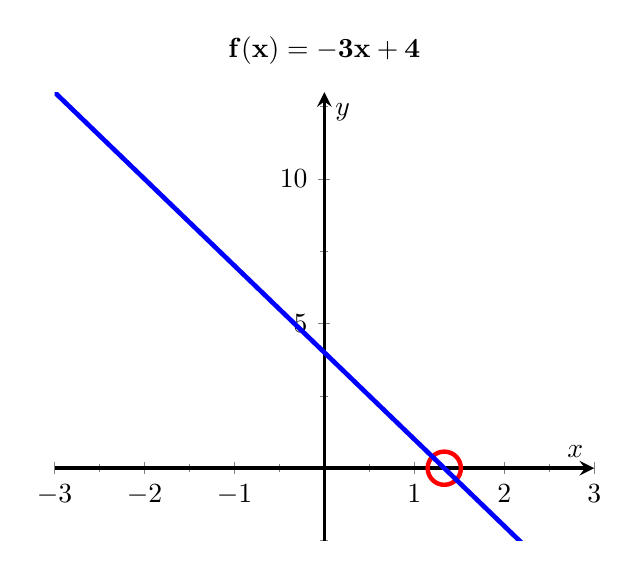
\begin{tikzpicture}
\begin{axis}
[
		minor tick num=1,
		axis x line=middle,
		line width = 1.3,
		title={$\bf{f(x)=-3x +4}$},
		axis y line=middle,
		xmax=3, xmin=-3,
		ymax=13, ymin=-2.5,
		xlabel=$x$,ylabel=$y$,
	]
	\draw [red, ultra thick] (1.333,0) circle [radius=6pt];
%\draw [red, ultra thick] (4,0) circle [radius=6pt];
	\addplot[line width=1.7pt, samples=500, domain= -3:3, color= blue]
					{-3*x +4};
\end{axis}
\end{tikzpicture}
\end{center}


\subsection{$2^{nd}$ degree polynomials}

\noindent A $2^{nd}$ degree polynomial function is of the form:
\begin{equation}
\label{QuadrEq}
f(x) = a_2 x^2 + a_1 x + a_0
\end{equation}
The corresponding graph is known as a parabola. Below are a couple of graphs to visualize the effect of changing each of the three coefficients $a_2, a_1$ and $a_0$ separately.
\begin{center}
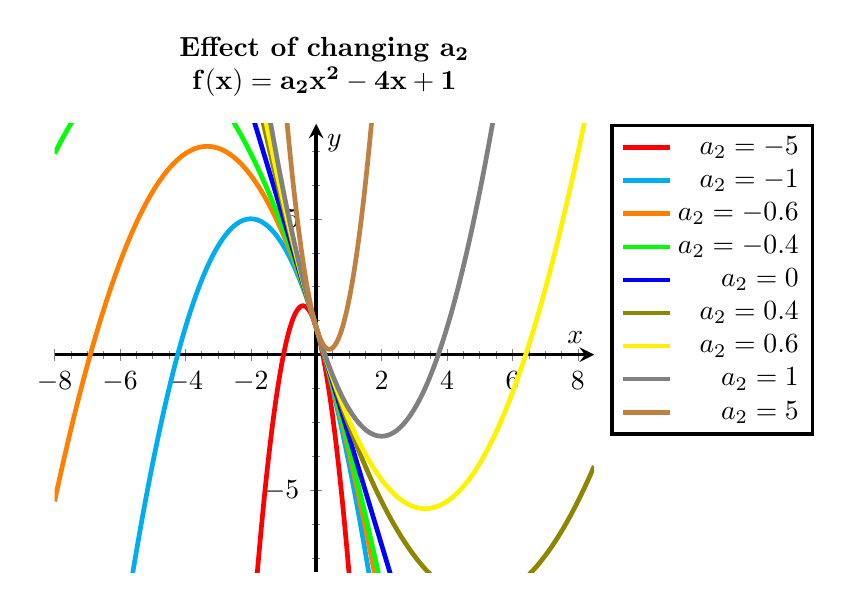
\begin{tikzpicture}
\begin{axis}
[
		minor tick num=3,
		axis x line=middle,
		line width = 1.3,
		align =center,
		title={\textbf{Effect of changing $\bf{a_2}$}\\ $\bf{f(x)=a_2 x^2 - 4x +1}$},
		%title={$\bf{f(x)=a_2 x^2 - 4x +1}$},
		axis y line=middle,
		xmax=8.5, xmin=-8,
		ymax=8.5, ymin=-8,
		xlabel=$x$,ylabel=$y$,
		legend style={
				cells={anchor=east},
				legend pos=outer north east
			}
	]
\foreach \num / \col in {-5/red, -1/cyan, -0.6/orange, -0.4/green, 0/blue, 0.4/olive, 0.6/yellow, 1/gray, 5/brown}  {
				\edef\temp{\noexpand\addplot[line width=1.7pt, samples=500, domain= -8:8.5, color= \col]
					{\num*x^2 - 4*x +1};}
        \temp
				 \addlegendentryexpanded{$a_2 = \num$};
}
\end{axis}
\end{tikzpicture}
\end{center}
\noindent Note the following points:
\begin{itemize}
\item As the absolute value of $a_2$ increases, the parabola becomes narrower.
\item For $a_2 >0$ the parabola has a minimum whereas for $a_2 < 0$ it has a maximum.
\item All parabolas cross the $y$-axis in $y=1$, the value of $a_0$.
\item The dark blue line corresponds to $a_2 = 0$ which is the function $f(x) = -4x + 1$. This is a linear function depicted as a (decreasing) straight line.The closer $a_2$ is to $0$, the longer the corresponding parabola remains close to it, before bending away towards its extremum.
\end{itemize}
\noindent Turning now to the effect of $a_1$:
\begin{center}
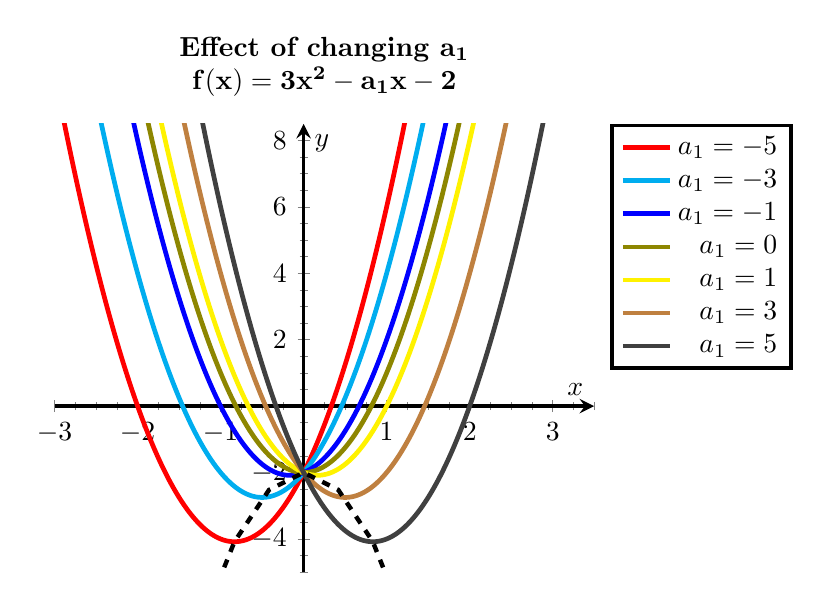
\begin{tikzpicture}
\begin{axis}
[
		minor tick num=3,
		axis x line=middle,
		line width = 1.3,
		align =center,
		title={\textbf{Effect of changing $\bf{a_1}$}\\ $\bf{f(x)=3 x^2 - a_1x -2}$},
		axis y line=middle,
		xmax=3.5, xmin=-3,
		ymax=8.5, ymin=-5,
		xlabel=$x$,ylabel=$y$,
		legend style={
				cells={anchor=east},
				legend pos=outer north east
			}
	]
\foreach \num / \col in {-5/red, -3/cyan,  -1/blue, 0/olive, 1/yellow, 3/brown,  5/darkgray}  {
				\edef\temp{\noexpand\addplot[line width=1.7pt, samples=500, domain= -3:3, color= \col]
					{3*x^2 - \num*x -2};}
        \temp
				 \addlegendentryexpanded{$a_1 = \num$};
}
\addplot[dashed, black, ultra thick] {-3*x^2 -2};
\end{axis}
\end{tikzpicture}
\end{center}
\noindent The effect of changing $a_1$ can be summarized as follows:
\begin{itemize}
\item The value of $a_1$ does not have an influence on how narrow the parabola is.
\item As before all parabolas cross the $y$-axis at the value of $a_0$ which is $-2$ in this case.
\item The extremum of the parabola moves itself along a parabola (dashed line) as $a_1$ changes.
\end{itemize}
\noindent Finally, changing $a_0$ gives:
\begin{center}
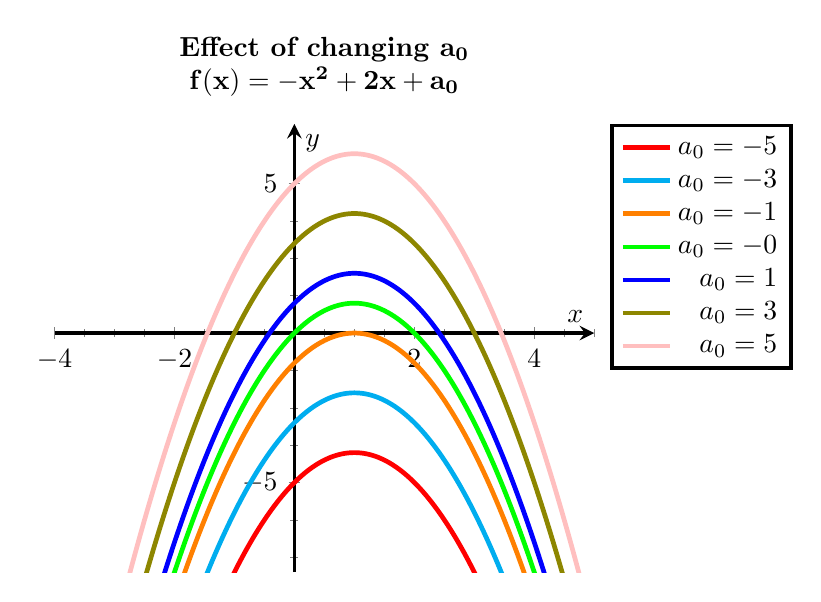
\begin{tikzpicture}
\begin{axis}
[
		minor tick num=3,
		axis x line=middle,
		line width = 1.3,
		align =center,
		title={\textbf{Effect of changing $\bf{a_0}$}\\ $\bf{f(x)=-x^2 + 2x +a_0}$},
		axis y line=middle,
		xmax=5, xmin=-4,
		ymax=7, ymin=-8,
		xlabel=$x$,ylabel=$y$,
		legend style={
				cells={anchor=east},
				legend pos=outer north east
			}
	]
\foreach \num / \col in {-5/red, -3/cyan, -1/orange, -0/green, 1/blue, 3/olive, 5/pink}  {
				\edef\temp{\noexpand\addplot[line width=1.7pt, samples=500, domain= -4:5, color= \col]
					{-x^2 + 2*x +\num};}
        \temp
				 \addlegendentryexpanded{$a_0 = \num$};
}
\end{axis}
\end{tikzpicture}
\end{center}
\noindent Once again the value of $a_0$ is where the parabola crosses the $y$-axis. Changing $a_0$ shifts the parabola vertically without changing it otherwise.

\subsubsection{Solving $2^{nd}$ degree polynomial equations}

\noindent A $2^{nd}$ degree polynomial equation (also known as a quadratic equation) is of the form\footnote{This is usually written as $f(x) = ax^2 + bx + c = 0$ with $a$, $b$ and $c$ real numbers.}:
\begin{equation}
\label{QuadrEq1}
a_2 x^2 + a_1 x + a_0 = 0
\end{equation}
\noindent Solutions are the values of $x$ where the graph of the parabola coincides with the $x$-axis. Looking at figure above we see there can be three different cases:
\begin{enumerate}
\item The red and light blue parabolas do not touch the $x$-axis: there are \textbf{no solutions}.
\item The orange parabola touches the $x$-axis but does not cross it. There is \textbf{exactly one solution}, namely the value of $x$ at that point.
\item The parabola crosses the $x$-axis, in which case there are \textbf{two distinct solutions}.
\end{enumerate}
\noindent In this section we will discuss the solutions in each of the cases. The derivation of these results are given in (\ref{DeriveDiscr}) but can be skipped without running into difficulties in the rest of the text.\\

\noindent In order to calculate the value of the solutions we define $\Delta$\, the \textbf{discriminant}\footnote{The notation "`:="' means "`is defined as"'.}
$$
\Delta := a_1^2 - 4 a_2 a_0
$$ 
The three cases are then the following:
\begin{enumerate}
\item $\mathbf{\Delta > 0:}$\\
\noindent The equation has $2$ distinct solutions:
$$
x_{\pm} = \frac{- a_1 \pm \sqrt{\Delta}}{2 a_2}
$$
\noindent For example in equation $2x^2 -10 x +8 = 0$ the values of the $a_i$'s are
\begin{eqnarray*}
a_2 = 2 & a_1 = -10 & a_0 = 8
\end{eqnarray*}
The discriminant is equal to
$$
\Delta = a_1^2 - 4 a_2 a_0 = (-10)^2 - 4\times 2 \times 8 = 100 - 64 = 36
$$
The $2$ solutions are
\begin{eqnarray*}
x_+ = \frac{-a_1 + \sqrt{\Delta}}{2 a_2} = \frac{-(-10) + \sqrt{36}}{2 \times 2} =  \frac{10 + 6}{4} = 4 \\
x_- = \frac{-a_1 - \sqrt{\Delta}}{2 a_2} = \frac{-(-10) - \sqrt{36}}{2 \times 2} =  = \frac{10 - 6}{4} = 1 
\end{eqnarray*}
\noindent In the graph below we indeed see that the function crosses the $x$-axis twice: at $x=1$ and at $x=4$.
\begin{center}
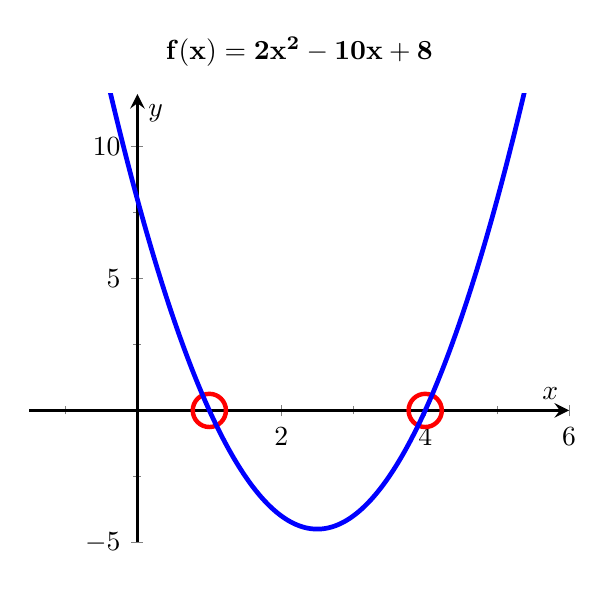
\begin{tikzpicture}
\begin{axis}
[
		minor tick num=1,
		axis x line=middle,
		line width = 1.3,
		title={$\bf{f(x)=2x^2 -10x +8}$},
		axis y line=middle,
		xmax=6, xmin=-1.5,
		ymax=12, ymin=-5,
		xlabel=$x$,ylabel=$y$,
	]
	\draw [red, ultra thick] (1,0) circle [radius=6pt];
\draw [red, ultra thick] (4,0) circle [radius=6pt];
	\addplot[line width=1.7pt, samples=500, domain= -1.5:6, color= blue]
					{2*x^2 -10*x +8};
\end{axis}
\end{tikzpicture}
\end{center}
\item $\mathbf{\Delta = 0:}$\\
\noindent The equation has $1$ unique solution:
$$
x =\frac{- a_1 \pm \sqrt{\Delta}}{2 a_2}=  \frac{-a_1}{2a_2}
$$

In $f(x)=-\frac{1}{2}x^2 -3 x - \frac{9}{2} = 0$ the $a_i$'s are
\begin{eqnarray*}
a_2 = -\frac{1}{2} & a_1 = -3 & a_0 = -\frac{9}{2}
\end{eqnarray*}
The discriminant is equal to
$$
\Delta = a_1^2 - 4 a_2 a_0 = (-3)^2 - 4\times (-\frac{1}{2}) \times (-\frac{9}{2}) = 9 - 9 = 0
$$
The solution is
\begin{equation*}
x = \frac{-a_1 }{2 a_2} = \frac{-(-3)}{2 \times (-\frac{1}{2})} = -3 
\end{equation*}
\begin{center}
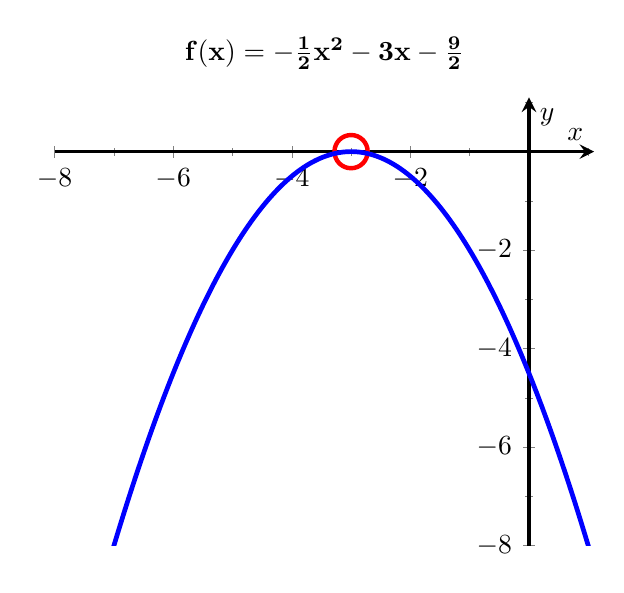
\begin{tikzpicture}
\begin{axis}
[
		minor tick num=1,
		axis x line=middle,
		line width = 1.3,
		title={$\bf{f(x)=-\frac{1}{2}x^2 -3x -\frac{9}{2}}$},
		axis y line=middle,
		xmax=1.1, xmin=-8,
		ymax=1.1, ymin=-8,
		xlabel=$x$,ylabel=$y$,
	]
	\draw [red, ultra thick] (-3,0) circle [radius=6pt];
%\draw [red, ultra thick] (4,0) circle [radius=6pt];
	\addplot[line width=1.7pt, samples=500, domain= -8:1.1, color= blue]
					{-0.5*x^2 -3*x - 4.5};
\end{axis}
\end{tikzpicture}
\end{center}

\item $\mathbf{\Delta < 0:}$\\
\noindent No (real) solutions exist. As an example we consider $f(x)= -x^2 + x-1=0$. The coefficients are
\begin{eqnarray*}
a_2 = -1 & a_1 = 1 & a_0 = -1
\end{eqnarray*}
The discriminant is equal to
$$
\Delta = a_1^2 - 4 a_2 a_0 = 1^2 - 4\times (-1) \times (-1) = -3 < 0
$$
If we were to try to apply the formula $x_{\pm} = \frac{-a_1 \pm \sqrt{\Delta}}{2a_2}$ we would be taking the square root of a negative number, which does not exist. In the corresponding graph we indeed see that the parabola does not touch the $x$-axis anywhere.
\begin{center}
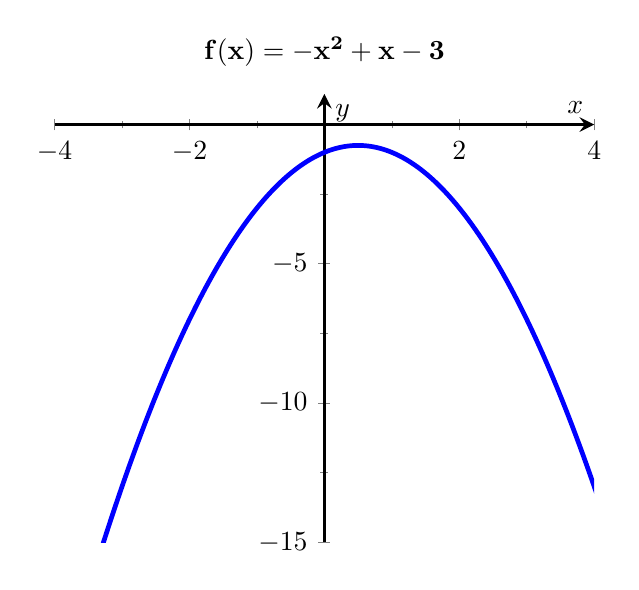
\begin{tikzpicture}
\begin{axis}
[
		minor tick num=1,
		axis x line=middle,
		line width = 1.3,
		title={$\bf{f(x)=-x^2 +x -3}$},
		axis y line=middle,
		xmax=4, xmin=-4,
		ymax=1.1, ymin=-15,
		xlabel=$x$,ylabel=$y$,
	]
	\addplot[line width=1.7pt, samples=500, domain= -4:15, color= blue]
					{-x^2 +x - 1};
\end{axis}
\end{tikzpicture}
\end{center}

\end{enumerate}

\subsection{Higher-order polynomial equations}

\noindent Equations of the form
$$
\sum\limits_{i=1}^{n} a_i x^i = 0
$$
with $n>2$ are not as straightforward to solve. For $n=3$ and $n=4$ there exist techniques to solve such equations, but they are beyond the scope of this text. From $n=5$ onwards there exists no general technique to solve the polynomial equation and we are left with approximation techniques for estimating the solutions\footnote{When I say there are no techniques I do not mean that we have not found a technique yet but we keep on looking for one. It is actually much cooler. Mathematicians have been able to prove that no technique could ever be developed or found to do this because there simply is none. Told you, it's cool!}. These will be discussed when we come across them in physical applications. Just to get the flavor, here is what a randomly chosen $7^{th}$ degree polynomial looks like.
\begin{center}
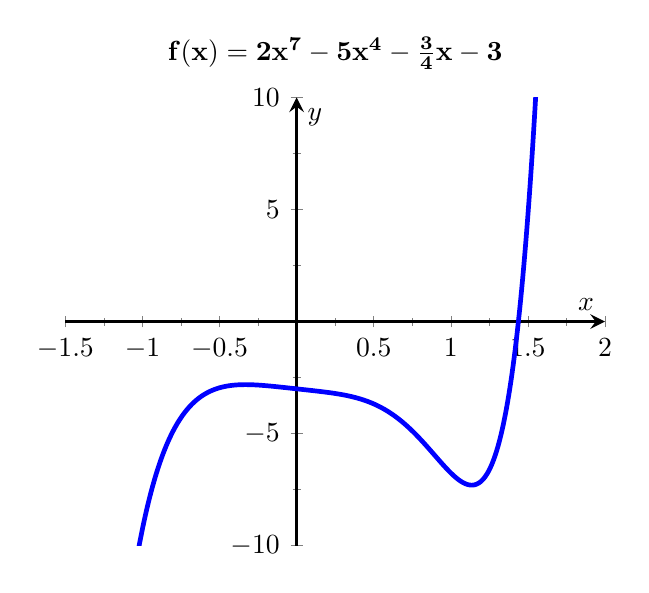
\begin{tikzpicture}
\begin{axis}
[
		minor tick num=1,
		axis x line=middle,
		line width = 1.3,
		title={$\bf{f(x)=2x^7 -5x^4 -\frac{3}{4}x -3}$},
		axis y line=middle,
		xmax=2, xmin=-1.5,
		ymax=10, ymin=-10,
		xlabel=$x$,ylabel=$y$,
	]
	\addplot[line width=1.7pt, samples=500, domain= -1.5:2, color= blue]
					{2*x^7 - 5*x^4 - 0.75*x - 3};
\end{axis}
\end{tikzpicture}
\end{center}

\section{Functions in physics}

\noindent Functions are among the most frequently used mathematical concepts in the sciences. They are the physicist's way of representing dependencies between physical quantities.\\

\begin{itemize}

\item \textbf{Scattering: }\\
\noindent Imagine we have an object of unknown shape which we wish to determine. We decide to shoot some tiny balls (or light or electrons or yodeling lemmings of known shape) at the object at different incoming angles and measure for each the corresponding outgoing angle.
\begin{center}
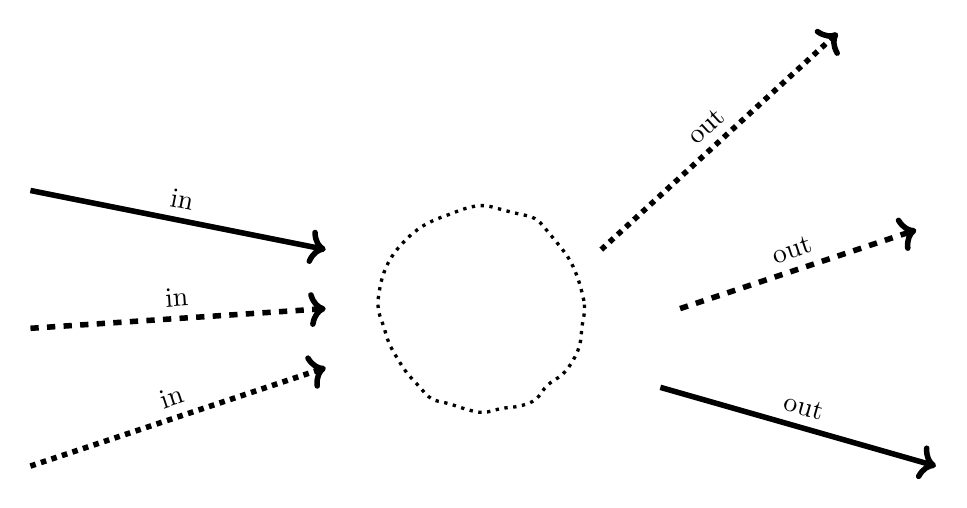
\begin{tikzpicture} [scale = 0.5]
\coordinate (c) at (6,1);
\draw[dotted, black, rounded corners=1mm, very thick] (c) \irregularcircle{2.6cm}{1mm};
	\draw[->] [line width=2pt, solid] {(-5.5,4) -- node[sloped, anchor=center, above]{in} (2,2.5)};
	\draw[->] [line width=2pt, dashed] {(-5.5,0.5) -- node[sloped, anchor=center, above]{in}(2,1)};
	\draw[->] [line width=2pt, dotted] {(-5.5,-3) -- node[sloped, anchor=center, above]{in}(2,-0.5)};
	
	\draw[->] [line width=2pt, dotted] {(9,2.5) -- node[sloped, anchor=center, above]{out} (15,8)};
	\draw[->] [line width=2pt, dashed] {(11,1) -- node[sloped, anchor=center, above]{out}(17,3)};
	\draw[->] [line width=2pt, solid] {(10.5,-1) -- node[sloped, anchor=center, above]{out}(17.5,-3)};
	
\end{tikzpicture}	
\end{center}
\noindent The outgoing angle can is a function of the incoming angle: $\alpha_{out} = f(\alpha_{in})$.

\item \textbf{Parabolic motion: }\\
\noindent Take an apple in your hand and throw it out in front of you. The motion of the apple once it leaves your hand looks something like this:\\
\begin{center}
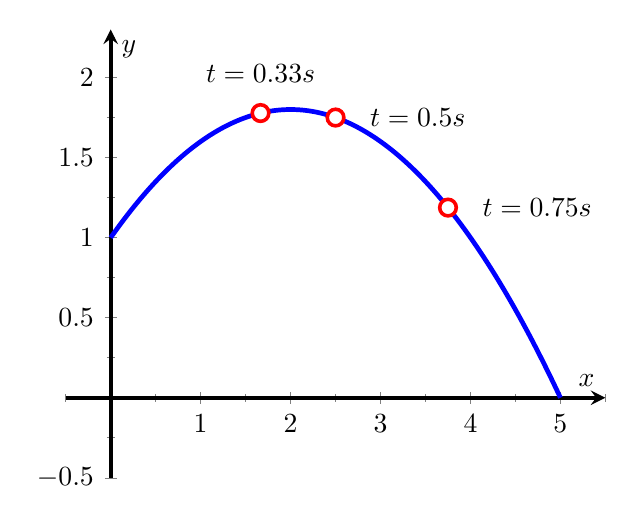
\begin{tikzpicture}
\begin{axis}
[
		minor tick num=1,
		axis x line=middle,
		line width = 1.3,
		%title={$\bf{f(x)=2x^7 -5x^4 -\frac{3}{4}x -3}$},
		axis y line=middle,
		xmax=5.5, xmin=-0.5,
		ymax=2.3, ymin=-0.5,
		xlabel=$x$,ylabel=$y$,
	]
	\addplot[line width=1.7pt, samples=500, domain= 0:5, color= blue]
					{-0.2*(x+1)*(x-5)};
	\draw [red, fill=white,] (1.666,1.778) circle [radius = 3pt] node [above=2.5mm , black]{$t = 0.33 s$};
	\draw [red, fill=white,] (2.5,1.75) circle [radius = 3pt] node [right=3mm,black]{$t = 0.5 s$};
	\draw [red, fill=white,] (3.75,1.1875) circle [radius = 3pt]node [right=3mm,black]{$t = 0.75 s$};
	
\end{axis}
\end{tikzpicture}
\end{center}
What is shown is actually a parametric representation of the trajectory of the apple. Both the horizontal ($x$) and the vertical ($y$) position of the apple are functions of the parameter $t$ which represents the time since the apple left your hand: $\left( x(t), y(t) \right)$. We choose to call that moment time $t=0$. The apple is then where your hand left it:$\left( x(0), y(0) \right) = (0,1)$. It moves upwards until its highest point where it starts making its way to the ground, all the while moving further away from you. The position of the apple after $1/3 s$, $1/2 s$ and $3/4 s$ is marked on the graph.
\item \textbf{Distance as a function of time: }
\begin{equation}
\label{Flight_equation}
d(t) = 5\:500\:000 - 280 t
\end{equation}
\noindent I just made up this equation on the spot. It could for instance describe the distance you still have to travel when flying from London to New York. We start our chronometer at the moment of take-off, which we call time $t=0$. At that instant of time you are in London which is approximately $5\:500$ km from New York. Plugging $t=0$ into equation (\ref{Flight_equation}) we find that the distance to our destination at that time equals $d(0) = 5\:500\:000 - 280 \times 0 = 5\:500\:000 $. This is the number of meters that we still have to travel at time $t=0$. After 3 hours of flight the remaining distance to New York is $d(10\:800) = 5\:500\:000 - 280 \times 10\:800 = 2\:476\:000 $ meters, or $2 \:476$ km to New York. Notice that we express the time in second and that an hour corresponds to $3\:600$ seconds so that 3 hours correspond to $10\:800$ seconds.
\item \textbf{Pressure as a function of depth: }
\begin{equation}
\label{Press_Examp}
p(d) = 1 + \frac{d}{10}
\end{equation}
\noindent In our everyday life we experience the "`normal"' pressure due to the atmosphere (aptly called "`atmospheric pressure"'). In a swimming pool the pressure increases as we dive deeper under water. The pressure $p$ we experience under water is thus a function of the depth $d$ at which we find ourselves. Equation (\ref{Press_Examp}) gives the amount of pressure we experience at a depth $d$ under water. At the surface the depth $d=0$ and we experience (one) atmospheric pressure. Diving to a depth of 5 meters we experience a pressure equal to $p(5) = 1+ \frac{5}{10} = 1 + 0,5 = 1,5 $ atmospheric pressure. It has increased by 50\%. At 30 meters depth we experience $p(30) = 1 + \frac{30}{10} = 1 + 3 = 4$ times the atmospheric pressure.
\item \textbf{Radiated power as a function of temperature: }
\begin{equation}
 P(T) = T^4
\label{StefBoltz}
\end{equation}
\noindent Objects radiate more when they are hotter. The hotter a piece of coal is, the more heat it radiates per second. The amount of energy radiated per second is known as the power $P$. This power is a function of temperature\footnote{The temperature $T$ in equation (\ref{StefBoltz}) needs to be expressed in a unit known as Kelvin instead of degrees centigrade. We will discuss the Kelvin temperature scale in chapter \ref{}. For now just remember that the equation only gives correct results if $T$ is expressed in Kelvin.}: $P(T)$. The $4^{th}$ power in the function says that if the temperature doubles, the power becomes $16$ times larger (because $2^4 = 16$). Or equally that if the temperature is tripled, the power increases $81$ times (because $3^4 = 81$).
\end{itemize}
\noindent One of the objectives of science is to find such relations between physical quantities. Writing down a function that relates several quantities amounts to making a prediction about reality. Equation (\ref{Press_Examp}) predicts that at a depth of 10 meters under the water surface the pressure will be twice its value at the surface. This can be tested. And if this turns out to be wrong (it does not) than a new relation between pressure and depth needs to be looked for.

\section{Proof that $\sqrt{2}$ is irrational}
\label{proofsqrt2}
\noindent We want to prove that $\sqrt{2}$ cannot be written as a fraction of integers. One possible way of doing this is to assume it can, and show that this assumption leads to an impossible conclusion (which mathematicians call a contradiction).\\

\noindent Before proving it, we prove a simple property of even numbers which we will need below: $ x^2 \text{even} \Rightarrow x \text{even} $, if a number $x^2$ is even, than so is $x$ itself. How do we know this? Well, if $x$ was odd, than it could be written as $x= 2n + 1$ for $n \in \mathbb{N}$ (any even number is twice some natural number and any odd number is an even number plus $1$). Its square can be calculated with the formula $\left( a+b  \right)^2 = a^2 + 2ab+b^2$. So
$$
x^2 = \left( 2n + 1 \right)^2 = 4n^2 + 4n + 1
$$
Both $4n^2$ and $4n$ are even (as they are both $2$ times some natural number) which because of the $+1$ at the end shows that $x^2$ is odd. This proves $x^2 \text{even} \Rightarrow x \text{even}$, because we just saw that if $x$ had been odd, so would have been its square.\\

\noindent We now start the actual proof of the irrationality of $\sqrt{2}$ by assuming
$$
\sqrt{2} = \frac{a}{b}
$$
with $a$ and $b$ integers. Remember than any rational number can be represented by infinitely many fractions. For example
$$
\frac{66}{12} = \frac{22}{4} = \frac{55}{10} = \frac{11}{2} = \cdots
$$
\noindent are all equivalent and $\frac{11}{2}$ is the most simplified this fraction can be. We may as well choose $a$ and $b$ so that $\frac{a}{b}$ is as simplified as possible. Otherwise, we could simplify it until it cannot be simplified any further and call the numerator and denominator of that fraction $a$ and $b$, respectively. So we now know that $\sqrt{2} = \frac{a}{b}$, that $a$ and $b$ are integers and that the fraction cannot be simplified further. Let us square that equation, which gives
$$
2 = \frac{a^2}{b^2}
$$
\noindent Multiplying both sides by $b^2$ we find
$$
2 b^2 = a^2
$$
\noindent Because $a^2$ is equal to twice some number, it has to be even and by the property we proved above it follows that $a$ itself is even. It can therefore be written as $a=2c$ with $c \in \mathbb{N}$. Pluggin it into the previous equation gives
$$
2 b^2 = \left( 2 c \right)^2 = 4 c^2
$$
\noindent Dividing by $2$ leaves us with
$$
b^2 = 2c^2
$$
\noindent This now proves that $b$ is also even, which at its turn shows that $b$ itself is even. We conclude that both $a$ and $b$ are even. But this is in contradiction with the assumption that $\frac{a}{b}$ cannot be simplified further, as the fraction could be divided by $2$ if they are both even. The only assumption we made is that $\sqrt{2}$ could be written as $\frac{a}{b}$ with $a$ and $b$ integers and it lead us to a contradiction. Therefore the assumption itself cannot be true and $\sqrt{2}$ cannot be written as a fraction of integers.

\section{Derivation of solutions for quadratic equations}
\label{DeriveDiscr}

\noindent The objective is to find the solution(s) of
\begin{equation*}
a_2 x^2 + a_1 x + a_0 = 0
\end{equation*}
if they exist. We start by dividing the equation by $a_2$ which gives
\begin{equation*}
x^2 + \frac{a_1}{a_2} x + \frac{a_0}{a_2} = 0
\end{equation*}
We now add and subtract $\frac{a_1^2}{4 a_2^2}$ from the LHS. Of course adding and subtracting the same number does not alter anything.
\begin{equation*}
x^2 + \frac{a_1}{a_2} x + \frac{a_1^2}{4 a_2^2} - \frac{a_1^2}{4 a_2^2} + \frac{a_0}{a_2} = 0
\end{equation*}
The two last terms are subtracted from the both sides which yields
\begin{equation*}
x^2 + \frac{a_1}{a_2} x + \frac{a_1^2}{4 a_2^2} = \frac{a_1^2}{4 a_2^2} - \frac{a_0}{a_2}
\end{equation*}
This can be rewritten as
\begin{equation*}
\left( x + \frac{a_1}{2a_2} \right)^2 = \frac{1}{4a_2^2} \left( a_1^2 - 4 a_2 a_0 \right)
\end{equation*}
\noindent To convince yourself of this, try working out these expressions. For the LHS use the formula $(a+b)^2 = a^2 + 2ab + b^2$, with in this case $a=x$ and $b = \frac{a_1}{2a_2}$. For the RHS use distributivity: $a (b+c) = ab + ac$. Once you are convinced that it is correct, take the square root of both sides (and remember that taking the square root has 2 solutions) which gives
\begin{equation*}
x + \frac{a_1}{2a_2}  = \pm \frac{1}{2a_2} \sqrt{ a_1^2 - 4 a_2 a_0 }
\end{equation*}
Isolating $x$ on the LHS leaves us with
\begin{equation*}
x =   \frac{-a_1  \pm \sqrt{ a_1^2 - 4 a_2 a_0 }}{2a_2}
\end{equation*}
Defining the discriminant as $\Delta = a_1^2 - 4 a_2 a_0$ we finally find
\begin{equation*}
x =   \frac{-a_1  \pm \sqrt{ \Delta }}{2a_2}
\end{equation*}
In the step in which the square root of the equation was taken, it was assumed that we were allowed to do so. But remember that the square root of negative numbers does not exist (in the reals). In other words we are not allowed to take the square root and therefore no solutions exist if $\Delta < 0$. If $\Delta = 0$ than both solutions give the same result, namely $x = \frac{-a_1}{2 a_2}$. And if $\Delta > 0$ then both solutions are distinct and given by $x_{\pm} = \frac{-a_1 \pm \sqrt{\Delta}}{2a_2}$.

%\subsection{Functions of several variables}

%\subsubsection{Composition of functions}
\chapter{Getting back in shape}

\epigraph{Puisque tu fais de la géométrie et de la trigonométrie, je vais te donner un problème: Un navire est en mer, il est parti de Boston chargé de coton, il jauge $200$ tonneaux. Il fait voile vers le Havre, le grand mât est cassé, il y a un mousse sur le gaillard d’avant, les passagers sont au nombre de douze, le vent souffle N.-E.-E., l’horloge marque $3$ heures un quart d’après-midi, on est au mois de mai…. On demande l’âge du capitaine.}{\textit{Lettre à Caroline, $16$ May $1841$ \\ Gustave Flaubert}}

\noindent The mathematics necessary to do physics covers quite a wide range of topics. Though few are as important as the study of basic geometric shapes, angles and trigonometric functions. The goal of this chapter is to introduce enough of each of these topics with the physics that is to come in mind. We will focus on $2$-dimensional shapes for now\footnote{The concept of dimension will be formally introduced in chapter \ref{Coordinates}.}.\\

\noindent We start by introducing a couple of basic geometric concepts.
\begin{itemize}
\item \textbf{Arc length: }length of (part of) a curve when followed from some initial point to a final point (e.g. the distance you would have traveled after walking along the grey part of the curve below from point $A$ to point $B$). 
\item \textbf{Perimeter: }length of the outer boundary of a closed $2$-dimensional shape. Or equally, the arc length of $1$ full loop around the shape.
\item \textbf{Circumference: }perimeter of a circle or ellipse.
\item \textbf{Area: }"amount" of space enclosed by a $2$-dimensional closed shape.
\end{itemize}
Each of these is represented in grey below:
\begin{center}
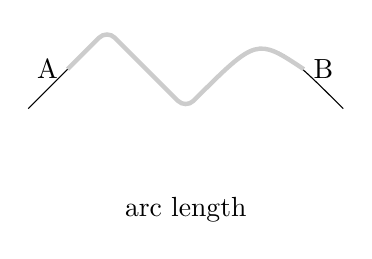
\begin{tikzpicture}
\title{Arc length}
 \draw [rounded corners] (0,0) -- (1,1) 
           -- (2,0) .. controls (3,1) .. (4,0); 
	\draw [rounded corners,gray!40!white, ultra thick] (0.5, 0.5) -- (1,1) 
           -- (2,0)..controls (2.9,0.9)..(3.5,0.5);
	\node [below=1cm, align=flush center] at (2,0){arc length};
\node[left] at (0.5, 0.5){A};
\node[right] at (3.5, 0.5){B};
\end{tikzpicture}
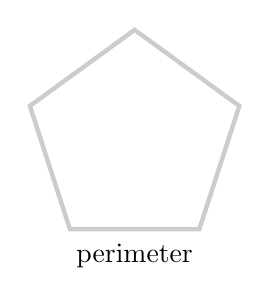
\begin{tikzpicture}
	\node[regular polygon, regular polygon sides=5, draw, inner sep=0.8cm, color = gray!40!white, ultra thick] at (0,0) {};
	\node [below=1.2cm, align=flush center] at (0,0){perimeter};
\end{tikzpicture}

\begin{tikzpicture}
\draw [gray!40!white, ultra thick] (0,0)circle [radius = 1cm];
\node [below=1cm, align=flush center] at (0,0){circumference};
\end{tikzpicture}
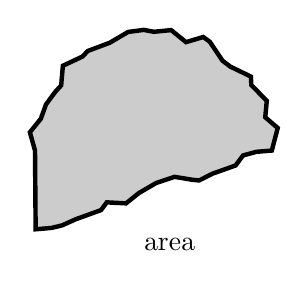
\begin{tikzpicture}
\draw [fill=gray!40!white,xshift=2cm, ultra thick,
decoration={random steps,segment length=2mm}]
decorate { (0,0) -- (3,1) arc (0:180:1.5)} -- cycle;
\node [below=1cm, align=flush center] at (3.7,1){area};
\end{tikzpicture}
\end{center}

\section{The circle}

\noindent Choose a point somewhere in the middle of a sheet of paper. We will call this point $m$ and refer to it as the "center" of the circle.  Draw a dot exactly 2 cm away from $m$. Draw another point also 2 cm away from $m$. And another. And another,... . If you draw all points that are a distance of 2 cm away from M you will have drawn something that looks like this:
\begin{center}
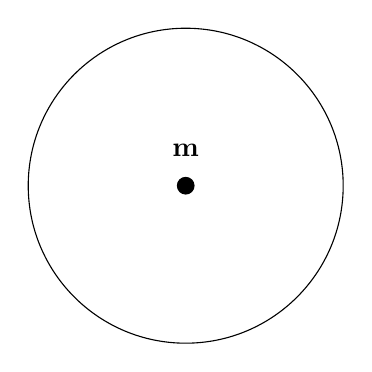
\begin{tikzpicture}
\draw (0,0)circle [radius = 2cm];
\filldraw (0,0) circle [radius = 3pt] node[above=2.5mm]{\textbf{m}};
\end{tikzpicture}
\end{center}
\noindent This is a \textbf{circle} of radius $2$ cm and center $m$. The \textbf{radius} of a circle is the distance from its center to any of its points. The \textbf{diameter} is the distance from any point of the circle to a point exactly opposite it. The line connecting such $2$ points passes through the center and has length $d = 2R$.
\begin{center}
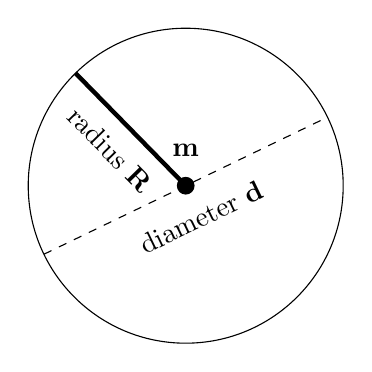
\begin{tikzpicture}
\draw (0,0) circle [radius = 2cm];
\filldraw (0,0) circle [radius = 3pt] node[above=2.5mm]{\textbf{m}};
\draw [ultra thick] (0,0) -- node[sloped, anchor=center,below=1mm]{radius $\bf{R}$}(-1.4,1.43);
\draw [dashed] (-1.8,-0.87) -- node[sloped, anchor=center,below=2mm]{diameter $\bf{d}$}(1.8,0.87);
\end{tikzpicture}
\end{center}
\noindent Though the circle is a seemingly simple geometric figure, it has several interesting and some non-intuitive properties. All circles, no matter how large or small, share the following property: \textbf{The circumference of the circle divided by its diameter is equal to $\pi$}. This is actually one of the multiple ways to define $\pi$:
\begin{equation}
\label{DefPi}
\frac{\textit{circumference of circle}}{\textit{diameter}} = \frac{\textit{circumference of circle}}{2 R} = \pi
\end{equation}
\noindent The number $\pi$ is often approximated by $3.14$, but as was mentioned in section \ref{RealNumbersSet}, $\pi$ is actually an irrational number and as such has an infinite non-repeating decimal tail. Multiplying both sides of equation (\ref{DefPi}) by $2R$ gives us the formula for the circumference $C$ of a circle:
\begin{equation}
\label{CircumCirc}
C = 2 \pi R
\end{equation}
A circle with radius $R$ can be shown to have area $A$ equal to\footnote{In chapter \ref{IntegralChapter} we will discuss techniques to prove this and similar formulas.}
\begin{equation}
A = \pi R^2
\end{equation}
\noindent One consequence of this is that if we draw a second circle with radius twice as large as the first one, its circumference will also be doubled but the area will be $4$ times larger (because of square in the formula for the area).

\section{Looking at it from a different angle}

\noindent Let us look at two (straight) lines $L_1$ and $L_2$. There are 3 possible cases:
\begin{center}
\begin{tikzpicture}
\draw (-2,-2) node [right=0.2cm]{$L_1$}-- (2,2);
\draw (-2,-2) node [left= 0.2cm]{$L_2$}-- (2,2);
%\draw (-3,0) node[above] {$L_2$} -- (2,1);
\end{tikzpicture}
\begin{tikzpicture}
\draw (-2,-2) node [below]{$L_1$}-- (2,2);
\draw (-3,0) node[above] {$L_2$} -- (2,1);
\end{tikzpicture}
\begin{tikzpicture}
\draw (-2,-2) node [right=0.2cm]{$L_1$}-- (2,2);
\draw (-2,-1) node[left=0.2cm] {$L_2$} -- (2,3);
\end{tikzpicture}
\end{center}
\begin{enumerate}
\item \textbf{Equal lines} are completely overlapping and thus have infinitely many points in common.
\item \textbf{Intersecting lines} have exactly $1$ point in common.
\item \textbf{Parallel lines} never touch and thus have no points in common. This is written as $L_1 \parallel L_2$.
\end{enumerate}
\noindent Whenever $2$ lines intersect, they form $4$ "openings" between them, known as \textbf{angles}.
\begin{center}
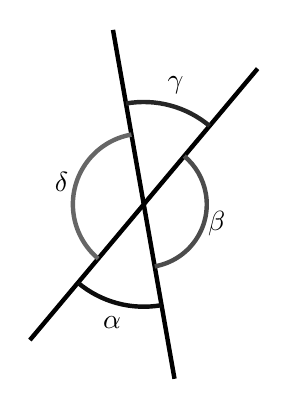
\begin{tikzpicture}[scale = 1.5]
\coordinate (A) at (-130:1.5);
\coordinate (B) at (0,0);
\coordinate (C) at (50:1.5);
\coordinate (D) at (-80:1.5);
\coordinate (E) at (100:1.5);
\draw [ultra thick] (A) -- (C);
\draw [ultra thick] (D) -- (E);
\draw[color=black, ultra thick] pic["$\alpha$", draw=gray!10!black, ultra thick, angle eccentricity=1.2, angle radius=1.3cm] {angle=A--B--D};
\draw pic["$\beta$", draw=gray!60!black, ultra thick, angle eccentricity=1.2, angle radius=0.8cm] {angle=D--B--C};
\draw pic["$\gamma$", draw=gray!30!black, ultra thick, angle eccentricity=1.2, angle radius=1.3cm] {angle=C--B--E};
\draw pic["$\delta$", draw=gray!80!black, ultra thick, angle eccentricity=1.2, angle radius=0.9cm] {angle=E--B--A};
\end{tikzpicture}
\end{center}
\noindent In \ref{Degr} and \ref{Radi} we will introduce two different units for angles. Afterwards, in \ref{AngRel} we will discuss some relations between angles, and we will show for example that it is sufficient to know $1$ one of the angles above, to know all of them.

\subsection{degrees}
\label{Degr}

\noindent For now, we focus on any of the angles formed by the $2$ lines and disregard the others. We take a horizontal line and consider the angle formed by rotating a second line around it. 
\begin{center}
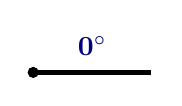
\begin{tikzpicture}[scale = 1.5]
\coordinate (A) at (1,0);
\coordinate (B) at (0,0);
\coordinate (C) at (0:1cm);
\filldraw[fill=blue!20!white, draw=blue!50!black] (0,0) -- (7mm,0mm)
	arc [start angle=0, end angle=0, radius=7mm, color=black] -- cycle;
\draw (A) -- (B) -- (C)[color=black, ultra thick];
\node [node font=\normalsize, color=blue!50!black] at (0.5,0.22) {$\bf{0^{\circ}}$};
\filldraw (B) circle [radius=1.2pt];
\end{tikzpicture}
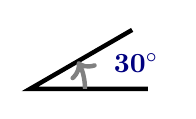
\begin{tikzpicture}[scale = 1.5]
\coordinate (A) at (1,0);
\coordinate (B) at (0,0);
\coordinate (C) at (30:1cm);
\draw (A) -- (B) -- (C)[color=black, ultra thick] pic[draw=gray, ultra thick, ->, angle eccentricity=1.2, angle radius=7mm]
    {angle=A--B--C};
\node [node font=\normalsize, color=blue!50!black] at (0.9,0.22) {$\bf{30^{\circ}}$};
\end{tikzpicture}
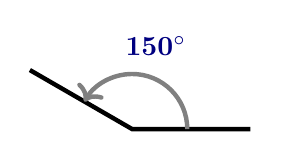
\begin{tikzpicture}[scale = 1.5]
\coordinate (A) at (1,0);
\coordinate (B) at (0,0);
\coordinate (C) at (150:1cm);
\draw (A) -- (B) -- (C)[color=black, ultra thick]
	pic[draw=gray, ultra thick, ->, angle eccentricity=1.2, angle radius=7mm]
    {angle=A--B--C};
\node [node font=\normalsize, color=blue!50!black] at (0.2,0.7) {$\bf{150^{\circ}}$};
\end{tikzpicture}
\begin{tikzpicture}[scale = 1.5]
\coordinate (A) at (1,0);
\coordinate (B) at (0,0);
\coordinate (C) at (220:1cm);
\draw (A) -- (B) -- (C)[color=black, ultra thick]pic[draw=gray, ultra thick, ->, angle eccentricity=1.2, angle radius=7mm]
    {angle=A--B--C};
\node [node font=\normalsize, color=blue!50!black] at (0,0.7) {$\bf{220^{\circ}}$};
\end{tikzpicture}
\begin{tikzpicture}[scale = 1.5]
\coordinate (A) at (1,0);
\coordinate (B) at (0,0);
\coordinate (C) at (300:1cm);
\draw (A) -- (B) -- (C)[color=black, ultra thick]
	pic[draw=gray, ultra thick, ->, angle eccentricity=1.2, angle radius=7mm]
    {angle=A--B--C};
\node [node font=\normalsize, color=blue!50!black] at (0,0.7) {$\bf{300^{\circ}}$};
\end{tikzpicture}
\begin{tikzpicture}[scale = 1.5]
\coordinate (A) at (1,0);
\coordinate (B) at (0,0);
\coordinate (C) at (359.9:1cm);
\draw (A) -- (B) -- (C)[color=black, ultra thick]
	pic[draw=gray, ultra thick, ->, angle eccentricity=1.2, angle radius=7mm]
    {angle=A--B--C};
\node [node font=\normalsize, color=blue!50!black] at (0,0.9) {$\bf{360^{\circ}}$};
\end{tikzpicture}
\end{center}
\noindent One common unit for angles is known as \textbf{degrees} denoted by the symbol $\bf{^\circ}$. When the lines are overlapping (or simply parallel) the angle is said to be a $0^{\circ}$ angle. A full rotation\footnote{The historical reason for dividing the circle into $360^{\circ}$ is not exactly known. One often-stated hypothesis is that this is part of the legacy of the Babylonian sexagecimal numeral system (base 60) that also gave us the division of an hour into 60 minutes and a minute into 60 seconds.} corresponds to $360^{\circ}$. Therefore an angle of $0^{\circ}$ and one of $360^{\circ}$ are equal.\\

\noindent We emphasize that there is no logical reason why a circle has to be divided into exactly $360$ equal parts. Below is a circle divided into $10$ equal parts. We could have called the angle of each of these parts a zorm and circles would therefore be constituted of $10$ zorms. For historical reasons though the convention is to divide circles into $360$ equal slices where the angle of one such slice is called one degree.

\begin{center}
\begin{tikzpicture}
\draw (0,0) circle [radius = 2];
\foreach \ang in {0,36,...,360}{
	\draw [color=blue!50!black ,ultra thin] (0,0) -- (\ang:2);
	}
\end{tikzpicture}
\begin{tikzpicture}[scale=1.3]
\draw [ultra thick] (0,0) -- (60:1.9);
\draw [ultra thick] (0,0) -- (290:1.9);
\coordinate (A) at (0:2);
\coordinate (B) at (0,0);
\coordinate (C) at (60:1.3cm);
\coordinate (D) at (290:1cm);
\coordinate (E) at (-70:0.7cm);
\draw [ultra thick] (0,0) -- (2.2,0);
\draw pic["$\bf{60^{\circ}}$",draw=black, ultra thick, ->, angle eccentricity=1.5, angle radius=1.5cm] {angle=A--B--C};
\draw pic["$\bf{290^{\circ}}$",draw=black, ultra thick, ->, angle eccentricity=1.5, angle radius=0.7cm] {angle=A--B--D};
\draw pic["$\bf{-70^{\circ}}$",draw=gray!70!black, ultra thick, <-, angle eccentricity=1.5, angle radius=1cm] {angle=E--B--A};
\end{tikzpicture}
\end{center}
\noindent By convention, angles are positive if they are counterclockwise and negative if they are clockwise (also here, there is no logic to this, it is simply a historical convention). The absolute value of the angle tells us how large the opening between the $2$ lines is. Its sign tells us whether the opening is to be considered clockwise (negative) or counterclockwise (positive). As you can see on the figure the same two lines form both the angle of $290^{\circ}$ and that of $-70^{\circ}$. The difference is only whether we consider the opening to be read clockwise or counterclockwise.\\

\noindent Angles can also have absolute value larger than $360^{\circ}$. For instance, $420^{\circ}$ is a full circle plus an opening of $60^{\circ}$.
\begin{center}
\begin{tikzpicture}
 \draw [ultra thick] ( 0,0) -- (3,0);
 \draw [ultra thick] (0,0) -- (60:3); 
%\draw [dashed, black,->] () arc (); 

\draw [->,very thick, dotted] (1.5,0) arc [start angle=0, end angle=58, radius=1.5];

%(1.5,0) arc[start angle=0, end angle = 60,  radius = 1.5,->] (60:1.5);
\node[black] at (2.2, 0.8) {$60^{\circ}$};
 \bigangle[gray,dashed]{420};
\end{tikzpicture}
\end{center}
\noindent These angles represent the same opening between the two lines. The grey one is just thought of as having made a full circle prior to ending up at the same place as the line of the $60^{\circ}$ angle.\\

\noindent When $2$ lines form an angle of $90^{\circ}$ the angle is called a \textbf{right} angle and the lines are said to be \textbf{perpendicular}, written as $L_1 \perp L_2$. Right angles are marked in figures in the following manner: 
\begin{center}
\begin{tikzpicture}
\coordinate (A) at (3, 0) {};
        \coordinate (B) at (0, 0) {};
        \coordinate (C) at (0, 2) {};
\tkzMarkRightAngle[size=.7](A,B,C);
\tkzLabelAngle[dist=.5](A,B,C){};
 \draw [ultra thick] (B) -- (A);
 \draw [ultra thick] (B) -- (C); 
\end{tikzpicture}
\end{center}

\subsection{Radians}
\label{Radi}

\noindent What is the relation between an angle $\alpha$ and the size of the arc length $L$ formed by it?
\begin{center}
\begin{tikzpicture}[scale= 2.2]
\draw [dashed, gray] (0,0) circle [radius = 1];
\coordinate (A) at (-30:1);
\coordinate (B) at (0,0);
\coordinate (C) at (45:1);
\draw [black!50!brown,thin] (B) -- node[sloped, anchor=center,below=2mm]{$R$}(A);
\draw [black!50!brown, thin] (B) -- (C);
\draw pic["$\bf{\alpha}$",draw=blue!80!black, dashed, angle eccentricity=1.3, angle radius=1.3cm] {angle=A--B--C};
\draw pic["$\bf{L}$",draw=blue!50!black, ultra thick, angle eccentricity=1.2, angle radius=2.2cm] {angle=A--B--C};
\end{tikzpicture}
\end{center}
\noindent Equation (\ref{CircumCirc}) tells us that if $\alpha=360^{\circ}$ then $L=2\pi R$, the circumference of the circle. If we choose angle $\alpha=180^{\circ}$, corresponding to half the angle of a full circle, the arc length $L$ would be half the circumference of the full circle: $L=\frac{2 \pi R}{2} = \pi R$. An angle of $90^{\circ}$, which is a quarter circle, creates an arc length of a quarter of the circumference of the circle: $L = \frac{2 \pi R}{4} = \frac{\pi R}{2}$. This reasoning holds for any angle. For instance, an angle $\alpha = 36^{\circ}$ corresponding to one tenth of a full circle (i.e. $\frac{36}{360} = \frac{1}{10}$) covers an arc length of one tenth of the circumference: $L = \frac{2 \pi R}{10} = \frac{\pi R}{5}$.\\

\noindent As mentioned earlier, the choice of dividing the circle into $360$ equal parts and calling the size of each a degree is an arbitrary choice made by accidents of history. Instead of dividing the circle into $360$ equal parts, we divide it into $2\pi$ parts (which is approximately $2\times 3.14 = 6.28$) and we call each part a \textbf{radian}. A full circle corresponds therefore to an angle of $2 \pi$ radians, half a circle to $\pi$ radians and so forth. The advantage of this unit is that it explicitly relates the size of the angle with the length of the arc length it forms: an angle of size $\alpha$ radians, in a circle of radius $R$ forms an arc length equal to
\begin{equation}
\label{WrongRadians}
L = R \alpha
\end{equation}
\noindent Can we see that easily? Take for instance $\alpha = 2\pi$ (a full circle), than the arc length is according to (\ref{WrongRadians}) equal to $L = R 2 \pi $, which is indeed the circumference of the circle. Or if we take $\alpha=\frac{\pi}{2}$ (a quarter of a circle), the arc length is $L = R \frac{\pi}{2} = \frac{2 \pi R}{4}$ which is indeed the arc length of a quarter of a circle. Keep the following in mind when working with radians:
\begin{enumerate}
\item The unit radian is often abbreviated as rad. But it is actually more common to omit it altogether and speak about an angle of for instance $\frac{\pi}{4}$ instead of $\frac{\pi}{4}$ rad. This is only done with radians, not with degrees.
\item A negative arc length or a negative radius is meaningless. Lengths are always positive. But angles can be negative and so negative radians do make sense. Remember, a negative angle simply means that it is considered clockwise. Equation (\ref{WrongRadians}) is therefore wrong for negative angles. A correcter version is 
\begin{equation}
L = R |\alpha|
\end{equation}
\item Whenever $\alpha$ is larger than $2\pi$, the arc length $L$ is to be understood as the arc length of the angle plus however many times a full circle is covered. For instance, an angle of $5 \pi$ radians corresponds to $2$ full circumferences ($ 2 \times 2 \pi R$) plus half a circumference ($\frac{2 \pi R}{2}$) which gives a total arc length of $ 2 \times 2 \pi R + \frac{2 \pi R}{2} = 4 \pi R + \frac{2 \pi R}{2} = 5 \pi R$. 
\end{enumerate}
\noindent Degrees and radians are simply different units for the same quantity: angles. Below is a table with corresponding values in both units.\\
\begin{center}
\begin{tabular}{ |c|c|c| }
  \hline
  Figure & Degrees & Radians\\
  \hline
	& & \\
  \begin{tikzpicture}[scale = 1.5]
\coordinate (A) at (1,0);
\coordinate (B) at (0,0);
\coordinate (C) at (0:1cm);
\filldraw[fill=blue!20!white, draw=blue!50!black] (0,0) -- (7mm,0mm)
	arc [start angle=0, end angle=0, radius=7mm] -- cycle;
\draw (A) -- (B) -- (C)[color=black, ultra thick];
\filldraw (B) circle [radius=1.2pt];
\end{tikzpicture} & $0$ & $0$\\& & \\
\hline
& & \\
	\begin{tikzpicture}[scale = 1.5]
\coordinate (A) at (1,0);
\coordinate (B) at (0,0);
\coordinate (C) at (30:1cm);
\draw (A) -- (B) -- (C)[color=black, ultra thick] pic[draw=gray!50!white, ultra thick, ->, angle eccentricity=1.2, angle radius=7mm]
    {angle=A--B--C};
\end{tikzpicture} & $30$ & $ \pi / 6$\\& & \\
	\hline
	& & \\
		\begin{tikzpicture}[scale = 1.5]
\coordinate (A) at (1,0);
\coordinate (B) at (0,0);
\coordinate (C) at (45:1cm);
\draw (A) -- (B) -- (C)[color=black, ultra thick] pic[draw=gray!50!white, ultra thick, ->, angle eccentricity=1.2, angle radius=7mm]
    {angle=A--B--C};
\end{tikzpicture} & $45$ & $\pi/4$\\& & \\
	\hline
	& & \\
	\begin{tikzpicture}[scale = 1.5]
\coordinate (A) at (1,0);
\coordinate (B) at (0,0);
\coordinate (C) at (60:1cm);
\draw (A) -- (B) -- (C)[color=black, ultra thick] pic[draw=gray!50!white, ultra thick, ->, angle eccentricity=1.2, angle radius=7mm]
    {angle=A--B--C};
\end{tikzpicture} & $60$ & $\pi/3$\\& & \\
	\hline
	& & \\
	\begin{tikzpicture}[scale = 1.5]
\coordinate (A) at (1,0);
\coordinate (B) at (0,0);
\coordinate (C) at (90:1cm);
\draw (A) -- (B) -- (C)[color=black, ultra thick] pic[draw=gray!50!white, ultra thick, ->, angle eccentricity=1.2, angle radius=7mm]
    {angle=A--B--C};
\end{tikzpicture} & $90$ & $\pi/2$\\& & \\
	\hline
	& & \\
	\begin{tikzpicture}[scale = 1.5]
\coordinate (A) at (1,0);
\coordinate (B) at (0,0);
\coordinate (C) at (180:1cm);
\draw (A) -- (B) -- (C)[color=black, ultra thick] pic[draw=gray!50!white, ultra thick, ->, angle eccentricity=1.2, angle radius=7mm]
    {angle=A--B--C};
		\filldraw (B) circle [radius=1.2pt];
\end{tikzpicture} & $180$ & $\pi$\\& & \\
	\hline
	& & \\
		\begin{tikzpicture}[scale = 1.5]
\coordinate (A) at (1,0);
\coordinate (B) at (0,0);
\coordinate (C) at (359.9:1cm);
\draw (A) -- (B) -- (C)[color=black, ultra thick] pic[draw=gray!50!white, ultra thick, ->, angle eccentricity=1.2, angle radius=7mm]
    {angle=A--B--C};
		\filldraw (B) circle [radius=1.2pt];
\end{tikzpicture} & $360$ & $2 \pi$\\& & \\
	\hline
\end{tabular}
\end{center}
\noindent A full circle corresponds to either $360^{\circ}$ or to $2\pi$ radians:
\begin{eqnarray*}
 & 2 \pi \text{ rad} =  360^{\circ} &  \\
\Leftrightarrow & 1 \text{ rad} =  \frac{360^{\circ}}{2\pi}  & \left( \text{divide both sides by }2\pi \right) \\
\Leftrightarrow & 1 \text{ rad} = \frac{180^{\circ}}{\pi} & \\
\Leftrightarrow & x \text{ rad} = x \frac{180^{\circ}}{\pi} & \left( \text{multiply both sides with }x \right)\\
\end{eqnarray*}
\noindent From this we conclude that an angle of size $x$ when expressed in radians corresponds to an angle of $x\frac{180}{\pi}$ in degrees. The inverse relation is found by multiplying both sides by $\frac{\pi}{180}$:
\begin{eqnarray*}
x^{\circ} = x\frac{\pi}{180} \text{rad}
\end{eqnarray*}
\noindent In many math and physics texts radians are used rather than degrees. Unless explicitly stated by using the ${\circ}$ symbol, we will always work in radians throughout the text.

\subsection{Angular relations}
\label{AngRel}

\noindent Now that we have a vocabulary for discussing angles we derive some common relations between them.
\begin{center}
\begin{tikzpicture}[scale = 1.5]
\coordinate (A) at (1,0);
\coordinate (B) at (0,0);
\coordinate (C) at (180:1cm);
\draw (A) -- (B) -- (C)[color=black, ultra thick] pic["$180^{\circ}$",draw=gray!50!white, ultra thick, angle eccentricity=1.5, angle radius=7mm]
    {angle=A--B--C};
		\filldraw (B) circle [radius=1.2pt];
\end{tikzpicture}
\begin{tikzpicture}[scale = 1.5]
\coordinate (A) at (1.2,0);
\coordinate (B) at (0,0);
\coordinate (C) at (180:1.2cm);
\coordinate (D) at (30:1.2cm);
\coordinate (E) at (145:1.2cm);
\coordinate (F) at (-1.2,0);
\draw (A) -- (B) -- (D)[color=black, ultra thick] pic["$\alpha$", draw=gray!20!white, ultra thick, angle eccentricity=1.2, angle radius=1.2cm]
    {angle=A--B--D};
\draw (D) -- (B) -- (F)[color=black, ultra thick] pic["$\beta$", draw=gray!80!white, ultra thick, angle eccentricity=1.2, angle radius=0.8cm]
    {angle=D--B--F};
\end{tikzpicture}
\begin{tikzpicture}[scale = 1.5]
\coordinate (A) at (1.2,0);
\coordinate (B) at (0,0);
\coordinate (C) at (180:1.2cm);
\coordinate (D) at (30:1.2cm);
\coordinate (E) at (145:1.2cm);
\coordinate (F) at (-1.2,0);
\draw (A) -- (B) -- (D)[color=black, ultra thick] pic["$\gamma$", draw=gray!10!white, ultra thick, angle eccentricity=1.2, angle radius=1.3cm]
    {angle=A--B--D};
\draw (D) -- (B) -- (E)[color=black, ultra thick] pic["$\delta$", draw=gray!50!white, ultra thick, angle eccentricity=1.3, angle radius=7mm]
    {angle=D--B--E};
\draw (E) -- (B) -- (F)[color=black, ultra thick] pic["$\epsilon$", draw=gray!90!white, ultra thick, angle eccentricity=1.2, angle radius=1.3cm]
    {angle=E--B--F};
\end{tikzpicture}
\end{center}
\noindent A straight line corresponds to an angle of $180^{\circ}$. Consequently, angles that form together a straight line add up to $180^{\circ}$. This means that
\begin{eqnarray*}
 \alpha + \beta  & = 180^{\circ} \\
\gamma + \delta + \epsilon & = 180^{\circ} 
\end{eqnarray*}
\noindent Two angles are called supplementary whenever they sum up to $180^{\circ}$. In the figures above, $\alpha$ and $\beta$ are supplementary.\\

\noindent Let us go back to the $4$ angles formed by $2$ intersecting lines from the beginning of this section.
\begin{center}
\begin{tikzpicture}[scale = 1.5]
\coordinate (A) at (-130:1.5);
\coordinate (B) at (0,0);
\coordinate (C) at (50:1.5);
\coordinate (D) at (-80:1.5);
\coordinate (E) at (100:1.5);
\draw [ultra thick] (A) -- (C);
\draw [ultra thick] (D) -- (E);
\draw[color=black, ultra thick] pic["$\alpha$", draw=gray!10!white, ultra thick, angle eccentricity=1.2, angle radius=1.3cm] {angle=A--B--D};
\draw pic["$\beta$", draw=gray!30!white, ultra thick, angle eccentricity=1.2, angle radius=0.8cm] {angle=D--B--C};
\draw pic["$\gamma$", draw=gray!50!white, ultra thick, angle eccentricity=1.2, angle radius=1.3cm] {angle=C--B--E};
\draw pic["$\delta$", draw=gray!50!white, ultra thick, angle eccentricity=1.2, angle radius=0.9cm] {angle=E--B--A};
\end{tikzpicture}
\end{center}
\noindent A first claim is that all pairs of adjacent angles are supplementary. This simply follows from the fact that each adjacent pair forms a straight line.
$$
\alpha + \beta = \beta + \gamma = \gamma + \delta = \delta + \alpha = 180^{\circ} 
$$
\noindent A second relation is that opposing angles are equal: $\alpha =\gamma$ and $\beta = \delta$. This is a direct consequence of the first property:
\begin{eqnarray*}
& \alpha + \delta  = 180^{\circ} = \gamma + \delta \\
\Rightarrow & \alpha + \delta = \gamma + \delta \\
\Leftrightarrow & \alpha = \gamma
\end{eqnarray*}
\noindent The last equality was gotten by deducting $\delta$ from both sides of the equation above (which we learned in chapter \ref{Chap_Func} is allowed). By the same logic it can be shown that $\beta = \delta$. We thus found that opposing angles are equal.\\

\noindent A consequence of these properties is that if any of the $4$ angles is a right angle, than they are all right angles. Take for instance $\delta = 90^{\circ}$. From the first property it follows that both $\alpha$ and $\gamma$ are right. And from the second property it follows that $\beta$ is also right.\\

\noindent For a final angular relation, we start with $2$ intersecting lines. We translate one of the lines, keeping it parallel to its previous position\footnote{A translation is a displacement in which no rotation takes place.}. As can be seen on the figure below, such a translation leaves the angle unchanged.
\begin{center}
\begin{tikzpicture}[baseline=(current bounding box.center),scale=0.8]
\coordinate (A) at (0,0); %Not used
\coordinate (B) at (-2,-2);% L1 left
\coordinate (C) at (2,2); % L1 right
\coordinate (D) at (-2,-1);% L2 left
\coordinate (E) at (2,3); %L2 right
\coordinate (F) at (-2,0.5); %L3 left
\coordinate (G) at (2,1); % L3 right
\coordinate (H) at (0.857142857142857,0.857142857142857); % L1 crosses L3
\coordinate (I) at (-0.285714285714286,0.714285714285714); % L2 crosses L3
\draw [thick] (D) -- (E)node[right]{$L_1$};
\draw [thick] (F)node[left]{$L_3$} -- (G);
\draw[color=black, ultra thick] pic["$\alpha$", draw=black, ultra thick, angle eccentricity=1.4, angle radius=0.4cm] {angle=E--I--F};
%\tkzMarkAngle[size=0.4](E,I,F);
\end{tikzpicture}
\begin{tikzpicture}[baseline=(current bounding box.center)]
\draw[->, ultra thick] (-1,0) -- (1,0);
\end{tikzpicture}
\begin{tikzpicture}[baseline=(current bounding box.center)]
\coordinate (A) at (0,0); %Not used
\coordinate (B) at (-1,-1);% L1 left
\coordinate (C) at (3,3); % L1 right
\coordinate (D) at (-2,-1);
\coordinate (E) at (2,3);
\coordinate (F) at (-2,0.5); %L3 left
\coordinate (G) at (2,1); % L3 right
\coordinate (H) at (0.857142857142857,0.857142857142857); % L1 crosses L3
\coordinate (I) at (-0.285714285714286,0.714285714285714); % L2 crosses L3
\draw [dashed] (D) -- (E)node[right]{};
\draw [thick] (B) -- (C)node[right]{$L_1$};
\draw [thick] (F)node[left]{$L_3$} -- (G);
\draw[color=black] pic["$\alpha$", draw=black, ultra thick, angle eccentricity=1.4, angle radius=0.4cm] {angle=E--I--F};
\draw[color=black, ultra thick] pic["$\alpha$", draw=black, ultra thick, angle eccentricity=1.4, angle radius=0.4cm] {angle=C--H--F};
\draw[->, dashed, thick, shorten <=5pt, shorten >=5pt](E) -- (C){};
\end{tikzpicture}
\end{center}
From this it follows that the corresponding angles of $2$ parallel lines ($L_1$ and $L_2$) intersected by a third line ($L_3$) are equal. 
\begin{center}
\begin{tikzpicture}[scale = 1.2]
\coordinate (A) at (0,0); %Not used
\coordinate (B) at (-2,-2);% L1 left
\coordinate (C) at (2,2); % L1 right
\coordinate (D) at (-2,-1);% L2 left
\coordinate (E) at (2,3); %L2 right
\coordinate (F) at (-2,0.5); %L3 left
\coordinate (G) at (2,1); % L3 right
\coordinate (H) at (0.857142857142857,0.857142857142857); % L1 crosses L3
\coordinate (I) at (-0.285714285714286,0.714285714285714); % L2 crosses L3
\draw [thick] (B) -- (C)node[right]{$L_1$};
\draw [thick] (D) -- (E)node[right]{$L_2$};
\draw [thick] (F)node[left]{$L_3$} -- (G);
\draw[color=black, ultra thick] pic["$\alpha$", draw=black, ultra thick, angle eccentricity=1.4, angle radius=0.4cm] {angle=E--I--F};
\draw[color=black, ultra thick] pic["$\beta$", draw=black, ultra thick, angle eccentricity=1.3, angle radius=0.8cm] {angle=F--I--D};
\draw[color=black, ultra thick] pic["$\gamma$", draw=black, ultra thick, angle eccentricity=1.7, angle radius=0.3cm] {angle=D--I--G};
\draw[color=black, ultra thick] pic["$\delta$", draw=black, ultra thick, angle eccentricity=1.4, angle radius=0.5cm] {angle=G--I--E};
\draw[color=black, ultra thick] pic["$\epsilon$", draw=black, ultra thick, angle eccentricity=1.4, angle radius=0.4cm] {angle=C--H--F};
\draw[color=black, ultra thick] pic["$\zeta$", draw=black, ultra thick, angle eccentricity=1.4, angle radius=0.6cm] {angle=F--H--B};
\draw[color=black, ultra thick] pic["$\eta$", draw=black, ultra thick, angle eccentricity=1.8, angle radius=0.3cm] {angle=B--H--G};
\draw[color=black, ultra thick] pic["$\theta$", draw=black, ultra thick, angle eccentricity=1.4, angle radius=0.5cm] {angle=G--H--C};
\end{tikzpicture}
\end{center}
\noindent In the figure above, the angles are therefore related in the following way.
\begin{eqnarray*}
\alpha = \gamma = \epsilon = \eta \\
\beta = \delta = \zeta = \theta \\
\alpha = 180^{\circ} - \beta
\end{eqnarray*}

\noindent To summarize, the properties of angles we discussed are:
\begin{itemize}
\item Adjacent angles are supplementary
\item Opposing angles are equal
\item A straight line intersecting $2$ parallel lines creates $8$ angles. Equivalent angles are equal.
\end{itemize}

\section{The shape of things}

\noindent We already introduced the circle and some of its properties. In this section we will be looking at some other two-dimensional shapes: triangles, rectangles and squares. What we are mainly interested in are general statements, meaning that they are true for a large class of shapes. The fact that the circumference of a circle divided by its diameter is equal to $\pi$ is true for any circle, no matter how small or large. If it were only true for one specific circle it would be much less interesting or useful. The power of statements in mathematics depends on how generally valid they are.

\subsection{Triangles}
\label{Intro_Triangles}

\noindent A triangle is a closed flat shape with 3 angles (duh...). Though it may not seem obvious at first, the study of triangles and their properties brings us a very long way towards knowing enough math to actually do physics.\\

\noindent The first property of interest is that the sum of the internal angles of any triangle equals $180^{\circ}$ (i.e. $\pi$ radians). To prove this, we consider an arbitrary triangle.
\begin{center}
\begin{tikzpicture}
\coordinate (A) at (-3,0);
\coordinate (B) at (2,0);
\coordinate (C) at (4,2);
\draw[color=black] (A) -- (B) -- (C) -- cycle;
\tkzMarkAngle[size=0.5](C,B,A){};%alpha_1
\tkzMarkAngle[size=0.7](A,C,B){};%gamma_1
\tkzMarkAngle[size=1.2](B,A,C){};%beta_1
\node at (-1.3,0.2){$\beta_1$};
\node at (3.2,1.5){$\gamma_1$};
\node at (B)[above left=4mm]{$\alpha_1$};
\end{tikzpicture}
\end{center}
\noindent The quantity we are interested in is the sum of the angles: $\alpha_1+\beta_1+\gamma_1$. Let us first draw a line parallel to one of the sides of the triangle. For instance a (horizontal) line parallel to the bottom of triangle, which we draw touching the triangle at its highest point. We also extend both other sides of the triangle (the dashed lines), so that these intersect the new horizontal line.
\begin{center}
\begin{tikzpicture}
\coordinate (A) at (-3,0);
\coordinate (B) at (2,0);
\coordinate (C) at (4,2);
\coordinate (D) at (7,2.85714285714286); % y = (2/7)x +(6/7) (line BC)
\coordinate (E) at (7,5); % y = x - 2 (line AC)
\coordinate (F) at (-3.5,2);
\coordinate (G) at (7,2);
\draw[color=black] (A) -- (B) -- (C) -- cycle;
\tkzMarkAngle[size=0.5](C,B,A){};%alpha_1
\tkzMarkAngle[size=0.7](A,C,B){};%gamma_1
\tkzMarkAngle[size=1.2](B,A,C){};%beta_1
\node at (-1.3,0.2){$\beta_1$};
\node at (3.2,1.5){$\gamma_1$};
\node at (B)[above left=4mm]{$\alpha_1$};
\draw[thin, dashed] (C) -- (D);
\draw[thin, dashed] (C) -- (E);
\draw (F) -- (G);
\tkzMarkAngle[size=0.5](E,C,F){};%alpha_2
\tkzMarkAngle[size=1.5](D,C,E){};%gamma_2
\tkzMarkAngle[size=1.7](G,C,D){};%beta_2
\node at (6,2.3){$\beta_2$};
\node at (5.7,3){$\gamma_2$};
\node at (3.7,2.7){$\alpha_2$};
\end{tikzpicture}
\end{center}
\noindent Because angles $\gamma_1$ and $\gamma_2$ are opposing angles, they are equal. As the bottom side of the triangle is parallel to the horizontal line we added above it, and the dashed lines are the extensions of the $2$ other sides, it follows that $\alpha1$ and $\alpha_2$ are corresponding angles, and so are $\beta_1$ and $\beta_2$. We know that $\alpha_2 + \beta_2 + \gamma_2 = 180^{\circ}$ because they form a straight line. Which finally leads to $\alpha_1 + \beta_1 + \gamma_1 = 180^{\circ}$.\\

\noindent The argument given does not depend on any specific property of this triangle. It would work as well for any other triangle. Nor would it fail if we had chosen to draw a line parallel to either of the other sides. It seems that the angles of any triangle always\footnote{This is true in what is known as Euclidean geometry. When we extend the study of triangles to curved spaces, as is for instance the case in the context of the general theory of relativity, this result does not hold anymore.} add up to $180^{\circ}$.

\subsection{Rectangles and squares} 

\noindent We now switch to closed, flat shapes with $4$ angles, known as quadrilaterals or quadrangles. We will limit our discussion to a specific class of quadrangles known as \textbf{rectangles}. Their defining property is that they have $4$ right angles.
\begin{center}
\begin{tikzpicture}
\tkzDefPoint(-1,-1){A}
\tkzDefPoint(-1,1){B}
\tkzDefPoint(3,1){C}
\tkzDefPoint(3,-1){D};
\node at (-1,0)[left=3pt]{$W$};
\node at (1,-1)[below=3pt]{$L$};
\draw (A) node[below]{a}-- (B)node[above]{b} -- (C)node[above]{c} -- (D) node[below]{d} -- cycle;
\tkzMarkSegment[color=black, pos=.5, mark=||](B,C)
\tkzMarkSegment[color=black,pos=0.5,mark=||](A,D)
\tkzMarkSegment[color=black, pos=.5, mark=s|](A,B);
\tkzMarkSegment[color=black,pos=.5,mark=s|](D,C);
\tkzMarkRightAngle[size=.2, ultra thin](D,A,B);
\tkzMarkRightAngle[size=.2, ultra thin](A,B,C);
\tkzMarkRightAngle[size=.2, ultra thin](B,C,D);
\tkzMarkRightAngle[size=.2, ultra thin](C,D,A);
\end{tikzpicture}
\begin{tikzpicture}
\tkzDefPoint(-1,-1){A}
\tkzDefPoint(-1,1){B}
\tkzDefPoint(3,1){C}
\tkzDefPoint(3,-1){D};
\node at (3,0)[right=3pt]{$W$};
\node at (1,-1)[below=3pt]{$L$};
\draw (A) node[below]{a}-- (B)node[above]{b} -- (C)node[above]{c} -- (D) node[below]{d} -- cycle;
\draw (B) -- (D);
\tkzMarkSegment[color=black, pos=.5, mark=||](B,C)
\tkzMarkSegment[color=black,pos=0.5,mark=||](A,D)
\tkzMarkSegment[color=black, pos=.5, mark=s|](A,B);
\tkzMarkSegment[color=black,pos=.5,mark=s|](D,C);
\tkzMarkRightAngle[size=.2, ultra thin](D,A,B);
\tkzMarkRightAngle[size=.2, ultra thin](A,B,C);
\tkzMarkRightAngle[size=.2, ultra thin](B,C,D);
\tkzMarkRightAngle[size=.2, ultra thin](C,D,A);
\end{tikzpicture}
\end{center}
\noindent The lengths $ab$ ($=cd$) and $ad$ ($=bc$) are called the width $W$ and length $L$ of the rectangle, respectively. The tick marks in the middle of each of the sides are there to emphasize the equality of these sides: the same tick mark means they have the same length. The four angles are right angles, meaning that their sum is $360^{\circ}$. This can also be seen by drawing one of the diagonals of the rectangle. Any rectangle can be divided this way into $2$ triangles. As the angles of each of these sums up to $180^{\circ}$, the rectangle indeed has a total angle of $360^{\circ}$. Though we focus on rectangles, the argument and the conclusion that the angles add up to $360^{\circ}$ holds for any quadrangle.\\

\noindent The perimeter and area of a rectangle can be seen on the figure above to be
\begin{eqnarray*}
P = 2 L + 2 W \\
A = L \times W
\end{eqnarray*}
\noindent A \textbf{square} is a rectangle whose width and length are equal (i.e. its $4$ sides have an equal length). Squares are therefore a subclass of rectangles. 
\begin{center}
\begin{tikzpicture}
\tkzDefPoint(-1,-1){A}
\tkzDefPoint(-1,1){B}
\tkzDefPoint(1,1){C}
\tkzDefPoint(1,-1){D};
\node at (0,-1)[below=3pt]{$L$};
\draw (A) -- (B) -- (C) -- (D) -- cycle;
\tkzMarkSegment[color=black, pos=.5, mark=|](A,B)
\tkzMarkSegment[color=black, pos=.5, mark=|](B,C)
\tkzMarkSegment[color=black, pos=.5, mark=|](C,D)
\tkzMarkSegment[color=black, pos=.5, mark=|](D,A)
\tkzMarkRightAngle[size=.2, ultra thin](D,A,B);
\tkzMarkRightAngle[size=.2, ultra thin](A,B,C);
\tkzMarkRightAngle[size=.2, ultra thin](B,C,D);
\tkzMarkRightAngle[size=.2, ultra thin](C,D,A);
\end{tikzpicture}
\end{center}
\noindent A square with side $l$ has a perimeter and an area given by
\begin{eqnarray*}
P = 4 L \\
A = L^2
\end{eqnarray*}
\noindent which are just special cases of the rectangle formulas above with $L=W$.

\subsection{Pythagoras works when it's right}

\noindent The discussion in section (\ref{Intro_Triangles}) holds for all triangles. We now look at a specific kind of triangle known as a \textbf{right triangle}. These are defined as triangles that have a right angle\footnote{Triangles can never have more than $1$ right angle. Can you think of a reason for this?}.
\begin{center}
\begin{tikzpicture}[scale = 0.7]
\tkzDefPoint(0,0){A}
\tkzDefPoint(0,2){B}
\tkzDefPoint(5,0){C}
\node at (2.5,0)[below=3pt]{$C$};
\node at (0,1)[left=3pt]{$B$};
\node at (2.5,1)[above=3pt]{$A$};
\draw (A) -- (B) -- (C) -- cycle;
\tkzMarkRightAngle[size=.5, ultra thin](C,A,B);% alpha
\tkzMarkAngle[size=1.3](B,C,A){}; %beta
\tkzMarkAngle[size=0.5](A,B,C){}; % gamma
\node at (0.75,0.7){$\alpha$};
\node at (3.2,0.3){$\beta$};
\node at (0.5,1.2){$\gamma$};
\end{tikzpicture}
\end{center}
\noindent The sides of right triangles are always related by a relation known as the Pythagorean theorem:
$$
A^2 = B^2 + C^2
$$
\noindent where $A$ is the side of the triangle opposite the right angle (the initiated call it the hypotenuse, but who cares about a name?).\\

\noindent There are many different ways of proving the theorem. One elegant way is to take $4$ copies of the right triangle above and arrange them in the following ways:
\begin{center}
\begin{tikzpicture}[scale = 0.7]
\tkzDefPoint(0,0){A}
\tkzDefPoint(5,0){B}
\tkzDefPoint(7,0){C}
\tkzDefPoint(0,2){D};
\tkzDefPoint(7,5){E};
\tkzDefPoint(0,7){F};
\tkzDefPoint(2,7){G};
\tkzDefPoint(7,7){H};
\filldraw[color=black!20!gray] (A) -- (B) -- (D) -- cycle;
\filldraw[color=black!80!gray] (B) -- (C) -- (E) -- cycle;
\filldraw[color=black!60!gray] (D) -- (F) -- (G) -- cycle;
\filldraw[color=black!40!gray] (G) -- (H) -- (E) -- cycle;
\node at (2.5,1)[above=3pt]{$A$};
\node at (1,4.5)[right=3pt]{$A$};
\node at (6,2.5)[left=3pt]{$A$};
\node at (4.5,6)[below=3pt]{$A$};
\node at (0,1)[left=3pt]{$B$};
\node at (6,0)[below=3pt]{$B$};
\node at (7,6)[right=3pt]{$B$};
\node at (1,7)[above=3pt]{$B$};
\node at (2.5,0)[below=3pt]{$C$};
\node at (0,4.5)[left=3pt]{$C$};
\node at (7,2.5)[right=3pt]{$C$};
\node at (4.5,7)[above=3pt]{$C$};
\draw[thin](A) rectangle (H);
\node at (3.5,3.5){$A^2$};
\tkzMarkRightAngle[size=.5, ultra thin](E,B,D);
\tkzMarkRightAngle[size=.5, ultra thin](B,D,G);
\tkzMarkRightAngle[size=.5, ultra thin](D,G,E);
\tkzMarkRightAngle[size=.5, ultra thin](G,E,B);
\node[above=3pt] at (4.8,0.8){$\delta$};
\end{tikzpicture}
\begin{tikzpicture}[scale = 0.7]
\tkzDefPoint(0,2){A}
\tkzDefPoint(0,7){B}
\tkzDefPoint(2,7){C}
\tkzDefPoint(2,2){D};
\tkzDefPoint(2,0){E};
\tkzDefPoint(7,0){F};
\tkzDefPoint(7,2){G};
\tkzDefPoint(0,0){H};
\tkzDefPoint(7,7){I};
\filldraw[color=black!80!gray] (A) -- (B) -- (C) -- cycle;
\filldraw[color=black!40!gray] (A) -- (C) -- (D) -- cycle;
\filldraw[color=black!60!gray] (D) -- (E) -- (F) -- cycle;
\filldraw[color=black!20!gray] (G) -- (D) -- (F) -- cycle;
\node at (1,4.5)[white]{$A$};
\node at (4.5,1)[white]{$A$};
%\node at (2,1)[right=3pt]{$B$};
%\node at (1,2)[above=3pt]{$B$};
\node at (7,1)[right=3pt]{$B$};
\node at (1,7)[above=3pt]{$B$};
\node at (4.5,0)[below=3pt]{$C$};
\node at (0,4.5)[left=3pt]{$C$};
\draw[thin](H) rectangle (I);
\node at (1,1){$B^2$};
\node at (4.5,4.5){$C^2$};
\end{tikzpicture}
\end{center}
\noindent On the left the triangles are arranged so that the right angle of each forms a corner of a larger square with side $B+C$. How can we convince ourselves that the corners of the smaller (white) quadrangle created this way are indeed right? I named one of them $\delta$. To its left, in the grey triangle, is the angle we called above $\beta$. And to its right, in the black triangle, is the one we called $\gamma$. Because $\beta$, $\gamma$ and $\delta$ form together the straight, horizontal bottom line of the large square, we know $\beta + \gamma + \delta = 180^{\circ}$. But because $\alpha$, $\beta$ and $\gamma$ form the original right triangle we also know that $\alpha + \beta + \gamma = 180^{\circ}$. From these two equations we conclude $\delta + \beta + \gamma = \alpha + \beta + \gamma \Leftrightarrow \delta = \alpha = 90^{\circ}$. So the white quadrangle is indeed a square with each side of length $A$. On the right the same $4$ right triangles are arranged to form $2$ rectangles. All sides of both outer squares are equal to $B+C$. The areas of the larger squares are therefore equal. As all we did to go from one to the other is move the same $4$ triangles around, the white areas have to be equal, which proves the Pythagorean theorem.\\

\noindent Another corollary of the theorem is that the hypotenuse is always the longest side of a right triangle. It is true that $A^2$ equals $B^2$ plus something positive, which shows that $A>B$ and $A^2$ equals $C^2$ plus something positive so that $A > C$.\\

\noindent The theorem does not hold if the triangle is not a right triangle as a similar arrangement as the one on the left would not yield a square, which is a necessary requirement for the argument.

\section{Trigonometry}

\noindent The study of angles and the sides of triangles has an enormous number of applications: from the mathematical study of music to the description of economic cycles, and from the workings of electronic circuits in a cellphone to the motion of the planets in our solar system. It may seem surprising at first that a serious study of angles yields such versatile tools. Mastering trigonometry does indeed bring us a long way. But learning is a gradual process. The applications will come. Later. For now we will introduce the basic trigonometric functions and their relations. In section \ref{WhyTrigo} I will go deeper into the reasons trigonometry is so very important for such a wide range of applications.

\subsection{Basic trigonometric functions}
\label{TrigFuncs}

\subsubsection{Sine and cosine}
\noindent Consider a unit circle (i.e. a circle of radius $1$) and a Cartesian system with its origin in the center of the circle.
\begin{center}
\begin{tikzpicture}[scale = 2]
\tkzDefPoint(0,0){A};
\tkzDefPoint(1,0){B};
\tkzDefPoint(0,1){C};
\tkzDefPoint(0.342020143325669,0.939692620785908){D};
\tkzMarkAngle[size=0.3](B,A,D){};
\node at (0.27,0.26){$\alpha$};
\draw (A) -- (D);
\node at (D)[above=3pt]{$p$};
\draw[step=.5cm,gray,very thin] (-1.4,-1.4) grid (1.4,1.4);
\draw[->] (-1.5,0) -- (1.5,0) coordinate (x axis);
\draw[->] (0,-1.5) -- (0,1.5) coordinate (y axis);
\node at (1.5,0)[right]{$x$};
\node at (0,1.5)[above]{$y$};
\draw (0,0) circle [radius=1cm];
\foreach \x/\xtext in {-1, 1}
\draw (\x cm,1pt) -- (\x cm,-1pt) node[anchor=north,fill=white] {$\xtext$};
\foreach \y/\ytext in {-1, 1}
\draw (1pt,\y cm) -- (-1pt,\y cm) node[anchor=east,fill=white] {$\ytext$};
\end{tikzpicture}
\end{center}
\noindent Draw a line from the origin to any point on the circle (call that point $p$). The line forms an angle $\alpha$ with the horizontal axis. The \textbf{cosine} of $\alpha$ is defined as the value on the $x$-axis we find if we drop a line from point $p$ parallel to the $y$-axis. 
\begin{center}
\begin{tikzpicture}[scale = 2]
\tkzDefPoint(0,0){A};
\tkzDefPoint(1,0){B};
\tkzDefPoint(0,1){C};
\tkzDefPoint(0.342020143325669,0.939692620785908){D};
\tkzMarkAngle[size=0.3](B,A,D){};
\node at (0.26,0.28){$\alpha$};
\draw (A) -- (D);
\draw[dashed, thin,gray] (D) -- (0.342020143325669,0);
\node at (D)[above=3pt]{$p$};
\draw[step=.5cm,gray,very thin] (-1.4,-1.4) grid (1.4,1.4);
\draw[->] (-1.5,0) -- (1.5,0) coordinate (x axis);
\draw[->] (0,-1.5) -- (0,1.5) coordinate (y axis);
\node at (1.5,0)[right]{$x$};
\node at (0,1.5)[above]{$y$};
\draw (0,0) circle [radius=1cm];
\draw[line width=1.2mm, color=gray]
(70:1cm |- x axis) -- node[below=2pt,fill=white] {$\cos \alpha$} (0,0);
\foreach \x/\xtext in {-1, 1}
\draw (\x cm,1pt) -- (\x cm,-1pt) node[anchor=north,fill=white] {$\xtext$};
\foreach \y/\ytext in {-1, 1}
\draw (1pt,\y cm) -- (-1pt,\y cm) node[anchor=east,fill=white] {$\ytext$};
\end{tikzpicture}
\begin{tikzpicture}[scale = 2]
\tkzDefPoint(0,0){A};
\tkzDefPoint(1,0){B};
\tkzDefPoint(0,1){C};
\tkzDefPoint(0.342020143325669,0.939692620785908){D};
\tkzMarkAngle[size=0.3](B,A,D){};
\node at (0.26,0.28){$\alpha$};
\node at (D)[above = 3pt]{$p$};
\draw (A) -- (D);
\draw[dashed, thin,gray] (D) -- (0,0.939692620785908);
\draw[step=.5cm,gray,very thin] (-1.4,-1.4) grid (1.4,1.4);
\draw[->] (-1.5,0) -- (1.5,0) coordinate (x axis);
\draw[->] (0,-1.5) -- (0,1.5) coordinate (y axis);
\node at (1.5,0)[right]{$x$};
\node at (0,1.5)[above]{$y$};
\draw (0,0) circle [radius=1cm];
\draw[line width=1.2mm,gray]
(0,0.939692620785908) -- node[left=1pt,fill=white] {$\sin \alpha$} (0,0.939692620785908 |- x axis);
\foreach \x/\xtext in {-1, 1}
\draw (\x cm,1pt) -- (\x cm,-1pt) node[anchor=north,fill=white] {$\xtext$};
\foreach \y/\ytext in {-1, 1}
\draw (1pt,\y cm) -- (-1pt,\y cm) node[anchor=east,fill=white] {$\ytext$};
\end{tikzpicture}
\end{center}
\noindent The \textbf{sine} of $\alpha$ is defined as the value on the $y$-axis we find if we drop a line from point $p$ parallel to the $x$-axis. On these $2$ figures we see that for the specific angle $\alpha$ we chose, the cosine is approximately $\frac{1}{3}$ and the sine is a bit smaller than $1$. As a second example we choose an angle between $\frac{\pi}{2}$ and $\pi$. 
\begin{center}
\begin{tikzpicture}[scale = 2]
\tkzDefPoint(0,0){A};
\tkzDefPoint(1,0){B};
\tkzDefPoint(0,1){C};
\tkzDefPoint(-0.707106781186547,0.707106781186547){D};
\tkzMarkAngle[size=0.3](B,A,D){};
\node at (0.26,0.28){$\alpha$};
\node at (D)[above = 3pt]{$p$};
\draw (A) -- (D);
\draw[dashed, thin,gray] (D) -- (0,0.707106781186547);
\draw[dashed, thin,gray] (D) -- (-0.707106781186547,0);
\draw[step=.5cm,gray,very thin] (-1.4,-1.4) grid (1.4,1.4);
\draw[->] (-1.5,0) -- (1.5,0) coordinate (x axis);
\draw[->] (0,-1.5) -- (0,1.5) coordinate (y axis);
\node at (1.5,0)[right]{$x$};
\node at (0,1.5)[above]{$y$};
\draw (0,0) circle [radius=1cm];
\draw[line width=1.2mm,gray]
(0,0.707106781186547) -- node[above right=1pt,fill=white] {$\sin \alpha$} (0,0.707106781186547 |- x axis);
\draw[line width=1.2mm, color=gray]
(-0.707106781186547,0 |- x axis) -- node[below=2pt,fill=white] {$\cos \alpha$} (0,0);
\foreach \x/\xtext in {-1, 1}
\draw (\x cm,1pt) -- (\x cm,-1pt) node[anchor=north,fill=white] {$\xtext$};
\foreach \y/\ytext in {-1, 1}
\draw (1pt,\y cm) -- (-1pt,\y cm) node[anchor=east,fill=white] {$\ytext$};
\end{tikzpicture}
\end{center}
\noindent The cosine in this case is approximately $-\frac{2}{3}$ and the sine approximately $\frac{2}{3}$. The sine and cosine can thus be positive or negative. But they are between $-1$ and $1$ as you can see by trying out different angles and noticing that the dropped lines on the $x$ and $y$ axes always fall within the interval $[-1,1]$. Mathematically we write this as
$$
\forall \alpha \in \mathbb{R}: \left\{
                \begin{array}{cc}
                  \sin(\alpha) \in [-1,1]\\
									\cos(\alpha) \in [-1,1]
                \end{array}
              \right.
$$
\noindent By definition the sine and cosine of an angle are the coordinates of the point $p$ \textbf{if $\mathbf{p}$ is on the unit circle}. If we choose $p$ not on the unit circle, as we do below, the sine and cosine of $\alpha$ are \textbf{NOT} equal to the coordinates of the point $p$, but rather of the point $p'$ which is the point where line $mp$ crosses the unit circle. 
\begin{center}
\begin{tikzpicture}[scale = 2]
\tkzDefPoint(0,0){A};
\tkzDefPoint(2,0){B};
\tkzDefPoint(0,2){C};
\tkzDefPoint(-1.41421356237309,1.41421356237309){D};
\tkzDefPoint(-0.707106781186547,0.707106781186547){E};
\node at (2.5,0)[right]{$x$};
\node at (0,2.5)[above]{$y$};
\clip (-2.5,-0.4) rectangle (2.5,2.5);
\draw (0,0) circle [radius=2cm];
\tkzMarkAngle[size=0.3](B,A,D){};
\node at (0.26,0.3){$\alpha$};
\node at (D)[above = 3pt]{$p$};
\draw (A) -- (D);
\draw[step=.5cm,gray,very thin] (-2.4,-2.4) grid (2.4,2.4);
\draw[->] (-2.5,0) -- (2.5,0) coordinate (x axis);
\draw[->] (0,-2.5) -- (0,2.5) coordinate (y axis);
\draw[dashed, thin,gray] (E) -- (0,0.707106781186547);
\draw[dashed, thin,gray] (E) -- (-0.707106781186547,0);
\draw[line width=0.8mm,gray]
(0,0.707106781186547) -- node[above right=1pt,fill=white] {$\sin \alpha$} (0,0.707106781186547 |- x axis);
\draw[line width=0.8mm, color=gray]
(-0.707106781186547,0 |- x axis) -- node[below=2pt,fill=white] {$\cos \alpha$} (0,0);
\foreach \x/\xtext in {-2,-1, 1,2}
\draw (\x cm,1pt) -- (\x cm,-1pt) node[anchor=north,fill=white] {$\xtext$};
\foreach \y/\ytext in {-2,-1, 1, 2}
\draw (1pt,\y cm) -- (-1pt,\y cm) node[anchor=east,fill=white] {$\ytext$};
\draw[dashed,thick] (0,0)circle[radius=1];
\node at (E)[above = 3pt]{$p'$};
\node at (0.1,-0.1){$m$};
\end{tikzpicture}
\end{center}

\subsubsection{Tangent and cotangent}

\noindent We consider again the unit circle and an angle $\alpha$. Now add a line parallel to the $y$-axis which touches the circle\footnote{A line that touches the circle (or any other curve) in exactly $1$ point is called a tangent line (though the word tangent here is not immediately related to the tangent function which we are defining in this section).} exactly at $x=1$. 
\begin{center}
\begin{tikzpicture}[scale = 2]
\tkzDefPoint(0,0){A};
\tkzDefPoint(1,0){B};
\tkzDefPoint(0,1){C};
\tkzDefPoint(1,1.73205080756888){D};
\node at (1.5,0)[right]{$x$};
\node at (0,2)[above]{$y$};
\clip (-1.4,-0.6) rectangle (1.5,2);
\tkzMarkAngle[size=0.3](B,A,D){};
\node at (0.35,0.2){$\alpha$};
\draw[add=0 and .1] (A) to (D) node[below=6pt]{$q$};
\draw[step=.5cm,gray,very thin] (-1.4,-1.4) grid (1.4,1.9);
\draw[line width = 0.7mm, color=black] (1,-1.4) -- (1,2);
\draw[->] (-1.5,0) -- (1.5,0) coordinate (x axis);
\draw[->] (0,-1.5) -- (0,2) coordinate (y axis);
\draw (0,0) circle [radius=1cm];
\draw[line width=1.2mm,gray]
(D) -- node[above=1mm, fill=white, sloped] {$\tan \alpha$} (B);
\foreach \x/\xtext in {-1, 1}
\draw (\x cm,1pt) -- (\x cm,-1pt) node[anchor=north,fill=white] {$\xtext$};
\foreach \y/\ytext in {-1 1, 1.5/\frac{3}{2}}
\draw (1pt,\y cm) -- (-1pt,\y cm) node[anchor=east,fill=white] {$\ytext$};
\end{tikzpicture}
\end{center}
\noindent The \textbf{tangent} of $\alpha$ is defined as the value on the vertical tangent line at which the line forming the angle $\alpha$ crosses it. Or equally, it is the $y$-component of $q$. In the example above $\tan \alpha$ is approximately $1.7$.\\

\noindent As a second example we consider the angle $\frac{5 \pi}{6}$ (i.e. $150^{\circ}$). The line forming this angle does not cross the tangent line on the right. But we do find an intersection point if we extend it backwards (the dashed line). For this value of $\alpha$ we find that the $y$-coordinate of $q$ is negative, approximately $-0.6$.
\begin{center}
\begin{tikzpicture}[scale = 2]
\tkzDefPoint(0,0){A};
\tkzDefPoint(1,0){B};
\tkzDefPoint(0,1){C};
\tkzDefPoint(-0.866025403784439,0.5){D};
\tkzDefPoint(1,-0.577350269189626){E};
\draw (0,0) circle [radius=1cm];
\draw[->] (-1.4,0) -- (1.4,0) coordinate (x axis);
\draw[->] (0,-1.4) -- (0,1.4) coordinate (y axis);
\draw[step=.5cm,gray,very thin] (-1.4,-1.4) grid (1.4,1.4);
\draw[line width = 0.7mm, color=black] (1,-1.4) -- (1,1.4);
\draw[dashed, add=0 and .4](A) to (E);
\draw(A) to (D);
\node at (1.1,-0.8){$q$};
\node at (1.4,0)[right]{$x$};
\node at (0,1.4)[above]{$y$};
\draw[line width=1.2mm,gray] (E) -- node[below=1mm, fill=white, sloped] {$\tan \alpha$} (B);
\tkzMarkAngle[size=0.3](B,A,D){};
\node at (0.3,0.2){$\alpha$};
\foreach \x/\xtext in {-1}
\draw (\x cm,1pt) -- (\x cm,-1pt) node[anchor=north,fill=white] {$\xtext$};
\foreach \y/\ytext in {-1, 1}
\draw (1pt,\y cm) -- (-1pt,\y cm) node[anchor=east,fill=white] {$\ytext$};
\end{tikzpicture}
\end{center}
\noindent Contrary to the sine and cosine, the tangent is not restricted to the interval $[-1,1]$. At an angle of $\alpha=0$ the tangent is $0$. Increasing $\alpha$ from $0$ to $\frac{\pi}{6}$ and then further to $\frac{\pi}{4}$ increases the tangent. As $\alpha$ comes closer to $\frac{\pi}{2}$ the tangent keeps on increasing indefinitely. At exactly $\frac{\pi}{2}$ the tangent is not defined as the line forming $\alpha$ is vertical and therefore does not cross the tangent line anywhere. From the definition of tangent it immediately follows that $\tan \pi = 0$ and $\tan \frac{3 \pi}{2}$ is not defined.\\

\noindent The \textbf{cotangent} has a very similar definition, but except of a vertical tangent line at $x=1$, the cotangent is defined by a horizontal tangent line at $y=1$.
\begin{center}
\begin{tikzpicture}[scale = 2]
\tkzDefPoint(0,0){A};
\tkzDefPoint(1,0){B};
\tkzDefPoint(0,1){C};
\tkzDefPoint(60:1){D};
\tkzDefPoint(0.577350269189626,1){E};
\node at (1.5,0)[right]{$x$};
\node at (0,1.5)[above]{$y$};
\clip (-1.4,-0.4) rectangle (1.5,1.5);
\draw (0,0) circle [radius=1cm];
\tkzMarkAngle[size=0.3](B,A,D){};
\draw (A) -- (D);
\node at (0.3,0.23){$\alpha$};
\draw[step=.5cm,gray,very thin] (-1.4,-1.4) grid (1.4,1.4);
\draw[->] (-1.5,0) -- (1.5,0) coordinate (x axis);
\draw[->] (0,-1.5) -- (0,1.5) coordinate (y axis);
\draw[line width = 0.7mm, color=black] (-1.4,1) -- (1.4,1);
\draw[line width=1.2mm,gray]
(C) -- node[above=1mm, fill=white, sloped] {$\cot \alpha$} (E);
\draw[add=0 and .8] (D) to (E);
\node at (0.7,0.88){$q$};
\foreach \x/\xtext in {-1, 1}
\draw (\x cm,1pt) -- (\x cm,-1pt) node[anchor=north,fill=white] {$\xtext$};
\foreach \y/\ytext in {-1, 1}
\draw (1pt,\y cm) -- (-1pt,\y cm) node[anchor=east,fill=white] {$\ytext$};
\end{tikzpicture}
\end{center}
In this example $\cot \alpha$ is approximately $0.6$. From the definition it immediately follows that $\cot \frac{\pi}{2} = 0 = \cot \frac{3\pi}{2}$ while $\cot 0$ and $\cot \pi$ are not defined.\\

\noindent Below is a table with the values of the basic trigonometric functions for a number of angles.
\begin{center}
\begin{tabular}{ |c||c|c|c|c| }
  \hline
  $\alpha$ & $\sin \alpha$ & $\cos \alpha$ & $\tan \alpha$ & $\cot \alpha$\\
  \hline
	& & & &\\
  $0$ & $0$ & $1$ & $0$ & / \\& & & & \\
\hline
& & & &\\
  $\frac{\pi}{2}$ & $1$ & $0$ & / & $0$\\& & & & \\
\hline
& & & &\\
  $\pi$ & $0$ & $-1$ & $0$ & / \\& & & &\\
\hline
& & & &\\
  $\frac{3\pi}{2}$ & $-1$ & $0$ & / & $0$\\& & & & \\
\hline
\end{tabular}
\end{center}

\subsection{Graphs of trigonometric functions}

\noindent Now that we have defined the $4$ basic trigonometric functions, we want to know what their graphs look like.
\begin{center}
\begin{tikzpicture}[scale=1.3]
%Here begins the circle on the left at x=-2
\draw (-2,0) circle [radius=1cm];
\draw[step=.5cm,gray,very thin] (-3.4,-1.4) grid (-0.6,1.4);
\draw[-] (-3.5,0) -- (-0.5,0) coordinate (x axis);
\draw[-] (2,-1.5) -- (2,1.5) coordinate (y axis);
%\node at (-0.5,0)[right]{$x$};
%\node at (-2,1.5)[above]{$y$};
\foreach \x/\xtext in {-3/-1, -2.5/, -1.5/,-1/1}
\draw (\x cm,1pt) -- (\x cm,-1pt) node[anchor=north,fill=white] {$\xtext$};
\foreach \y/\ytext in {-1/-1, 1/1}
\draw (-2.1,\y cm) -- (-2.1,\y cm) node[anchor=east,fill=white] {$\ytext$};
%Here begins the graph of sine itself at x =2
\draw[step=.5cm,gray,very thin] (0.6,-1.4) grid (8.4,1.4);
\draw[->] (0.5,0) -- (8.5,0) coordinate (x axis);
\draw[->] (2,-1.5) -- (2,1.5) coordinate (y axis);
\node at (8.5,0)[right]{$\alpha$};
\node at (2,1.5)[above]{$\sin \alpha$};
\foreach \x/\xtext in {1/-1, 3/1, 3.57/\frac{\pi}{2}, 5.14/\pi, 6.71/\frac{3\pi}{2}, 8.28/2\pi}
\draw (\x cm,1pt) -- (\x cm,-1pt) node[anchor=north,fill=white] {$\xtext$};
\foreach \y/\ytext in {-1/-1,  1/1}
\draw (1.9,\y cm) -- (1.9,\y cm) node[anchor=east,fill=white] {$\ytext$};
\draw[domain=0.8:8.4, color=black!50!white] plot[id=sin] function{sin(x-2)};
%Here begins the drawing of the lines between both graphs
%alpha = -30
\draw[dotted, color=gray!60!white, very thick] (-2,-0.5) -- (1.13397459621556,-0.5);
\filldraw[color=gray!60!white] (-1.13397459621556,-0.5) circle[radius=2pt];
\filldraw[color=gray!60!white] (1.4764012244017,-0.5) circle[radius=2pt];
%alpha = 0
\draw[dotted, color=gray!80!white, very thick] (-2,0) -- (2,0);
\filldraw[color=gray!80!white] (-1,0) circle[radius=2pt];
\filldraw[color=gray!80!white] (2,0) circle[radius=2pt];
%alpha = 30
\draw[dotted, color=gray!99!black, very thick] (-2,0.5) -- (2.5235987755983,0.5);
\filldraw[color=gray!99!black] (-1.13397459621556,0.5) circle[radius=2pt];
\filldraw[color=gray!99!black] (2.5235987755983,0.5) circle[radius=2pt];
%alpha = 45
\draw[dotted, color=gray!80!black, very thick] (-2,0.707106781186547) -- (2.78539816339745,0.707106781186547);
\filldraw[color=gray!80!black] (-1.21460183660255,0.707106781186547) circle[radius=2pt];
\filldraw[color=gray!80!black] (2.78539816339745,0.707106781186547) circle[radius=2pt];
%alpha = 60
\draw[dotted, color=gray!60!black, very thick] (-2,0.866025403784439) -- (3.0471975511966,0.866025403784439);
\filldraw[color=gray!60!black] (-1.5,0.866025403784439) circle[radius=2pt];
\filldraw[color=gray!60!black] (3.0471975511966,0.866025403784439) circle[radius=2pt];
\end{tikzpicture}
\end{center}
\noindent To determine the graph of the sine we plug in several values for $\alpha$ and read off on the left figure what its vertical coordinate is. Let us start with an angle of $-\frac{\pi}{6}$ (the lightest grey dot on the circle). Its sine seems to be very close to $-0.5$ (we will see further on that its value is actually exactly $-0.5$). On the graph on the right we draw a light grey dot at $\left( -\frac{\pi}{6}, -0.5 \right)$ which is approximately $\left( -0.52, -0.5 \right)$. We follow this procedure for several other values of $\alpha$. At $\alpha=0$ the vertical component is $0$ and so we draw a dot at $\left( 0,0 \right)$. At $\alpha=\frac{\pi}{3}$ (the darkest dot on the circle) the vertical component is approximately\footnote{The equality of $a$ and $b$ is written as $a=b$. When $a$ is approximately equal to $b$ we write $a \approx b$.} $0.8$ and so we add a dark dot at $\left( \frac{\pi}{3}, 0.8 \right) \approx \left( 1.04, 0.8 \right)$. As $\alpha$ approaches $\frac{\pi}{2}$ its sine approaches $1$. Beyond $\frac{\pi}{2}$ the vertical component of the angle decreases, until it reaches a value of $0$ at the angle of $\pi$. After this the sine becomes negative and keeps on decreasing until it reaches the value of $-1$ at $\frac{3 \pi}{2}$. It then increases again until it reaches a value of $0$ at $2 \pi$. And then it all starts again, repeating itself indefinitely.
\begin{center}
\begin{tikzpicture}[scale = 0.4]
\node at (5.4,0)[right]{$\alpha$};
\node at (0,)[above]{$\tan \alpha$};
\clip (-5.4,-7.4) rectangle (5.4,7.4);
\draw[step=2cm,gray,very thin] (-5.4,-8.4) grid (5.6,8.6);
\foreach \x/\xtext in {-10/-10, -5/-5, 5/5, 10/10}
\draw (\x cm,1pt) -- (\x cm,-1pt) node[anchor=north,fill=white] {$\xtext$};
\foreach \y/\ytext in {-10/-10, -5/-5, 5/5, 10/10}
\draw (-0.1,\y cm) -- (-0.1,\y cm) node[anchor=east,fill=white] {$\ytext$};
\draw[domain=-10.5:-7.9, color=black!50!white, samples=150, ultra thick] plot[id=tan] function{tan(x)};
\draw[domain=-7.8:-4.8, color=black!50!white, samples=150, ultra thick] plot[id=tan] function{tan(x)};
\draw[domain=-4.7:-1.6, color=black!50!white, samples=150, ultra thick] plot[id=tan] function{tan(x)};
\draw[domain=-1.5:1.5, color=black!50!white, samples=150, ultra thick] plot[id=tan] function{tan(x)};
\draw[domain=1.6:4.7, color=black!50!white, samples=150, ultra thick] plot[id=tan] function{tan(x)};
\draw[domain=4.8:5.25, color=black!50!white, samples=150, ultra thick] plot[id=tan] function{tan(x)};
\draw[->] (-10,0) -- (5.7,0) coordinate (x axis);
\draw[->] (0,-10.2) -- (0,7.7) coordinate (y axis);
%\draw[domain=7.9:10.5, color=black!50!white, samples=150, ultra thick] plot[id=tan] function{tan(x)};
\end{tikzpicture}
\end{center}
\noindent What does the graph of the tangent look like. From the definition it is clear that $\tan 0 = 0$. Increasing the angle from $0$ a bit increases the tangent. The closer we get to $\frac{\pi}{2}$ (without actually reaching it) as we come from an angle of $0$, the larger the tangent becomes. This is expressed mathematically in the following way: 
$$
\lim_{\substack{\alpha\rightarrow \frac{\pi}{2}\\<}} \tan \alpha = + \infty
$$ 
\noindent The symbol $\infty$ represents infinity. Though the notation may seem a bit cumbersome, do not worry about it for now. In chapter \ref{Limits_Chapter} these concepts will be defined and discussed in depth. At the moment the main point is that as the angle $\alpha$ increases and approaches $\frac{\pi}{2}$, the tangent increases without ever reaching a highest value. Any number, no matter how large, can be reached by choosing an angle that is close enough to $\frac{\pi}{2}$ and taking its tangent. At $\alpha=\frac{\pi}{2}$ the tangent is not defined, because the line forming that angle overlaps with the vertical axis and therefore does not cross the tangent line to the right of the circle, which defines the tangent function. For $\alpha$ slightly larger than $\frac{\pi}{2}$ the tangent is extremely small (i.e. a very large negative number). No matter how small the number is, it can be reached by choosing an angle that is sufficiently to close but larger than $\frac{\pi}{2}$:
$$
\lim_{\substack{\alpha\rightarrow \frac{\pi}{2}\\>}} \tan \alpha = - \infty
$$
\noindent As $\alpha$ increases even further, the tangent increases. At $\alpha = \pi$ the tangent goes from negative to positive. At $\alpha=\pi$ itself, the tangent is $0$. It increases further, once again going to $+ \infty$ as $\alpha$ increases towards $\frac{3 \pi}{2}$. At that point the tangent is not defined. Right after this is again indefinitely small and increases yet again as $\alpha$ increases. This pattern repeats indefinitely.\\

\noindent We leave it as an exercise for the reader to try out different angles to determine the graphs of the other trigonometric functions. The graphs are the following:
\begin{center}
\begin{tikzpicture}[xscale = 0.7, yscale = 1]
\draw[step=1cm,gray,very thin] (-10.2,-1.2) grid (10.2,1.2);
\draw[->] (-10,0) -- (10.2,0) coordinate (x axis);
\draw[->] (0,-1.2) -- (0,1.2) coordinate (y axis);
\node at (10.4,0)[right]{$\alpha$};
\node at (0,1.3)[above]{$\sin \alpha$};
\foreach \x/\xtext in {-10/-10, -5/-5, 5/5, 10/10}
\draw (\x cm,1pt) -- (\x cm,-1pt) node[anchor=north,fill=white] {$\xtext$};
\foreach \y/\ytext in {-1/-1,  1/1}
\draw (-0.3,\y cm) -- (-0.3,\y cm) node[anchor=east,fill=white] {$\ytext$};
\draw[domain=-10:10, color=black!50!white, samples=150] plot[id=sin] function{sin(x)};
\end{tikzpicture}
\begin{tikzpicture}[xscale = 0.7, yscale = 1]
\draw[step=1cm,gray,very thin] (-10.2,-1.2) grid (10.2,1.2);
\draw[->] (-10,0) -- (10.2,0) coordinate (x axis);
\draw[->] (0,-1.2) -- (0,1.2) coordinate (y axis);
\node at (10.4,0)[right]{$\alpha$};
\node at (0,1.3)[above]{$\cos \alpha$};
\foreach \x/\xtext in {-10/-10, -5/-5, 5/5, 10/10}
\draw (\x cm,1pt) -- (\x cm,-1pt) node[anchor=north,fill=white] {$\xtext$};
\foreach \y/\ytext in {-1/-1,  1/1}
\draw (-0.3,\y cm) -- (-0.3,\y cm) node[anchor=east,fill=white] {$\ytext$};
\draw[domain=-10:10, color=black!50!white, samples=150] plot[id=cos] function{cos(x)};
\end{tikzpicture}
\begin{tikzpicture}[scale = 0.4]
\node at (5.9,0)[right]{$\alpha$};
\node at (0,6)[above]{$\tan \alpha$};
\clip (-5.4,-5.9) rectangle (5.9,5.9);
\draw[->] (-10,0) -- (5.7,0) coordinate (x axis);
\draw[->] (0,-10.2) -- (0,5.7) coordinate (y axis);
\draw[step=2cm,gray,very thin] (-5.4,-8.4) grid (5.6,8.6);
\foreach \x/\xtext in {-10/-10, -5/-5, 5/5, 10/10}
\draw (\x cm,1pt) -- (\x cm,-1pt) node[anchor=north,fill=white] {$\xtext$};
\foreach \y/\ytext in {-10/-10, -5/-5, 5/5, 10/10}
\draw (-0.1,\y cm) -- (-0.1,\y cm) node[anchor=east,fill=white] {$\ytext$};
\draw[domain=-10.5:-7.9, color=black!50!white, samples=150, ultra thick] plot[id=tan] function{tan(x)};
\draw[domain=-7.8:-4.8, color=black!50!white, samples=150, ultra thick] plot[id=tan] function{tan(x)};
\draw[domain=-4.7:-1.6, color=black!50!white, samples=150, ultra thick] plot[id=tan] function{tan(x)};
\draw[domain=-1.5:1.5, color=black!50!white, samples=150, ultra thick] plot[id=tan] function{tan(x)};
\draw[domain=1.6:4.7, color=black!50!white, samples=150, ultra thick] plot[id=tan] function{tan(x)};
\draw[domain=4.8:7.8, color=black!50!white, samples=150, ultra thick] plot[id=tan] function{tan(x)};
\draw[domain=7.9:10.5, color=black!50!white, samples=150, ultra thick] plot[id=tan] function{tan(x)};
\end{tikzpicture}
%%%%%%%%%%%%%%%%%%%%%%%%%%%%%%%%%%%%%%%%%%%%%%%%%%%%%%%%%%%%%%%%
%Dummy figure to create some space between the tan and cotan fig
\begin{tikzpicture}
\draw[step=2cm,white,very thin] (-1,-0.1) grid (1,0.1);
\end{tikzpicture}
%%%%%%%%%%%%%%%%%%%%%%%%%%%%%%%%%%%%%%%%%%%%%%%%%%%%%%%%%%%%%%%%
\begin{tikzpicture}[scale = 0.4]
\node at (5.9,0)[right]{$\alpha$};
\node at (0,6)[above]{$\cot \alpha$};
\clip (-5.4,-5.9) rectangle (5.9,5.9);
\draw[->] (-10,0) -- (5.7,0) coordinate (x axis);
\draw[->] (0,-10.2) -- (0,5.7) coordinate (y axis);
\draw[step=2cm,gray,very thin] (-5.4,-8.4) grid (5.6,8.6);
\foreach \x/\xtext in {-10/-10, -5/-5, 5/5, 10/10}
\draw (\x cm,1pt) -- (\x cm,-1pt) node[anchor=north,fill=white] {$\xtext$};
\foreach \y/\ytext in {-10/-10, -5/-5, 5/5, 10/10}
\draw (-0.1,\y cm) -- (-0.1,\y cm) node[anchor=east,fill=white] {$\ytext$};
\draw[domain=-10.5:-9.5, color=black!50!white, samples=150, ultra thick] plot[id=cotg] function{1/tan(x)};
\draw[domain=-9.4:-6.3, color=black!50!white, samples=150, ultra thick] plot[id=cotg] function{1/tan(x)};
\draw[domain=-6.2:-3.2, color=black!50!white, samples=150, ultra thick] plot[id=cotg] function{1/tan(x)};
\draw[domain=-3.1:-0.1, color=black!50!white, samples=150, ultra thick] plot[id=cotg] function{1/tan(x)};
\draw[domain=0.1:3.1, color=black!50!white, samples=150, ultra thick] plot[id=cotg] function{1/tan(x)};
\draw[domain=3.2:6.2, color=black!50!white, samples=150, ultra thick] plot[id=cotg] function{1/tan(x)};
\draw[domain=6.3:9.4, color=black!50!white, samples=150, ultra thick] plot[id=cotg] function{1/tan(x)};
\draw[domain=9.5:10.5, color=black!50!white, samples=150, ultra thick] plot[id=cotg] function{1/tan(x)};
\end{tikzpicture}
\end{center}

\subsection{Relations between the trigonometric functions}

\noindent We have now defined the trigonometric functions. It turns out they are not independent of each other. In this section we discuss a number of the relations between them. We once more look at their definitions on the unit circle. 
\begin{center}
\begin{tikzpicture}[scale = 2]
\tkzDefPoint(0,0){A};
\tkzDefPoint(1,0){B};
\tkzDefPoint(0,1){C};
\tkzDefPoint(0.5,-0.866025403784439){D};
\tkzDefPoint(1,-1.73205080756888){E}; %tangent alpha
\tkzDefPoint(-0.577350269189626,1){F}; % cotangent alpha
\tkzDefPoint(0.5,0){G}; % cosine alpha
\tkzDefPoint(0,-0.866025403784439){H}; % sine alpha
\draw[black, very thick] (-1.4,1) -- (1.4,1);
\draw[black, very thick] (1,-1.9) -- (1,1.4);
\draw[line width=1.2mm,gray]
(C) -- node[above=1mm, fill=white, sloped] {$\cot \alpha$} (F);
\node at (-0.27,0.26){$\alpha$};
\draw[add=0 and .15,dashed, gray] (A) to (E);
\draw[add=0 and .1, dashed, gray] (D) to (F);
\draw (A) -- (D);
\draw[step=.5cm,gray,very thin] (-1.4,-1.9) grid (1.4,1.4);
\draw[->] (-1.5,0) -- (1.5,0) coordinate (x axis);
\draw[->] (0,-1.9) -- (0,1.5) coordinate (y axis);
\node at (1.5,0)[right]{$x$};
\node at (0,1.5)[above]{$y$};
\draw (0,0) circle [radius=1cm];
\draw[dashed, thin,gray] (D) -- (0,-0.866025403784439);
\draw[dashed, very thick,gray] (D) -- (0.5,0);
\draw[line width=1.2mm,gray]
(0,-0.866025403784439) -- node[above=1pt,fill=white, sloped] {} (0,-0.866025403784439 |- x axis);
\draw[line width=1.2mm, color=gray]
(0.5,0 |- x axis) -- node[below=2pt,fill=white] {} (0,0);
\foreach \x/\xtext in {-1, 1}
\draw (\x cm,1pt) -- (\x cm,-1pt) node[anchor=north,fill=white] {$\xtext$};
\foreach \y/\ytext in {-1/-1, 1/}
\draw (1pt,\y cm) -- (-1pt,\y cm) node[anchor=east,fill=white] {$\ytext$};
\draw[gray!60!blue, very thick] (A) -- (0.5,0) -- (D) -- (A)-- cycle;
\draw[line width=1.2mm,gray]
(E) -- node[below=1mm, fill=white, sloped] {$\tan \alpha$} (B);
\draw[line width=1.2mm,gray]
(A) -- node[above=1mm, fill=white, sloped] {} (G);
\draw[line width=1.2mm,gray]
(A) -- node[below=1mm, fill=white,left=4pt] {$\sin \alpha$} (H);
\draw[->](0.4,0.1) -- (0.55,0.55)node[color=gray, above=4pt, fill=white]{$\cos \alpha$};
\tkzMarkAngle[size=0.3](B,A,D){};
\end{tikzpicture}
\end{center}
\noindent For this angle the cosine is positive, while the sine, tangent and cotangent are negative. Let us zoom in on the blue triangle. Notice that this is a right triangle.
\begin{center}
\begin{tikzpicture}[scale=2.5]
\tkzDefPoint(0,0){A};
\tkzDefPoint(0.5,0){B};
\tkzDefPoint(0.5,-0.866025403784439){D};
\draw[gray!80!blue, very thick] (A) -- node[above]{$\cos \alpha$}(B) -- node[sloped, above]{$\sin \alpha$}(D) -- node[sloped,below]{$1$}(A)-- cycle;
\tkzMarkRightAngle[size=.08, ultra thin, color=gray!80!blue](A,B,D);
\end{tikzpicture}
\end{center}
\noindent The hypotenuse has length $1$ because it is the radius of the unit circle. Applying the Pythagorean theorem to the triangle, we find
\begin{equation}
\sin^2 \alpha + \cos^2 \alpha = 1
\end{equation}
\noindent We thus derived one of the most important relations between trigonometric functions, which holds for any angle $\alpha$.\\

\noindent There are other ways the sine and cosine are related. We can deduce some relations by looking at the following figures keeping the definitions of the trigonometric functions in mind.
\begin{center}
\begin{tikzpicture}[scale=2]
\tkzDefPoint(0,0){A};
\tkzDefPoint(1,0){B};
\tkzDefPoint(0,1){C};
\tkzDefPoint(30:1){D};
\tkzDefPoint(-30:1){E};
\node at (1.5,0)[right]{$x$};
\node at (0,1.5)[above]{$y$};
\clip (-0.4,-1.4) rectangle (1.6,1.6);
\draw (0,0) circle [radius=1cm];
\draw[step=.5cm,gray,very thin] (-1.4,-1.4) grid (1.4,1.4);
\node[fill=white] at (0.6,0.12){$\alpha$};
\node[fill=white] at (0.6,-0.12){$-\alpha$};
\draw[->] (-1.5,0) -- (1.5,0) coordinate (x axis);
\draw[->] (0,-1.9) -- (0,1.5) coordinate (y axis);
\foreach \x/\xtext in {-1, 1}
\draw (\x cm,1pt) -- (\x cm,-1pt) node[anchor=north,fill=white] {$\xtext$};
\foreach \y/\ytext in {-1, 1}
\draw (1pt,\y cm) -- (-1pt,\y cm) node[anchor=east,fill=white] {$\ytext$};
\draw (A) -- (D);
\draw (A) -- (E);
\draw[dotted, ultra thick, gray] (D) -- (0,0.5);
\draw[dotted, ultra thick, gray] (E) -- (0,-0.5);
\draw[dotted, very thick, gray] (D) -- (E);
\draw[line width=1.2mm, color=gray]
(0.866025403784439,0 |- x axis) -- node[below=2pt,fill=white] {} (0,0);
\draw[line width=1.2mm,gray!60!black]
(0,0.5) -- node[above=1pt,fill=white, sloped] {} (0,0.5 |- x axis);
\draw[line width=1.2mm,gray!40!white]
(0,-0.5) -- node[above=1pt,fill=white, sloped] {} (0,-0.5 |- x axis);
\tkzMarkAngle[size=0.5](B,A,D){};
\tkzMarkAngle[size=0.4](E,A,B){};
\end{tikzpicture}
\end{center}
\noindent The thick horizontal line is the cosine of both $\alpha$ and $-\alpha$: $\cos (-\alpha) = \cos (\alpha)$. The thick black line and the light grey line are the sine of $\alpha$ and $-\alpha$, respectively. They are equally long but on opposite sides of the $x$-axis: $\sin (-\alpha) = -\sin (\alpha)$. If you still have doubts about the validity of these relations, draw any angle $\beta$ and its opposite $-\beta$. Notice that no matter what $\beta$ is, these relations hold.
\begin{center}
\begin{tikzpicture}[scale=2]
\tkzDefPoint(0,0){A};
\tkzDefPoint(1,0){B};
\tkzDefPoint(0,1){C};
\tkzDefPoint(120:1){D};
\tkzDefPoint(60:1){E};
\tkzDefPoint(-1,0){F};
\node at (1.5,0)[right]{$x$};
\node at (0,1.5)[above]{$y$};
\clip (-1.4,-0.4) rectangle (1.6,1.6);
\draw (0,0) circle [radius=1cm];
\draw[step=.5cm,gray,very thin] (-1.4,-1.4) grid (1.4,1.4);
\draw[->] (-1.5,0) -- (1.5,0) coordinate (x axis);
\draw[->] (0,-1.9) -- (0,1.5) coordinate (y axis);
\foreach \x/\xtext in {-1, 1}
\draw (\x cm,1pt) -- (\x cm,-1pt) node[anchor=north,fill=white] {$\xtext$};
\foreach \y/\ytext in {-1, 1}
\draw (1pt,\y cm) -- (-1pt,\y cm) node[anchor=east,fill=white] {$\ytext$};
\node at (A)[below=2mm,fill=white]{$m$};
\node at (E)[above right=1mm,fill=white]{$p$};
\node at (D)[above left=1mm,fill=white]{$q$};
\draw (A) -- (D);
\draw (A) -- (E);
\draw[dashed, thick, gray] (D) -- (E);
\tkzMarkAngle[size=0.25](B,A,E){};
\tkzMarkAngle[size=0.6](B,A,D){};
\tkzMarkAngle[size=0.25](D,A,F){};
\draw[line width=1.2mm, color=gray!60!black]
(0.5,0 |- x axis) -- node[below=2pt,fill=white] {} (0,0);
\draw[line width=1.2mm, color=gray!40!white]
(-0.5,0 |- x axis) -- node[below=2pt,fill=white] {} (0,0);
\draw[dotted, ultra thick, gray] (D) -- (-0.5,0);
\draw[dotted, ultra thick, gray] (E) -- (0.5,0);
\node[fill=white] at (0.35,0.2){$\alpha$};
\node[black!20!blue,fill=white] at (-0.35,0.2){$\alpha$};
\node[fill=white] at (0.63,0.5){$\pi-\alpha$};
\draw[line width=1.2mm,gray]
(0,0.866025403784439) -- node[above=1pt,fill=white, sloped] {} (0,0.866025403784439 |- x axis);
\end{tikzpicture}
\end{center}
\noindent We choose a point $p$ on the circle and draw line $mp$. We call the angle between it and the (positive) $x$-axis $\alpha$ (the one written in black). Now choose point $q$ on the circle so that the angle between the (negative) $x$-axis and $mq$ is equal to $\alpha$ (the blue one). Then the angle between the (positive) $x$-axis and line $mq$ is equal to $\pi - \alpha$. That must be so because that angle forms together with (the blue) $\alpha$ a straight line. The thick dark grey line is the sine of both $\alpha$ and $\pi - \alpha$: $\sin (\pi - \alpha) = \sin \alpha$. The thick black line is the cosine of $\alpha$ and the thick light grey line is the cosine of $\pi-\alpha$: $\cos (\pi - \alpha) = -\cos \alpha$.
\begin{center}
\begin{tikzpicture}[scale=2]
\tkzDefPoint(0,0){A};
\tkzDefPoint(1,0){B};
\tkzDefPoint(0,1){C};
\tkzDefPoint(30:1){D};
\tkzDefPoint(120:1){E};
\node at (1.5,0)[right]{$x$};
\node at (0,1.5)[above]{$y$};
\clip (-1.4,-0.4) rectangle (1.6,1.6);
\draw (0,0) circle [radius=1cm];
\draw[step=.5cm,gray,very thin] (-1.4,-1.4) grid (1.4,1.4);
\node[fill=white] at (0.5,0.1){$\alpha$};
\node[color=black!20!blue,fill=white] at (-0.1,0.5){$\alpha$};
\node[fill=white] at (0.32,0.75){$\frac{\pi}{2}+\alpha$};
\draw[->] (-1.5,0) -- (1.5,0) coordinate (x axis);
\draw[->] (0,-1.9) -- (0,1.5) coordinate (y axis);
\foreach \x/\xtext in {-1, 1}
\draw (\x cm,1pt) -- (\x cm,-1pt) node[anchor=north,fill=white] {$\xtext$};
\foreach \y/\ytext in {-1}
\draw (1pt,\y cm) -- (-1pt,\y cm) node[anchor=east,fill=white] {$\ytext$};
\node at (A)[below=2mm,fill=white]{$m$};
\node at (E)[above=1mm,fill=white]{$q$};
\node at (D)[above=1mm,fill=white]{$p$};
\draw (A) -- (D);
\draw (A) -- (E);
\draw[dashed, thick, gray] (D) -- (0.866025403784439,0);
\draw[dashed, thick, gray] (E) -- (0,0.866025403784439);
\tkzMarkAngle[size=0.4](B,A,D){};
\tkzMarkAngle[size=0.4](C,A,E){};
\tkzMarkAngle[size=0.65](B,A,E){};
\draw[line width=1.2mm, color=gray!70!black]
(0.866025403784439,0 |- x axis) -- node[below=2pt,fill=white] {} (0,0);
\draw[line width=1.2mm,color=gray!50!white]
(0,0.866025403784439) -- node[above=1pt,fill=white, sloped] {} (0,0.866025403784439 |- x axis);
\tkzMarkRightAngle[size=.13, ultra thin, color=gray!80!blue](D,A,E);
\end{tikzpicture}
\end{center}
\noindent We choose once more an arbitrary point $p$ on the circle and call the angle that $mp$ forms with the $x$-axis $\alpha$. Choose point $q$ on the circle so that the angle between $mq$ and the $y$-axis is also equal to $\alpha$. Imagine now turning the $x$-axis by an angle $\alpha$. That would make it overlap with $mp$. Turning the $y$-axis by $\alpha$ would make it overlap with $mq$. But if we rotate both axes at the same time by an equal amount, the angle between them remains unchanged. This means that because the angle between the $x$ and the $y$-axes is right, so is that between $mp$ and $mq$. And this then means that the angle between the actual (unturned) $x$-axis and $mq$ is equal to $\frac{\pi}{2} + \alpha$. The thick black line is the cosine of $\alpha$. The thick grey line is the sine of $\frac{\pi}{2}+\alpha$. But as the angle between $mp$ and the $x$-axis is identical to the one between $mq$ and the $y$-axis, the thick black line and the thick gray line must be equal: $\sin (\frac{\pi}{2}+\alpha) = \cos \alpha$. \\

\noindent We already know that $\sin (\pi - \alpha) = \sin \alpha$. Together with the property $\sin (\frac{\pi}{2}+\alpha) = \cos \alpha$ we can derive a new property:
\begin{eqnarray*}
\cos \left(\alpha\right) & = &  \sin \left(\frac{\pi}{2} + \alpha\right) \\
 & = & \sin \left(\pi - \left( \frac{\pi}{2} +\alpha \right)\right) \\ 
 & = & \sin \left( \frac{\pi}{2} - \alpha \right)
\end{eqnarray*}
\noindent This equality can also be understood graphically.
\begin{center}
\begin{tikzpicture}[scale=2]
\tkzDefPoint(0,0){A};
\tkzDefPoint(1,0){B};
\tkzDefPoint(0,1){C};
\tkzDefPoint(30:1){D};
\tkzDefPoint(60:1){E};
\node at (1.5,0)[right]{$x$};
\node at (0,1.5)[above]{$y$};
\draw [<-] (0.55,0.55) arc [start angle=170, end angle=150, radius=45pt];
\clip (-0.4,-0.4) rectangle (1.6,1.6);
\draw[step=.5cm,gray,very thin] (-1.4,-1.4) grid (1.4,1.4);
\draw[->] (-1.5,0) -- (1.5,0) coordinate (x axis);
\draw[->] (0,-1.9) -- (0,1.5) coordinate (y axis);
\draw (0,0) circle [radius=1cm];
\node at (A)[below=2mm,fill=white]{$m$};
\node at (D)[above=1mm,fill=white]{$p$};
\draw (A) -- (D);
\draw (A) -- (E);
\node[fill=white] at (0.75,1.3){$\frac{\pi}{2}-\alpha$};
\node[fill=white] at (0.5,0.1){$\alpha$};
\node[color=black!20!blue,fill=white] at (0.12,0.6){$\alpha$};
\draw[dashed, thick, gray] (D) -- (0.866025403784439,0);
\draw[dashed, thick, gray] (E) -- (0,0.866025403784439);
\tkzMarkAngle[size=0.4](B,A,D){};
\tkzMarkAngle[size=0.65](B,A,E){};
\draw[line width=1.2mm, color=gray!70!black]
(0.866025403784439,0 |- x axis) -- node[below=2pt,fill=white] {} (0,0);
\draw[line width=1.2mm,color=gray!50!white]
(0,0.866025403784439) -- node[above=1pt,fill=white, sloped] {} (0,0.866025403784439 |- x axis);
\foreach \x/\xtext in {-1, 1}
\draw (\x cm,1pt) -- (\x cm,-1pt) node[anchor=north,fill=white] {$\xtext$};
\foreach \y/\ytext in {-1, 1}
\draw (1pt,\y cm) -- (-1pt,\y cm) node[anchor=east,fill=white] {$\ytext$};
\tkzMarkAngle[size=0.4](E,A,C){};
\node at (E)[above=1mm,fill=white]{$q$};
\end{tikzpicture}
\end{center}
\noindent Note that $q$ on this figure is exactly on the opposite side of the $y$-axis from where it was on the previous figure. Its height did not change and therefore neither did its sine. So we indeed conclude: $\sin \left( \frac{\pi}{2} - \alpha \right) = \cos \alpha$.

\subsubsection{Trigonometric functions in right triangles}

\noindent The following result only holds in right triangles. We start with a right triangle.
\begin{center}
\begin{tikzpicture}[scale=0.6]
\tkzDefPoint(0,0){A};
\tkzDefPoint(2.12132034355964,2.12132034355964){B};
\tkzDefPoint(-2.82842712474619,2.82842712474619){C};
\draw (A) -- node[below,sloped]{$B$}(B) -- node[above,sloped]{$A$}(C) -- node[below, sloped]{$C$}(A) -- cycle;
\tkzMarkRightAngle[size=.4, ultra thin, color=gray!80!blue](B,A,C);
\end{tikzpicture}
\end{center}
\noindent The sides of the triangle have lengths $A$,$B$ and $C$. And as it is a right triangle, we know that $A^2 = B^2 + C^2$. Rotating the triangle as a whole of course does not change the angles in it. We turn it so that the side of length $C$ is horizontal.
\begin{center}
\begin{tikzpicture}[scale=0.6]
\tkzDefPoint(4,0){A};
\tkzDefPoint(0,0){B};
\tkzDefPoint(4,3){C};
\draw (A) -- node[below]{$C$}(B) -- node[above,sloped]{$A$}(C) -- node[right]{$B$}(A) -- cycle;
\tkzMarkRightAngle[size=.4, ultra thin, color=gray!80!blue](B,A,C);
\end{tikzpicture}
\begin{tikzpicture}
\tkzDefPoint(6,0){A};
\tkzDefPoint(0,0){B};
\tkzDefPoint(6,4.5){C};
\draw (A) -- node[below]{$kC$}(B) -- node[above,sloped]{$A'$}(C) -- node[right]{$kB$}(A) -- cycle;
\tkzMarkRightAngle[size=.4, ultra thin, color=gray!80!blue](B,A,C);
\end{tikzpicture}
\end{center}
\noindent Imagine we multiply sides $B$ and $C$ with some (positive) number $k$. This will make these sides longer or shorter (depending on whether $k \geq 1$ or $k < 1$). We say that sides $B$ and $C$ were rescaled. But rescaling these $2$ sides does not change the fact that the angle between them is right. So horizontal line $kC$ and vertical line $kB$ are perpendicular. Now connect their other ends, which once more gives a right triangle, and we call the length of its hypotenuse $A'$. Because it is still a right triangle, the following is simply stating the Pythagorean theorem: $A'^2 = \left(kB\right)^2 + \left( k C \right)^2 $. Therefore 
\begin{eqnarray*}
A'2 & = & k^2 B^2 + k^2 C^2 \\
	& = & k^2 \left( B^2 + C^2 \right) \\
	& = & k^2 A^2
\end{eqnarray*}
This means that $A' = k A$. We found that rescaling sides $B$ and $C$ of the triangle by an amount $k$ amounts to also rescaling the hypotenuse by that same amount.
\begin{center}
\begin{tikzpicture}
\tkzDefPoint(4,0){A};
\tkzDefPoint(0,0){B};
\tkzDefPoint(4,3){C};
\tkzDefPoint(6,0){E};
\tkzDefPoint(6,4.5){D};
\draw (B) -- node[below]{$kC$}(E) -- node[right]{$kB$}(D) -- node[above, sloped]{$kA$}(B) -- cycle;
\draw[very thick] (B) -- node[above]{$\mathbf{C}$}(A) -- node[left]{$\mathbf{B}$}(C) -- node[below, sloped]{$\mathbf{A}$}(B) -- cycle;
\tkzMarkRightAngle[size=.3, ultra thin, color=gray!80!blue](B,A,C);
\tkzMarkRightAngle[size=.3, ultra thin, color=gray!80!blue](B,E,D);
\tkzMarkAngle[size=0.5](A,B,C){};
\tkzMarkAngle[size=0.5](B,C,A){};
\tkzMarkAngle[size=0.5](B,D,E){};
\node at (0.7,0.25){$\mathbf{\beta}$};
\node at (3.5,2.2){$\mathbf{\gamma}$};
\node at (5.5,3.7){$\mathbf{\gamma}$};
\end{tikzpicture}
\end{center}
\noindent If we draw both triangles over each other it is clear that rescaling does not change any of the angles, no matter the value of $k$ (again, as long as it is a positive number, because negative lengths are meaningless). Let us now choose a specific value for $k$, namely $k = \frac{1}{A}$. This gives us a right triangle with hypotenuse $1$.  
\begin{center}
\begin{tikzpicture}[scale=2]
\tkzDefPoint(0.8,0){A};
\tkzDefPoint(0,0){B};
\tkzDefPoint(0.8,0.6){C};
\coordinate (D) at (1,0);
\coordinate (E) at (0,0);
\coordinate (F) at (4,3);
\clip (-0.4,-0.4) rectangle (1.7, 1.7);
\draw (B) circle [radius=1cm];
\draw[step=.5cm,gray,very thin] (-1.4,-1.4) grid (1.4,1.4);
\draw[->] (-1.5,0) -- (1.5,0) coordinate (x axis);
\draw[->] (0,-1.5) -- (0,1.5) coordinate (y axis);
\node at (1.5,0)[right]{$x$};
\node at (0,1.5)[above]{$y$};
\tkzMarkAngle[size=0.25](D,E,F){};
\draw[very thick, black] (B) -- node[below,fill=white]{$\frac{C}{A}$}(A) -- node[right, fill=white]{$\frac{B}{A}$}(C) -- node[above,sloped]{$1$}(B) -- cycle;
\tkzMarkRightAngle[size=.15, ultra thin, color=gray!80!blue](C,A,B);
\node at (0.35,0.12){$\mathbf{\beta}$};
\end{tikzpicture}
\end{center}
\noindent We added a unit circle so that you can better see how this fits with the definition of the sine and cosine. It follows that:
\begin{eqnarray*}
\cos \beta = \frac{C}{A} & , & \sin \beta = \frac{B}{A}
\end{eqnarray*}
\noindent These relations are true in the rescaled triangle. But as the angles are the same in the original triangle, the results also hold there. Also, there is nothing special about the angle we called $\beta$. We could have turned the triangle around so that the side $B$ would be horizontal, which would have given us:
\begin{eqnarray*}
\cos \gamma = \frac{B}{A} & , & \sin \gamma = \frac{C}{A}
\end{eqnarray*}
\noindent The sides of triangles in the context of trigonometry are often named with respect to one of its angles. In our case this would be
\begin{center}
\begin{tikzpicture}
\tkzDefPoint(4,0){A};
\tkzDefPoint(0,0){B};
\tkzDefPoint(4,3){C};
\coordinate (D) at (1,0);
\coordinate (E) at (0,0);
\coordinate (F) at (4,3);
\tkzMarkAngle[size=0.9](D,E,F){};
\draw[very thick, black] (B) -- node[below]{Adjacent}(A) -- node[below right]{Opposite}(C) -- node[above,sloped]{Hypotenuse}(B) -- cycle;
\tkzMarkRightAngle[size=0.6, ultra thin, color=gray!80!blue](C,A,B);
\node at (1.2,0.45){$\mathbf{\beta}$};
\end{tikzpicture}
\begin{tikzpicture}
\tkzDefPoint(4,0){A};
\tkzDefPoint(0,0){B};
\tkzDefPoint(4,3){C};
\coordinate (D) at (1,0);
\coordinate (E) at (0,0);
\coordinate (F) at (4,3);
\tkzMarkAngle[size=0.9](B,C,A){};
\draw[very thick, black] (B) -- node[below]{Opposite}(A) -- node[below right]{Adjacent}(C) -- node[above,sloped]{Hypotenuse}(B) -- cycle;
\tkzMarkRightAngle[size=0.6, ultra thin, color=gray!80!blue](C,A,B);
\node at (3.5,1.9){$\mathbf{\gamma}$};
\end{tikzpicture}
\end{center}
\noindent Both non-right angles in a right triangle obey the relations below:
\begin{eqnarray*}
\cos \beta = \frac{\text{Adjacent}}{\text{Hypotenuse}} & , & \sin \beta = \frac{\text{Opposite}}{\text{Hypotenuse}} \\
\cos \gamma = \frac{\text{Adjacent}}{\text{Hypotenuse}} & , & \sin \gamma = \frac{\text{Opposite}}{\text{Hypotenuse}}
\end{eqnarray*}
\noindent Keep in mind that these relations hold for either non-right angle in a right triangle, but that which of the sides is called "adjacent" and which "opposite" depends on the angle we are considering. We also repeat that these relations only hold for right triangles.\\

\noindent Above we proved that if the $2$ shorter sides of a right triangle are multiplied by a (positive) constant $k$, the hypotenuse of the rescaled triangle is also rescaled by that same $k$. We explicitly mentioned that rescaling lengths $B$ and $C$ leaves the angle between them unchanged. We now look at a slightly different but related property of triangles. Take again a right triangle. This time we only multiply one of the shorter sides by the constant $k$ (we chose side $C$, but the argument would be identical if we had chosen $B$ instead). 
\begin{center}
\begin{tikzpicture}[scale=0.6]
\tkzDefPoint(4,0){A};
\tkzDefPoint(0,0){B};
\tkzDefPoint(4,3){C};
\draw (A) -- node[below]{$C$}(B) -- node[above,sloped]{$A$}(C) -- node[right]{$B$}(A) -- cycle;
\tkzMarkRightAngle[size=.4, ultra thin, color=gray!80!blue](B,A,C);
\tkzMarkAngle[size=0.9](A,B,C){};
\tkzMarkAngle[size=0.7](B,C,A){};
\node at (1.2,0.34){$\beta$};
\node at (3,0.4){$\alpha$};
\node at (3.51,2){$\gamma$};
\end{tikzpicture}
\begin{tikzpicture}
\tkzDefPoint(6,0){A};
\tkzDefPoint(0,0){B};
\tkzDefPoint(6,4.5){C};
\tkzDefPoint(2,1.5){D};
\tkzDefPoint(6,2){E};
\draw (A) -- node[below]{$kC$}(B);
\draw[dotted, ultra thin, white] (B) to node[above, sloped,black]{$A'$}(C);
\draw[dotted, ultra thin, white] (C) to node[right, black]{$B'$}(A);
\draw (A) -- (E);
\draw (B) -- (D);
\tkzMarkRightAngle[size=.4, ultra thin, color=gray!80!blue](B,A,C);
\tkzMarkAngle[size=0.9](A,B,C){};
\tkzMarkAngle[size=0.9, dotted, thick, black](B,C,A){};
\node at (1.1,0.3){$\beta$};
\node at (5.4,0.3){$\alpha$};
\node at (5.6,3.4){$\gamma'$};
\draw[dotted, thin, add=0 and 0.2] (D) to (C);
\draw[dotted, thin, add=0 and 0.2] (E) to (C);
\end{tikzpicture}
\end{center}
\noindent Instead of also multiplying side $B$ by $k$ as we did before, we now assume that the angles $\alpha$ and $\beta$ remain constant without assuming anything about the lengths of the $2$ other sides. We then draw the other sides of the triangle with the given angles $\alpha$ and $\beta$ until they meet at some point. The lengths of the sides of this new triangle are given the names $A'$ and $B'$ and the angle they form we call $\gamma'$. As both triangles are right triangles we can use the result we derived earlier: $\cos \beta = \frac{Adjacent}{Hypotenuse}$. For the left triangle this gives $\cos \beta = \frac{C}{A}$ and for the right one $\cos \beta = \frac{kC}{A'}$. But because $\beta$ is the same in both triangles, so are its sine and cosine, and therefore
\begin{eqnarray*}
& \frac{C}{A} = \frac{kC}{A'}  & \left( \text{multiply both sides with } \frac{A A'}{C} \right) \\
\Leftrightarrow & A'= kC \frac{A}{C}  & \\
\Leftrightarrow & A'= kA & 
\end{eqnarray*}
\noindent With an analogous argument for the sine of $\beta$ we find
\begin{eqnarray*}
& \frac{B}{A} = \frac{B'}{A'} = \frac{B'}{kA} & \left( \text{multiply both sides with } kA \right)  \\
\Leftrightarrow & B'= kA\frac{B}{A} & \\
\Leftrightarrow & B'= kB &
\end{eqnarray*}
\noindent We conclude that rescaling one of the shorter sides of a right triangle and keeping the $2$ angles involving that side constant, results in a scaled triangle with all its sides scaled by that same factor.

\subsubsection{Back to general angles} 

\noindent We consider once again the definitions of the trigonometric functions.
\begin{center}
\begin{tikzpicture}[scale = 3]
\tkzDefPoint(0,0){A};
\tkzDefPoint(1,0){B};
\tkzDefPoint(0,1){C};
\tkzDefPoint(50:1){D};
\tkzDefPoint(1,1.19175359259421){E}; % Tangent 50 degrees
\tkzDefPoint(0.83909963117728,1){H}; % Cotangent 50 degrees
\tkzDefPoint(0,0.766044443118978){F}; % Sine 50 degrees
\tkzDefPoint(0.642787609686539,0){G}; % Cosine 50 degrees
\clip (-0.4,-0.4) rectangle (1.6,1.6);
\draw[step=.5cm,gray,very thin] (-1.4,-1.4) grid (1.4,1.4);
\draw[->] (-1.5,0) -- (1.5,0) coordinate (x axis);
\draw[->] (0,-1.5) -- (0,1.5) coordinate (y axis);
\node at (1.5,0)[right]{$x$};
\node at (0,1.5)[above]{$y$};
\draw (0,0) circle [radius=1cm];
\node[below=2mm,fill=white] at (A) {$m$};
\node[above left, fill=white] at (D) {$p$};
\node[below=2mm, fill=white] at (G) {$r$};
\node[above right=2mm, fill=white] at (B) {$s$};
\node[left=2mm, fill=white] at (F) {$t$};
\node[above=2mm, fill=white] at (H) {$v$};
\node[above=2mm, fill=white] at (C) {$w$};
\draw (A) -- (D);
\draw[black, very thick] (1,-0.5) -- (1,1.4);%tangent line at x=1
\draw[black, very thick] (-0.5,1) -- (1.4,1);%cotangent line at y=1
\foreach \x/\xtext in {-1, 1}
\draw (\x cm,1pt) -- (\x cm,-1pt) node[anchor=north,fill=white] {$\xtext$};
\foreach \y/\ytext in {-1/-1, 1/1}
\draw (1pt,\y cm) -- (-1pt,\y cm) node[anchor=east,fill=white] {$\ytext$};
\draw[line width=1.2mm,gray]
(E) -- node[above=1mm, fill=white, sloped] {$\tan \alpha$} (B);
\node[fill=white] at (0.33,0.2){$\alpha$};
\tkzMarkAngle[size=0.3](B,A,D){};
\draw[dashed, thin,gray, add=0 and 0.3] (D) to (E);
\node[right] at (E){$q$};
\draw[dotted,gray, very thick] (D) -- (F);
\draw[dotted,gray,very thick] (D) -- (G);
\draw[line width=1.2mm,gray]
(0,0.766044443118978) -- node[below=1pt,fill=white, sloped] {$\sin \alpha$} (0,0.766044443118978 |- x axis);
\draw[line width=1.2mm, color=gray]
(0.642787609686539,0 |- x axis) -- node[below=2pt,fill=white] {$\cos \alpha$} (0,0);
\draw[line width=1.2mm,gray]
(C) -- node[above=1mm, fill=white, sloped] {$\cot \alpha$} (H);
\tkzMarkRightAngle[size=0.15, ultra thin, color=gray!80!blue](D,G,A);
\tkzMarkRightAngle[size=0.15, ultra thin, color=gray!80!blue](E,B,A);
\tkzMarkRightAngle[size=0.15, ultra thin, color=gray!80!blue](A,F,D);
\tkzMarkRightAngle[size=0.15, ultra thin, color=gray!80!blue](A,C,H);
\end{tikzpicture}
\end{center}
\noindent Let us compare triangles $mpr$ and $mqs$. Starting with the former, we rescale line $mr$ by $\frac{1}{\cos \alpha}$ keeping the right angle and $\alpha$ constant. Line $mr$ then becomes $ms$. This rescaling makes triangle $mpr$ become triangle $mqs$. Because of the last property we proved above, line $rp$ is rescaled by the same factor $\frac{1}{\cos \alpha}$ to get line $sq$ which therefore has length $\frac{\sin \alpha}{\cos \alpha}$. But from the definition of the tangent, $sq$ also has length $\tan \alpha$. This means 
$$
\tan \alpha = \frac{\sin \alpha}{\cos \alpha}
$$
\noindent With an analogous argument, comparing triangles $mtp$ and $mwv$ we find
$$
\cot \alpha = \frac{\cos \alpha}{\sin \alpha}
$$
\noindent Therefore the tangent and cotangent are each other's inverse.
$$
\cot \alpha = \frac{1}{\tan \alpha}
$$
\noindent As a final remark, note that these last results are only true as long as the divisions are allowed, meaning that the denominator is defined and non-zero. This is consistent because we are not allowed to divide by $0$ and so at the points where the cosine is $0$, the tangent is not defined, and where the sine is $0$ the cotangent is not defined.

\subsubsection{Summary: relations between trigonometric functions}

\noindent We summarize the relations between trigonometric functions we discussed
\begin{center}
\begin{tabular}{|lll|}
\hline
$\sin^2 \alpha + \cos^2 \alpha$ & $=$ & $1$ \\
\hline
$\tan \alpha $ & $ = $ & $\frac{\sin \alpha}{\cos \alpha}$\\
\hline
$\cot \alpha$ & $=$ & $ \frac{\cos \alpha}{\sin \alpha}= \frac{1}{\tan \alpha}$\\
\hline
$\sin (-\alpha)$ & $=$ & $- \sin \alpha $ \\
\hline
$\cos (-\alpha)$ & $=$ & $\cos \alpha $ \\
\hline
$\sin\left( \pi - \alpha \right)$ & $=$ & $\sin \alpha$\\
\hline
$\cos \left( \pi - \alpha \right)$ & $=$ & $- \cos \alpha$\\
\hline
$\sin \left( \frac{\pi}{2} + \alpha \right)$ & $=$ & $\cos \alpha$\\
\hline
$\sin \left( \frac{\pi}{2} - \alpha \right)$ & $=$ & $\cos \alpha$\\
\hline
$\cos \left( \frac{\pi}{2} - \alpha \right)$ & $=$ & $\sin \alpha$\\
\hline
%$\sin \left(\alpha \pm \beta \right) = \sin \alpha \cos \beta \pm \sin \beta \cos \alpha$\\
%\hline
%$\cos \left(\alpha \pm \beta \right) = \cos \alpha \cos \beta \mp \sin \alpha \sin \beta$\\
%\hline
\end{tabular}
\end{center}

\subsection{Why trigonometry?}
\label{WhyTrigo}

\noindent It is all fine and well to introduce these trigonometric functions and their relations. But why would you care? How do they help model us model and understand what nature does?\\

\noindent There are two straightforward reasons, and a third, important, though quite advanced reason.
\begin{enumerate}
\item Projections
\item Periodic phenomeno
\item Trigonometric functions as basis vectors for the vector space of all continuous functions
\end{enumerate}

\subsection{A very short detour to counting infinities}
\label{Trig_func_intro}

\noindent In section (\ref{Cantor_Tangent}) we claimed that the "number of elements" of $\mathbb{N}$ and $\mathbb{R}$ is unequal. We divided the argument into $2$ parts:
\begin{enumerate}
\item Prove that $[0,1[$ and $\mathbb{N}$ do not have the same "number of elements".
\item Prove that $[0,1[$ and $\mathbb{R}$ do have the same "number of elements".
\end{enumerate}
\noindent The first part was done in section (\ref{Cantor_Tangent}). We are now ready to tackle part $2$ of the proof. We will prove there exists a bijection between $[0,1[$ and $\mathbb{R}$ by explicitly writing it down. I claim the following function is such a bijection:
\begin{equation*}
f (x) : [0,1[ \rightarrow \mathbb{R}: x \rightarrow \left\{
\begin{tabular}{lcl}
$0$ & if & $x=0$ \\
$\tan \left( \frac{\pi x}{x+1} - \frac{\pi}{2} \right)$ & if & $x \in \left\{ \frac{1}{2}, \frac{1}{3}, \frac{1}{4},\cdots \right\}$\\
$\tan \left( \pi x - \frac{\pi}{2} \right)$ & if & $x \notin \left\{ 0, \frac{1}{2}, \frac{1}{3}, \frac{1}{4},\cdots \right\}$
\end{tabular}
\right.
\end{equation*}
\noindent How can we convince ourselves that it is indeed a bijection? We will do this in $3$ steps:
\begin{enumerate}[i]
\item \label{bijectone} Find a bijection between $]0,1[$ and $\mathbb{R}$.
\item \label{bijecttwo} Find a bijection between $[0,1[$ and $]0,1[$.
\item Prove that the composition of $2$ bijections is a bijection, and that the suggested function $f$ is a composition of the bijections found in steps \ref{bijectone} and \ref{bijecttwo}.
\end{enumerate}
\noindent The argument goes as follows:
\begin{enumerate}[i]
\item We are looking for a bijection between $]0,1[$ and $\mathbb{R}$.
\begin{center}
\begin{tikzpicture}[xscale=1.5, yscale=0.6]
\node at (1.7,0)[right]{$\alpha$};
\node at (0,6)[above]{$\tan \alpha$};
\clip (-1.6,-5.9) rectangle (1.62,5.9);
\draw[step=1cm,gray,very thin] (-1.6,-6) grid (1.62,6);
\draw[->] (-1.57,0) -- (1.57,0) coordinate (x axis);
\draw[->] (0,-5.7) -- (0,5.7) coordinate (y axis);
\foreach \x/\xtext in {-1/-1, 1/1}
\draw (\x cm,1pt) -- (\x cm,-1pt) node[anchor=north,fill=white] {$\xtext$};
\foreach \y/\ytext in {-10/-10, -5/-5, 5/5, 10/10}
\draw (-0.1,\y cm) -- (-0.1,\y cm) node[anchor=east,fill=white] {$\ytext$};
\draw[domain=-1.56:1.56, color=black!50!white, samples=150, ultra thick] plot[id=tan] function{tan(x)};
\end{tikzpicture}
\begin{tikzpicture}[xscale=2.5, yscale=0.6]
\node at (1.2,0)[right]{$x$};
\node at (0.4,6)[above=2pt]{$g_1(x)=\tan \left( \pi x-\frac{\pi}{2} \right)$};
\clip (-0.1,-5.9) rectangle (1.3,5.9);
\draw[step=1,gray,very thin] (-0.2,-6) grid (1.1,6);
\draw[->] (-0.1,0) -- (1.2,0) coordinate (x axis);
\draw[->] (0,-5.7) -- (0,5.7) coordinate (y axis);
\foreach \x/\xtext in {0/0, 1/1}
\draw (\x cm,1pt) -- (\x cm,-1pt) node[anchor=north,fill=white] {$\xtext$};
\foreach \y/\ytext in {-10/-10, -5/-5, 5/5, 10/10}
\draw (0.1,\y cm) -- (0.1,\y cm) node[anchor=east,fill=white] {$\ytext$};
\draw[domain=0.01:0.99, color=black!50!white, samples=150, ultra thick] plot[id=tan] function{tan(pi*x-pi/2)};
\end{tikzpicture}
\end{center}
\noindent The tangent function, shown on the left, can be seen on the graph to be a bijection  from $]-\frac{\pi}{2},\frac{\pi}{2}[$ to $\mathbb{R}$. We are looking for a function that has $]0,1[$ as its domain, rather than $]-\frac{\pi}{2},\frac{\pi}{2}[$. This can be achieved by considering the variable $x$ defined as: $\alpha = \pi x - \frac{\pi}{2}$. If $x= 0$ then $\alpha = -\frac{\pi}{2}$, and if $x=1$ then $\alpha = \frac{\pi}{2}$. Therefore $\alpha \in ]-\frac{\pi}{2},\frac{\pi}{2}[ \Leftrightarrow x \in ]0,1[$. On the right the tangent is drawn with this new variable $x$ as its variable. As you can see on the left graph, the function $g_1: ]0,1[ \rightarrow \mathbb{R}: x \rightarrow \tan \left( \pi x - \frac{\pi}{2} \right)$ is a bijection, as every element of $\mathbb{R}$ is reached exactly once.
\item We now look for a bijection from $[0,1[$ to $]0,1[$. Consider the $g_2$ defined by
\begin{eqnarray*}
g_2 (x) = \left\{
\begin{tabular}{cl}
$\frac{1}{2}$ & $x=0$ \\
$\frac{x}{x+1}$ & $x \in \left\{ \frac{1}{2}, \frac{1}{3}, \frac{1}{4}, \cdots \right\}$ \\
$x$ & $x \notin \left\{0, \frac{1}{2}, \frac{1}{3}, \frac{1}{4}, \cdots \right\}$
\end{tabular}
\right.
\end{eqnarray*}
\noindent Is this a bijection from $[0,1[$ to $]0,1[$? Well, first of all $0$ is mapped to $\frac{1}{2}$. The fraction $\frac{1}{2}$ is mapped to $\frac{1}{3}$. Fraction $\frac{1}{3}$ is mapped to $\frac{1}{4}$ and so on. So all fractions of the form $\frac{1}{n}$ with $n \in \mathbb{N}_{0,1}$ have exactly $1$ arrow arriving at them\footnote{The notation $\mathbb{A}_0$ represents the set of all elements of $\mathbb{A}$ excluding $0$. So $\mathbb{N}_{0,1}$ is the set of all natural numbers excluding $0$ and $1$.}. And all other elements of $[0,1[$ are mapped onto themselves and therefore also have exactly one arrow arriving at them. So $g_2$ is indeed a bijection.
\item  What do we mean by the composition of functions? Take any sets $\mathbb{K}$, $\mathbb{L}$ and $\mathbb{M}$ and take $g$ a function from $\mathbb{K}$ to $\mathbb{L}$ and $h$ a function from $\mathbb{L}$ to $\mathbb{M}$. Choose any $x \in \mathbb{K}$. The function $g$ maps this $x$ onto $g(x) \in \mathbb{L}$. This in its turn can be plugged into $h$ (because $h$ takes as input elements of $\mathbb{L}$), and it is then mapped onto an element of $\mathbb{M}$ which is denoted as $h \left( g\left( x \right) \right)$. This consecutive application of functions is known as the \textbf{composition of functions}. The composition of $h$ and $g$ is written as $h \left( g\left( x \right) \right)$ or $h\circ g(x)$, read as "$h$ after $g$" or "$h$ of $g$". A simple example: choose $h(x)= \sin (x)$ and $g(x) = 4x+1$. The function $h\left(g(x)\right)= \sin \left( 4x+1 \right)$. For any $x$, you multiply it by $4$ and add one to that. And you then take the sine of the result.\\

\noindent The claim in this final part of the proof is that if $g$ is a bijection from $\mathbb{K}$ to $\mathbb{L}$ and $h$ is a bijection from $\mathbb{L}$ to $\mathbb{M}$, that $h\left( g\left( x \right) \right)$ is a bijection from $\mathbb{K}$ to $\mathbb{M}$. The proof is rather straightforward. Take any $z \in \mathbb{M}$. Because $h$ is a bijection, there is one unique $y \in \mathbb{L}$ so that $h(y) = z$. Because $g$ is a bijection, there is one unique $x \in \mathbb{K}$ so that $g(x) = y$. Therefore, there is one unique element of $\mathbb{K}$, namely $x$, that has the property that $h(g(x))=z$ which proves that $h\circ g$ is a bijection.\\

\noindent In part $1$ of the proof above we found bijection $g_1$ from $]0,1[$ to $\mathbb{R}$. In part $2$ we found bijection $g_2$ from $[0,1[$ to $]0,1[$. The composition $g_1 \circ g_2$ is therefore a bijection from $[0,1[$ to $\mathbb{R}$.  
\end{enumerate}
\noindent This concludes the proof that $\mathbb{R}$ and $\mathbb{N}$ do not have the same "number of elements".


%\section{The concept of distance}
%\subsection{Similar shapes}
%\subsubsection{Triangle inequality}
%\chapter{Dr. Dolittle's cabinet of physics}
%
%\epigraph{We must therefore not be discouraged by the difficulty of interpreting life by the ordinary laws of physics. For that is just what is to be expected from the knowledge we have gained of the structure of living matter. We must also be prepared to find a new type of physical law prevailing in it. Or are we to term it a non-physical, not to say a super-physical, law?}{\textit{What is life? \\ Erwin Schr\"odinger}}
%
%\noindent The world, approximately 13.8 billion years ago. The universe was almost unimaginably different from the one we live in today. As it expanded and cooled down, matter coalesced to form particles. Particles formed stars, stars galaxies, galaxies clusters. On a small and cosmologically insignificant planet orbiting a rather unimpressive star on the edge of a seemingly unremarkable galaxy a change occurred. Physics gave way to chemistry. Chemistry gave way to biology. Around 3.8 billion years ago, life emerged, most probably in earth's water. According to the fossil record, life was relatively simple for the first 3.5 billion years of its existence. Mostly single-celled. Only recently, at least on geological and evolutionary time scales, did the richness and variety of the animal kingdom we know today come to be. An event known as the Cambrian explosion seems to have given rise to most groups of living beings (biologists call these groups phyla). The cause(s) of this Cambrian explosion is/are still being debated. But whatever the cause(s), living organisms populated all corners of the blue planet. Animals, confronted with the dilemma to adapt or perish came up with original ways of surviving and thriving in the most diverse of environments. My approach in this chapter will be different from that in the rest of the text, in that the focus will be on aspects of physics which can be understood by considering the richness of the animal kingdom. We will look at this richness which emerged as a result of the struggle for survival through the eyes of a physicist.%  Different branches of science study different aspects of a same reality and should therefore not contradict each other. The laws of physics also hold for living organisms.
%
%\section{Life is the bubbles under the sea}
%
%\noindent The world is quite different under water compared to what we humans are used to: high pressure, no air, buoyancy challenges, limited visibility,... . Below we discuss several of these challenges and some of the ways marine animals have developed to overcome them.
%
%\subsection{Living under pressure}
%
%\noindent You may have noticed, if you ever swam to the bottom of a swimming pool, an increased pressure in your ears. How can we explain/understand this?\\
%
%\noindent Imagine a large tank of some fluid\footnote{Throughout this section when I use the word fluid, feel free to think of water. Just keep in mind that the statements are equally valid for many other liquids and gases which collectively are known as fluids.}. In your mind, divide it into several slabs, each resting on top of the one below it (see figure below). At any depth, the pressure you experience is the accumulated pressure of all the fluid above you. Therefore, the deeper you go the greater the pressure.
%\begin{center}
%\begin{tikzpicture}[scale=0.5]
%\clip (-2.2,-2.2) rectangle (2.2,2.9);
%\draw[color=blue!30!white,dashed] (-2,-1) -- (2,-1);
%\draw[color=blue!30!white,dashed] (-2,0) -- (2,0);
%\draw[color=blue!30!white,dashed] (-2,1) -- (2,1);
%\draw[color=blue!30!white,dashed] (-2,2) -- (2,2);
%\draw[ultra thick] (-2,-2) rectangle (2,4);
%\draw[decorate,decoration={coil,aspect=0},blue] (-2,2.6) -- (2,2.6);
%\end{tikzpicture}
%\end{center}
%\noindent As most liquids and solids are nearly incompressible, the increased pressure first affects the gas-filled spaces in the body of animals under water: lungs, sinuses, ears...\\
%
%\noindent When submerged in a fluid, the outer pressure on our eardrum increases with depth while the inner pressure on it remains constant (unless we undertake some action to equalize the inner and outer pressure, which is possible and necessary for scuba divers). Consequently, the eardrum is deformed inwards which can cause discomfort, pain and even permanent damage if the force on it becomes too large.\\
%\begin{center}
%\begin{tikzpicture}[xscale = 0.5]
%\label{Normal circumstances}
%\draw[ultra thin] (0,-1.5) -- (0,1.5);
%\node[above] at (0,2){\textbf{Normal circumstances}};
%\node[above] at (0,1.5){\textbf{pressure outside = pressure inside}};
%\node[below] at (0,-1.5){eardrum};
%\node[left=9mm] at (-0.5, 0){outside ear};
%\node[below left] at (-0.5, 0){atmospheric pressure};
%\node[right=9mm] at (0.5, 0){inside ear};
%\node[below right] at (0.5, 0){atmospheric pressure};
%\end{tikzpicture}
%\begin{tikzpicture}[xscale = 0.5]
%\draw[very thick, dashed] (0,-1.3) -- (0,3);
%\end{tikzpicture}
%\begin{tikzpicture}[xscale=0.5]
%\label{Normal circumstances}
%\draw[ultra thin] (0,-1.5) .. controls (0.7,0) .. (0,1.5);
%\node[above] at (0,2){\textbf{Submerged in water}};
%\node[above] at (0,1.5){\textbf{pressure outside > pressure inside}};
%\node[below] at (0,-1.5){eardrum};
%\node[left=9mm] at (-0.5, 0){outside ear};
%\node[below left] at (-0.5, 0){high water pressure};
%\node[right=9mm] at (0.5, 0){inside ear};
%\node[below right] at (0.5, 0){atmospheric pressure};
%\end{tikzpicture}
%\end{center}
%\noindent One way of solving this issue is to simply get rid of the gas-filled cavities. Dolphins lost most of the visible, outer part of the ears their ancestors used to have. And less visible though no less important, the gas-filled space that used to be their ancestors' ear canal got blocked with tissue and wax. Despite this, dolphins have a very sensitive auditory system. The transmission of sounds from the outer world to the inner ear is achieved in dolphins through fats in their lower jaw. Dolphins hear using their jaws. No need for gas-filled cavities. But some animals who spend much of their time in water still have open ear canals. A platypus for instance has the ability to completely close its ears using skin tissue when under water.\\
%
%\noindent Ears are by no means the only important challenge under water. Lungs are by their very nature also gas-filled spaces. They too get compressed when we scuba dive. If we tried breathing air at "normal" atmospheric pressure while under water, we would fail because the pressure of the surrounding water would make it impossible for our chest muscles to open up our lungs. The air that scuba divers breath is therefore adjusted by the mouthpiece to have a pressure equal to that of the surrounding water at whatever depth they happen to be at.\\
%
%\noindent Humans are of course not the only animals using lungs for breathing. Whales which are mammals who breath using lungs, push air out before going down: they breath out before submerging themselves. They can store oxygen dissolved in their blood stream or in their muscles in order to survive for much longer than humans could without needing their lungs.\\
%
%\noindent Fish and squids do not have lungs that could be compressed by the pressure. But even without them, the bodies of living organisms cannot hold extreme pressures as the molecular structure of their bodies would become compressed and distorted, prohibiting normal functioning. The depths of the oceans are therefore mostly inhabited by simple organisms (worms, anemones,...), only capable of surviving under such extreme pressures.
%
%\subsection{Archimedes floats your boat}
%
%\noindent Anyone who has ever cooked knows that oil droplets float on top of water. A ping-pong ball will float while an equally-sized lead ball will sink. The phenomenon that causes this floating is an instance of Archimedes' principle, which is actually a consequence of the increasing pressure as a function of depth we discussed above.\\ 
%
%\noindent Consider a body immersed in a fluid as in the figure below (left). We now know that equal depth means equal pressure. We conclude there is no net force in horizontal direction on the object, as the pressure left and right on the body is equal. This, on the other hand, is not true in vertical direction. The pressure on the bottom of the body, pushing it upwards, is larger than that on the top pushing it downwards. Any object in a fluid therefore feels an upward force known as the Archimedes force or the buoyant force. To determine its magnitude, consider the same container of fluid without the body in it (on the right)\footnote{You may be wondering why I did not take into account the rise of the water level when the body is immersed in it. If the object is very much smaller than the volume of the water in which it is immersed, the  water level barely changes (unlike in the figures which are not to scale). Dropping a small pebble in a huge swimming pool affects the water level so minutely that we may as well pretend there is no change. But as small as it may we, there is indeed a change. I will consider this increase in water level a bit further in the text and will show that Archimedes' principle can be thought of as a consequence of it.}:
%\begin{center}
%\begin{tikzpicture}[scale=0.9]
%\clip (-2.2,-2.2) rectangle (2.2,2.9);
%\draw[ultra thick] (-2,-2) rectangle (2,4);
%\draw[decorate,decoration={coil,aspect=0},blue] (-2,2.6) -- (2,2.6);
%\coordinate (c) at (0,0);
%\pgfmathsetseed{1000};
  %\filldraw[dotted, gray,rounded corners=1mm] (c) \irregularcircle{8mm}{1mm};
%\draw[->, ultra thick] (0,-1.8) -- (0,-1);
%\draw[->, ultra thick] (-1.35,-1.35) -- (-0.8,-0.8);
%\draw[->, ultra thick] (1.35,-1.35) -- (0.8,-0.8);
%\draw[->, ultra thick] (-1.4,0) -- (-0.9,0);
%\draw[->, ultra thick] (1.4,0) -- (0.9,0);
%\draw[->, ultra thick] (-1.25,1.25) -- (-0.8,0.8);
%\draw[->, ultra thick] (1.25,1.25) -- (0.8,0.8);
%\draw[->, ultra thick] (0,1.4) -- (0,1);
%\end{tikzpicture}
%\begin{tikzpicture}
%\end{tikzpicture}
%\begin{tikzpicture}[scale=0.9]
%\clip (-2.2,-2.2) rectangle (2.2,2.9);
%\draw[ultra thick] (-2,-2) rectangle (2,4);
%\draw[decorate,decoration={coil,aspect=0},blue] (-2,2.6) -- (2,2.6);
%\coordinate (c) at (0,0);
%\pgfmathsetseed{1000};
  %\draw[dotted, blue,rounded corners=1mm, very thick] (c) \irregularcircle{8mm}{1mm};
	%\draw[->, ultra thick] (0,-1.8) -- (0,-1);
%\draw[->, ultra thick] (-1.35,-1.35) -- (-0.8,-0.8);
%\draw[->, ultra thick] (1.35,-1.35) -- (0.8,-0.8);
%\draw[->, ultra thick] (-1.4,0) -- (-0.9,0);
%\draw[->, ultra thick] (1.4,0) -- (0.9,0);
%\draw[->, ultra thick] (-1.25,1.25) -- (-0.8,0.8);
%\draw[->, ultra thick] (1.25,1.25) -- (0.8,0.8);
%\draw[->, ultra thick] (0,1.4) -- (0,1);
%\end{tikzpicture}
%\end{center}
%\noindent The blue dotted line is there only to show where the object would have been if it were present. The surrounding fluid does not "know" whether it surrounds the object (left) or just some more fluid (right). The force it exerts on whatever it surrounds must therefore be equal in both cases. If we assume the blob of fluid (right) is standing still, we know the net force on it must be zero (otherwise, it would accelerate and therefore move according to Newton's second law). So the buoyant force (upwards) on the blue dotted blob of fluid must be exactly equal to its own weight (downwards) so as to cancel it out. Finally, as the force exerted by the fluid must be equal in both figures, we conclude that the force on the object (left) is also equal to the weight of the blob (right). This result is known as Archimedes' principle: \textbf{the magnitude of the upward buoyant force on an immersed body is equal to the weight of the fluid that would have been there if the body were missing}.\\
%
%\noindent The presence of the Archimedes force does NOT imply that all bodies actually float. Although an upward buoyant force is always present, it is not alone: gravity simultaneously pulls the object down. Whether it sinks or floats depends on which of the $2$ is greater. The magnitude of the downward force is the weight of the body while that of the upward force is the weight the fluid that would have been there in the absence of the body. A ping-pong ball floats on water, because its weight is less than that of a ping-pong ball sized blob of water. The quantity which thus determines whether an object sinks or floats in a fluid is the mass of a given volume: its \textbf{density}. \\
%
%\noindent Soft drinks are largely made of water so that their density is very close to that of water. It turns out that coke has a somewhat higher density than water because of the sugar it contains. Diet coke on the other hand contains a slightly lighter sweetener and has a density moderately lower than that of water. Put a can of coke and one of diet coke in water and you will see Archimedes' principle at work in that the coke sinks while the diet coke floats. It is this same principle that is responsible for keeping ships afloat. And it is also the reason that lifting your friend in swimming pool is easier than outside it. When your friend stands in the swimming pool up to her waist, the Archimedes force may not be sufficient to actually make her float (which is why she is still standing). But it is nevertheless very much present. It "carries" part of heir weight. Which is why lifting her up in the swimming pool is so much easier as you only need to lift the remainder of her weight.\\
%
%\noindent Marine animals need to be able to control and adjust their buoyancy. Some fish have an organ known as their swim bladders which is basically a gas-filled cavity (which unlike the lungs in mammals is not used for breathing). They increase and decrease the amount of gas in it using their gills so that the Archimedes force and the weight of the fish cancel each other out, allowing it to remain at its depth quite comfortably. Nevertheless, fish do have to actively stabilize as they swim because the swam bladder puts their center of gravity higher than it would have been in its absence. This makes fish prone to turn over, which is why when they die, in the absence of any fins flapping, they often turn over. We therefore sometimes see dead fish floating on their sides or even upside down. Still, not all fish have swim bladders. Some have a kind of oily substance in their liver which decreases their density so as to to be more buoyant. And still others simply need to actively move their fins to not sink.\\
%
%\noindent The Archimedes force applies to any body immersed in a fluid. But marine animals do not live in just any fluid, but in quite a unique one: water. You may know that most materials tend to expand as they get warmer and shrink as they cool down. Concrete roads for instance, often have black rubber lines in them every now and again. In their absence, expansion of the concrete on hot summer days would make the road bend by what are known as thermal stress forces. The rubber is there in order to allow the concrete to somewhat expand and contract without the road itself bending up or down. But water is a special fluid indeed. When water freezes, it actually expands. A block of ice takes up more space than the volume it had when it was liquid\footnote{Therefore the melting of icebergs, which are already in water do not cause an increase in the sea level as they melt due to global warming. The land ice on the other hand does cause a rise in sea level when it melts and flows into the oceans.}. That is the reason a full bottle of water will crack when put in the freezer: the water will expand as it freezes which will exert a great force on the bottle making it crack. The Archimedes force is also why ice blocks float in water. As water freezes its mass remains constant but its volume increases. Because density is mass divided by volume, the density decreases. The density of ice is thus lower than that of water making it float. And we should be thankful that it does. Think about what would happen if that was not the case. If water would have shrunk, like most materials do when frozen, the density of ice would have been higher than that of liquid water. On a cold winter day the water at the surface of a lake would freeze. As ice would have been denser, the newly formed ice sheet would sink and make place at the surface for the liquid water which was below it. This sheet of water would freeze and sink in its turn. This would go on until the whole lake was frozen and none of the larger animals needing liquid water in which to live could survive. As things are, on cold days a layer of ice forms on the surface of lakes which remains afloat. This protects the liquid water below it from the cold air, keeping it liquid and allowing the marine life a chance of survival.\\
%
%\noindent Buoyancy also allows some activities that would be impossible otherwise. Hippos for instance mate in water, using their buoyancy. The "mechanics" of their mating process would make the female hippo collapse under their collective weight on dry land. Happy floating!
%
%\subsubsection{Alternative derivation*}
%%Referentie hier toevoegen
%\noindent Below is an alternative derivation of Archimedes' principle using the rise of the fluid level when a body is immersed in it. The logic of the argument can be enlightening but it is a bit more demanding than most of the previous parts. You can safely skip it in a first reading as none of what follows depends on it. But whether you decide to tackle it in a first reading or at a later point in time, I applaud your persevering soul.\\
%
%\noindent We first need to understand the relation between the concepts force and pressure. The former is defined by Newton's second law: $F = ma$. A force is that which causes an acceleration\footnote{There are some subtleties concerning so-called pseudo-forces and others about the vectorial nature of forces. But for now we can safely think of a force as a source of acceleration and refine the concept later as we go.}. The pressure on the other hand depends both on the force and on the area on which it is exerted: $p = \frac{F}{A}$. Walking on snow, you may feel yourself sinking through it. Putting snowshoes on allows you to walk more freely, without sinking. The reason is that wearing the snowshoes amounts to making your feet larger, so that your weight is distributed over a larger surface. Though putting the snowshoes on changes your weight very little, it decreases the pressure you exert on the snow by quite a bit as the force on each bit of contact surface between you and the snow is smaller.\\ 
%
%\noindent Another concept we need to define more precisely is density. As mentioned before, density is related to both mass and volume. What do we mean when we say that feathers are lighter than lead? We could very well take a huge number of feathers and find that their mass is larger than that of a very small piece of lead. But this of course is an unfair comparison as we took different "amounts" of both. When deciding which is lighter we should make sure to take equal "amounts" of both before comparing their masses. One way of taking an equal "amount" is to take equal volumes. Take $2$ equally sized boxes, and fill the first with feathers and the second with lead. Weighing both of these will indeed show that feathers weigh less than lead. We say their density is smaller. Mathematically, we define density as $\rho = \frac{m}{V}$, the mass per volume. When we say feathers are lighter than lead we actually mean that feathers have a smaller density than lead. In Archimedes' law we compare the weight of the immersed body with that of an equally sized blob of water. In other words, we are comparing their densities when determining whether it sinks or floats.\\
%
%\noindent A final definition before going to the alternative derivation of Archimedes' principle is that of weight and how it differs from mass. The latter is that quantity which is measured in kilograms. Unfortunately, the words mass and weight are used slightly differently in daily life than in physics. That which is called weight in daily life, when asking each other what our weight is, is called mass in physics. Physicists use the word weight for the force that an object exerts on whatever it is resting or leaning on. The earth has a very large mass but as it is not resting on anything its weight is $0$. The weight does of course depend on the mass, as objects with a larger mass exert a greater force on the ground. Measurements have shown that an object of mass $m$ on earth exerts a force equal to approximately $10 m$ on the ground\footnote{By the way, the $10$ which appears here is the same one that appears in the definition of gravitational potential energy from (\ref{Grav_pot_en_sect}).}.\\
%
%\noindent Finally, we are ready to derive Archimedes' principle from the increase of the water level when immersing a body in it. We discussed the increase of the pressure with depth above, but we did not mention the mathematical expression for actually calculating it. It can be shown that in a fluid of density $\rho$ at a depth $d$, the pressure is given by $p = 10 \rho d$. Let us now look at the container of water before and after immersing a body in it.
%\begin{center}
%\begin{tikzpicture}[scale=0.7]
%\draw[<->] (-2.4,1.6) -- node[left]{$d$}(-2.4,-2);
%\clip (-2.2,-2.2) rectangle (2.2,2.9);
%\draw[ultra thick] (-2,-2) rectangle (2,4);
%\draw[decorate,decoration={coil,aspect=0},blue] (-2,1.6) -- (2,1.6);
%\end{tikzpicture}
%\begin{tikzpicture}[scale=0.7]
%\clip (-2.2,-2.2) rectangle (4,2.9);
%\draw[ultra thick] (-2,-2) rectangle (2,4);
%\draw[decorate,decoration={coil,aspect=0},blue] (-2,2.6) -- (2,2.6);
%\coordinate (c) at (0,0);
  %\filldraw[dotted, gray,rounded corners=1mm] (c) \irregularcircle{8mm}{1mm};
	%\draw[dotted, thin] (-2,1.6) -- (2,1.6);
	%\draw[<->] (2.4,1.6) -- node[right]{$\Delta d$}(2.4,2.6);
%\end{tikzpicture}
%\end{center}
%\noindent The pressure on the bottom of the container without the object in it is $p = 10 \rho d$. When the object is in the fluid, the level rises by an amount $\Delta d$ and the pressure at the bottom equals $p = 10 \rho \left( d + \Delta d \right)$. The increase in pressure due to the presence of the object is $\Delta p = 10 \rho \Delta d$. If we call the area of the bottom of the container $A$, then the added force is
%$$
%\Delta F = \Delta p A = 10 \rho \Delta d A = 10 \rho \Delta V = 10 m_{\text{fluid}}
%$$
%\noindent The first equality is gotten by rewriting the definition of pressure $p=F/A$. Next we filled in the formula for $\Delta p$. Further the area $A$ times the depth $\Delta d$ is named $\Delta V$ as it indeed represents a volume. More precisely, it represents the volume of the fluid above the dotted line. From the definition of density it follows that a density time a volume equals a mass. And finally, $10 m$ is the weight of the fluid above the dotted line. This volume of fluid is exactly the volume of the body itself which displaced the fluid.\\
%
%\noindent What did we just show? Well, that when immersing an object in a fluid, there will be an increased downward force on the bottom of the container. This force can actually be measured by simply putting the whole thing on a scale. The scale will indeed show an increased value when the body is in the fluid. So the object exerts (indirectly, through the fluid) a force on the bottom of the container. And that force is equal to the weight of the fluid the body displaced. From Newton's third law of action \& reaction it follows that the container in its turn exerts a force (again, indirectly, through the fluid) of the same magnitude on the object but in opposite direction. Therefore the force on the object is upward with magnitude equal to the weight of the displaced fluid. Eureka!
 %
%\section{A biblical walk}
%% surface tension: Walk on water: insects
%\noindent Water bugs are one of a group of animals capable of walking on water. There are $2$ distinct ways by which animals can achieve this feat.
%
%% Soap decreases surface tension
%% Osmosis. Explain that it is the reason our skin wrinkles when we are in water
%%Surface tension
%%Walking fast enough so they do not sink
%
%%Also discuss temperature related issues because of the higher heat capacity of water compared to air???
%
%% Possible topics:
%% Propulsion of penguins: Newton's third law
%% A discussion about the reasons that water is so fundamental for life
%
%% Scaling: Why cant there be huge animals?
%%Introduce the scientific notation and concepts of orders of magnitude.
%% Diffusion: Size of dragonflies: diffusion of oxygen
%% Mention spherical-duck approximation
%
%% Gravity and Newton's second law: Why can a spider fall from quite high unharmed, and an elephant would break a leg if falling from a meter high?
%
%%The process of fossilization
%%Dating fossils

\section{Magnets, electricity, space and time}
\label{ElectromagneticSection}

\noindent Speaking of electricity may bring to mind electronic appliances or electric shocks when closing a car door on a dry day. Magnetism on the other hand probably relates more to those small pieces of metal hanging on refrigerator doors. But, though evasive at first, a deep and intimate relation exists between electric and magnetic phenomena. It is this relation that led Albert Einstein to question the nature of space and time themselves in his seminal paper of $1905$ titled "Zur Elektrodynamik bewegter K\"orper" (On the electrodynamics of moving bodies). Additionally, electromagnetism encompasses much more than our home appliances and fridge magnets, as it accounts for air resistance, the production of sound from a violin, printing a text on a sheet of paper and typing on this computer. It is no exaggeration to say that except for earth's gravity which keeps us grounded, all other phenomena we encounter in daily life are electromagnetic in nature. 

\subsection{Fields}
\noindent When one object exerts a force, any force, on another, there need not be direct contact between them. This is the case for instance when the gravitational effect of the moon causes the tides of the earth's water or when an apple is attracted towards the earth. It is not unusual for one object to influence another with no direct contact between them\footnote{It actually is generally the case, as the concept of contact becomes ill-defined when going to atomic and subatomic physics.}.
\begin{center}
\begin{tikzpicture}
INSERT FIGURE OF FALLING APPLE AS AN EXAMPLE
\shade[ball color = gray!40, opacity = 0.4] (0,0) circle (2cm);
 \draw (0,0) circle (2cm);
  \draw (-2,0) arc (180:360:2 and 0.6);
  \draw[dashed] (2,0) arc (0:180:2 and 0.6);
  \fill[fill=black] (0,0) circle (1pt);
  \draw[dashed] (0,0 ) -- node[above]{$r$} (2,0);
\end{tikzpicture}
\end{center}
\begin{center}
\textit{The apple experiences the earth's gravitational pull without them directly touching.}
\end{center}
\noindent Such forces are often times described in science using \textbf{fields}. Say object $S$ (for source) exerts a force on object $T$ (for test) without directly touching it. This force is described in $2$ steps:
\begin{itemize}
\item Object $S$ creates a field all around it. It is the \textbf{source} of the field. This field is said to be present even if no test particle is present to experience its effect.
\item Object $T$ \textbf{experiences} the effect of the field (or conventionally, it "tests" the force). 
\end{itemize}
\noindent This $2$-step approach to forces allows us to distinguish the effects due to the source from those due to the test object. We introduce these concepts here because electric and magnetic forces are such forces at a distance. Also, their description using fields will be very handy when going into more advanced topics such as electromagnetic waves and radiation.\\

\subsection{Charges and forces}

\noindent Objects have a property known as mass. We all know it because many of us, including yours truly, struggle to keep ours in check. But the question of what this mass really is turns out to be more difficult than you may think. It is actually complicated enough to have merited a nobel prize in physics (2013) for François Englert and Peter Higgs for coming up with a mechanism by which elementary particles get their mass. For most of us mere mortals, we simply have to accept that mass is one of the properties that objects just have, without questioning what this mass really is\footnote{I do not mean to discuss mass in this part of the text, but I introduce wrote this couple of lines about it in the hope of thwarting questions that I am pretty sure will follow concerning the nature of charge.}.\\

\noindent Another such property that objects have is called \textbf{electric charge} (usually we just call it charge and omit the word electric). I cannot tell you what this charge is in the same way I cannot tell you what mass is. We just have to accept that things in reality have a property we call charge. Just as the unit used for mass in science is usually kilogram, so the unit of charge is \textbf{Coulomb}. The basic question being addressed in electromagnetism is "what is the force exerted by an electric charge on another?". The answer as we will see below is that charges exert both electric and magnetic forces on each other.

\subsection{Electricity}

\noindent It has been known since the $17^{th}$ century that there are $2$ kinds of electric charge. Benjamin Franklin, a scientist, political thinker and one of the founding fathers of the USA, called one of the $2$ kinds \textbf{positive} and the other \textbf{negative}, which is how they are still labeled today. Do keep in mind that this is just a name and they may as well have been called green and blue or spoons and forks. The name we give them should not, and does not alter their behavior in any way.\\

\noindent Any $2$ charges always exert a force on each other. If they are of the same kind (both positive or both negative) they repel each other. Otherwise they attract each other. This force is known as the \textbf{electrostatic} or the \textbf{Coulomb force}. It is this force that makes your hairs rise when when taking off a woolen sweater on a cold, dry winter's day.

\noindent To describe this force we start with a single charged particle\footnote{An object with a mass of for instance $5$ kilograms will often be described as "a mass of 5 kilograms". A charged particle with a charge of $2$ Coulombs will often be described as "a charge of $2$ Coulombs".} with a charge we will call $Q_1$ (which for the sake of the discussion below we choose positive). We say that this generates an electric field $\vec{E}$ all around it.
\begin{center}
\begin{tikzpicture}[scale=3.8]
\shade[ball color = gray!40, opacity = 0.4] (0,0) circle (3mm);
 \draw (0,0) circle (3mm);
\node at (0,0) {$Q_1$};
\foreach \a in {0,45, 90, 135, 180, 225, 270, 315} {
 \draw[->, thick] (\a:4.5mm) -- (\a:7.5mm);
\draw[->, thick] (\a:8mm) -- (\a:8.949219mm);
\draw[->, thick] (\a:10.5mm) -- (\a:11.05102mm);
}
	\end{tikzpicture}
\end{center}
\noindent What is the meaning of this electric field $\vec{E}$, sketched as the set of arrows above? It represents the force a test charge of $1$ Coulomb would feel, if we were to put it at that point. The direction of the arrow is the direction of the force, and the strength of the force is represented by the length of each arrow. The electric field of a charge (of $1$ Coulomb) points away from the charge, and weakens as we move away from it.

\subsection{Magnetism}
\label{Discuss_Magnet}

\noindent Any $2$ charges exert an electrostatic force on each other. But the actual force between charges is in general more complicated than that. Whenever charges are in motion, they exert, on top of the electrostatic force, an additional force known as the \textbf{magnetic} force or the \textbf{Lorentz force}. This force can also be described using the same $2$-step approach of fields: a source creates the magnetic field all around it and a test particle experiences the forces when it is in the field.\\

\noindent The source of electric field are charges. But when a charge is in motion, it also creates an additional magnetic field $\vec{B}$. As electric currents are nothing but a collection of charges moving, electric currents are sources of magnetic fields.
\begin{figure}[h!]
\centering
  \includegraphics[width=8cm]{Figures/magnetic_field_of_current.jpg}
  \caption{A straight wire in which a current flows generates circular magnetic fields around itself}
\end{figure}
\noindent To see the effect of this magnetic field, a test particle is placed in it. Any charge placed in an electric field experiences the electrostatic force. But only moving charges experiences the magnetic force. Whenever a charge is standing still in a magnetic field, it experiences no magnetic force.\\ 

\subsubsection{Magnets on fridge doors}

\noindent We claim that only moving charges produce magnetic fields, and only moving test charges experience the magnetic force. But if this is so, why are magnets attached to fridges? There do not seem to be any moving charges there.\\

\noindent Good question! I am glad you asked. There are indeed moving charges both in the fridge and in the magnets themselves. They are made of atoms in which protons and electrons, both of which have electrical charges, are moving around. So there is absolutely no lack of moving charges.\\

\noindent But everything is made of atoms in which protons and electrons are moving about. So why are not all objects magnetic?\\

\noindent Another excellent question! All objects indeed have moving charges in them. But the direction of motion of the charges in most objects is random. So each atom in the object indeed behaves like a tiny magnet, but each magnet points in a different direction. And the total effect of all these randomly pointing magnets is that they cancel each other out so that no net magnetic effect remains. In some materials, there is a (quantum) phenomenon known as exchange interaction, which makes it more probable for neighboring atoms to align their magnets.  If this exchange interaction is strong enough (as it is for instance in iron), it can cause a very large number of atoms to align their magnets and cause a strong net magnetic effect. This magnetic phenomenon is known as \textbf{ferromagnetism}. It is this effect that makes magnets hang on the door of our fridges.\\
DISCUSSION OF PARAMAGNETISM AND DIAMAGNETISM

\subsection{Electromagnetism}

\noindent So charges always generate electric fields. When in motion they also give rise to magnetic fields. But it does not stop there. It turns out that when electric fields change with time, they themselves give rise to additional magnetic fields. And when magnetic fields change they generate electric fields.\\

\noindent The electric field caused by a changing magnetic field is known as the \textbf{induced} electric field. A very large part of the electricity we use at home is generated by this principle known as \textbf{Faraday's law of induction}. A wheel is turned around by some external force (falling water, wind, steam$\cdots$). The wheel is attached to a magnet which turns with it. As the magnet turns, its magnetic field changes and induces an electric field which causes an electric current to flow. When the magnet stops turning, the electric flow stops too.\\

\noindent Below is a table summarizing our discussion of electromagnetism.
\begin{center}
\begin{tabular}{|c|c|c|}
\hline 
Source & Fields & Test particle\\
\hline
\hline
\begin{tabular}{c} Electric charge \\ Changing magnetic field \end{tabular} & $\vec{E}$ & Electric charge \\
\hline
\begin{tabular}{c} Moving electric charge \\ Changing electric field \end{tabular} & $\vec{B}$ & Moving electric charge \\
\hline
\end{tabular}
\end{center}
\noindent The answer to the question "what is the force between $2$ " electric charges involves both electric and magnetic fields. Moreover, changing electric fields generate magnetic fields and vice versa. There is indeed a very close connection between the fields. For now they are different though closely related phenomena. We will see in section \ref{RelativeElectrMagn} when discussing relativity that their relation is even closer, that they really are different instances of the same phenomenon.

\subsection{Maxwell's equations and electromagnetic waves}

\noindent In 1870 James Clerk Maxwell published a set of 4 equations that summarized all the known electromagnetic phenomena of this time. Written in today's common physics jargon they are:
\begin{center}
\begin{tabular}{|cll||cll|}
\hline  
& & & & & \\
(I) & $ \vec{\nabla} \cdot \vec{E}$ & $= \frac{\rho }{\epsilon_0} $ & (II) & $\vec{\nabla} \cdot \vec{B} $ & $= 0 $ \\ & & & & & \\
(III) & $ \vec{\nabla} \times \vec{E} $ & $ = -\frac{\partial \vec{B}}{\partial t} $ & (IV) & $ \vec{\nabla} \times \vec{B} $ & $ = \mu_0 \vec{J} + \mu_0 \epsilon_0 \frac{\partial \vec{E}}{\partial t} $ \\ & & & & & \\
\hline
\end{tabular}
\end{center}
\noindent These describe quantitatively the physics I sketched in words above. The exact mathematical meaning of each of the symbols is not for now. But except for the second equation we have already covered all they say.
\begin{enumerate}[I]
\item The electric field $\vec{E}$ is generated by the presence of charges denoted by $\rho$.
\item Magnets have $2$ sides which are conventionally called their north and south pole. This equation says that these poles always come in pairs, that it is impossible to have one without the other. If we take a magnet with a north and a south pole and break it, we are not left with $1$ north and $1$ south pole, but with rather with $2$ magnets, each with its own north and south pole.
\begin{figure}[h!]
\centering
  \includegraphics[width=8cm]{Figures/breaking_bar_magnet.jpg}
  \caption{No matter how it is broken up, a magnet always has both a north and a south pole}
\end{figure}
\item Changing magnetic fields represented by the cryptic looking symbols $\frac{\partial \vec{B}}{\partial t}$ give rise to electric fields.
\item Electric currents represented by $\vec{J}$ and chaning electric fields represented by $\frac{\partial \vec{E}}{\partial t}$ generate magnetic fields.
\end{enumerate}
\noindent Playing around with the equations is not only fun, but it can actually lead to new insights. Some juggling with the equations shows that the electric field $\vec{E}$ and the magnetic field $\vec{B}$ both wave about.
\begin{center}
  \begin{tikzpicture}[x={(-10:1cm)},y={(90:1cm)},z={(210:1cm)}]
     Axes
    \draw (-1,0,0) node[above] {$x$} -- (5,0,0);
    \draw (0,0,0) -- (0,2,0) node[above] {$y$};
    \draw (0,0,0) -- (0,0,2) node[left] {$z$};
     Propagation
    \draw[->,ultra thick] (5,0,0) -- node[above] {$c$} (6,0,0);
     Waves
    \draw[thick] plot[domain=0:4.5,samples=200] (\x,{cos(deg(pi*\x))},0);
    \draw[gray,thick] plot[domain=0:4.5,samples=200] (\x,0,{cos(deg(pi*\x))});
     Arrows
    \foreach \x in {0.1,0.3,...,4.4} {
      \draw[->,help lines] (\x,0,0) -- (\x,{cos(deg(pi*\x))},0);
      \draw[->,help lines] (\x,0,0) -- (\x,0,{cos(deg(pi*\x))});
    }
     Labels
    \node[above right] at (0,1,0) {$\bm{E}$};
    \node[below] at (0,0,1) {$\bm{B}$};
  \end{tikzpicture}
\end{center}
\noindent The equations predict the existence of wave-like behavior in electric and magnetic fields. And these waves propagate according these same equations at a speed of $1/\sqrt{\mu_0 \epsilon_0}$ which is equal to $299 792 458$ kilometers per second. By playing around with the Maxwell equations it is possible to find a wave in these hypothetical concepts of electric and magnetic fields, which apparently move about at a speed which coincidently brings the speed of light to mind.

\subsection{Relativity: the absoluteness of our shared reality}
\label{RelativeElectrMagn}
\noindent We all live in the same world, in the same reality. There is no obvious reason for the laws of nature observed by one person to be any different from those observed by another. That is the essence of the theory of relativity. A more accurate name would probably be the theory of absoluteness: the laws of physics are the same no matter who looks at the world.\\

 And there is no reason to expect that the laws of nature should depend on who is looking at the world.

In everyday life it may seem that the statement "` if two things happen at the same time from my point of view then they happen at the same time from everyone's point of view"' is correct. Imagine I look at two car accidents occurring at exactly the same instant of time a couple of meters away from each other. If you saw the accidents as well, it seems reasonable to expect you to agree that accidents were indeed simultaneous. But reasonable or not, it is not generally true. You are certain you saw one of the accidents happen a couple of seconds, maybe even minutes, before the other one. A third witness may say the exact opposite, that the accident you claim happened first was actually the second one. Is one or several of us mistaken? Maybe. But it turns out that it is possible for all of to be correct too, as weird as it may sound. The idea that things happen at the same time, or that the order of which event happened first is a given is not always true. And what is even more interesting and surprising is that the fact that it is untrue can be derived by assuming that the speed of light is finite. It is absolutely not trivial to see how an assumption about the speed of light can influence the flow of time or the order of events, but its true nonetheless. Math allows us to think in a formal and logical way about the consequences of assumptions even when they do not seem intuitive or obvious. 

\subsection{Electromagnetism and the animal world}

Platypus:
The mystery of how platypuses catch their prey in murky water at night, with their eyes, ears, and nostrils closed, puzzled scientists for years. Then researchers discovered that, unlike any other land mammal, platypuses use the electrical impulses emitted by their prey to home in on a meal.
A platypus’ bill is covered in nearly 40,000 electricity sensors—or electroreceptors—arranged in a series of stripes, which helps them localize prey. All animals produce electric fields due to the activity of their nerves and muscles. So when the platypus digs in the bottom of streams with its bill, its electroreceptors detect these tiny currents, allowing it to tell living prey from inanimate objects.\\

Oriental hornet
The Oriental hornet is a truly solar-powered animal: Its exoskeleton is capable of transforming solar energy into electricity.
Unlike most hornets that avoid activity during the hottest part of the day, Oriental hornets are out in force when the sun is most intense. The brown-and-yellow-striped insects do this to harvest the sun’s energy.
The brown stripes trap sunlight, while the yellow stripes convert the sunlight into electricity.
What do Oriental hornets do with this homegrown electricity? Experts aren’t sure, but some research finds the electricity could help the insects create enzymes that aid in their metabolism. It could also help keep the hornets comfortable even at high temperatures; they can stay cool by converting heat energy into electricity, which they can then store and convert back into heat when it cools down.
Alternatively, the electricity might give their wing muscles an energy boost. Shining ultraviolet light on anesthetized hornets made them wake up faster and immediately fly away, as if it recharged their batteries.\\

Bees
A flower's bright petals and fragrance aren't the only things that attract bees. Flowers often experience a change in electric charge after they've been visited, so by sensing electric fields, bees can decide whether a flower is worth investigating (or if someone got there before them).

\subsection{Electromagnetism: not just for animals}

\noindent Below are a number of other ways electromagnetism is used outside of daily life.
\begin{itemize}
\item Brain mapping using electric currents and their induced magnetic fields
\item Study of earth's core using its magnetic field
\end{itemize}

%\section{The sound of music}
%
%\noindent basics of sound
%% Dog whistles: sounds, their meaning, the limitations of experiencing them, sonar and the bat
%
%\section{Light illuminated}
%
%\noindent Light
%% Light and visibility and what animals experience: why bees can only see some colors. And that birds see infrared and are coloured in those frequencies. The stripes of the zebra. how do animals "see" if they live very deep under water
%
%%\section{Find order in all the chaos}
%%
%%\noindent Predictability, chaos and determinism
%% Predator-Prey models: Lotka-Voltera
%% Lyapunov exponents, Lorenz attractors and weather prediction
%
%\section{The solace of quantum}
%
%\noindent Now we get to the real stuff. Allow me introduce you to the world of the quantum, where things are and are not, statements may have a certain meaning, or maybe another meaning, no meaning at all, or all meanings simultaneously...\\
%\noindent Or something like that...\\
%\noindent Welcome to the wondrous world of quantum physics.\\
%
%\noindent Before I start discussing a topic as sensational as this one, let me caveat some of what is to come with a couple of preemptive remarks:
%\begin{itemize}
%\item Quantum physics and its extension to relativistic systems known as quantum field theory are among the most accurate and well-tested ideas humans have ever had. There are no known phenomena that are in contradiction with the predictions of the quantum theory.
%\item Despite it sounding esoteric and woolly, quantum physics is a very precise scientific theory that makes exact statements about reality, some of which seem weird when one is not used to the quantum world. Consequently, the theory has been misinterpreted and misused by some, claiming it says things much vaguer and more extraordinary than it actually does. As a general word of warning, beware of statements whose merit only lies in their sounding equally mind-boggling and mysterious to the untrained ear. The arguments sound a bit like this:
%\begin{enumerate}[*]
%\item A is weird, esoteric and as far as we can tell, describes reality very accurately (A being my very metaphorical representation of all that is quantum).
%\item B is equally weird and esoteric as A (B being any esoteric quack statement).
%\item Therefore B is equally true as A.
%\end{enumerate}
%\noindent I do not claim that $B$ is necessarily untrue. But the argument as such is not logically correct and if the claimer feels the need to resort to such a falsehood, it should at least make you wary of its truth.
%\item One often hears that classical mechanics as developed by Newton, Leibniz, Lagrange and others is wrong and has been replaced by quantum physics. It is important not to read too much into this. Classical mechanics describes the behavior of a football, a sailing boat and a violin quite accurately. In fact, the description is so accurate that we never encounter deviations from the predictions made by classical physics for such systems in daily life. But there are other systems such as atoms, electrons and light where the predictions of classical physics do contradict what is observed in reality when looked at more closely, on scales unavailable to us in our daily life. For such systems a quantum description is needed.\\
%
%\noindent Normal everyday objects such as watches and chocolate cakes obey the laws of classical physics while their constituents - atoms, protons, electrons and others - obey those of quantum physics. We therefore demand that when describing an everyday object like a table starting from the quantum description of its constituents, it gives rise to the laws of classical physics. In other words classical physics needs to be a result of applying quantum physics to a very large number of atoms together. In this sense classical physics should be thought of as a special case of the more general quantum theory.
%\end{itemize}
%\noindent Enough caveating! In the following sections I will describe a number of experiments whose observed results cannot be accounted for by classical physics. Remember that if these observations seem weird to you, it is because they are. Once again, welcome to the world of quantum!
%
%\subsection{So many slits, so few balls}
%
%\noindent Physical phenomena can be divided into two main categories: particles and waves. At least, that is what was believed until the early $20^{th}$ century. Today this dichotomy is understood to be false. In order to understand what was believed and in what sense it is wrong we consider each of its two parts separately.
%
%\subsubsection{If I were a tennis ball}
%
%\noindent On the left is a machine that shoots out a tennis ball every $10$ seconds towards a wall. It can do so in any direction (within the thin dotted lines) by rotating around its own axis (the figure below shows the set-up as seen from above). Behind the wall is a screen used for counting the number and location of balls hitting it. In this case none of the tennis balls will reach the screen as they will all be stopped by the wall. The trajectories of $3$ tennis balls are shown. All are blocked by the wall, where the points of impact are marked by a \huge{$\times$}\normalsize.
%\begin{center}
%\begin{tikzpicture}
%\draw[ultra thick] (0,-3)--(0,3)node[above]{Wall};
%\draw[thick] (2,-3)--(2,3)node[above]{Screen};
%\filldraw (-4.2,-0.2) rectangle (-3.8,0.2);
%\node at (-4,3)[above]{Ball thrower};
%\draw[very thin,gray,dotted] (-4,0)--(0,2.8);
%\draw[very thin,gray,dotted] (-4,0)--(0,-2.8);
%\draw[black!50!gray,dashed] (-4,0) -- (0,0.2);
%\node[ultra thick,black] at (0,0.2){\huge $\times$};
%\draw[black!50!gray,dashed] (-4,0) -- (0,2);
%\node[ultra thick,black] at (0,2){\huge $\times$};
%\draw[black!50!gray,dashed] (-4,0) -- (0,-1.5);
%\node[ultra thick,black] at (0,-1.5){\huge $\times$};
%\end{tikzpicture}
%\end{center}
%\noindent We now make a small hole somewhere in the wall, large enough so that a ball can get through it, but not much larger than that. Most thrown tennis balls will be blocked by the wall. But those that happen to be thrown in the direction of the hole will get through and hit the screen. We mark the point of impact by \tikz{\filldraw (0,0) circle [radius=1.5pt];}. By way of example, I drew $3$ of the balls that pass through the hole. The screen has electronic sensors which allow us to determine where and how many balls hit it. At the end of the experiment the machine outputs a graph which represents the hits each part of the screen recorded, shown on the right. 
%\begin{center}
%\begin{tikzpicture}
%\draw[ultra thick] (0,-3)--(0,-1.75);
%\draw[ultra thick] (0,-1.25)--(0,3)node[above]{Wall};
%\draw[thick] (2,-3)--(2,3)node[above]{Screen};
%\filldraw (-4.2,-0.2) rectangle (-3.8,0.2);
%\node at (-4,3)[above]{Ball thrower};
%\draw[very thin,gray,dotted] (-4,0)--(0,2.8);
%\draw[very thin,gray,dotted] (-4,0)--(0,-2.8);
%\draw[black!50!gray,dashed] (-4,0) -- (0,0.2);
%\node[ultra thick,black] at (0,0.2){\huge $\times$};
%\draw[black!50!gray,dashed] (-4,0) -- (0,1.5);
%\node[ultra thick,black] at (0,1.5){\huge $\times$};
%\draw[black!50!gray,dashed] (-4,0) -- (2,-2.25);
%\filldraw (2,-2.25) circle[radius=1.5pt];
%\draw[black!50!gray,dashed] (-4,0) -- (2,-2.46);
%\filldraw (2,-2.46) circle[radius=1.5pt];
%\draw[black!50!gray,dashed] (-4,0) -- (2,-2.1);
%\filldraw (2,-2.1) circle[radius=1.5pt];
%\end{tikzpicture}
%\begin{tikzpicture}
%\end{tikzpicture}
%\begin{tikzpicture}[rotate=90]
	%\draw[smooth, domain = -3:-1.5, ultra thick, black] plot function{2*exp(-225*(x+2.25)*(x+2.25))};
	%\draw[smooth, domain = -1.5:3, ultra thick, black] plot function{0};
	%\node[above] at (3,0){Output};
%\end{tikzpicture}
%\end{center}
%\noindent The output indeed shows a peak at the point where the tennis ball hit the screen, and nothing elsewhere, as expected. We now make a second hole in the wall, and let the experiment run for a couple of hours. The set-up and the corresponding output is shown below.
%\begin{center}
%\begin{tikzpicture}
%\draw[ultra thick] (0,-3)--(0,-1.75);
%\draw[ultra thick] (0,-1.25)--(0,1.25);
%\draw[ultra thick] (0,1.75)--(0,3)node[above]{Wall};
%\draw[thick] (2,-3)--(2,3)node[above]{Screen};
%\filldraw (-4.2,-0.2) rectangle (-3.8,0.2);
%\node at (-4,3)[above]{Ball thrower};
%\draw[very thin,gray,dotted] (-4,0)--(0,2.8);
%\draw[very thin,gray,dotted] (-4,0)--(0,-2.8);
%\draw[black!50!gray,dashed] (-4,0) -- (0,0.2);
%\node[ultra thick,black] at (0,0.2){\huge $\times$};
%\draw[black!50!gray,dashed] (-4,0) -- (2,2.25);
%%\node[ultra thick,black] at (0,1.5){\huge $\times$};
%\draw[black!50!gray,dashed] (-4,0) -- (2,-2.25);
%\filldraw (2,-2.25) circle[radius=1.5pt];
%\filldraw (2,2.25) circle[radius=1.5pt];
%\end{tikzpicture}
%\begin{tikzpicture}
%\end{tikzpicture}
%\begin{tikzpicture}[rotate=90]
	%\draw[smooth, domain = -3:-1.5, ultra thick, black] plot function{2*exp(-225*(x+2.25)*(x+2.25))};
	%\draw[smooth, domain = -1.5:1.5, ultra thick, black] plot function{0};
	%\draw[smooth, domain = 1.5:3, ultra thick, black] plot function{2*exp(-225*(x-2.25)*(x-2.25))};
	%\node[above] at (3,0){Output};
%\end{tikzpicture}
%\end{center}
%\noindent The result is not really surprising. We indeed expect to see a peak behind each hole and no recorded hits elsewhere\footnote{Though improbable, it is possible for the tennis balls to not simply pass through the hole but hit one of its sides and be scattered in a different direction. Therefore, it is to be expected that a small number of hits will be recorded away from the two shown peaks on the output. Nevertheless, it remains true that two main peaks will appear as shown in the figure.}. 
%
%\subsubsection{If I were a water wave}
%
%\noindent Waves exhibit quite a different behavior. You have undoubtedly already noticed when throwing a rock in a pond the circular waves appearing on its surface, moving away from the point of impact.
%\begin{center}
%\begin{tikzpicture}
%\filldraw (0,0) circle (0.8mm);
%\draw[->, dashed, very thick] (0.1 cm,0.1 cm) -- (1.7 cm,1.7 cm);
%\draw[->, dashed, very thick] (- 0.1 cm, 0.1 cm) -- (-1.7 cm,1.7 cm);
%\draw[->, dashed, very thick] (0 cm,- 0.1 cm) -- (0 cm,-2.4 cm);
%\foreach \x in {0.5,1,...,2.5}
%\draw (0,0) circle [radius=\x cm];
%\foreach \x in {0.25,0.75,...,2.25}
%\draw[gray, dotted] (0,0) circle [radius=\x cm];
%\end{tikzpicture}
%\end{center}
%\noindent The water wave consists of alternating peaks and throughs \\
%
%\noindent ADD INTRODUCTION ABOUT PLANE WAVES, DIFFRACTION AND HUYGHENS PRINCIPLE\\
 %
%\noindent When the waves arrives at the wall, it will be split up and two spherical waves will leave the slits.
%\begin{center}
%\begin{tikzpicture}
%\draw[ultra thick] (0,-3)--(0,-1.75);
%\draw[ultra thick] (0,-1.25)--(0,1.25);
%\draw[ultra thick] (0,1.75)--(0,3)node[above]{Wall};
%\draw[thick] (2,-3)--(2,3)node[above]{Screen};
%\filldraw (-4.2,-0.2) rectangle (-3.8,0.2);
%\node at (-4,3)[above]{Source of waves};
%\end{tikzpicture}
%\begin{tikzpicture}
%\end{tikzpicture}
%\begin{tikzpicture}[rotate=90]
	%\draw[smooth, domain = -3:3, ultra thick, black, samples=1500] plot function{cos(3.14*4*sin(x))*cos(3.14*4*sin(x))*(sin(3.14*2*sin(x))/(3.14*2*sin(x)))*(sin(3.14*2*sin(x))/(3.14*2*sin(x)))};
	%\node[above] at (3,0){Output};
%\end{tikzpicture}
%\end{center}
%
%\subsubsection{I am that I am}
%
%\noindent Testing whether something is a particle or a wave should not be too hard. Is light a wave? If so, an interference pattern should be observed when shining a light towards a wall with $2$ thin slits\footnote{Add a footnote about the size of the slit relating to the "size" of the particles}. Is an electron a particle? If so, a pattern of $2$ peaks behind the slits should be found as with tennis balls.\\
%
%\noindent The classification of things into waves or particles is a human-made one. Nature feels no obligation (moral or otherwise) to obey. It just does what it does. And if reality does not comply, it is up to us to change our description of it.\\
%
%\noindent What is actually observed when doing this experiment with electrons? Here is a list of observed facts:
%\begin{enumerate}[i]
%\item When electrons are sent one every $10$ seconds, the screen behind the slits records a hit every $10$ seconds. Each hit is localized, meaning that the screen records the hit at a specific location (as would be the case if electrons were particles).
%\item Though each electron causes a localized hit on the screen, after a very large number of hits, the distribution on the screen of the hits is an interference pattern (as would be expected if electrons were waves).
%\item DESCRIBE EFFECT OF LOCATING SLIT OF ENTRANCE
%\end{enumerate}
%\noindent Though there are several aspects of this that seem surprising, I want to emphasize that the fact of electrons behavior neither as waves nor particles is as such not magical. We tried classifying them into groups that are simply not a correct way of describing reality. Things are not one or the other. Nor are they both. Things simply are what they are. And they behave the way real things do. And this real behavior has some common properties to particles and others common to waves. But real things are neither. The thing they are is known as wave-particle.\\
%
%\noindent Doing this experiment with light yields similar results. It turns out light is also particle nor wave. Both electrons and light behave as wave-particles. The experiment has been further done with larger things like molecules. And they also are wave-particles. All the building-blocks of nature (though the word building-block is reminiscent of a particle-like nature) are actually wave-particles. 
%
%\subsection{Tiny magnets flying all over the place}
%
%\noindent We have seen earlier that a moving magnet will be deflected from its straight trajectory when passing through a magnetic field. The question we consider here is whether elementary particles like electrons, protons and neutrons behave as if they were tiny magnets. Are their trajectories deflected by magnetic fields. The short answer is, yes they are. Every elementary particle has a property called its \textbf{magnetic moment} which tells us how "tiny magnet"-like it behaves (or how strongly it interacts with a magnetic field if phrased in a somewhat more sciency lingo). It turns out, for reasons I will not go into here, that the magnetic moment of neutrons\footnote{Electrons and protons have a spin as well. But we know that moving charges are influenced by magnetic fields. The magnetic deflection of their trajectories would therefore be due to $2$ effects: partially from their charge and partially from their spin. As neutrons are electrically neutral the effect of the magnetic field can be studied in isolation. The experiment described above is actually more often executed with electrically neutral silver atoms for practical reasons but the description of the phenomenon above holds true.} depends on a property of theirs known as their \textbf{spin}. 
%
%Actually, both the magnetic moment and the spin are three properties rather than one. Let us call the vertical direction the $z$ direction, and the two horizontal direction the $x$ and $y$ directions. Every particle has three magnetic moments and three spins: one in each of these directions. A magnetic field in the $z$-direction will be 
%
%And this spin is a rather weird property which exhibits some highly quantum behavior. The spin is actually not one but three quantities: one for every perpendicular direction. If we call the vertical direction the $z$ direction, it is the spin in $z$-direction that will determine by how much the particle will be deflected in vertical direction. There is thus a spin in every one of the three dimension, usually denoted by $S_x$, $S_y$ and $S_z$. Which direction gets each of these labels is completely arbitrary and has no importance at all. 
%
%Do not try too hard to "understand" what this spin is. It suffices for now to say that it is NOT the speed of rotation of these particles around their own axis. 
%
%Actually, each of these particles has three different and in some sense independent spin
%
%\subsection{The Bells of inequality: how real is reality?}
%
%\noindent You think spins and slits are weird? Wait until you hear this...\\
%
%\noindent In the classical world, objects have properties independently of whether they are directly visible to the world or not. In stark contrast, the quantum theory claims there are situations in which some properties of a system are not determined until they are actually tested.\\
%
%\noindent To make this more concrete and accessible, I will describe below a system where this distinction between the classical and the quantum predictions is blatant. Let us think of a toy cube. Just a solid toy cube with $6$ sides/faces. Actually, think of a bag with many such toy cubes. Each cube has $2$ sides painted either red or blue. On $2$ of its other sides can be found either the symbol $V$ or the symbol $X$. And on the remaining $2$ sides is either a happy smiley or a sad smiley\footnote{By happy smiley I mean \Smiley and by sad smiley \Sadey}. All the cubes in the bag have the property that opposing faces are identical. So that if one of the faces of the cube has the symbol $X$ on it, the opposite face must also have an $X$. Here are different views of one such cube.
%\begin{center}
%\begin{tikzpicture}[on grid, scale=0.6]
  %\shade[yslant=-0.5,right color=white!50!gray, left color=white!10!gray] (0,0) rectangle +(3,3); % Left face
  %\shade[yslant=0.5,right color=white!10!gray,left color=white!50!gray] (3,-3) rectangle +(3,3); % Right face
  %\shade[yslant=0.5,xslant=-1,bottom color=blue!20!white,
    %top color=blue!60!white] (6,3) rectangle +(-3,-3); % Top face
	%\draw[yslant=-0.5] (0,0) rectangle (3,3);
	%\draw[yslant=0.5] (3,-3) rectangle (6,0);
	%\draw[yslant=0.5,xslant=-1] (3,0) rectangle +(3,3);
	%\node[yslant=-0.5] at (1.5,0.75) {\Huge $\bm{V}$};
	%\node[yslant=0.5] at (4.5,0.75) {\Huge \Smiley};
%\end{tikzpicture}
%\begin{tikzpicture}[on grid, scale=0.6]
  %\shade[yslant=-0.5,right color=white!50!gray, left color=white!10!gray] (0,0) rectangle +(3,3); % Left face
	%\shade[yslant=0.5,right color=blue!60!white,left color=blue!20!white] (3,-3) rectangle +(3,3); % Right face
  %\shade[yslant=0.5,xslant=-1,bottom color=white!50!gray,
    %top color=white!10!gray] (6,3) rectangle +(-3,-3); % Top face
	%\draw[yslant=-0.5] (0,0) rectangle (3,3);
	%\draw[yslant=0.5] (3,-3) rectangle (6,0);
	%\draw[yslant=0.5,xslant=-1] (3,0) rectangle +(3,3);
	%\node[yslant=-0.5,rotate = -90] at (1.5,0.75) {\Huge $\bm{V}$};
	%\node[yslant=0.5, xslant=-1, rotate=180] at (3,3) {\Huge \Smiley};
%\end{tikzpicture}
%\begin{tikzpicture}[on grid, scale=0.6]
	%\shade[yslant=-0.5,right color=blue!20!white, left color=blue!60!white] (0,0) rectangle +(3,3); % Left face
	%\shade[yslant=0.5,right color=white!50!gray,left color=white!10!gray] (3,-3) rectangle +(3,3); % Right face
  %\shade[yslant=0.5,xslant=-1,bottom color=white!50!gray,
    %top color=white!10!gray] (6,3) rectangle +(-3,-3); % Top face
	%\draw[yslant=-0.5] (0,0) rectangle (3,3);
	%\draw[yslant=0.5] (3,-3) rectangle (6,0);
	%\draw[yslant=0.5,xslant=-1] (3,0) rectangle +(3,3);
	%\node[yslant=0.5,rotate = 90] at (4.5,0.75) {\Huge $\bm{V}$};
	%\node[yslant=0.5, xslant=-1, rotate=90] at (3,3) {\Huge \Smiley};
%\end{tikzpicture}
%\end{center}
%\noindent This cube has $2$ blue faces, $2$ faces with a happy smiley and $2$ faces with a $V$ symbol. A second cube may look like this:
%\begin{center}
%\begin{tikzpicture}[on grid, scale=0.6]
  %\shade[yslant=-0.5,right color=white!50!gray, left color=white!10!gray] (0,0) rectangle +(3,3); % Left face
  %\shade[yslant=0.5,right color=white!10!gray,left color=white!50!gray] (3,-3) rectangle +(3,3); % Right face
  %\shade[yslant=0.5,xslant=-1,bottom color=red!20!white,
    %top color=red!60!white] (6,3) rectangle +(-3,-3); % Top face
	%\draw[yslant=-0.5] (0,0) rectangle (3,3);
	%\draw[yslant=0.5] (3,-3) rectangle (6,0);
	%\draw[yslant=0.5,xslant=-1] (3,0) rectangle +(3,3);
	%\node[yslant=-0.5] at (1.5,0.75) {\Huge $\bm{X}$};
	%\node[yslant=0.5] at (4.5,0.75) {\Huge \Smiley};
%\end{tikzpicture}
%\end{center}
%\noindent This second cube has $2$ red faces, $2$ faces with the symbol $X$ on them and $2$ faces with a happy smiley.\\
%
%\noindent To get to the heart of the weirdness of the quantum world we need to add a small complication. Imagine that each of these cubes is fitted with a tight cloth covering it. The cloth has only $1$ small hole in it, allowing us to see only $1$ of its faces at a time. It is nevertheless possible to wiggle and turn the cube within this cloth so as to see each of its faces in turn.
%\begin{center}
%\begin{tikzpicture}[on grid, scale=0.6]
	%\filldraw[yslant=-0.5, gray] (0,0) rectangle (3,3);
	%\draw[yslant=-0.5, color=white!30!gray] (0,0) rectangle +(3,3);
	%\filldraw[yslant=0.5,xslant=-1, gray] (3,0) rectangle +(3,3);
	%\draw[yslant=0.5,xslant=-1, color= white!30!gray] (3,0) rectangle +(3,3);
	%\filldraw[yslant=0.5, gray] (3,-3) rectangle +(3,3);
	%\draw[yslant=0.5, color=white!30!gray] (3,-3) rectangle +(3,3);	
	%\shade[yslant=0.5,right color=white!10!gray,left color=white!50!gray] (4.5,-1.5) ellipse [x radius= 25pt, y radius = 35pt]; % Right face
	%\node[yslant=0.5] at (4.5,0.75) {\Huge \Sadey};
%\end{tikzpicture}
%\begin{tikzpicture}[on grid, scale=0.6]
	%\filldraw[yslant=-0.5, gray] (0,0) rectangle (3,3);
	%\draw[yslant=-0.5, color=white!30!gray] (0,0) rectangle +(3,3);
	%\filldraw[yslant=0.5,xslant=-1, gray] (3,0) rectangle +(3,3);
	%\draw[yslant=0.5,xslant=-1, color= white!30!gray] (3,0) rectangle +(3,3);
	%\filldraw[yslant=0.5, gray] (3,-3) rectangle +(3,3);
	%\draw[yslant=0.5, color=white!30!gray] (3,-3) rectangle +(3,3);	
	%\shade[yslant=0.5,right color=blue!20!white,left color=blue!60!white] (4.5,-1.5) ellipse [x radius= 25pt, y radius = 35pt]; % Right face
%\end{tikzpicture}
%\end{center}
%\noindent This cube has a sad smiley on one of its faces. We know for certain that the face opposite it also has a sad smiley. By moving the cloth around we find that another side is blue. And again we know that the face opposite it is blue too. As we have not seen the other faces we do not know whether they contain an $X$ or a $V$.\\
%
%\noindent The bag is filled with many such cubes. You put your hand into the bag pick one cube out at random, which you put on the table in front of you. You can only see $1$ of its faces.
%\begin{center}
%\begin{tikzpicture}[on grid, scale=0.6]
	%\filldraw[yslant=-0.5, gray] (0,0) rectangle (3,3);
	%\draw[yslant=-0.5, color=white!30!gray] (0,0) rectangle +(3,3);
	%\filldraw[yslant=0.5,xslant=-1, gray] (3,0) rectangle +(3,3);
	%\draw[yslant=0.5,xslant=-1, color= white!30!gray] (3,0) rectangle +(3,3);
	%\filldraw[yslant=0.5, gray] (3,-3) rectangle +(3,3);
	%\draw[yslant=0.5, color=white!30!gray] (3,-3) rectangle +(3,3);	
	%\shade[yslant=0.5,right color=white!10!gray,left color=white!50!gray] (4.5,-1.5) ellipse [x radius= 25pt, y radius = 35pt]; % Right face
	%\node[yslant=0.5] at (4.5,0.75) {\Huge $\bm{X}$};
%\end{tikzpicture}
%\end{center}
%\noindent Even though we do not see the opposite face, we know that no cubes exist where opposite faces differ, so that the invisible opposite face also must contain an $X$. But that is all we can say. We do not know what the other $4$ faces show. One of the most striking differences between classical physics and quantum physics is the following:
%\begin{itemize}
%\item In the \textbf{classical} world, once you pick out a cube, all $6$ of its faces are fixed. Because of the cloth we only know what $2$ of the faces show (the one we see and the one opposite it). The other $4$ sides are unknown to us, but are fixed. They are what they are, and we can discover what they show by moving the hole in the cloth around.
%\item In the \textbf{quantum} world, the $4$ other faces do not have a determined symbol or color until the cloth is turned around and that face is shown. As long as each of the $4$ faces remains hidden, we cannot say that it has a specific color or symbol. Let me emphasize that the statement is stronger than simply saying we do not know what each of the $4$ faces show (which we indeed do not). But rather that nature has not yet "made up her mind", and will only do so when forced to.
%\end{itemize}
%\noindent Notice $2$ important points:
%\begin{enumerate}
%\item The classical and the quantum descriptions agree that the face opposite the visible one is fixed and known. However, they disagree about the $4$ other faces.
%\item The "weird" behavior of a face of a cube not having a determined symbol or color disappears when the face is uncovered. It only does that weirdness when it is covered.
%\end{enumerate}
%\noindent How to determine whether we live in classical world, a quantum world, or another kind of world altogether? The difference between these worlds may seem philosophical rather than scientific. How can there ever be an empirical way to distinguish these world, if every time we look at each face, it indeed shows a specific symbol or color.\\
%
%\noindent Let me introduce John Stewart Bell, a Northern Irish physicist, who in the $1960's$ succeeded in elevating the question from philosophy to physics. He came up with an experiment on how to do it, though he did not actually execute it himself. Below is a simplified version of his suggested experiment.\\
%
%\noindent Take the bag filled with many of these cubes and pick out several cubes consecutively. All we will do is count the number of cubes with each combination of color, symbol and smiley. We will for instance denote the number of cubes we pick out with a blue face, a $V$ and a happy smiley by $N\left( \colorbox{blue!60!white}{\textcolor{blue!60!white}{x}}, V , \Smiley \right)$. The inequality we will test, known as \textbf{Bell's inequality} is
%\begin{equation}
%\label{Bellsinequality}
 %\boxed{N\left( \colorbox{blue!60!white}{\textcolor{blue!60!white}{x}}, X \right) + N\left( V, \Sadey \right) \geq N\left( \colorbox{blue!60!white}{\textcolor{blue!60!white}{x}}, \Sadey \right)}
%\end{equation}
%\noindent When we write $N\left( \colorbox{blue!60!white}{\textcolor{blue!60!white}{x}}, X \right)$ we mean the number of cubes with a blue face and a symbol $X$, independently of whether the smiley is a happy or a sad one. Therefore
%\begin{equation}
%N\left( \colorbox{blue!60!white}{\textcolor{blue!60!white}{x}}, X \right) = N\left( \colorbox{blue!60!white}{\textcolor{blue!60!white}{x}}, X, \Smiley \right) + N\left( \colorbox{blue!60!white}{\textcolor{blue!60!white}{x}}, X, \Sadey \right)
%\label{TwobyTwo}
%\end{equation}
%\noindent Where does Bell's inequality come from? Start from the obviously true inequality
%$$
%N\left( \colorbox{blue!60!white}{\textcolor{blue!60!white}{x}}, X, \Smiley \right) + N\left( \colorbox{red!60!white}{\textcolor{red!60!white}{x}}, V, \Sadey \right) \geq 0
%$$
%\noindent This is true simply because a number of cubes cannot be negative. Now add the same things on both sides of the inequality
%$$
%N\left( \colorbox{blue!60!white}{\textcolor{blue!60!white}{x}}, X, \Smiley \right) + N\left( \colorbox{blue!60!white}{\textcolor{blue!60!white}{x}}, X, \Sadey \right) + N\left( \colorbox{blue!60!white}{\textcolor{blue!60!white}{x}}, V, \Sadey \right) + N\left( \colorbox{red!60!white}{\textcolor{red!60!white}{x}}, V, \Sadey \right) \geq  N\left( \colorbox{blue!60!white}{\textcolor{blue!60!white}{x}}, X, \Sadey \right) 
%+N\left( \colorbox{blue!60!white}{\textcolor{blue!60!white}{x}}, V, \Sadey \right)
%$$
%\noindent And finally, we use equation (\ref{TwobyTwo}) and its analogues to take the terms together two by two. This indeed gives us Bell's inequality.
%$$
%N\left( \colorbox{blue!60!white}{\textcolor{blue!60!white}{x}}, X \right) + N\left( V, \Sadey \right) \geq N\left( \colorbox{blue!60!white}{\textcolor{blue!60!white}{x}}, \Sadey \right)
%$$
%\noindent It follows from the simple and true starting point that a number of cubes cannot be negative. How can it ever be violated when actually counting cubes? And how does it help us at all to determine whether the world is classical or quantum?\\
%
%\noindent There actually is an implicit assumption in the derivation. One that you most probably missed. One that I missed. As did most people until John Bell explicitly pointed it out to us. When we write down something like $N\left( \colorbox{red!60!white}{\textcolor{red!60!white}{x}}, V, \Smiley \right)$, we are actually asserting that it is meaningful to speak of a cube which has a red face, a $V$ and a happy smiley, all at the same time. And in the classical world it indeed makes sense. But in the quantum world the notion of a cube with the colors, symbols and smileys all well-determined simultaneously is simply not meaningful. And so the derivation and its result may well be violated if we are in the quantum world.\\
%
%\noindent In the early $1980'$ a French physicist by the name of Alain Aspect carried out such experiments. The cubes were of course not cubes, but small particles. And the faces of the cubes were some other binary properties\footnote{A property is binary if its result can take on only $1$ of $2$ possible values} of these particles. But the important point is that the Bell inequality is indeed violated. As unbelievable as it may seem, the quantum phenomenon of not having a well-determined property before measuring it turns out to be a correct description of reality. Since the $1980's$ many more experiments have been carried out to test this seemingly crazy result, with results corroborating the quantum predictions. In the quantum world some properties are unknown until they are measured, not because we do not know them, but because nature itself does not yet know.
%
%\subsection{Quantum images: nuclear...? No, I don't want to!}
%
%%%Other things QM is good for:
%%% NMR - MRI
%%% Discretized energy states and spectral lines
%%% Semiconductors and electronics thanks to QM
%%% Heat capacity at low temperatures of crystals
%%% Ferromagnetism
%%% Photo-electric effect
%
%\subsection{The penguin and the pussycat}
%
%\noindent What does an introduction to quantum physics do in a chapter about the physics of animals? You may say to yourself "okay, he can find links between living organisms and surface tension or sound, but surely he won't find such a link with quantum physics". You would more or less be right. Do not misunderstand me. I am by no means claiming that such a link does not exist. As far as we know the world is quantum at its core and everything, including living organisms, obey the laws of quantum physics. But this is only an indirect link. Quantum mechanics gives rise as explained above to classical physics for large systems (like a chair, an eagle or the moon), and animals are among the many such macroscopic systems obeying those laws. But this feels like a cop-out because all we are saying is that classical physics is useful for the animal world, and the quantum laws gives rise to these laws. A quick glance at the recent literature in biology does show some promising direct links between the quantum and the zoological. Unfortunately for me, I am not aware of a biological system where the link with quantum mechanics is sufficiently obvious and straightforward to be of use in an introductory chapter on the subject.\\
%
%\noindent But do not fear!\\
%\noindent I found something that resembles a link between quantum mechanics and the animal world...\\
%
%\subsubsection{Live and let die: a cat's tale}
%
%\noindent Schrodinger's cat
%
%\subsubsection{Penguins decide on magnetic moment}
%
%\noindent When studying advanced quantum mechanics and the phenomeno that occur 
%
%The quote is:\\
%
%\noindent \say{Mary K. [Gaillard], Dimitri [Nanopoulos] and I first got interested in what are now called penguin diagrams while we were studying CP violation in the Standard Model in $1976$... The penguin name came in $1977$, as follows.\\
%
%\noindent In the spring of $1977$, Mike Chanowitz, Mary K and I wrote a paper on GUTs predicting the b quark mass before it was found. When it was found a few weeks later, Mary K, Dimitri, Serge Rudaz and I immediately started working on its phenomenology. That summer, there was a student at CERN, Melissa Franklin who is now an experimentalist at Harvard. One evening, she, I, and Serge went to a pub, and she and I started a game of darts. We made a bet that if I lost I had to put the word penguin into my next paper. She actually left the darts game before the end, and was replaced by Serge, who beat me. Nevertheless, I felt obligated to carry out the conditions of the bet.\\
%
%\noindent For some time, it was not clear to me how to get the word into this b quark paper that we were writing at the time. Then, one evening, after working at CERN, I stopped on my way back to my apartment to visit some friends living in Meyrin where I smoked some illegal substance. Later, when I got back to my apartment and continued working on our paper, I had a sudden flash that the famous diagrams look like penguins. So we put the name into our paper, and the rest, as they say, is history.}
%
%\subsubsection{Concluding remarks}
%
%\noindent Admittedly, the links between animals and quantum are a bit contrived. But quantum physics is so cool that I absolutely could not wait until a next chapter to discuss it. How else could I have discussed such a fascinating topic in a chapter about animals?
%
%
%%Radioactivity and carbon dating
%
%%\section{The reality of doing science}
%%
%%\noindent What science looks in reality and how it compares to what it is thought or said to be.\\
%%
%%\noindent Previously I shortly described the scientific method and its use to asses the validity of statements about reality. But how does this theoretical framework of science compare to what actually happens in the day-to-day life of research scientists?\\
%%
%%\noindent As with any human endeavor, the truth of the matter is that it is more complex and nuanced than may seem from the theoretical concepts. Science is a human activity and is prone to the same glitches and flaws that any other activity may have: popularity of ideas may trump facts, fraudulent results, selective publication of results in order to advance one's career, conservatism concerning accepted ideas and paradigms... 
%
%
%%%%%%%%%%%%%%%%%%%%%%%%%%%%%%%%%%%%%%%%%%%%%%%%%%%%%%%%%%%%%%%%%%
%%\section{Einstein Annus Mirabilis papers}
%%
 %%Topics to cover
 %%Speed of dark. More generally, things that move faster than light
 %%Principles of least: fermat optics, least action, others???
%%
 %%Self organizing systems: Synchronization of clocks on a wall, cyrcadian rhythms, fireflies lighting up, heart cells firing electrical signals
%%
%%STILL TO DO: cooling machines
%%
%%SOME OTHER STUFF WRITTEN BEFORE
%%
%%\item There seems to be a relation between the size of animals and their mass: on average, the larger an animal is, the heavier it is. We say the mass of the animal is a function of its size. A possible such relation could be
%%$$
%%mass = 10 \times (height)^3
%%$$
%%where the mass is expressed in kilograms and the height in meters\footnote{Let me emphasize that writing such a relation does not amount to claiming it actually holds for real animals. I just made it up. The main point is that this makes a (quantitative) prediction which can be checked in nature to determine its validity. Measure the height of animals, calculate their predicted mass and weigh them to falsify or corroborate the claim.}.   
%%\end{itemize}
%%There are many more examples of such relations.
%%\item The temperature of the surrounding air changes as we rise higher up in the atmosphere. The temperature depends on the height.
%%
%%On average, the mass of animals increases with their size (most chimps are heavier than most fruitflies), the tone produced by a musical instrument decreases with its size (a contrabass produces lower tones than a), the temp
%
%%\noindent Isaac Newton hypothesized that any $2$ objects attract each other and he called that force gravity. The magnitude of this attraction depended according to him on the masses of both objects. More massive objects exercised and experienced larger gravitational forces.\\
%
%%\chapter{Vectors}
\label{Vector_Chapter}

\section{Just an arrow}

\noindent The mass of an object or its temperature can be expressed by a number (with units): 10 kg, 37$^{\circ}C$, 23 pounds, 103$^{\circ}$Fahrenheit,...\\

\noindent There are quantities that cannot be described by only a number. If I push against the table to the right it will move to the right. But pushing it to the left will make it move to the left. Therefore, only knowing how hard I push against the table does not suffice to determine what will happen to the table. For this we need the \textbf{strength} as well as the \textbf{direction}. We therefore introduce arrows. The size or length of the arrow represent the strength of the force and the direction is determined by where the arrow points to. These arrows are called vectors and we will briefly discuss their properties and how we can use them to describe physical quantities where only a number does not suffice.\\

\noindent Below is a vector. As you can see it is just an arrow with some length and pointing in some direction. As naming objects is knowing them, we decide to call this one $\vec{a}$. When talking about vectors we will always write the arrow above the letter to emphasize the fact that is indeed a vector and not merely a number. Its size on the other hand is a (positive) number and we will denote it by $a$. So the vector $\vec{a}$ has size $a$.\\

\noindent A vector has 3 main properties:
\begin{enumerate}[a]
\item \textbf{Length: }the distance from its starting point to its end
\item \textbf{Direction: }the direction towards which the arrow points
\item \textbf{Starting point: }the point where it starts
\end{enumerate}
Two vectors will be considered equal if their size and direction are the same, even if we draw them at different points. We will ignore their starting point unless stated otherwise\footnote{The starting point will play a role when discussing rotational motion, angular momentum and torque.}. Therefore we are free to take any vector and move it around. As long as we do not rotate it or change its length, it remains the same vector.

\section{Vector arithmetic}

\noindent Now that we have introduced vectors we need to learn how to work with them. 

\subsection{Addition of vectors}

\noindent The sum of two vectors $\vec{a}$ and $\vec{b}$ is defined on the figure below:

\noindent The sum $\vec{a}+\vec{b}$ is itself a vector connecting the starting point of $\vec{a}$ with the end point of $\vec{b}$ when the latter is drawn so that that its starting point coincides with the end point of the former.

\subsection{Multiplication of a vector with a number}

\subsection{Subtraction of vectors}

\subsection{Multiplication of vectors}

\subsubsection{Dot product of vectors}

\subsubsection{Cross product of vectors}

\section{The components of vectors}

\section{The components of operations of vectors}

\section{Scalar and vector fields}

\section{Vector calculus}

\subsection{Del operator: gradient, divergence, curl and Laplacian}

\subsection{Green's theorem}

\subsection{Stokes' theorem}



%
%\section{Vector calculus}
%
%\section{Vector as an abstraction of arrows}
%%\chapter{Coordinate systems}
\label{Coordinates}

\section{Discovering other dimensions}

\noindent What exactly does the word dimension mean? It seems, a bit like energy, to be used in daily life in a number of different ways, once again some of which make more sense than others. For our purposes, we can think of dimension as the number of coordinates needed to uniquely determine a position in some space.\\

\section{The simplest of worlds: $0$ and $1$ dimension}

\noindent Imagine that the whole world is constituted of a single line. Choose a point in that space, call it the origin and denote it by O.
\begin{center}
\begin{tikzpicture}
\node[gray] at (3.7,0){\textbf{X}};
\draw (-5,0) -- (5,0);
\draw[ultra thin] node[below=4pt]{O}(0,-0.15) -- (0,0.15);
\end{tikzpicture}
\end{center} 
\noindent You find yourself in that world at the position marked with X. How could you communicate your exact location to someone else? You could have agreed beforehand that you would tell them the distance from your location to point O. To distinguish positions to the left and right of O, we add a minus sign to the ones on the left. Your location is than described as $3,7$. The position $-3.7$ is the point on the line exactly as far from O but on the left side of it. Wherever you are in this space, one single number suffices to uniquely communicate your position. We call this a $1$-dimensional space.\\

\noindent Imagine now a different world, existing of just a single point. If you are in the world, you cannot be anywhere but at that point. You therefore need no coordinate whatsoever to communicate your position in the space. It is a $0$-dimensional space.

\section{Just on the surface: $2$ dimensions}

\subsection{Cartesian coordinates}

\subsection{Polar coordinates}

\section{A walk in space: $3$ dimensions}

\subsection{Cylindrical coordinates}

\subsection{Spherical coordinates}

\tdplotsetmaincoords{60}{110}
\pgfmathsetmacro{\rvec}{.8}
\pgfmathsetmacro{\thetavec}{30}
\pgfmathsetmacro{\phivec}{60}
\begin{tikzpicture}[scale=5,tdplot_main_coords]
      \coordinate (O) at (0,0,0);
      \tdplotsetcoord{P}{\rvec}{\thetavec}{\phivec}
      \draw[thick,->] (0,0,0) -- (1,0,0) node[anchor=north east]{$x$};
      \draw[thick,->] (0,0,0) -- (0,1,0) node[anchor=north west]{$y$};
      \draw[thick,->] (0,0,0) -- (0,0,1) node[anchor=south]{$z$};
      \draw[-stealth,color=red] (O) -- (P);
      \draw[dashed, color=red] (O) -- (Pxy);
      \draw[dashed, color=red] (P) -- (Pxy);
      \tdplotdrawarc[->]{(O)}{0.2}{0}{\phivec}{anchor=north}{$\phi$}
      \tdplotsetthetaplanecoords{\phivec}
      \tdplotdrawarc[->,tdplot_rotated_coords]{(0,0,0)}{0.5}{0}{\thetavec}{anchor=south west}{$\theta$}
      \draw[dashed,tdplot_rotated_coords] (\rvec,0,0) arc (0:90:\rvec);
      \draw[dashed] (\rvec,0,0) arc (0:90:\rvec);
    \end{tikzpicture}
%%\chapter{Limits}
\label{Limits_Chapter}

\section{Limit of a sequence}

\section{Limit of a function}

\section{Continuity}

\noindent The concept of continuity is introduced to formalize the intuitive notion of a function without any "`jumps"'. The following graph shows a function that has two such "`jumps"'. 
\begin{center}
\begin{tikzpicture}[scale=0.3]

	\draw[->]  (0,-10.5)--(0,10.5);
	\draw[->]  (-10.5,0)--(10.5,0);
	\node [right] at (10.5,0) {$x$};
	\node [above] at (0,10.5) {$f(x)$};
	\draw[blue, ultra thick] (-10.5,-5) -- (-2,-5);
	\draw[blue, ultra thick] (2,5) -- (10.5,5);
	\draw[blue, ultra thick] (-2,-3) -- (2,3);
	\draw[blue, very thick](-2, -5) circle (3mm);
	\draw[blue, very thick](2, 5) circle (3mm);
	\filldraw [blue] (-2,-3) circle (3mm);
	\filldraw [blue] (2,3) circle (3mm);
	
 \foreach \x/\xtext in {-10/-10, -8/-8, -6/-6, -4/-4, -2/-2, 0/ , 2/2, 4/4, 6/6, 8/8 , 10/10}
    \draw[shift={(\x,0)}] (0pt,0.3pt) -- (0pt,-0.3pt) node[below] {$\xtext$};

 \foreach \y/\ytext in {-10/-10, -8/-8, -6/-6, -4/-4, -2/-2, 0/ , 2/2, 4/4, 6/6, 8/8 , 10/10}
    \draw[shift={(0,\y)}] (0.3pt,0pt) -- (-0.3pt,-0pt) node[left] {$\ytext$};
	
\end{tikzpicture}
\end{center}
\noindent A function is said to be \textbf{continuous in a point $\mathbf{x}$} if it does not "`jump"' in point $x$. The function above is for instance continuous at $x= 5$. Though it is discontinuous in $x=2$. A function is said to be \textbf{continuous} if it is continuous in all its points. Looking back at the graphs in section (\ref{GraphsExamps}) we notice the hyperbola and the tangent are discontinuous while the other $4$ are continuous.\\

\noindent The formal study of continuity will be left for chapter \ref{Limits_Chapter}. For now we only need to have a vaguer, intuitive idea of what it means for a function to be discontinuous because of what this means for physics. 

%There are several equivalent but seemingly different ways of defining continuity in a point. A first one will be given here. Another one will be discussed after introducing the concept of limits in chapter \ref{Limits_Chapter}.

%\subsection{Continuous using $\epsilon$ and $\delta$}
%
%\noindent We say that a function $f$ is continuous at a point $x_0$ if
%\begin{equation}
%\forall \epsilon \in \mathbb{R}^+_0, \exists \delta \in \mathbb{R}^+_0, \forall x \in \left] x_0 - \delta, x_0 + \delta \right[: f(x) \in \left] f(x_0) - \epsilon, f(x_0)+\epsilon \right[
%\end{equation}


%%\input{Derivatives.tex}
%%\input{Integrals.tex}
%%\chapter{Kinematics}
\label{Chapter_Kinematics}


\section{The description of motion}

%%\chapter{Sequences and series: to infinity and beyond}

\section{So you think you can sum?}

\section{Surprises at infinity}

%%\chapter{Formal logic}

\section{Rules and language of formal logic}

\section{If it's true, prove it!}

Section about what it means to prove something mathematically and about different techniques of doing this

As examples of proofs:
- the square of an even is even and square of an odd is odd
- sqrt of 2 is irrational
- pi is irrational
- there is no largest prime
- all wholes can be written as a product of primes

%%\chapter{Oscillations and waves}
\label{OscillationsWavesChapter}

\section{Oscillations}

\section{Waves}

%%\input{Differential equations}
%%\input{Dynamics (including conservation laws revisited)}
%%\input{Electromagnetism revisited}
%%\input{Principle of least action}
%%\input{Introduction to probability theory}
%%\input{Matrices, determinants, eigenvalues and eigenvectors}
%%\input{Thermodynamics & statistical physics}
%
\appendix
%
\chapter{Proof that $\pi$ is irrational}
\label{Irrational_pi}

\noindent In this appendix I give a proof of the irrationality of $\pi$. It is a highly non-trivial derivation and requires all of the following: factorials, the binomial expansion, trigonometry, limits, derivatives, the chain rule and integrals. I strongly recommend against tackling this before having mastered all of these topics. I nevertheless choose to give this proof in this text because of its mathematical beauty and because understanding it may even, once all of the aforementioned topics have been mastered, give you a mathematician's kick of pleasure as it did for me.\\

\noindent We start by assuming that $\pi$ can indeed be written as a fraction of two integers:
$$
\pi = \frac{a}{b}
$$
\noindent where $a,b \in \mathbb{Z}$ and $b \neq 0$. As $\pi$ is a positive number between $3$ and $4$, we may as well assume that $a$ and $b$ are both positive without loss of generality.\\

\noindent As the proof is indeed quite complicated, let me first tell you what we are going to do before doing it. First, we will define a function $f_n(x)$ using the integers $a$ and $b$. We will calculate the following integral by two different methods: $\int\limits_{0}^{\pi} f_n(x) \sin x \; dx$. The first method will show as that this integral is an integer. While the second method will show the integral is strictly between $0$ and $1$, and therefore not an integer. The integral cannot be an integer and not an integer at the same time. So that we will conclude that the assumption from which it all started, the rationality of $\pi$, must be false.\\

\noindent We define the function
$$
f_n\left( x \right) = \frac{\left( a - b x \right)^n x^n }{n!} 
$$
This function has a parameter $n$ which can be any strictly positive integer. Let us look at a number of properties of this function $f_n$:
\begin{enumerate}
\item $f_n\left( 0 \right) = 0$.\\
\item \label{TitelProperty} $f_n \left( \pi-x \right) = f_n \left( x \right)$.\\
\noindent To see this, remember that $\pi = \frac{a}{b}$. Plugging $\pi - x$ into the function $f_n(x)$ gives
\begin{eqnarray*}
f_n \left( \pi - x \right) & = \frac{\left( a - b \left( \frac{a}{b}-x \right) \right)^n \left(\frac{a}{b} - x\right)^n}{n!} \\
 & = \frac{\left( a - a + bx \right)^n \left( \frac{a}{b}-x\right)^n}{n!}\\
 & = \frac{b^n x^n \left( \frac{a}{b}-x \right)^n}{n!} \\
& = \frac{x^n \left( a - bx \right)^n}{n!} \\
 & = f_n \left( x \right)
\end{eqnarray*}
\item $f_n \left(\pi \right) = 0$.\\
\noindent Plugging in $0$ for $x$ in the previous property gives $f_n(\pi - 0) = f_n(0)$ which we know equals $0$ from the first property.
\item $f_n$ is a polynomial of degree $2n$ with no terms of degree smaller than $n$.
\item $\forall k \in \mathbb{N}_0: \left.\frac{d^k f_n(x)}{dx^k}\right|_{x=0}$ is an integer.\\
\noindent We just saw that $f_n(x)$ is a polynomial of degree $2n$ with no terms of order less than $n$. We separate the proof of this property into 3 cases, depending on the value of $k$:
\begin{enumerate}[i]
\item $\bf{n > k:}$ as $k$ is smaller than the degree of the term of lowest degree of the polynomial, all terms retain an $x$ of non-zero degree. Consequently, all of them disappear when plugging in $x=0$.
\item $\bf{ n \leq k \leq 2n:}$ the polynomial $f_n(x)$ itself can be written out as
\begin{eqnarray*}
f_n(x) & = \frac{x^n}{n!} \sum\limits_{i=0}^{n} C^{n}_{i} a^{n-i}\left( -bx \right)^i \\
 & = \sum\limits_{i=0}^{n} C^{n}_{i}\frac{\left( - 1 \right)^i}{n!}a^{n-i} b^i x^{n+i}
\end{eqnarray*}
\noindent The coefficients $C^{i}_{n}$ are known as the binomial coefficients, all of which can be read off Pascale's triangle, and are all integer. Taking the $k^{th}$ derivative of this with respect to $x$ gives:
\begin{eqnarray*}
\frac{d^k f_n(x)}{dx^k} & = \sum\limits_{i=k-n}^{n}C^{n}_{i} \frac{\left( -1 \right)^{i}}{n!} a^{n-i} b^i \frac{(n+i)!}{(n+i-k)!} x^{n+i-k}
\end{eqnarray*}
\noindent When plugging in $0$ for $x$ in the derivative, we are left with the coefficient of the $0^{th}$ order term.
\begin{eqnarray*}
\left. \frac{d^k f_n(x)}{dx^k} \right|_{x=0} & = C^{n}_{k-n} \frac{\left( -1 \right)^{k-n}}{n!} a^{2n-k} b^{k-n} k! \\
 & = C^{n}_{k-n}\left( -1 \right)^{k-n} a^{2n-k} b^{k-n} \frac{k!}{n!}
\end{eqnarray*}
\noindent Because $k\geq n$, the fraction $\frac{k!}{n!}$ is equal to $k \left( k-1 \right) \left( k-2 \right) \cdots \left( n+2 \right) \left( n+1 \right)$, which is an integer. All the other coefficients are integers as well, which proves the assessment for the case $n \leq k \leq 2n$.
\item $\bf{2n < k:}$ because $k$ is larger than the degree of the polynomial $f_n(x)$, taking $k$ times its derivatives cancels out all its terms and we are left with $0$.
\end{enumerate}
\item $\forall k \in \mathbb{N}_0: \left.\frac{d^k f_n(x)}{dx^k}\right|_{x=\pi}$ is an integer.\\
\noindent This is consequence of the previous property, together with property number \ref{TitelProperty} and the chain rule:
\begin{eqnarray*}
\frac{d^k}{dx^k}f_n\left( x \right)  = & \frac{d^k}{dx^k} f_n \left( \pi -x \right) \\
= &  \left( -1 \right)^{k}\frac{d^k f_n}{dx^k}\left( \pi - x \right)
\end{eqnarray*}
\noindent Evaluation both sides in $x=0$ gives
$$
\frac{d^k}{dx^k}f_n\left( 0 \right)  = 
\left( -1 \right)^{k}\frac{d^k f_n}{dx^k}\left( \pi \right)
$$
\noindent The LHS is an integer, and therefore so is the RHS.
\end{enumerate}
\noindent We already have quite a few properties of $f_n$. But we need more. We define an even more beautiful function $g_n(x)$ by\footnote{We use the conventional notation $$ f^{(k)}(x) = \frac{d^k}{dx^k} f (x) $$}
$$
g_n(x) = f_n(x) - f^{(2)}_{n}(x) + f^{(4)}_{n}(x) - f^{(6)}_{n}(x) + \cdots + \left( -1 \right)^{n} f^{(2n)}_{n}(x)
$$
\noindent The function $g_n$ is thus defined as the alternating sum of all of the even derivatives of $f_n$. We consider a number of properties of this new function $g_n(x)$.
\begin{enumerate}
\item $g_n(0)$ is an integer.\\
\noindent This is because $f_n$ as well as all its derivatives are integer when evaluated in $x=0$.
\item $g_n(\pi)$ is an integer.\\
\noindent This is because $f_n$ as well as all its derivatives are integer when evaluated in $x=\pi$.
\item $g_n (x) + g_{n}^{(2)}(x) = f_n(x)$.\\
\noindent The second derivative of $g_n$ is equal to
$$
g_n^{(2)}(x) = f^{(2)}_{n}(x) - f^{(4)}_{n}(x) + f^{(6)}_{n}(x) - \cdots - \left( -1 \right)^{n} f^{(2n)}_{n}(x)
$$
\noindent Adding $g_n$ to this, cancels out all terms except for the first one of $g_n$, namely $f_n(x)$ itself.
\end{enumerate}
\noindent I imagine you are wondering whether all of this is actually leading anywhere. Trust me, it does. And you are almost there. For now, let us evaluate the derivative of the following expression: $g_n'(x) \sin x - g_n(x) \cos x $:
\begin{eqnarray*}
\frac{d}{dx} \left[ g_n'(x) \sin x - g_n(x) \cos x \right] = & g_{n}^{(2)} \sin x + g_n'(x) \cos x - g_n'(x) \cos x + g_n(x) \sin x \\
 = & \left( g^{(2)}_{n}(x) + g_n(x) \right) \sin x \\
= & f_n (x) \sin x
\end{eqnarray*}
\noindent We will now evaluate the integral of $f_n(x) \sin x$ in two different ways each of which will yield a different result.
\begin{itemize}
\item We showed that $\frac{d}{dx} \left[ g_n'(x) \sin x - g_n(x) \cos x \right] = f_n (x) \sin x$ which means that
\begin{eqnarray*}
\int\limits_{0}^{\pi} f_n(x) \sin x \; dx = & \left. \left[ g_n'(x) \sin x - g_n(x) \cos x \right]\right|_{0}^{\pi} \\
= & g_n'(\pi) \sin \pi - g_n (\pi) \cos \pi - g_n' (0) \sin 0 + g_n(0) \cos 0 \\
= & g_n(\pi) + g_n(0)
\end{eqnarray*}
\noindent From the properties of $g_n$ we mentioned above, we conclude that \textbf{the integral is an integer}.
\item Instead of solving the integral explicitly, we can determine upper and lower bounds for it. The range of integration is $0<x<\pi$ so that $\sin x > 0$. As $\pi = \frac{a}{b}$, we also have that $a - bx >0 $ within the integration range. This means the integrand itself and therefore the integral is strictly positive:
$$
0 < \int\limits_{0}^{\pi} f_n(x) \sin x \; dx
$$
\noindent As $ 0 < \sin x < 1$ within the integration range, omitting the sine results in a larger integral. In this same range, replacing $x$ by $\pi$ and $a-bx$ by $a$ yields a result wich is strictly greater:
\begin{eqnarray*}
\int\limits_{0}^{\pi} f_n(x) \sin x \; dx & = &   \int\limits_{0}^{\pi} \frac{\left( a - bx \right)^n x^n}{n!} \sin x \; dx \\
 & < & \int\limits_{0}^{\pi} \frac{a^n \pi^n}{n!} dx \\
& = & \frac{a^n}{n!}\pi^{n+1}
\end{eqnarray*}
\noindent All of the above holds for any value of $n$. What does this upper bound for the integral do as $n$ becomes larger? Well, the factorial diverges faster than exoponential functions:
$$
\lim\limits_{n \rightarrow \infty} \frac{a^n}{n!}\pi^{n+1} = 0
$$
\noindent This means there exists a value of $n$ such that $\frac{a^n}{n!}\pi^{n+1} < 1$
$$
 0 > \int\limits_{0}^{\pi} f_n(x) \sin x \; dx > 1
$$
\noindent By this second method we find the integral cannot be an integer.
\end{itemize}
\noindent As the integral cannot be simultaneously an integer and not an integer, we at long last come to the conclusion that $\pi$ cannot be written as the ratio of two integers and is therefore irrational.
%
%%\backmatter
%%
%%\chapter{Bibliography}

Feynman lectures on physics
Classical physics - Goldstein
Modern Quantum mechanics - Sakurai
Introduction to electrodynamics - D.J. Griffiths




\end{document}